\documentclass[twoside]{book}

% Packages required by doxygen
\usepackage{calc}
\usepackage{doxygen}
\usepackage{graphicx}
\usepackage[utf8]{inputenc}
\usepackage{makeidx}
\usepackage{multicol}
\usepackage{multirow}
\usepackage{textcomp}
\usepackage[table]{xcolor}

% Font selection
\usepackage[T1]{fontenc}
\usepackage{mathptmx}
\usepackage[scaled=.90]{helvet}
\usepackage{courier}
\usepackage{amssymb}
\usepackage{sectsty}
\renewcommand{\familydefault}{\sfdefault}
\allsectionsfont{%
  \fontseries{bc}\selectfont%
  \color{darkgray}%
}
\renewcommand{\DoxyLabelFont}{%
  \fontseries{bc}\selectfont%
  \color{darkgray}%
}

% Page & text layout
\usepackage{geometry}
\geometry{%
  a4paper,%
  top=2.5cm,%
  bottom=2.5cm,%
  left=2.5cm,%
  right=2.5cm%
}
\tolerance=750
\hfuzz=15pt
\hbadness=750
\setlength{\emergencystretch}{15pt}
\setlength{\parindent}{0cm}
\setlength{\parskip}{0.2cm}
\makeatletter
\renewcommand{\paragraph}{%
  \@startsection{paragraph}{4}{0ex}{-1.0ex}{1.0ex}{%
    \normalfont\normalsize\bfseries\SS@parafont%
  }%
}
\renewcommand{\subparagraph}{%
  \@startsection{subparagraph}{5}{0ex}{-1.0ex}{1.0ex}{%
    \normalfont\normalsize\bfseries\SS@subparafont%
  }%
}
\makeatother

% Headers & footers
\usepackage{fancyhdr}
\pagestyle{fancyplain}
\fancyhead[LE]{\fancyplain{}{\bfseries\thepage}}
\fancyhead[CE]{\fancyplain{}{}}
\fancyhead[RE]{\fancyplain{}{\bfseries\leftmark}}
\fancyhead[LO]{\fancyplain{}{\bfseries\rightmark}}
\fancyhead[CO]{\fancyplain{}{}}
\fancyhead[RO]{\fancyplain{}{\bfseries\thepage}}
\fancyfoot[LE]{\fancyplain{}{}}
\fancyfoot[CE]{\fancyplain{}{}}
\fancyfoot[RE]{\fancyplain{}{\bfseries\scriptsize Generated on Thu Apr 9 2020 07\-:14\-:51 for Sapphire by Doxygen }}
\fancyfoot[LO]{\fancyplain{}{\bfseries\scriptsize Generated on Thu Apr 9 2020 07\-:14\-:51 for Sapphire by Doxygen }}
\fancyfoot[CO]{\fancyplain{}{}}
\fancyfoot[RO]{\fancyplain{}{}}
\renewcommand{\footrulewidth}{0.4pt}
\renewcommand{\chaptermark}[1]{%
  \markboth{#1}{}%
}
\renewcommand{\sectionmark}[1]{%
  \markright{\thesection\ #1}%
}

% Indices & bibliography
\usepackage{natbib}
\usepackage[titles]{tocloft}
\setcounter{tocdepth}{3}
\setcounter{secnumdepth}{5}
\makeindex

% Hyperlinks (required, but should be loaded last)
\usepackage{ifpdf}
\ifpdf
  \usepackage[pdftex,pagebackref=true]{hyperref}
\else
  \usepackage[ps2pdf,pagebackref=true]{hyperref}
\fi
\hypersetup{%
  colorlinks=true,%
  linkcolor=blue,%
  citecolor=blue,%
  unicode%
}

% Custom commands
\newcommand{\clearemptydoublepage}{%
  \newpage{\pagestyle{empty}\cleardoublepage}%
}


%===== C O N T E N T S =====

\begin{document}

% Titlepage & ToC
\hypersetup{pageanchor=false}
\pagenumbering{roman}
\begin{titlepage}
\vspace*{7cm}
\begin{center}%
{\Large Sapphire \\[1ex]\large v1.\-0 }\\
\vspace*{1cm}
{\large Generated by Doxygen 1.8.5}\\
\vspace*{0.5cm}
{\small Thu Apr 9 2020 07:14:51}\\
\end{center}
\end{titlepage}
\clearemptydoublepage
\tableofcontents
\clearemptydoublepage
\pagenumbering{arabic}
\hypersetup{pageanchor=true}

%--- Begin generated contents ---
\chapter{Main Page}
\label{index}\hypertarget{index}{}This is the original version of Sapphire by \href{https://isnap.nd.edu/people/group-pages/mary-beard/}{\tt Mary Beard}. Only the R\-E\-A\-D\-M\-E-\/file has been changed.

Compiling Sapphire requires C\-Make,R\-O\-O\-T,and G\-S\-L.

To compile\-:


\begin{DoxyEnumerate}
\item Create a build directory under the main Sapphire directory (i.\-e. mkdir build), and change to that directory (i.\-e. cd build/).
\item Run C\-Make against the main directory, optionally specifying the desired C++ compiler (i.\-e. cmake -\/\-D\-C\-M\-A\-K\-E\-\_\-\-C\-X\-X\-\_\-\-C\-O\-M\-P\-I\-L\-E\-R=icpc -\/\-D\-C\-M\-A\-K\-E\-\_\-\-C\-\_\-\-C\-O\-M\-P\-I\-L\-E\-R=icc ..).
\item Type make install to build Sapphire. The executable is put in the build directory.
\end{DoxyEnumerate}

Be aware that Sapphire links the paths to the needed tables at compile time. While the executable can be moved, the main Sapphire directory should stay in place. If moved, the build process should be repeated.

To execute the code just enter

sapphire X+a

where X is the heavy nucleus and a is the projectile. Examples are 25\-Mg+a or 60\-Fe+n. 
\chapter{Namespace Index}
\section{Namespace List}
Here is a list of all namespaces with brief descriptions\-:\begin{DoxyCompactList}
\item\contentsline{section}{\hyperlink{namespaceboost}{boost} }{\pageref{d4/da9/namespaceboost}}{}
\item\contentsline{section}{\hyperlink{namespaceboost_1_1serialization}{boost\-::serialization} }{\pageref{de/d49/namespaceboost_1_1serialization}}{}
\item\contentsline{section}{\hyperlink{namespacestd}{std} }{\pageref{d8/dcc/namespacestd}}{}
\item\contentsline{section}{\hyperlink{namespacestd_1_1tr1}{std\-::tr1} }{\pageref{d2/db7/namespacestd_1_1tr1}}{}
\end{DoxyCompactList}

\chapter{Hierarchical Index}
\section{Class Hierarchy}
This inheritance list is sorted roughly, but not completely, alphabetically\-:\begin{DoxyCompactList}
\item \contentsline{section}{C\-D\-F\-Entry}{\pageref{dc/d5e/classCDFEntry}}{}
\item \contentsline{section}{Coul\-Func}{\pageref{d7/dde/classCoulFunc}}{}
\item \contentsline{section}{Coulomb\-\_\-wave\-\_\-functions}{\pageref{d4/d44/classCoulomb__wave__functions}}{}
\item \contentsline{section}{Coul\-Waves}{\pageref{d8/d3e/structCoulWaves}}{}
\item \contentsline{section}{Cross\-Section}{\pageref{df/db7/classCrossSection}}{}
\item \contentsline{section}{Cross\-Section\-Values}{\pageref{d5/d22/classCrossSectionValues}}{}
\item \contentsline{section}{Decay\-Controller}{\pageref{d2/d84/classDecayController}}{}
\item \contentsline{section}{Decay\-Data}{\pageref{d1/db2/classDecayData}}{}
\item \contentsline{section}{Decayer}{\pageref{d8/d00/classDecayer}}{}
\item \contentsline{section}{Decay\-Product}{\pageref{d7/d28/classDecayProduct}}{}
\item \contentsline{section}{Decay\-Results}{\pageref{d5/dd0/classDecayResults}}{}
\item \contentsline{section}{Entrance\-Pairs}{\pageref{db/dff/structEntrancePairs}}{}
\item \contentsline{section}{std\-:\-:equal\-\_\-to$<$ Mass\-Key $>$}{\pageref{d3/d67/structstd_1_1equal__to_3_01MassKey_01_4}}{}
\item \contentsline{section}{Gamma\-Transition}{\pageref{d2/d04/classGammaTransition}}{}
\item \contentsline{section}{G\-D\-R\-Parameters}{\pageref{d5/de9/classGDRParameters}}{}
\item \contentsline{section}{gsl\-\_\-partfunc\-\_\-params}{\pageref{dc/d1e/structgsl__partfunc__params}}{}
\item \contentsline{section}{gsl\-\_\-reactionrate\-\_\-params}{\pageref{d3/d24/structgsl__reactionrate__params}}{}
\item \contentsline{section}{std\-:\-:tr1\-:\-:hash$<$ Mass\-Key $>$}{\pageref{d6/dd5/structstd_1_1tr1_1_1hash_3_01MassKey_01_4}}{}
\item \contentsline{section}{Initial\-Nucleus\-Data}{\pageref{da/dde/classInitialNucleusData}}{}
\item \contentsline{section}{int\-\_\-double\-\_\-pair\-\_\-compare}{\pageref{df/d2f/structint__double__pair__compare}}{}
\item \contentsline{section}{Level}{\pageref{d2/d9d/classLevel}}{}
\item \contentsline{section}{Level\-Density}{\pageref{d5/d00/classLevelDensity}}{}
\begin{DoxyCompactList}
\item \contentsline{section}{Rauscher\-Level\-Density}{\pageref{dc/da8/classRauscherLevelDensity}}{}
\end{DoxyCompactList}
\item \contentsline{section}{Levels\-Container}{\pageref{d0/de7/classLevelsContainer}}{}
\item \contentsline{section}{Mass\-Entry}{\pageref{db/d6b/classMassEntry}}{}
\item \contentsline{section}{Mass\-Key}{\pageref{d4/d2b/classMassKey}}{}
\item \contentsline{section}{Nuclear\-Levels}{\pageref{d7/dce/classNuclearLevels}}{}
\item \contentsline{section}{Nuclear\-Mass}{\pageref{d0/d0f/classNuclearMass}}{}
\item \contentsline{section}{O\-D\-E\-\_\-integration}{\pageref{d5/d9a/classODE__integration}}{}
\item \contentsline{section}{Particle\-Hole\-Level\-Density}{\pageref{de/ddd/classParticleHoleLevelDensity}}{}
\item \contentsline{section}{Pre\-Eq\-C\-D\-F\-Entry}{\pageref{df/d09/classPreEqCDFEntry}}{}
\item \contentsline{section}{Pre\-Eq\-Decayer}{\pageref{dd/d30/classPreEqDecayer}}{}
\item \contentsline{section}{Pre\-Eq\-Spin\-Rate\-Pair}{\pageref{d6/d9a/classPreEqSpinRatePair}}{}
\item \contentsline{section}{Pre\-Eq\-Transition\-Rate\-Func}{\pageref{d6/d6a/classPreEqTransitionRateFunc}}{}
\item \contentsline{section}{S\-L\-Pair}{\pageref{de/d79/classSLPair}}{}
\item \contentsline{section}{Spin\-Rate\-Pair}{\pageref{d8/d40/classSpinRatePair}}{}
\item \contentsline{section}{Transition\-Rate\-Func}{\pageref{d4/d14/classTransitionRateFunc}}{}
\item \contentsline{section}{Transmission\-Func}{\pageref{dc/d0d/classTransmissionFunc}}{}
\begin{DoxyCompactList}
\item \contentsline{section}{Gamma\-Transmission\-Func}{\pageref{dc/d71/classGammaTransmissionFunc}}{}
\begin{DoxyCompactList}
\item \contentsline{section}{Brink\-Axel\-G\-S\-F}{\pageref{d1/d51/classBrinkAxelGSF}}{}
\item \contentsline{section}{Kopecky\-Uhl\-G\-S\-F}{\pageref{d1/df2/classKopeckyUhlGSF}}{}
\item \contentsline{section}{Mc\-Cullagh\-G\-S\-F}{\pageref{da/d68/classMcCullaghGSF}}{}
\end{DoxyCompactList}
\item \contentsline{section}{Particle\-Transmission\-Func}{\pageref{d3/df3/classParticleTransmissionFunc}}{}
\begin{DoxyCompactList}
\item \contentsline{section}{Equiv\-Square\-Well}{\pageref{d2/d7d/classEquivSquareWell}}{}
\item \contentsline{section}{Potential}{\pageref{dc/d66/classPotential}}{}
\begin{DoxyCompactList}
\item \contentsline{section}{J\-L\-M\-Potential}{\pageref{dc/d98/classJLMPotential}}{}
\item \contentsline{section}{Mc\-Fadden\-Satchler\-Potential}{\pageref{da/d23/classMcFaddenSatchlerPotential}}{}
\end{DoxyCompactList}
\end{DoxyCompactList}
\end{DoxyCompactList}
\item \contentsline{section}{X\-Y\-Pair}{\pageref{de/d22/classXYPair}}{}
\end{DoxyCompactList}

\chapter{Class Index}
\section{Class List}
Here are the classes, structs, unions and interfaces with brief descriptions\-:\begin{DoxyCompactList}
\item\contentsline{section}{\hyperlink{classBrinkAxelGSF}{Brink\-Axel\-G\-S\-F} }{\pageref{d1/d51/classBrinkAxelGSF}}{}
\item\contentsline{section}{\hyperlink{classCDFEntry}{C\-D\-F\-Entry} }{\pageref{dc/d5e/classCDFEntry}}{}
\item\contentsline{section}{\hyperlink{classCoulFunc}{Coul\-Func} }{\pageref{d7/dde/classCoulFunc}}{}
\item\contentsline{section}{\hyperlink{classCoulomb__wave__functions}{Coulomb\-\_\-wave\-\_\-functions} }{\pageref{d4/d44/classCoulomb__wave__functions}}{}
\item\contentsline{section}{\hyperlink{structCoulWaves}{Coul\-Waves} }{\pageref{d8/d3e/structCoulWaves}}{}
\item\contentsline{section}{\hyperlink{classCrossSection}{Cross\-Section} }{\pageref{df/db7/classCrossSection}}{}
\item\contentsline{section}{\hyperlink{classCrossSectionValues}{Cross\-Section\-Values} }{\pageref{d5/d22/classCrossSectionValues}}{}
\item\contentsline{section}{\hyperlink{classDecayController}{Decay\-Controller} }{\pageref{d2/d84/classDecayController}}{}
\item\contentsline{section}{\hyperlink{classDecayData}{Decay\-Data} }{\pageref{d1/db2/classDecayData}}{}
\item\contentsline{section}{\hyperlink{classDecayer}{Decayer} }{\pageref{d8/d00/classDecayer}}{}
\item\contentsline{section}{\hyperlink{classDecayProduct}{Decay\-Product} }{\pageref{d7/d28/classDecayProduct}}{}
\item\contentsline{section}{\hyperlink{classDecayResults}{Decay\-Results} }{\pageref{d5/dd0/classDecayResults}}{}
\item\contentsline{section}{\hyperlink{structEntrancePairs}{Entrance\-Pairs} }{\pageref{db/dff/structEntrancePairs}}{}
\item\contentsline{section}{\hyperlink{structstd_1_1equal__to_3_01MassKey_01_4}{std\-::equal\-\_\-to$<$ Mass\-Key $>$} }{\pageref{d3/d67/structstd_1_1equal__to_3_01MassKey_01_4}}{}
\item\contentsline{section}{\hyperlink{classEquivSquareWell}{Equiv\-Square\-Well} }{\pageref{d2/d7d/classEquivSquareWell}}{}
\item\contentsline{section}{\hyperlink{classGammaTransition}{Gamma\-Transition} }{\pageref{d2/d04/classGammaTransition}}{}
\item\contentsline{section}{\hyperlink{classGammaTransmissionFunc}{Gamma\-Transmission\-Func} }{\pageref{dc/d71/classGammaTransmissionFunc}}{}
\item\contentsline{section}{\hyperlink{classGDRParameters}{G\-D\-R\-Parameters} }{\pageref{d5/de9/classGDRParameters}}{}
\item\contentsline{section}{\hyperlink{structgsl__partfunc__params}{gsl\-\_\-partfunc\-\_\-params} }{\pageref{dc/d1e/structgsl__partfunc__params}}{}
\item\contentsline{section}{\hyperlink{structgsl__reactionrate__params}{gsl\-\_\-reactionrate\-\_\-params} }{\pageref{d3/d24/structgsl__reactionrate__params}}{}
\item\contentsline{section}{\hyperlink{structstd_1_1tr1_1_1hash_3_01MassKey_01_4}{std\-::tr1\-::hash$<$ Mass\-Key $>$} }{\pageref{d6/dd5/structstd_1_1tr1_1_1hash_3_01MassKey_01_4}}{}
\item\contentsline{section}{\hyperlink{classInitialNucleusData}{Initial\-Nucleus\-Data} }{\pageref{da/dde/classInitialNucleusData}}{}
\item\contentsline{section}{\hyperlink{structint__double__pair__compare}{int\-\_\-double\-\_\-pair\-\_\-compare} }{\pageref{df/d2f/structint__double__pair__compare}}{}
\item\contentsline{section}{\hyperlink{classJLMPotential}{J\-L\-M\-Potential} }{\pageref{dc/d98/classJLMPotential}}{}
\item\contentsline{section}{\hyperlink{classKopeckyUhlGSF}{Kopecky\-Uhl\-G\-S\-F} }{\pageref{d1/df2/classKopeckyUhlGSF}}{}
\item\contentsline{section}{\hyperlink{classLevel}{Level} }{\pageref{d2/d9d/classLevel}}{}
\item\contentsline{section}{\hyperlink{classLevelDensity}{Level\-Density} }{\pageref{d5/d00/classLevelDensity}}{}
\item\contentsline{section}{\hyperlink{classLevelsContainer}{Levels\-Container} }{\pageref{d0/de7/classLevelsContainer}}{}
\item\contentsline{section}{\hyperlink{classMassEntry}{Mass\-Entry} }{\pageref{db/d6b/classMassEntry}}{}
\item\contentsline{section}{\hyperlink{classMassKey}{Mass\-Key} }{\pageref{d4/d2b/classMassKey}}{}
\item\contentsline{section}{\hyperlink{classMcCullaghGSF}{Mc\-Cullagh\-G\-S\-F} }{\pageref{da/d68/classMcCullaghGSF}}{}
\item\contentsline{section}{\hyperlink{classMcFaddenSatchlerPotential}{Mc\-Fadden\-Satchler\-Potential} }{\pageref{da/d23/classMcFaddenSatchlerPotential}}{}
\item\contentsline{section}{\hyperlink{classNuclearLevels}{Nuclear\-Levels} }{\pageref{d7/dce/classNuclearLevels}}{}
\item\contentsline{section}{\hyperlink{classNuclearMass}{Nuclear\-Mass} }{\pageref{d0/d0f/classNuclearMass}}{}
\item\contentsline{section}{\hyperlink{classODE__integration}{O\-D\-E\-\_\-integration} }{\pageref{d5/d9a/classODE__integration}}{}
\item\contentsline{section}{\hyperlink{classParticleHoleLevelDensity}{Particle\-Hole\-Level\-Density} }{\pageref{de/ddd/classParticleHoleLevelDensity}}{}
\item\contentsline{section}{\hyperlink{classParticleTransmissionFunc}{Particle\-Transmission\-Func} }{\pageref{d3/df3/classParticleTransmissionFunc}}{}
\item\contentsline{section}{\hyperlink{classPotential}{Potential} }{\pageref{dc/d66/classPotential}}{}
\item\contentsline{section}{\hyperlink{classPreEqCDFEntry}{Pre\-Eq\-C\-D\-F\-Entry} }{\pageref{df/d09/classPreEqCDFEntry}}{}
\item\contentsline{section}{\hyperlink{classPreEqDecayer}{Pre\-Eq\-Decayer} }{\pageref{dd/d30/classPreEqDecayer}}{}
\item\contentsline{section}{\hyperlink{classPreEqSpinRatePair}{Pre\-Eq\-Spin\-Rate\-Pair} }{\pageref{d6/d9a/classPreEqSpinRatePair}}{}
\item\contentsline{section}{\hyperlink{classPreEqTransitionRateFunc}{Pre\-Eq\-Transition\-Rate\-Func} }{\pageref{d6/d6a/classPreEqTransitionRateFunc}}{}
\item\contentsline{section}{\hyperlink{classRauscherLevelDensity}{Rauscher\-Level\-Density} }{\pageref{dc/da8/classRauscherLevelDensity}}{}
\item\contentsline{section}{\hyperlink{classSLPair}{S\-L\-Pair} }{\pageref{de/d79/classSLPair}}{}
\item\contentsline{section}{\hyperlink{classSpinRatePair}{Spin\-Rate\-Pair} }{\pageref{d8/d40/classSpinRatePair}}{}
\item\contentsline{section}{\hyperlink{classTransitionRateFunc}{Transition\-Rate\-Func} }{\pageref{d4/d14/classTransitionRateFunc}}{}
\item\contentsline{section}{\hyperlink{classTransmissionFunc}{Transmission\-Func} }{\pageref{dc/d0d/classTransmissionFunc}}{}
\item\contentsline{section}{\hyperlink{classXYPair}{X\-Y\-Pair} }{\pageref{de/d22/classXYPair}}{}
\end{DoxyCompactList}

\chapter{File Index}
\section{File List}
Here is a list of all files with brief descriptions\-:\begin{DoxyCompactList}
\item\contentsline{section}{C\-Make\-Files/3.\-17.\-0/\-Compiler\-Id\-C/\hyperlink{CMakeCCompilerId_8c}{C\-Make\-C\-Compiler\-Id.\-c} }{\pageref{d9/d4b/CMakeCCompilerId_8c}}{}
\item\contentsline{section}{C\-Make\-Files/3.\-17.\-0/\-Compiler\-Id\-C\-X\-X/\hyperlink{CMakeCXXCompilerId_8cpp}{C\-Make\-C\-X\-X\-Compiler\-Id.\-cpp} }{\pageref{d6/d83/CMakeCXXCompilerId_8cpp}}{}
\item\contentsline{section}{coul/include/\hyperlink{complex__functions_8H}{complex\-\_\-functions.\-H} }{\pageref{d3/dca/complex__functions_8H}}{}
\item\contentsline{section}{coul/include/\hyperlink{cwfcomp_8H}{cwfcomp.\-H} }{\pageref{dd/dac/cwfcomp_8H}}{}
\item\contentsline{section}{coul/include/\hyperlink{ode__int_8H}{ode\-\_\-int.\-H} }{\pageref{d9/dd5/ode__int_8H}}{}
\item\contentsline{section}{coul/src/\hyperlink{complex__functions_8cpp}{complex\-\_\-functions.\-cpp} }{\pageref{dd/ddc/complex__functions_8cpp}}{}
\item\contentsline{section}{coul/src/\hyperlink{cwfcomp_8cpp}{cwfcomp.\-cpp} }{\pageref{d0/d09/cwfcomp_8cpp}}{}
\item\contentsline{section}{coul/src/\hyperlink{ode__int_8cpp}{ode\-\_\-int.\-cpp} }{\pageref{df/d06/ode__int_8cpp}}{}
\item\contentsline{section}{include/\hyperlink{BrinkAxelGSF_8h}{Brink\-Axel\-G\-S\-F.\-h} }{\pageref{d7/d44/BrinkAxelGSF_8h}}{}
\item\contentsline{section}{include/\hyperlink{Constants_8h}{Constants.\-h} }{\pageref{d1/d45/Constants_8h}}{}
\item\contentsline{section}{include/\hyperlink{CoulFunc_8h}{Coul\-Func.\-h} }{\pageref{db/d94/CoulFunc_8h}}{}
\item\contentsline{section}{include/\hyperlink{CrossSection_8h}{Cross\-Section.\-h} }{\pageref{d8/d18/CrossSection_8h}}{}
\item\contentsline{section}{include/\hyperlink{DecayController_8h}{Decay\-Controller.\-h} }{\pageref{d8/dd3/DecayController_8h}}{}
\item\contentsline{section}{include/\hyperlink{Decayer_8h}{Decayer.\-h} }{\pageref{df/d79/Decayer_8h}}{}
\item\contentsline{section}{include/\hyperlink{DecayProduct_8h}{Decay\-Product.\-h} }{\pageref{d1/da0/DecayProduct_8h}}{}
\item\contentsline{section}{include/\hyperlink{DecayResults_8h}{Decay\-Results.\-h} }{\pageref{d5/d11/DecayResults_8h}}{}
\item\contentsline{section}{include/\hyperlink{elements_8h}{elements.\-h} }{\pageref{de/d98/elements_8h}}{}
\item\contentsline{section}{include/\hyperlink{EquivSquareWell_8h}{Equiv\-Square\-Well.\-h} }{\pageref{dc/d1e/EquivSquareWell_8h}}{}
\item\contentsline{section}{include/\hyperlink{GammaTransmissionFunc_8h}{Gamma\-Transmission\-Func.\-h} }{\pageref{de/d7c/GammaTransmissionFunc_8h}}{}
\item\contentsline{section}{include/\hyperlink{JLMPotential_8h}{J\-L\-M\-Potential.\-h} }{\pageref{de/d31/JLMPotential_8h}}{}
\item\contentsline{section}{include/\hyperlink{KopeckyUhlGSF_8h}{Kopecky\-Uhl\-G\-S\-F.\-h} }{\pageref{d7/dad/KopeckyUhlGSF_8h}}{}
\item\contentsline{section}{include/\hyperlink{LevelDensity_8h}{Level\-Density.\-h} }{\pageref{d4/d69/LevelDensity_8h}}{}
\item\contentsline{section}{include/\hyperlink{McCullaghGSF_8h}{Mc\-Cullagh\-G\-S\-F.\-h} }{\pageref{db/d06/McCullaghGSF_8h}}{}
\item\contentsline{section}{include/\hyperlink{McFaddenSatchlerPotential_8h}{Mc\-Fadden\-Satchler\-Potential.\-h} }{\pageref{d3/d6d/McFaddenSatchlerPotential_8h}}{}
\item\contentsline{section}{include/\hyperlink{NuclearLevels_8h}{Nuclear\-Levels.\-h} }{\pageref{d1/dd8/NuclearLevels_8h}}{}
\item\contentsline{section}{include/\hyperlink{NuclearMass_8h}{Nuclear\-Mass.\-h} }{\pageref{d9/dce/NuclearMass_8h}}{}
\item\contentsline{section}{include/\hyperlink{ParticleHoleLevelDensity_8h}{Particle\-Hole\-Level\-Density.\-h} }{\pageref{d5/d7a/ParticleHoleLevelDensity_8h}}{}
\item\contentsline{section}{include/\hyperlink{ParticleTransmissionFunc_8h}{Particle\-Transmission\-Func.\-h} }{\pageref{d6/d15/ParticleTransmissionFunc_8h}}{}
\item\contentsline{section}{include/\hyperlink{Potential_8h}{Potential.\-h} }{\pageref{d8/d4c/Potential_8h}}{}
\item\contentsline{section}{include/\hyperlink{PreEqDecayer_8h}{Pre\-Eq\-Decayer.\-h} }{\pageref{d4/df5/PreEqDecayer_8h}}{}
\item\contentsline{section}{include/\hyperlink{PreEqTransitionRateFunc_8h}{Pre\-Eq\-Transition\-Rate\-Func.\-h} }{\pageref{da/d61/PreEqTransitionRateFunc_8h}}{}
\item\contentsline{section}{include/\hyperlink{RauscherLevelDensity_8h}{Rauscher\-Level\-Density.\-h} }{\pageref{d5/d19/RauscherLevelDensity_8h}}{}
\item\contentsline{section}{include/\hyperlink{SapphireMPITypes_8h}{Sapphire\-M\-P\-I\-Types.\-h} }{\pageref{d3/de7/SapphireMPITypes_8h}}{}
\item\contentsline{section}{include/\hyperlink{TransitionRateFunc_8h}{Transition\-Rate\-Func.\-h} }{\pageref{dd/da8/TransitionRateFunc_8h}}{}
\item\contentsline{section}{include/\hyperlink{TransmissionFunc_8h}{Transmission\-Func.\-h} }{\pageref{dc/d28/TransmissionFunc_8h}}{}
\item\contentsline{section}{src/\hyperlink{BrinkAxelGSF_8cpp}{Brink\-Axel\-G\-S\-F.\-cpp} }{\pageref{da/d7a/BrinkAxelGSF_8cpp}}{}
\item\contentsline{section}{src/\hyperlink{CoulFunc_8cpp}{Coul\-Func.\-cpp} }{\pageref{d2/d12/CoulFunc_8cpp}}{}
\item\contentsline{section}{src/\hyperlink{CrossSection_8cpp}{Cross\-Section.\-cpp} }{\pageref{d7/dc8/CrossSection_8cpp}}{}
\item\contentsline{section}{src/\hyperlink{DecayController_8cpp}{Decay\-Controller.\-cpp} }{\pageref{d6/d4d/DecayController_8cpp}}{}
\item\contentsline{section}{src/\hyperlink{Decayer_8cpp}{Decayer.\-cpp} }{\pageref{db/d03/Decayer_8cpp}}{}
\item\contentsline{section}{src/\hyperlink{DecayResults_8cpp}{Decay\-Results.\-cpp} }{\pageref{d8/d08/DecayResults_8cpp}}{}
\item\contentsline{section}{src/\hyperlink{EquivSquareWell_8cpp}{Equiv\-Square\-Well.\-cpp} }{\pageref{d7/d86/EquivSquareWell_8cpp}}{}
\item\contentsline{section}{src/\hyperlink{GammaTransmissionFunc_8cpp}{Gamma\-Transmission\-Func.\-cpp} }{\pageref{d9/db2/GammaTransmissionFunc_8cpp}}{}
\item\contentsline{section}{src/\hyperlink{JLMPotential_8cpp}{J\-L\-M\-Potential.\-cpp} }{\pageref{d6/ddf/JLMPotential_8cpp}}{}
\item\contentsline{section}{src/\hyperlink{KopeckyUhlGSF_8cpp}{Kopecky\-Uhl\-G\-S\-F.\-cpp} }{\pageref{d8/db2/KopeckyUhlGSF_8cpp}}{}
\item\contentsline{section}{src/\hyperlink{LevelDensity_8cpp}{Level\-Density.\-cpp} }{\pageref{d0/d33/LevelDensity_8cpp}}{}
\item\contentsline{section}{src/\hyperlink{McCullaghGSF_8cpp}{Mc\-Cullagh\-G\-S\-F.\-cpp} }{\pageref{d8/d09/McCullaghGSF_8cpp}}{}
\item\contentsline{section}{src/\hyperlink{McFaddenSatchlerPotential_8cpp}{Mc\-Fadden\-Satchler\-Potential.\-cpp} }{\pageref{d6/d6b/McFaddenSatchlerPotential_8cpp}}{}
\item\contentsline{section}{src/\hyperlink{NuclearLevels_8cpp}{Nuclear\-Levels.\-cpp} }{\pageref{d7/d90/NuclearLevels_8cpp}}{}
\item\contentsline{section}{src/\hyperlink{NuclearMass_8cpp}{Nuclear\-Mass.\-cpp} }{\pageref{d5/d64/NuclearMass_8cpp}}{}
\item\contentsline{section}{src/\hyperlink{ParticleHoleLevelDensity_8cpp}{Particle\-Hole\-Level\-Density.\-cpp} }{\pageref{d1/d40/ParticleHoleLevelDensity_8cpp}}{}
\item\contentsline{section}{src/\hyperlink{ParticleTransmissionFunc_8cpp}{Particle\-Transmission\-Func.\-cpp} }{\pageref{d6/d1d/ParticleTransmissionFunc_8cpp}}{}
\item\contentsline{section}{src/\hyperlink{Potential_8cpp}{Potential.\-cpp} }{\pageref{d4/db1/Potential_8cpp}}{}
\item\contentsline{section}{src/\hyperlink{PreEqDecayer_8cpp}{Pre\-Eq\-Decayer.\-cpp} }{\pageref{d0/d7c/PreEqDecayer_8cpp}}{}
\item\contentsline{section}{src/\hyperlink{PreEqTransitionRateFunc_8cpp}{Pre\-Eq\-Transition\-Rate\-Func.\-cpp} }{\pageref{d3/dd5/PreEqTransitionRateFunc_8cpp}}{}
\item\contentsline{section}{src/\hyperlink{RauscherLevelDensity_8cpp}{Rauscher\-Level\-Density.\-cpp} }{\pageref{dd/d89/RauscherLevelDensity_8cpp}}{}
\item\contentsline{section}{src/\hyperlink{Sapphire_8cpp}{Sapphire.\-cpp} }{\pageref{dc/d62/Sapphire_8cpp}}{}
\item\contentsline{section}{src/\hyperlink{Setup_8cpp}{Setup.\-cpp} }{\pageref{d0/d07/Setup_8cpp}}{}
\item\contentsline{section}{src/\hyperlink{TransitionRateFunc_8cpp}{Transition\-Rate\-Func.\-cpp} }{\pageref{da/dbb/TransitionRateFunc_8cpp}}{}
\end{DoxyCompactList}

\chapter{Namespace Documentation}
\hypertarget{namespaceboost}{\section{boost Namespace Reference}
\label{namespaceboost}\index{boost@{boost}}
}
\subsection*{Namespaces}
\begin{DoxyCompactItemize}
\item 
\hyperlink{namespaceboost_1_1serialization}{serialization}
\end{DoxyCompactItemize}

\hypertarget{namespaceboost_1_1serialization}{\section{boost\-:\-:serialization Namespace Reference}
\label{namespaceboost_1_1serialization}\index{boost\-::serialization@{boost\-::serialization}}
}
\subsection*{Functions}
\begin{DoxyCompactItemize}
\item 
void \hyperlink{namespaceboost_1_1serialization_a352eb7f45a31feaa23a059ef8a2ebfa1}{serialize} (Archive \&ar, \hyperlink{classDecayData}{Decay\-Data} \&g, const unsigned int version)
\item 
void \hyperlink{namespaceboost_1_1serialization_ad62f81527a5ee0f4136bad82cef04d53}{serialize} (Archive \&ar, \hyperlink{classDecayProduct}{Decay\-Product} \&g, const unsigned int version)
\end{DoxyCompactItemize}


\subsection{Function Documentation}
\hypertarget{namespaceboost_1_1serialization_a352eb7f45a31feaa23a059ef8a2ebfa1}{\index{boost\-::serialization@{boost\-::serialization}!serialize@{serialize}}
\index{serialize@{serialize}!boost::serialization@{boost\-::serialization}}
\subsubsection[{serialize}]{\setlength{\rightskip}{0pt plus 5cm}void boost\-::serialization\-::serialize (
\begin{DoxyParamCaption}
\item[{Archive \&}]{ar, }
\item[{{\bf Decay\-Data} \&}]{g, }
\item[{const unsigned int}]{version}
\end{DoxyParamCaption}
)}}\label{namespaceboost_1_1serialization_a352eb7f45a31feaa23a059ef8a2ebfa1}
\hypertarget{namespaceboost_1_1serialization_ad62f81527a5ee0f4136bad82cef04d53}{\index{boost\-::serialization@{boost\-::serialization}!serialize@{serialize}}
\index{serialize@{serialize}!boost::serialization@{boost\-::serialization}}
\subsubsection[{serialize}]{\setlength{\rightskip}{0pt plus 5cm}void boost\-::serialization\-::serialize (
\begin{DoxyParamCaption}
\item[{Archive \&}]{ar, }
\item[{{\bf Decay\-Product} \&}]{g, }
\item[{const unsigned int}]{version}
\end{DoxyParamCaption}
)}}\label{namespaceboost_1_1serialization_ad62f81527a5ee0f4136bad82cef04d53}


References Decay\-Product\-::\-A\-\_\-, Decay\-Product\-::excitation\-Energy\-\_\-, Decay\-Product\-::fragment\-Energy\-\_\-, Decay\-Product\-::fragment\-Energy\-C\-M\-\_\-, Decay\-Product\-::fragment\-Momentum\-X\-\_\-, Decay\-Product\-::fragment\-Momentum\-Y\-\_\-, Decay\-Product\-::fragment\-Momentum\-Z\-\_\-, Decay\-Product\-::\-J\-\_\-, Decay\-Product\-::particle\-Energy\-\_\-, Decay\-Product\-::particle\-Energy\-C\-M\-\_\-, Decay\-Product\-::particle\-Momentum\-X\-\_\-, Decay\-Product\-::particle\-Momentum\-Y\-\_\-, Decay\-Product\-::particle\-Momentum\-Z\-\_\-, Decay\-Product\-::particle\-Phi\-C\-M\-\_\-, Decay\-Product\-::particle\-Theta\-C\-M\-\_\-, Decay\-Product\-::particle\-Type\-\_\-, Decay\-Product\-::\-Pi\-\_\-, and Decay\-Product\-::\-Z\-\_\-.


\hypertarget{namespacestd}{\section{std Namespace Reference}
\label{namespacestd}\index{std@{std}}
}
\subsection*{Namespaces}
\begin{DoxyCompactItemize}
\item 
\hyperlink{namespacestd_1_1tr1}{tr1}
\end{DoxyCompactItemize}
\subsection*{Classes}
\begin{DoxyCompactItemize}
\item 
struct \hyperlink{structstd_1_1equal__to_3_01MassKey_01_4}{equal\-\_\-to$<$ Mass\-Key $>$}
\end{DoxyCompactItemize}

\hypertarget{namespacestd_1_1tr1}{\section{std\-:\-:tr1 Namespace Reference}
\label{namespacestd_1_1tr1}\index{std\-::tr1@{std\-::tr1}}
}
\subsection*{Classes}
\begin{DoxyCompactItemize}
\item 
struct \hyperlink{structstd_1_1tr1_1_1hash_3_01MassKey_01_4}{hash$<$ Mass\-Key $>$}
\end{DoxyCompactItemize}

\chapter{Class Documentation}
\hypertarget{classBrinkAxelGSF}{\section{Brink\-Axel\-G\-S\-F Class Reference}
\label{classBrinkAxelGSF}\index{Brink\-Axel\-G\-S\-F@{Brink\-Axel\-G\-S\-F}}
}


{\ttfamily \#include $<$Brink\-Axel\-G\-S\-F.\-h$>$}

Inheritance diagram for Brink\-Axel\-G\-S\-F\-:\begin{figure}[H]
\begin{center}
\leavevmode
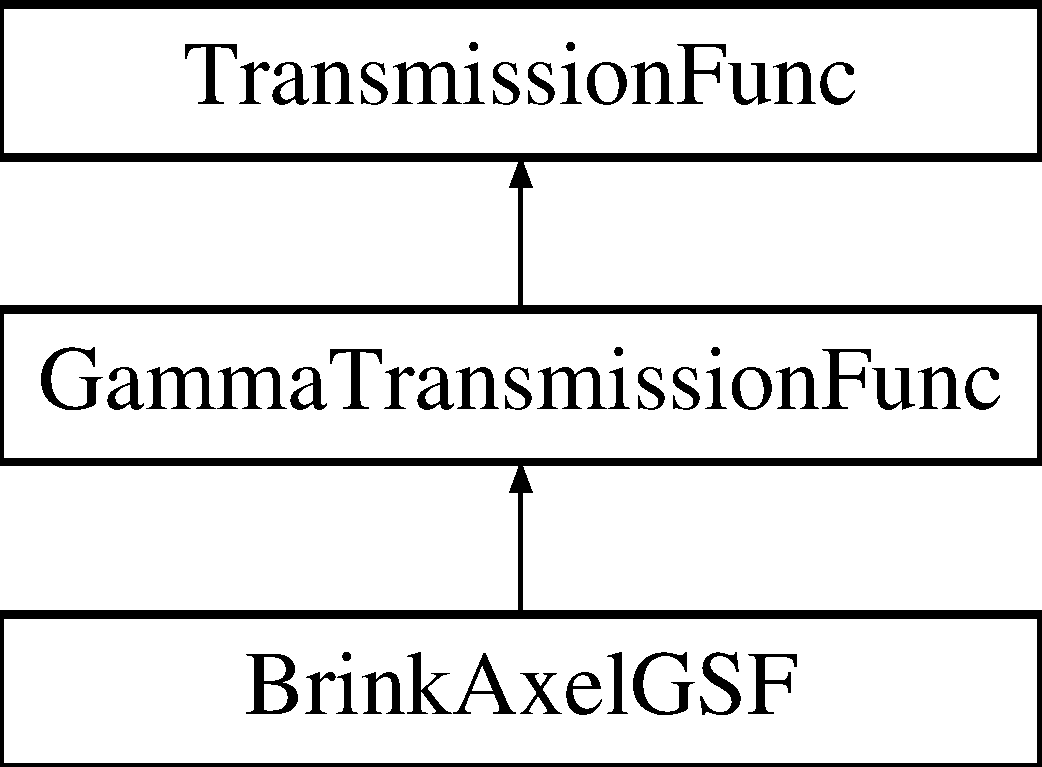
\includegraphics[height=3.000000cm]{d1/d51/classBrinkAxelGSF}
\end{center}
\end{figure}
\subsection*{Public Member Functions}
\begin{DoxyCompactItemize}
\item 
\hyperlink{classBrinkAxelGSF_aa90ed101a34e1d3013eff1434bdaab31}{Brink\-Axel\-G\-S\-F} (int, int, double, int, double, int, double, double, double, double, \hyperlink{classTransmissionFunc}{Transmission\-Func} $\ast$)
\item 
double \hyperlink{classBrinkAxelGSF_ac914ac4c34b969ea5b430e07199ed397}{Calc\-Strength\-Function} (double)
\end{DoxyCompactItemize}
\subsection*{Additional Inherited Members}


\subsection{Detailed Description}
Class for the Brink-\/\-Axel-\/\-G\-S\-F 

\subsection{Constructor \& Destructor Documentation}
\hypertarget{classBrinkAxelGSF_aa90ed101a34e1d3013eff1434bdaab31}{\index{Brink\-Axel\-G\-S\-F@{Brink\-Axel\-G\-S\-F}!Brink\-Axel\-G\-S\-F@{Brink\-Axel\-G\-S\-F}}
\index{Brink\-Axel\-G\-S\-F@{Brink\-Axel\-G\-S\-F}!BrinkAxelGSF@{Brink\-Axel\-G\-S\-F}}
\subsubsection[{Brink\-Axel\-G\-S\-F}]{\setlength{\rightskip}{0pt plus 5cm}Brink\-Axel\-G\-S\-F\-::\-Brink\-Axel\-G\-S\-F (
\begin{DoxyParamCaption}
\item[{int}]{z2, }
\item[{int}]{m2, }
\item[{double}]{j\-Initial, }
\item[{int}]{pi\-Initial, }
\item[{double}]{j\-Final, }
\item[{int}]{pi\-Final, }
\item[{double}]{max\-L, }
\item[{double}]{total\-Width\-For\-Correction, }
\item[{double}]{uncorr\-Total\-Width\-For\-Correction, }
\item[{double}]{uncorr\-Total\-Width\-Sqrd\-For\-Correction, }
\item[{{\bf Transmission\-Func} $\ast$}]{previous}
\end{DoxyParamCaption}
)}}\label{classBrinkAxelGSF_aa90ed101a34e1d3013eff1434bdaab31}
\hyperlink{BrinkAxelGSF_8h}{Brink\-Axel\-G\-S\-F.\-h} 

\subsection{Member Function Documentation}
\hypertarget{classBrinkAxelGSF_ac914ac4c34b969ea5b430e07199ed397}{\index{Brink\-Axel\-G\-S\-F@{Brink\-Axel\-G\-S\-F}!Calc\-Strength\-Function@{Calc\-Strength\-Function}}
\index{Calc\-Strength\-Function@{Calc\-Strength\-Function}!BrinkAxelGSF@{Brink\-Axel\-G\-S\-F}}
\subsubsection[{Calc\-Strength\-Function}]{\setlength{\rightskip}{0pt plus 5cm}double Brink\-Axel\-G\-S\-F\-::\-Calc\-Strength\-Function (
\begin{DoxyParamCaption}
\item[{double}]{energy}
\end{DoxyParamCaption}
)\hspace{0.3cm}{\ttfamily [virtual]}}}\label{classBrinkAxelGSF_ac914ac4c34b969ea5b430e07199ed397}


Implements \hyperlink{classGammaTransmissionFunc_a68156d72ed9620f66f96dc37bbf781aa}{Gamma\-Transmission\-Func}.



References G\-D\-R\-Parameters\-::\-E\-\_\-, Gamma\-Transmission\-Func\-::gdr\-Parameters\-\_\-, G\-D\-R\-Parameters\-::k\-Sigma\-Gamma\-\_\-, and Transmission\-Func\-::max\-L\-\_\-.



The documentation for this class was generated from the following files\-:\begin{DoxyCompactItemize}
\item 
/afs/crc.\-nd.\-edu/user/p/pscholz/\-Private/sapphire-\/devel/include/\hyperlink{BrinkAxelGSF_8h}{Brink\-Axel\-G\-S\-F.\-h}\item 
/afs/crc.\-nd.\-edu/user/p/pscholz/\-Private/sapphire-\/devel/src/\hyperlink{BrinkAxelGSF_8cpp}{Brink\-Axel\-G\-S\-F.\-cpp}\end{DoxyCompactItemize}

\hypertarget{classCDFEntry}{\section{C\-D\-F\-Entry Class Reference}
\label{classCDFEntry}\index{C\-D\-F\-Entry@{C\-D\-F\-Entry}}
}


{\ttfamily \#include $<$Decayer.\-h$>$}

\subsection*{Public Member Functions}
\begin{DoxyCompactItemize}
\item 
\hyperlink{classCDFEntry_a6b7a88d86e89bc25aaf860e490ca1607}{C\-D\-F\-Entry} (int pair\-Index, double energy, double value)
\end{DoxyCompactItemize}
\subsection*{Public Attributes}
\begin{DoxyCompactItemize}
\item 
int \hyperlink{classCDFEntry_abc2b0634d678993cbaf8b1451b38fc29}{pair\-Index\-\_\-}
\item 
double \hyperlink{classCDFEntry_a38595cb908b213effa5551bc11cf33ba}{energy\-\_\-}
\item 
double \hyperlink{classCDFEntry_a4f5ef593ff6dad671b8eb92ec4c3c7f7}{value\-\_\-}
\end{DoxyCompactItemize}


\subsection{Constructor \& Destructor Documentation}
\hypertarget{classCDFEntry_a6b7a88d86e89bc25aaf860e490ca1607}{\index{C\-D\-F\-Entry@{C\-D\-F\-Entry}!C\-D\-F\-Entry@{C\-D\-F\-Entry}}
\index{C\-D\-F\-Entry@{C\-D\-F\-Entry}!CDFEntry@{C\-D\-F\-Entry}}
\subsubsection[{C\-D\-F\-Entry}]{\setlength{\rightskip}{0pt plus 5cm}C\-D\-F\-Entry\-::\-C\-D\-F\-Entry (
\begin{DoxyParamCaption}
\item[{int}]{pair\-Index, }
\item[{double}]{energy, }
\item[{double}]{value}
\end{DoxyParamCaption}
)\hspace{0.3cm}{\ttfamily [inline]}}}\label{classCDFEntry_a6b7a88d86e89bc25aaf860e490ca1607}


\subsection{Member Data Documentation}
\hypertarget{classCDFEntry_a38595cb908b213effa5551bc11cf33ba}{\index{C\-D\-F\-Entry@{C\-D\-F\-Entry}!energy\-\_\-@{energy\-\_\-}}
\index{energy\-\_\-@{energy\-\_\-}!CDFEntry@{C\-D\-F\-Entry}}
\subsubsection[{energy\-\_\-}]{\setlength{\rightskip}{0pt plus 5cm}double C\-D\-F\-Entry\-::energy\-\_\-}}\label{classCDFEntry_a38595cb908b213effa5551bc11cf33ba}
\hypertarget{classCDFEntry_abc2b0634d678993cbaf8b1451b38fc29}{\index{C\-D\-F\-Entry@{C\-D\-F\-Entry}!pair\-Index\-\_\-@{pair\-Index\-\_\-}}
\index{pair\-Index\-\_\-@{pair\-Index\-\_\-}!CDFEntry@{C\-D\-F\-Entry}}
\subsubsection[{pair\-Index\-\_\-}]{\setlength{\rightskip}{0pt plus 5cm}int C\-D\-F\-Entry\-::pair\-Index\-\_\-}}\label{classCDFEntry_abc2b0634d678993cbaf8b1451b38fc29}
\hypertarget{classCDFEntry_a4f5ef593ff6dad671b8eb92ec4c3c7f7}{\index{C\-D\-F\-Entry@{C\-D\-F\-Entry}!value\-\_\-@{value\-\_\-}}
\index{value\-\_\-@{value\-\_\-}!CDFEntry@{C\-D\-F\-Entry}}
\subsubsection[{value\-\_\-}]{\setlength{\rightskip}{0pt plus 5cm}double C\-D\-F\-Entry\-::value\-\_\-}}\label{classCDFEntry_a4f5ef593ff6dad671b8eb92ec4c3c7f7}


The documentation for this class was generated from the following file\-:\begin{DoxyCompactItemize}
\item 
/afs/crc.\-nd.\-edu/user/p/pscholz/\-Private/sapphire-\/devel/include/\hyperlink{Decayer_8h}{Decayer.\-h}\end{DoxyCompactItemize}

\hypertarget{classCoulFunc}{\section{Coul\-Func Class Reference}
\label{classCoulFunc}\index{Coul\-Func@{Coul\-Func}}
}


{\ttfamily \#include $<$Coul\-Func.\-h$>$}

\subsection*{Public Member Functions}
\begin{DoxyCompactItemize}
\item 
\hyperlink{classCoulFunc_ae18ce8083cc140cf033fe242c5bc0279}{Coul\-Func} (int \hyperlink{classCoulFunc_a51a653c4ce27453d047b12cd9c259e60}{z1}, int \hyperlink{classCoulFunc_aa6bdb6af4163b9e2394123ad7daadedc}{z2}, double \hyperlink{classCoulFunc_a75d3ef5760151219ef16c916db221a83}{redmass}, bool use\-G\-S\-L\-Functions)
\item 
int \hyperlink{classCoulFunc_a51a653c4ce27453d047b12cd9c259e60}{z1} () const 
\item 
int \hyperlink{classCoulFunc_aa6bdb6af4163b9e2394123ad7daadedc}{z2} () const 
\item 
double \hyperlink{classCoulFunc_a75d3ef5760151219ef16c916db221a83}{redmass} () const 
\item 
int \hyperlink{classCoulFunc_af26580308c3aa3c6ed6d8010272e0cc3}{l\-Last} () const 
\item 
double \hyperlink{classCoulFunc_a294416dd0757533011ebfd56c9597739}{radius\-Last} () const 
\item 
double \hyperlink{classCoulFunc_ae6857b43f747e15e3948592cb68331f9}{energy\-Last} () const 
\item 
struct \hyperlink{structCoulWaves}{Coul\-Waves} \hyperlink{classCoulFunc_ac983b0b5fb84cc2065cca446ad392a7f}{coul\-Last} () const 
\item 
void \hyperlink{classCoulFunc_a42b754e3636f46c728c3fd1d07b38991}{set\-Last} (int, double, double, \hyperlink{structCoulWaves}{Coul\-Waves})
\item 
\hyperlink{structCoulWaves}{Coul\-Waves} \hyperlink{classCoulFunc_ab8e9ec2de76a9d91f127808668bc09c7}{operator()} (int, double, double)
\item 
double \hyperlink{classCoulFunc_ac8b8f683db1e485c996ae74273dfa79e}{Penetrability} (int, double, double)
\item 
double \hyperlink{classCoulFunc_aecd3469fbf1a12ac6269e287c39b9ed3}{P\-E\-Shift} (int, double, double)
\item 
double \hyperlink{classCoulFunc_a25e6977287af90803d47eb70a2433ce0}{P\-E\-Shift\-\_\-d\-E} (int, double, double)
\end{DoxyCompactItemize}
\subsection*{Static Public Member Functions}
\begin{DoxyCompactItemize}
\item 
static void \hyperlink{classCoulFunc_abbea8a2c1df9d4dda1635b30c3e195d2}{G\-S\-L\-Error\-Handler} (const char $\ast$, const char $\ast$, int, int)
\end{DoxyCompactItemize}


\subsection{Constructor \& Destructor Documentation}
\hypertarget{classCoulFunc_ae18ce8083cc140cf033fe242c5bc0279}{\index{Coul\-Func@{Coul\-Func}!Coul\-Func@{Coul\-Func}}
\index{Coul\-Func@{Coul\-Func}!CoulFunc@{Coul\-Func}}
\subsubsection[{Coul\-Func}]{\setlength{\rightskip}{0pt plus 5cm}Coul\-Func\-::\-Coul\-Func (
\begin{DoxyParamCaption}
\item[{int}]{z1, }
\item[{int}]{z2, }
\item[{double}]{redmass, }
\item[{bool}]{use\-G\-S\-L\-Functions}
\end{DoxyParamCaption}
)}}\label{classCoulFunc_ae18ce8083cc140cf033fe242c5bc0279}


References Coul\-Waves\-::d\-F, Coul\-Waves\-::d\-G, Coul\-Waves\-::\-F, and Coul\-Waves\-::\-G.



\subsection{Member Function Documentation}
\hypertarget{classCoulFunc_ac983b0b5fb84cc2065cca446ad392a7f}{\index{Coul\-Func@{Coul\-Func}!coul\-Last@{coul\-Last}}
\index{coul\-Last@{coul\-Last}!CoulFunc@{Coul\-Func}}
\subsubsection[{coul\-Last}]{\setlength{\rightskip}{0pt plus 5cm}struct {\bf Coul\-Waves} Coul\-Func\-::coul\-Last (
\begin{DoxyParamCaption}
{}
\end{DoxyParamCaption}
) const}}\label{classCoulFunc_ac983b0b5fb84cc2065cca446ad392a7f}
Returns the last Coulomb functions which were calculated. 

Referenced by operator()().

\hypertarget{classCoulFunc_ae6857b43f747e15e3948592cb68331f9}{\index{Coul\-Func@{Coul\-Func}!energy\-Last@{energy\-Last}}
\index{energy\-Last@{energy\-Last}!CoulFunc@{Coul\-Func}}
\subsubsection[{energy\-Last}]{\setlength{\rightskip}{0pt plus 5cm}double Coul\-Func\-::energy\-Last (
\begin{DoxyParamCaption}
{}
\end{DoxyParamCaption}
) const}}\label{classCoulFunc_ae6857b43f747e15e3948592cb68331f9}
Returns the last energy value at which the Coulomb functions were calculated. 

Referenced by operator()().

\hypertarget{classCoulFunc_abbea8a2c1df9d4dda1635b30c3e195d2}{\index{Coul\-Func@{Coul\-Func}!G\-S\-L\-Error\-Handler@{G\-S\-L\-Error\-Handler}}
\index{G\-S\-L\-Error\-Handler@{G\-S\-L\-Error\-Handler}!CoulFunc@{Coul\-Func}}
\subsubsection[{G\-S\-L\-Error\-Handler}]{\setlength{\rightskip}{0pt plus 5cm}void Coul\-Func\-::\-G\-S\-L\-Error\-Handler (
\begin{DoxyParamCaption}
\item[{const char $\ast$}]{reason, }
\item[{const char $\ast$}]{file, }
\item[{int}]{line, }
\item[{int}]{error\-Code}
\end{DoxyParamCaption}
)\hspace{0.3cm}{\ttfamily [static]}}}\label{classCoulFunc_abbea8a2c1df9d4dda1635b30c3e195d2}


Referenced by Initialize().

\hypertarget{classCoulFunc_af26580308c3aa3c6ed6d8010272e0cc3}{\index{Coul\-Func@{Coul\-Func}!l\-Last@{l\-Last}}
\index{l\-Last@{l\-Last}!CoulFunc@{Coul\-Func}}
\subsubsection[{l\-Last}]{\setlength{\rightskip}{0pt plus 5cm}int Coul\-Func\-::l\-Last (
\begin{DoxyParamCaption}
{}
\end{DoxyParamCaption}
) const}}\label{classCoulFunc_af26580308c3aa3c6ed6d8010272e0cc3}
Returns the last orbital angular momentum value at which the Coulomb functions were calculated. 

Referenced by operator()(), and set\-Last().

\hypertarget{classCoulFunc_ab8e9ec2de76a9d91f127808668bc09c7}{\index{Coul\-Func@{Coul\-Func}!operator()@{operator()}}
\index{operator()@{operator()}!CoulFunc@{Coul\-Func}}
\subsubsection[{operator()}]{\setlength{\rightskip}{0pt plus 5cm}{\bf Coul\-Waves} Coul\-Func\-::operator() (
\begin{DoxyParamCaption}
\item[{int}]{l, }
\item[{double}]{radius, }
\item[{double}]{energy}
\end{DoxyParamCaption}
)}}\label{classCoulFunc_ab8e9ec2de76a9d91f127808668bc09c7}
The parenthesis operator is defined to make the class instance callable as a function. The orbital angular momentum, radius, and energy in the center of mass system are the dependent variables. The function returns the Coulomb waves. 

References coul\-Last(), Coul\-Waves\-::d\-F, Coul\-Waves\-::d\-G, energy\-Last(), Coul\-Waves\-::\-F, Coulomb\-\_\-wave\-\_\-functions\-::\-F\-\_\-d\-F(), fstruc, Coul\-Waves\-::\-G, Coulomb\-\_\-wave\-\_\-functions\-::\-G\-\_\-d\-G(), hbarc, l\-Last(), radius\-Last(), redmass(), uconv, z1(), and z2().



Referenced by Penetrability(), and P\-E\-Shift().

\hypertarget{classCoulFunc_ac8b8f683db1e485c996ae74273dfa79e}{\index{Coul\-Func@{Coul\-Func}!Penetrability@{Penetrability}}
\index{Penetrability@{Penetrability}!CoulFunc@{Coul\-Func}}
\subsubsection[{Penetrability}]{\setlength{\rightskip}{0pt plus 5cm}double Coul\-Func\-::\-Penetrability (
\begin{DoxyParamCaption}
\item[{int}]{l, }
\item[{double}]{radius, }
\item[{double}]{energy}
\end{DoxyParamCaption}
)}}\label{classCoulFunc_ac8b8f683db1e485c996ae74273dfa79e}
Returns the penetrability as a function of orbital angular momentum, radius, and energy in the center of mass system. 

References Coul\-Waves\-::\-F, Coul\-Waves\-::\-G, hbarc, operator()(), redmass(), and uconv.



Referenced by Equiv\-Square\-Well\-::\-Calc\-Transmission().

\hypertarget{classCoulFunc_aecd3469fbf1a12ac6269e287c39b9ed3}{\index{Coul\-Func@{Coul\-Func}!P\-E\-Shift@{P\-E\-Shift}}
\index{P\-E\-Shift@{P\-E\-Shift}!CoulFunc@{Coul\-Func}}
\subsubsection[{P\-E\-Shift}]{\setlength{\rightskip}{0pt plus 5cm}double Coul\-Func\-::\-P\-E\-Shift (
\begin{DoxyParamCaption}
\item[{int}]{l, }
\item[{double}]{radius, }
\item[{double}]{energy}
\end{DoxyParamCaption}
)}}\label{classCoulFunc_aecd3469fbf1a12ac6269e287c39b9ed3}
Returns the positive energy shift function a function of orbital angular momentum, radius, and energy in the center of mass system. 

References Coul\-Waves\-::d\-F, Coul\-Waves\-::d\-G, Coul\-Waves\-::\-F, Coul\-Waves\-::\-G, hbarc, operator()(), redmass(), and uconv.

\hypertarget{classCoulFunc_a25e6977287af90803d47eb70a2433ce0}{\index{Coul\-Func@{Coul\-Func}!P\-E\-Shift\-\_\-d\-E@{P\-E\-Shift\-\_\-d\-E}}
\index{P\-E\-Shift\-\_\-d\-E@{P\-E\-Shift\-\_\-d\-E}!CoulFunc@{Coul\-Func}}
\subsubsection[{P\-E\-Shift\-\_\-d\-E}]{\setlength{\rightskip}{0pt plus 5cm}double Coul\-Func\-::\-P\-E\-Shift\-\_\-d\-E (
\begin{DoxyParamCaption}
\item[{int}]{l, }
\item[{double}]{radius, }
\item[{double}]{energy}
\end{DoxyParamCaption}
)}}\label{classCoulFunc_a25e6977287af90803d47eb70a2433ce0}
Returns the energy derivative of the shift function a function of orbital angular momentum, radius, and energy in the center of mass system. 

References Coul\-Waves\-::\-F.

\hypertarget{classCoulFunc_a294416dd0757533011ebfd56c9597739}{\index{Coul\-Func@{Coul\-Func}!radius\-Last@{radius\-Last}}
\index{radius\-Last@{radius\-Last}!CoulFunc@{Coul\-Func}}
\subsubsection[{radius\-Last}]{\setlength{\rightskip}{0pt plus 5cm}double Coul\-Func\-::radius\-Last (
\begin{DoxyParamCaption}
{}
\end{DoxyParamCaption}
) const}}\label{classCoulFunc_a294416dd0757533011ebfd56c9597739}
Returns the last radius value at which the Coulomb functions were calculated. 

Referenced by operator()().

\hypertarget{classCoulFunc_a75d3ef5760151219ef16c916db221a83}{\index{Coul\-Func@{Coul\-Func}!redmass@{redmass}}
\index{redmass@{redmass}!CoulFunc@{Coul\-Func}}
\subsubsection[{redmass}]{\setlength{\rightskip}{0pt plus 5cm}double Coul\-Func\-::redmass (
\begin{DoxyParamCaption}
{}
\end{DoxyParamCaption}
) const}}\label{classCoulFunc_a75d3ef5760151219ef16c916db221a83}
Returns the reduced mass of the particle pair. 

Referenced by operator()(), Penetrability(), and P\-E\-Shift().

\hypertarget{classCoulFunc_a42b754e3636f46c728c3fd1d07b38991}{\index{Coul\-Func@{Coul\-Func}!set\-Last@{set\-Last}}
\index{set\-Last@{set\-Last}!CoulFunc@{Coul\-Func}}
\subsubsection[{set\-Last}]{\setlength{\rightskip}{0pt plus 5cm}void Coul\-Func\-::set\-Last (
\begin{DoxyParamCaption}
\item[{int}]{l\-Last, }
\item[{double}]{r\-Last, }
\item[{double}]{e\-Last, }
\item[{{\bf Coul\-Waves}}]{coul\-Last}
\end{DoxyParamCaption}
)}}\label{classCoulFunc_a42b754e3636f46c728c3fd1d07b38991}
Sets the last calculated Coulomb waves and the values for which they were calculated. 

References Coul\-Waves\-::d\-F, Coul\-Waves\-::d\-G, Coul\-Waves\-::\-F, Coul\-Waves\-::\-G, and l\-Last().

\hypertarget{classCoulFunc_a51a653c4ce27453d047b12cd9c259e60}{\index{Coul\-Func@{Coul\-Func}!z1@{z1}}
\index{z1@{z1}!CoulFunc@{Coul\-Func}}
\subsubsection[{z1}]{\setlength{\rightskip}{0pt plus 5cm}int Coul\-Func\-::z1 (
\begin{DoxyParamCaption}
{}
\end{DoxyParamCaption}
) const}}\label{classCoulFunc_a51a653c4ce27453d047b12cd9c259e60}
Returns the atomic number of the first particle in the pair. 

Referenced by operator()().

\hypertarget{classCoulFunc_aa6bdb6af4163b9e2394123ad7daadedc}{\index{Coul\-Func@{Coul\-Func}!z2@{z2}}
\index{z2@{z2}!CoulFunc@{Coul\-Func}}
\subsubsection[{z2}]{\setlength{\rightskip}{0pt plus 5cm}int Coul\-Func\-::z2 (
\begin{DoxyParamCaption}
{}
\end{DoxyParamCaption}
) const}}\label{classCoulFunc_aa6bdb6af4163b9e2394123ad7daadedc}
Returns the atomic number of the second particle in the pair. 

Referenced by operator()().



The documentation for this class was generated from the following files\-:\begin{DoxyCompactItemize}
\item 
include/\hyperlink{CoulFunc_8h}{Coul\-Func.\-h}\item 
src/\hyperlink{CoulFunc_8cpp}{Coul\-Func.\-cpp}\end{DoxyCompactItemize}

\hypertarget{classCoulomb__wave__functions}{\section{Coulomb\-\_\-wave\-\_\-functions Class Reference}
\label{classCoulomb__wave__functions}\index{Coulomb\-\_\-wave\-\_\-functions@{Coulomb\-\_\-wave\-\_\-functions}}
}


{\ttfamily \#include $<$cwfcomp.\-H$>$}

\subsection*{Public Member Functions}
\begin{DoxyCompactItemize}
\item 
\hyperlink{classCoulomb__wave__functions_ac1d33cc04d9c2629d0339772277a9cc8}{Coulomb\-\_\-wave\-\_\-functions} (const bool is\-\_\-it\-\_\-normalized\-\_\-c, const \hyperlink{Constants_8h_a1c1b16cc02d518bbe753449171ab7033}{std\-::complex}$<$ double $>$ \&l\-\_\-c, const \hyperlink{Constants_8h_a1c1b16cc02d518bbe753449171ab7033}{std\-::complex}$<$ double $>$ \&eta\-\_\-c)
\item 
\hyperlink{classCoulomb__wave__functions_a22b1bddeeeeaeb8ef0ea7fab9084fbf3}{$\sim$\-Coulomb\-\_\-wave\-\_\-functions} (void)
\item 
void \hyperlink{classCoulomb__wave__functions_a6b3367113a7be7ef3b23b15a24dccceb}{F\-\_\-d\-F\-\_\-init} (const \hyperlink{Constants_8h_a1c1b16cc02d518bbe753449171ab7033}{std\-::complex}$<$ double $>$ \&z, const \hyperlink{Constants_8h_a1c1b16cc02d518bbe753449171ab7033}{std\-::complex}$<$ double $>$ \&F, const \hyperlink{Constants_8h_a1c1b16cc02d518bbe753449171ab7033}{std\-::complex}$<$ double $>$ \&d\-F)
\item 
void \hyperlink{classCoulomb__wave__functions_aa50c907890ba95453087824914c3a90b}{F\-\_\-d\-F} (const \hyperlink{Constants_8h_a1c1b16cc02d518bbe753449171ab7033}{std\-::complex}$<$ double $>$ \&z, \hyperlink{Constants_8h_a1c1b16cc02d518bbe753449171ab7033}{std\-::complex}$<$ double $>$ \&F, \hyperlink{Constants_8h_a1c1b16cc02d518bbe753449171ab7033}{std\-::complex}$<$ double $>$ \&d\-F)
\item 
void \hyperlink{classCoulomb__wave__functions_a290186f37ddca40667af2a0acb031fcb}{G\-\_\-d\-G} (const \hyperlink{Constants_8h_a1c1b16cc02d518bbe753449171ab7033}{std\-::complex}$<$ double $>$ \&z, \hyperlink{Constants_8h_a1c1b16cc02d518bbe753449171ab7033}{std\-::complex}$<$ double $>$ \&G, \hyperlink{Constants_8h_a1c1b16cc02d518bbe753449171ab7033}{std\-::complex}$<$ double $>$ \&d\-G)
\item 
void \hyperlink{classCoulomb__wave__functions_aed77d82a52638ff69f9526ad7504795f}{H\-\_\-d\-H} (const int omega, const \hyperlink{Constants_8h_a1c1b16cc02d518bbe753449171ab7033}{std\-::complex}$<$ double $>$ \&z, \hyperlink{Constants_8h_a1c1b16cc02d518bbe753449171ab7033}{std\-::complex}$<$ double $>$ \&H, \hyperlink{Constants_8h_a1c1b16cc02d518bbe753449171ab7033}{std\-::complex}$<$ double $>$ \&d\-H)
\item 
void \hyperlink{classCoulomb__wave__functions_a4820d8d44ee5c5e9193c8950e98935c2}{H\-\_\-d\-H\-\_\-scaled} (const int omega, const \hyperlink{Constants_8h_a1c1b16cc02d518bbe753449171ab7033}{std\-::complex}$<$ double $>$ \&z, \hyperlink{Constants_8h_a1c1b16cc02d518bbe753449171ab7033}{std\-::complex}$<$ double $>$ \&H, \hyperlink{Constants_8h_a1c1b16cc02d518bbe753449171ab7033}{std\-::complex}$<$ double $>$ \&d\-H)
\end{DoxyCompactItemize}
\subsection*{Public Attributes}
\begin{DoxyCompactItemize}
\item 
const \hyperlink{Constants_8h_a1c1b16cc02d518bbe753449171ab7033}{std\-::complex}$<$ double $>$ \hyperlink{classCoulomb__wave__functions_a184f08ca7adeb5d334b72dc354777a64}{l}
\item 
const \hyperlink{Constants_8h_a1c1b16cc02d518bbe753449171ab7033}{std\-::complex}$<$ double $>$ \hyperlink{classCoulomb__wave__functions_a944d6723016c4c50ad7a9b55d62a0131}{eta}
\item 
const bool \hyperlink{classCoulomb__wave__functions_a11b791087220f0194b2750d36946392e}{is\-\_\-it\-\_\-normalized}
\end{DoxyCompactItemize}


\subsection{Constructor \& Destructor Documentation}
\hypertarget{classCoulomb__wave__functions_ac1d33cc04d9c2629d0339772277a9cc8}{\index{Coulomb\-\_\-wave\-\_\-functions@{Coulomb\-\_\-wave\-\_\-functions}!Coulomb\-\_\-wave\-\_\-functions@{Coulomb\-\_\-wave\-\_\-functions}}
\index{Coulomb\-\_\-wave\-\_\-functions@{Coulomb\-\_\-wave\-\_\-functions}!Coulomb_wave_functions@{Coulomb\-\_\-wave\-\_\-functions}}
\subsubsection[{Coulomb\-\_\-wave\-\_\-functions}]{\setlength{\rightskip}{0pt plus 5cm}Coulomb\-\_\-wave\-\_\-functions\-::\-Coulomb\-\_\-wave\-\_\-functions (
\begin{DoxyParamCaption}
\item[{const bool}]{is\-\_\-it\-\_\-normalized\-\_\-c, }
\item[{const {\bf std\-::complex}$<$ double $>$ \&}]{l\-\_\-c, }
\item[{const {\bf std\-::complex}$<$ double $>$ \&}]{eta\-\_\-c}
\end{DoxyParamCaption}
)\hspace{0.3cm}{\ttfamily [inline]}}}\label{classCoulomb__wave__functions_ac1d33cc04d9c2629d0339772277a9cc8}


References eta, and is\-\_\-it\-\_\-normalized.

\hypertarget{classCoulomb__wave__functions_a22b1bddeeeeaeb8ef0ea7fab9084fbf3}{\index{Coulomb\-\_\-wave\-\_\-functions@{Coulomb\-\_\-wave\-\_\-functions}!$\sim$\-Coulomb\-\_\-wave\-\_\-functions@{$\sim$\-Coulomb\-\_\-wave\-\_\-functions}}
\index{$\sim$\-Coulomb\-\_\-wave\-\_\-functions@{$\sim$\-Coulomb\-\_\-wave\-\_\-functions}!Coulomb_wave_functions@{Coulomb\-\_\-wave\-\_\-functions}}
\subsubsection[{$\sim$\-Coulomb\-\_\-wave\-\_\-functions}]{\setlength{\rightskip}{0pt plus 5cm}Coulomb\-\_\-wave\-\_\-functions\-::$\sim$\-Coulomb\-\_\-wave\-\_\-functions (
\begin{DoxyParamCaption}
\item[{void}]{}
\end{DoxyParamCaption}
)\hspace{0.3cm}{\ttfamily [inline]}}}\label{classCoulomb__wave__functions_a22b1bddeeeeaeb8ef0ea7fab9084fbf3}


\subsection{Member Function Documentation}
\hypertarget{classCoulomb__wave__functions_aa50c907890ba95453087824914c3a90b}{\index{Coulomb\-\_\-wave\-\_\-functions@{Coulomb\-\_\-wave\-\_\-functions}!F\-\_\-d\-F@{F\-\_\-d\-F}}
\index{F\-\_\-d\-F@{F\-\_\-d\-F}!Coulomb_wave_functions@{Coulomb\-\_\-wave\-\_\-functions}}
\subsubsection[{F\-\_\-d\-F}]{\setlength{\rightskip}{0pt plus 5cm}void Coulomb\-\_\-wave\-\_\-functions\-::\-F\-\_\-d\-F (
\begin{DoxyParamCaption}
\item[{const {\bf std\-::complex}$<$ double $>$ \&}]{z, }
\item[{{\bf std\-::complex}$<$ double $>$ \&}]{F, }
\item[{{\bf std\-::complex}$<$ double $>$ \&}]{d\-F}
\end{DoxyParamCaption}
)}}\label{classCoulomb__wave__functions_aa50c907890ba95453087824914c3a90b}


References is\-\_\-it\-\_\-normalized, isfinite(), S\-I\-G\-N, and sqrt\-\_\-precision.



Referenced by G\-\_\-d\-G(), H\-\_\-d\-H(), H\-\_\-d\-H\-\_\-scaled(), and Coul\-Func\-::operator()().

\hypertarget{classCoulomb__wave__functions_a6b3367113a7be7ef3b23b15a24dccceb}{\index{Coulomb\-\_\-wave\-\_\-functions@{Coulomb\-\_\-wave\-\_\-functions}!F\-\_\-d\-F\-\_\-init@{F\-\_\-d\-F\-\_\-init}}
\index{F\-\_\-d\-F\-\_\-init@{F\-\_\-d\-F\-\_\-init}!Coulomb_wave_functions@{Coulomb\-\_\-wave\-\_\-functions}}
\subsubsection[{F\-\_\-d\-F\-\_\-init}]{\setlength{\rightskip}{0pt plus 5cm}void Coulomb\-\_\-wave\-\_\-functions\-::\-F\-\_\-d\-F\-\_\-init (
\begin{DoxyParamCaption}
\item[{const {\bf std\-::complex}$<$ double $>$ \&}]{z, }
\item[{const {\bf std\-::complex}$<$ double $>$ \&}]{F, }
\item[{const {\bf std\-::complex}$<$ double $>$ \&}]{d\-F}
\end{DoxyParamCaption}
)}}\label{classCoulomb__wave__functions_a6b3367113a7be7ef3b23b15a24dccceb}
\hypertarget{classCoulomb__wave__functions_a290186f37ddca40667af2a0acb031fcb}{\index{Coulomb\-\_\-wave\-\_\-functions@{Coulomb\-\_\-wave\-\_\-functions}!G\-\_\-d\-G@{G\-\_\-d\-G}}
\index{G\-\_\-d\-G@{G\-\_\-d\-G}!Coulomb_wave_functions@{Coulomb\-\_\-wave\-\_\-functions}}
\subsubsection[{G\-\_\-d\-G}]{\setlength{\rightskip}{0pt plus 5cm}void Coulomb\-\_\-wave\-\_\-functions\-::\-G\-\_\-d\-G (
\begin{DoxyParamCaption}
\item[{const {\bf std\-::complex}$<$ double $>$ \&}]{z, }
\item[{{\bf std\-::complex}$<$ double $>$ \&}]{G, }
\item[{{\bf std\-::complex}$<$ double $>$ \&}]{d\-G}
\end{DoxyParamCaption}
)}}\label{classCoulomb__wave__functions_a290186f37ddca40667af2a0acb031fcb}


References F\-\_\-d\-F(), H\-\_\-d\-H(), is\-\_\-it\-\_\-normalized, isfinite(), and sqrt\-\_\-precision.



Referenced by Coul\-Func\-::operator()().

\hypertarget{classCoulomb__wave__functions_aed77d82a52638ff69f9526ad7504795f}{\index{Coulomb\-\_\-wave\-\_\-functions@{Coulomb\-\_\-wave\-\_\-functions}!H\-\_\-d\-H@{H\-\_\-d\-H}}
\index{H\-\_\-d\-H@{H\-\_\-d\-H}!Coulomb_wave_functions@{Coulomb\-\_\-wave\-\_\-functions}}
\subsubsection[{H\-\_\-d\-H}]{\setlength{\rightskip}{0pt plus 5cm}void Coulomb\-\_\-wave\-\_\-functions\-::\-H\-\_\-d\-H (
\begin{DoxyParamCaption}
\item[{const int}]{omega, }
\item[{const {\bf std\-::complex}$<$ double $>$ \&}]{z, }
\item[{{\bf std\-::complex}$<$ double $>$ \&}]{H, }
\item[{{\bf std\-::complex}$<$ double $>$ \&}]{d\-H}
\end{DoxyParamCaption}
)}}\label{classCoulomb__wave__functions_aed77d82a52638ff69f9526ad7504795f}


References F\-\_\-d\-F(), is\-\_\-it\-\_\-normalized, isfinite(), and sqrt\-\_\-precision.



Referenced by G\-\_\-d\-G().

\hypertarget{classCoulomb__wave__functions_a4820d8d44ee5c5e9193c8950e98935c2}{\index{Coulomb\-\_\-wave\-\_\-functions@{Coulomb\-\_\-wave\-\_\-functions}!H\-\_\-d\-H\-\_\-scaled@{H\-\_\-d\-H\-\_\-scaled}}
\index{H\-\_\-d\-H\-\_\-scaled@{H\-\_\-d\-H\-\_\-scaled}!Coulomb_wave_functions@{Coulomb\-\_\-wave\-\_\-functions}}
\subsubsection[{H\-\_\-d\-H\-\_\-scaled}]{\setlength{\rightskip}{0pt plus 5cm}void Coulomb\-\_\-wave\-\_\-functions\-::\-H\-\_\-d\-H\-\_\-scaled (
\begin{DoxyParamCaption}
\item[{const int}]{omega, }
\item[{const {\bf std\-::complex}$<$ double $>$ \&}]{z, }
\item[{{\bf std\-::complex}$<$ double $>$ \&}]{H, }
\item[{{\bf std\-::complex}$<$ double $>$ \&}]{d\-H}
\end{DoxyParamCaption}
)}}\label{classCoulomb__wave__functions_a4820d8d44ee5c5e9193c8950e98935c2}


References F\-\_\-d\-F(), is\-\_\-it\-\_\-normalized, isfinite(), and sqrt\-\_\-precision.



\subsection{Member Data Documentation}
\hypertarget{classCoulomb__wave__functions_a944d6723016c4c50ad7a9b55d62a0131}{\index{Coulomb\-\_\-wave\-\_\-functions@{Coulomb\-\_\-wave\-\_\-functions}!eta@{eta}}
\index{eta@{eta}!Coulomb_wave_functions@{Coulomb\-\_\-wave\-\_\-functions}}
\subsubsection[{eta}]{\setlength{\rightskip}{0pt plus 5cm}const {\bf std\-::complex}$<$double$>$ Coulomb\-\_\-wave\-\_\-functions\-::eta}}\label{classCoulomb__wave__functions_a944d6723016c4c50ad7a9b55d62a0131}


Referenced by Coulomb\-\_\-wave\-\_\-functions().

\hypertarget{classCoulomb__wave__functions_a11b791087220f0194b2750d36946392e}{\index{Coulomb\-\_\-wave\-\_\-functions@{Coulomb\-\_\-wave\-\_\-functions}!is\-\_\-it\-\_\-normalized@{is\-\_\-it\-\_\-normalized}}
\index{is\-\_\-it\-\_\-normalized@{is\-\_\-it\-\_\-normalized}!Coulomb_wave_functions@{Coulomb\-\_\-wave\-\_\-functions}}
\subsubsection[{is\-\_\-it\-\_\-normalized}]{\setlength{\rightskip}{0pt plus 5cm}const bool Coulomb\-\_\-wave\-\_\-functions\-::is\-\_\-it\-\_\-normalized}}\label{classCoulomb__wave__functions_a11b791087220f0194b2750d36946392e}


Referenced by Coulomb\-\_\-wave\-\_\-functions(), F\-\_\-d\-F(), G\-\_\-d\-G(), H\-\_\-d\-H(), and H\-\_\-d\-H\-\_\-scaled().

\hypertarget{classCoulomb__wave__functions_a184f08ca7adeb5d334b72dc354777a64}{\index{Coulomb\-\_\-wave\-\_\-functions@{Coulomb\-\_\-wave\-\_\-functions}!l@{l}}
\index{l@{l}!Coulomb_wave_functions@{Coulomb\-\_\-wave\-\_\-functions}}
\subsubsection[{l}]{\setlength{\rightskip}{0pt plus 5cm}const {\bf std\-::complex}$<$double$>$ Coulomb\-\_\-wave\-\_\-functions\-::l}}\label{classCoulomb__wave__functions_a184f08ca7adeb5d334b72dc354777a64}


The documentation for this class was generated from the following files\-:\begin{DoxyCompactItemize}
\item 
coul/include/\hyperlink{cwfcomp_8H}{cwfcomp.\-H}\item 
coul/src/\hyperlink{cwfcomp_8cpp}{cwfcomp.\-cpp}\end{DoxyCompactItemize}

\hypertarget{structCoulWaves}{\section{Coul\-Waves Struct Reference}
\label{structCoulWaves}\index{Coul\-Waves@{Coul\-Waves}}
}


{\ttfamily \#include $<$Coul\-Func.\-h$>$}

\subsection*{Public Attributes}
\begin{DoxyCompactItemize}
\item 
double \hyperlink{structCoulWaves_ad04a2d9552d7cfc775f35cd179000553}{F}
\item 
double \hyperlink{structCoulWaves_ac85f757250d93923d47519f4b8f13117}{d\-F}
\item 
double \hyperlink{structCoulWaves_a6ed564ba02c1d0b75b2453f8129eae48}{G}
\item 
double \hyperlink{structCoulWaves_a8eea43731321d6e28f5ecba6d73f0174}{d\-G}
\end{DoxyCompactItemize}


\subsection{Member Data Documentation}
\hypertarget{structCoulWaves_ac85f757250d93923d47519f4b8f13117}{\index{Coul\-Waves@{Coul\-Waves}!d\-F@{d\-F}}
\index{d\-F@{d\-F}!CoulWaves@{Coul\-Waves}}
\subsubsection[{d\-F}]{\setlength{\rightskip}{0pt plus 5cm}double Coul\-Waves\-::d\-F}}\label{structCoulWaves_ac85f757250d93923d47519f4b8f13117}


Referenced by Potential\-::\-Calc\-Transmission(), Coul\-Func\-::\-Coul\-Func(), Coul\-Func\-::operator()(), Coul\-Func\-::\-P\-E\-Shift(), and Coul\-Func\-::set\-Last().

\hypertarget{structCoulWaves_a8eea43731321d6e28f5ecba6d73f0174}{\index{Coul\-Waves@{Coul\-Waves}!d\-G@{d\-G}}
\index{d\-G@{d\-G}!CoulWaves@{Coul\-Waves}}
\subsubsection[{d\-G}]{\setlength{\rightskip}{0pt plus 5cm}double Coul\-Waves\-::d\-G}}\label{structCoulWaves_a8eea43731321d6e28f5ecba6d73f0174}


Referenced by Potential\-::\-Calc\-Transmission(), Coul\-Func\-::\-Coul\-Func(), Coul\-Func\-::operator()(), Coul\-Func\-::\-P\-E\-Shift(), and Coul\-Func\-::set\-Last().

\hypertarget{structCoulWaves_ad04a2d9552d7cfc775f35cd179000553}{\index{Coul\-Waves@{Coul\-Waves}!F@{F}}
\index{F@{F}!CoulWaves@{Coul\-Waves}}
\subsubsection[{F}]{\setlength{\rightskip}{0pt plus 5cm}double Coul\-Waves\-::\-F}}\label{structCoulWaves_ad04a2d9552d7cfc775f35cd179000553}


Referenced by Potential\-::\-Calc\-Transmission(), Coul\-Func\-::\-Coul\-Func(), Coul\-Func\-::operator()(), Coul\-Func\-::\-Penetrability(), Coul\-Func\-::\-P\-E\-Shift(), Coul\-Func\-::\-P\-E\-Shift\-\_\-d\-E(), and Coul\-Func\-::set\-Last().

\hypertarget{structCoulWaves_a6ed564ba02c1d0b75b2453f8129eae48}{\index{Coul\-Waves@{Coul\-Waves}!G@{G}}
\index{G@{G}!CoulWaves@{Coul\-Waves}}
\subsubsection[{G}]{\setlength{\rightskip}{0pt plus 5cm}double Coul\-Waves\-::\-G}}\label{structCoulWaves_a6ed564ba02c1d0b75b2453f8129eae48}


Referenced by Potential\-::\-Calc\-Transmission(), Coul\-Func\-::\-Coul\-Func(), Coul\-Func\-::operator()(), Coul\-Func\-::\-Penetrability(), Coul\-Func\-::\-P\-E\-Shift(), and Coul\-Func\-::set\-Last().



The documentation for this struct was generated from the following file\-:\begin{DoxyCompactItemize}
\item 
include/\hyperlink{CoulFunc_8h}{Coul\-Func.\-h}\end{DoxyCompactItemize}

\hypertarget{classCrossSection}{\section{Cross\-Section Class Reference}
\label{classCrossSection}\index{Cross\-Section@{Cross\-Section}}
}


{\ttfamily \#include $<$Cross\-Section.\-h$>$}

\subsection*{Public Member Functions}
\begin{DoxyCompactItemize}
\item 
\hyperlink{classCrossSection_a1b6153b04abfedf530ec16b61a037675}{Cross\-Section} (int, int, int, std\-::string, bool, int entrance\-State=0, std\-::vector$<$ int $>$ exit\-States=std\-::vector$<$ int $>$(4,-\/1))
\item 
bool \hyperlink{classCrossSection_af9d7861a745a315774a300ad76b462e9}{Is\-Valid} () const 
\item 
void \hyperlink{classCrossSection_a7a9c110cc504c1e4a1dcfde56c1a9fc3}{Calculate} ()
\item 
void \hyperlink{classCrossSection_a63f9594f0d5bd585a782efd1194684e7}{Print\-Cross\-Sections} ()
\item 
void \hyperlink{classCrossSection_a92572bb7b0d827adf25f2d85406c3975}{Print\-Transmission\-Terms} ()
\item 
std\-::pair$<$ double, double $>$ \hyperlink{classCrossSection_a8f565b6ac64e6926e048cb616057c7fe}{Calc\-Average\-S\-Wave\-Res\-Width} ()
\item 
std\-::pair$<$ double, double $>$ \hyperlink{classCrossSection_ab8fcc59ed5ef9eaa09140b59b31f16f3}{Calc\-Average\-P\-Wave\-Res\-Width} ()
\item 
std\-::pair$<$ double, double $>$ \hyperlink{classCrossSection_ae910a6a04f52aa52065faf03f52a2af1}{Calc\-Average\-D\-Wave\-Res\-Width} ()
\item 
void \hyperlink{classCrossSection_a9fe40fbeeedbe85cb8723a5ecc9e6279}{Calculate\-Reaction\-Rates} (bool)
\item 
void \hyperlink{classCrossSection_a55f11cd4b1437a52014ac1e0527cac79}{Print\-Reaction\-Rates} (bool)
\end{DoxyCompactItemize}
\subsection*{Static Public Member Functions}
\begin{DoxyCompactItemize}
\item 
static void \hyperlink{classCrossSection_acf69cf36f70c33b8a886f1c1dbe946f7}{Set\-Residual\-Gamma} (bool residual)
\item 
static void \hyperlink{classCrossSection_aee5191dbf59789deab089b3bf888e30d}{Set\-Residual\-Neutron} (bool residual)
\item 
static void \hyperlink{classCrossSection_af56bb26677e66b3f729dd5fe869f2fcf}{Set\-Residual\-Proton} (bool residual)
\item 
static void \hyperlink{classCrossSection_af3bf144b303583a2544f20cc9ed8be98}{Set\-Residual\-Alpha} (bool residual)
\item 
static void \hyperlink{classCrossSection_aec48ea4bfdfe25f14df6f9086fa1d26f}{Set\-Calculate\-Gamma\-Cutoff} (bool calc)
\item 
static void \hyperlink{classCrossSection_a6ff8a9eaae593e12fcfb46129205918f}{Create\-Temp\-Vector} ()
\item 
static void \hyperlink{classCrossSection_a78e22ef5f0cfe05c502206662faddcd1}{Create\-M\-A\-C\-S\-Energies\-Vector} ()
\end{DoxyCompactItemize}


\subsection{Constructor \& Destructor Documentation}
\hypertarget{classCrossSection_a1b6153b04abfedf530ec16b61a037675}{\index{Cross\-Section@{Cross\-Section}!Cross\-Section@{Cross\-Section}}
\index{Cross\-Section@{Cross\-Section}!CrossSection@{Cross\-Section}}
\subsubsection[{Cross\-Section}]{\setlength{\rightskip}{0pt plus 5cm}Cross\-Section\-::\-Cross\-Section (
\begin{DoxyParamCaption}
\item[{int}]{Z, }
\item[{int}]{A, }
\item[{int}]{p\-Type, }
\item[{std\-::string}]{energy\-File, }
\item[{bool}]{for\-Rates, }
\item[{int}]{entrance\-State = {\ttfamily 0}, }
\item[{std\-::vector$<$ int $>$}]{exit\-States = {\ttfamily std\-:\-:vector$<$int$>$(4,-\/1)}}
\end{DoxyParamCaption}
)}}\label{classCrossSection_a1b6153b04abfedf530ec16b61a037675}


References Level\-::energy\-\_\-, Nuclear\-Levels\-::\-Find\-Levels(), hbarc, Level\-::\-J\-\_\-, pi, Level\-::\-Pi\-\_\-, Nuclear\-Mass\-::\-Q\-Value(), and uconv.



\subsection{Member Function Documentation}
\hypertarget{classCrossSection_ae910a6a04f52aa52065faf03f52a2af1}{\index{Cross\-Section@{Cross\-Section}!Calc\-Average\-D\-Wave\-Res\-Width@{Calc\-Average\-D\-Wave\-Res\-Width}}
\index{Calc\-Average\-D\-Wave\-Res\-Width@{Calc\-Average\-D\-Wave\-Res\-Width}!CrossSection@{Cross\-Section}}
\subsubsection[{Calc\-Average\-D\-Wave\-Res\-Width}]{\setlength{\rightskip}{0pt plus 5cm}std\-::pair$<$ double, double $>$ Cross\-Section\-::\-Calc\-Average\-D\-Wave\-Res\-Width (
\begin{DoxyParamCaption}
{}
\end{DoxyParamCaption}
)}}\label{classCrossSection_ae910a6a04f52aa52065faf03f52a2af1}


References pi.



Referenced by main().

\hypertarget{classCrossSection_ab8fcc59ed5ef9eaa09140b59b31f16f3}{\index{Cross\-Section@{Cross\-Section}!Calc\-Average\-P\-Wave\-Res\-Width@{Calc\-Average\-P\-Wave\-Res\-Width}}
\index{Calc\-Average\-P\-Wave\-Res\-Width@{Calc\-Average\-P\-Wave\-Res\-Width}!CrossSection@{Cross\-Section}}
\subsubsection[{Calc\-Average\-P\-Wave\-Res\-Width}]{\setlength{\rightskip}{0pt plus 5cm}std\-::pair$<$ double, double $>$ Cross\-Section\-::\-Calc\-Average\-P\-Wave\-Res\-Width (
\begin{DoxyParamCaption}
{}
\end{DoxyParamCaption}
)}}\label{classCrossSection_ab8fcc59ed5ef9eaa09140b59b31f16f3}


References pi.



Referenced by main().

\hypertarget{classCrossSection_a8f565b6ac64e6926e048cb616057c7fe}{\index{Cross\-Section@{Cross\-Section}!Calc\-Average\-S\-Wave\-Res\-Width@{Calc\-Average\-S\-Wave\-Res\-Width}}
\index{Calc\-Average\-S\-Wave\-Res\-Width@{Calc\-Average\-S\-Wave\-Res\-Width}!CrossSection@{Cross\-Section}}
\subsubsection[{Calc\-Average\-S\-Wave\-Res\-Width}]{\setlength{\rightskip}{0pt plus 5cm}std\-::pair$<$ double, double $>$ Cross\-Section\-::\-Calc\-Average\-S\-Wave\-Res\-Width (
\begin{DoxyParamCaption}
{}
\end{DoxyParamCaption}
)}}\label{classCrossSection_a8f565b6ac64e6926e048cb616057c7fe}


References pi.



Referenced by main().

\hypertarget{classCrossSection_a7a9c110cc504c1e4a1dcfde56c1a9fc3}{\index{Cross\-Section@{Cross\-Section}!Calculate@{Calculate}}
\index{Calculate@{Calculate}!CrossSection@{Cross\-Section}}
\subsubsection[{Calculate}]{\setlength{\rightskip}{0pt plus 5cm}void Cross\-Section\-::\-Calculate (
\begin{DoxyParamCaption}
{}
\end{DoxyParamCaption}
)}}\label{classCrossSection_a7a9c110cc504c1e4a1dcfde56c1a9fc3}


References Transition\-Rate\-Func\-::\-Set\-Gamma\-Cutoff\-Energy().



Referenced by main().

\hypertarget{classCrossSection_a9fe40fbeeedbe85cb8723a5ecc9e6279}{\index{Cross\-Section@{Cross\-Section}!Calculate\-Reaction\-Rates@{Calculate\-Reaction\-Rates}}
\index{Calculate\-Reaction\-Rates@{Calculate\-Reaction\-Rates}!CrossSection@{Cross\-Section}}
\subsubsection[{Calculate\-Reaction\-Rates}]{\setlength{\rightskip}{0pt plus 5cm}void Cross\-Section\-::\-Calculate\-Reaction\-Rates (
\begin{DoxyParamCaption}
\item[{bool}]{macs}
\end{DoxyParamCaption}
)}}\label{classCrossSection_a9fe40fbeeedbe85cb8723a5ecc9e6279}


References avagadro\-Num, boltz\-Const, gsl\-\_\-reactionrate\-\_\-integrand(), light\-Speed\-In\-Cm\-Per\-S, pi, and uconv.



Referenced by main().

\hypertarget{classCrossSection_a78e22ef5f0cfe05c502206662faddcd1}{\index{Cross\-Section@{Cross\-Section}!Create\-M\-A\-C\-S\-Energies\-Vector@{Create\-M\-A\-C\-S\-Energies\-Vector}}
\index{Create\-M\-A\-C\-S\-Energies\-Vector@{Create\-M\-A\-C\-S\-Energies\-Vector}!CrossSection@{Cross\-Section}}
\subsubsection[{Create\-M\-A\-C\-S\-Energies\-Vector}]{\setlength{\rightskip}{0pt plus 5cm}void Cross\-Section\-::\-Create\-M\-A\-C\-S\-Energies\-Vector (
\begin{DoxyParamCaption}
{}
\end{DoxyParamCaption}
)\hspace{0.3cm}{\ttfamily [static]}}}\label{classCrossSection_a78e22ef5f0cfe05c502206662faddcd1}


Referenced by Initialize().

\hypertarget{classCrossSection_a6ff8a9eaae593e12fcfb46129205918f}{\index{Cross\-Section@{Cross\-Section}!Create\-Temp\-Vector@{Create\-Temp\-Vector}}
\index{Create\-Temp\-Vector@{Create\-Temp\-Vector}!CrossSection@{Cross\-Section}}
\subsubsection[{Create\-Temp\-Vector}]{\setlength{\rightskip}{0pt plus 5cm}void Cross\-Section\-::\-Create\-Temp\-Vector (
\begin{DoxyParamCaption}
{}
\end{DoxyParamCaption}
)\hspace{0.3cm}{\ttfamily [static]}}}\label{classCrossSection_a6ff8a9eaae593e12fcfb46129205918f}


Referenced by Initialize().

\hypertarget{classCrossSection_af9d7861a745a315774a300ad76b462e9}{\index{Cross\-Section@{Cross\-Section}!Is\-Valid@{Is\-Valid}}
\index{Is\-Valid@{Is\-Valid}!CrossSection@{Cross\-Section}}
\subsubsection[{Is\-Valid}]{\setlength{\rightskip}{0pt plus 5cm}bool Cross\-Section\-::\-Is\-Valid (
\begin{DoxyParamCaption}
{}
\end{DoxyParamCaption}
) const\hspace{0.3cm}{\ttfamily [inline]}}}\label{classCrossSection_af9d7861a745a315774a300ad76b462e9}


Referenced by main().

\hypertarget{classCrossSection_a63f9594f0d5bd585a782efd1194684e7}{\index{Cross\-Section@{Cross\-Section}!Print\-Cross\-Sections@{Print\-Cross\-Sections}}
\index{Print\-Cross\-Sections@{Print\-Cross\-Sections}!CrossSection@{Cross\-Section}}
\subsubsection[{Print\-Cross\-Sections}]{\setlength{\rightskip}{0pt plus 5cm}void Cross\-Section\-::\-Print\-Cross\-Sections (
\begin{DoxyParamCaption}
{}
\end{DoxyParamCaption}
)}}\label{classCrossSection_a63f9594f0d5bd585a782efd1194684e7}


References Nuclear\-Mass\-::\-Find\-Element().



Referenced by main().

\hypertarget{classCrossSection_a55f11cd4b1437a52014ac1e0527cac79}{\index{Cross\-Section@{Cross\-Section}!Print\-Reaction\-Rates@{Print\-Reaction\-Rates}}
\index{Print\-Reaction\-Rates@{Print\-Reaction\-Rates}!CrossSection@{Cross\-Section}}
\subsubsection[{Print\-Reaction\-Rates}]{\setlength{\rightskip}{0pt plus 5cm}void Cross\-Section\-::\-Print\-Reaction\-Rates (
\begin{DoxyParamCaption}
\item[{bool}]{macs}
\end{DoxyParamCaption}
)}}\label{classCrossSection_a55f11cd4b1437a52014ac1e0527cac79}


References Nuclear\-Mass\-::\-Find\-Element().



Referenced by main().

\hypertarget{classCrossSection_a92572bb7b0d827adf25f2d85406c3975}{\index{Cross\-Section@{Cross\-Section}!Print\-Transmission\-Terms@{Print\-Transmission\-Terms}}
\index{Print\-Transmission\-Terms@{Print\-Transmission\-Terms}!CrossSection@{Cross\-Section}}
\subsubsection[{Print\-Transmission\-Terms}]{\setlength{\rightskip}{0pt plus 5cm}void Cross\-Section\-::\-Print\-Transmission\-Terms (
\begin{DoxyParamCaption}
{}
\end{DoxyParamCaption}
)}}\label{classCrossSection_a92572bb7b0d827adf25f2d85406c3975}


References Nuclear\-Mass\-::\-Find\-Element().



Referenced by main().

\hypertarget{classCrossSection_aec48ea4bfdfe25f14df6f9086fa1d26f}{\index{Cross\-Section@{Cross\-Section}!Set\-Calculate\-Gamma\-Cutoff@{Set\-Calculate\-Gamma\-Cutoff}}
\index{Set\-Calculate\-Gamma\-Cutoff@{Set\-Calculate\-Gamma\-Cutoff}!CrossSection@{Cross\-Section}}
\subsubsection[{Set\-Calculate\-Gamma\-Cutoff}]{\setlength{\rightskip}{0pt plus 5cm}static void Cross\-Section\-::\-Set\-Calculate\-Gamma\-Cutoff (
\begin{DoxyParamCaption}
\item[{bool}]{calc}
\end{DoxyParamCaption}
)\hspace{0.3cm}{\ttfamily [inline]}, {\ttfamily [static]}}}\label{classCrossSection_aec48ea4bfdfe25f14df6f9086fa1d26f}


Referenced by Initialize(), and parse\-Command\-Line\-For\-Options().

\hypertarget{classCrossSection_af3bf144b303583a2544f20cc9ed8be98}{\index{Cross\-Section@{Cross\-Section}!Set\-Residual\-Alpha@{Set\-Residual\-Alpha}}
\index{Set\-Residual\-Alpha@{Set\-Residual\-Alpha}!CrossSection@{Cross\-Section}}
\subsubsection[{Set\-Residual\-Alpha}]{\setlength{\rightskip}{0pt plus 5cm}static void Cross\-Section\-::\-Set\-Residual\-Alpha (
\begin{DoxyParamCaption}
\item[{bool}]{residual}
\end{DoxyParamCaption}
)\hspace{0.3cm}{\ttfamily [inline]}, {\ttfamily [static]}}}\label{classCrossSection_af3bf144b303583a2544f20cc9ed8be98}


Referenced by Initialize(), and parse\-Command\-Line\-For\-Options().

\hypertarget{classCrossSection_acf69cf36f70c33b8a886f1c1dbe946f7}{\index{Cross\-Section@{Cross\-Section}!Set\-Residual\-Gamma@{Set\-Residual\-Gamma}}
\index{Set\-Residual\-Gamma@{Set\-Residual\-Gamma}!CrossSection@{Cross\-Section}}
\subsubsection[{Set\-Residual\-Gamma}]{\setlength{\rightskip}{0pt plus 5cm}static void Cross\-Section\-::\-Set\-Residual\-Gamma (
\begin{DoxyParamCaption}
\item[{bool}]{residual}
\end{DoxyParamCaption}
)\hspace{0.3cm}{\ttfamily [inline]}, {\ttfamily [static]}}}\label{classCrossSection_acf69cf36f70c33b8a886f1c1dbe946f7}


Referenced by Initialize(), and parse\-Command\-Line\-For\-Options().

\hypertarget{classCrossSection_aee5191dbf59789deab089b3bf888e30d}{\index{Cross\-Section@{Cross\-Section}!Set\-Residual\-Neutron@{Set\-Residual\-Neutron}}
\index{Set\-Residual\-Neutron@{Set\-Residual\-Neutron}!CrossSection@{Cross\-Section}}
\subsubsection[{Set\-Residual\-Neutron}]{\setlength{\rightskip}{0pt plus 5cm}static void Cross\-Section\-::\-Set\-Residual\-Neutron (
\begin{DoxyParamCaption}
\item[{bool}]{residual}
\end{DoxyParamCaption}
)\hspace{0.3cm}{\ttfamily [inline]}, {\ttfamily [static]}}}\label{classCrossSection_aee5191dbf59789deab089b3bf888e30d}


Referenced by Initialize(), and parse\-Command\-Line\-For\-Options().

\hypertarget{classCrossSection_af56bb26677e66b3f729dd5fe869f2fcf}{\index{Cross\-Section@{Cross\-Section}!Set\-Residual\-Proton@{Set\-Residual\-Proton}}
\index{Set\-Residual\-Proton@{Set\-Residual\-Proton}!CrossSection@{Cross\-Section}}
\subsubsection[{Set\-Residual\-Proton}]{\setlength{\rightskip}{0pt plus 5cm}static void Cross\-Section\-::\-Set\-Residual\-Proton (
\begin{DoxyParamCaption}
\item[{bool}]{residual}
\end{DoxyParamCaption}
)\hspace{0.3cm}{\ttfamily [inline]}, {\ttfamily [static]}}}\label{classCrossSection_af56bb26677e66b3f729dd5fe869f2fcf}


Referenced by Initialize(), and parse\-Command\-Line\-For\-Options().



The documentation for this class was generated from the following files\-:\begin{DoxyCompactItemize}
\item 
/afs/crc.\-nd.\-edu/user/p/pscholz/\-Private/sapphire-\/devel/include/\hyperlink{CrossSection_8h}{Cross\-Section.\-h}\item 
/afs/crc.\-nd.\-edu/user/p/pscholz/\-Private/sapphire-\/devel/src/\hyperlink{CrossSection_8cpp}{Cross\-Section.\-cpp}\item 
/afs/crc.\-nd.\-edu/user/p/pscholz/\-Private/sapphire-\/devel/src/\hyperlink{Setup_8cpp}{Setup.\-cpp}\end{DoxyCompactItemize}

\hypertarget{classCrossSectionValues}{\section{Cross\-Section\-Values Class Reference}
\label{classCrossSectionValues}\index{Cross\-Section\-Values@{Cross\-Section\-Values}}
}


{\ttfamily \#include $<$Cross\-Section.\-h$>$}

\subsection*{Public Member Functions}
\begin{DoxyCompactItemize}
\item 
\hyperlink{classCrossSectionValues_ac2da214ae52c700d107ef859dc840e21}{Cross\-Section\-Values} (double gamma, double neutron, double proton, double alpha, double gamma\-Stellar, double neutron\-Stellar, double proton\-Stellar, double alpha\-Stellar)
\end{DoxyCompactItemize}
\subsection*{Public Attributes}
\begin{DoxyCompactItemize}
\item 
double \hyperlink{classCrossSectionValues_a4d7e9f4cba2e23d96e87986839f28168}{gamma\-\_\-}
\item 
double \hyperlink{classCrossSectionValues_a2d27c6bad11726cd2a93aba6d68e65ff}{neutron\-\_\-}
\item 
double \hyperlink{classCrossSectionValues_a67b8cc02e343363b59fbd03c453f3414}{proton\-\_\-}
\item 
double \hyperlink{classCrossSectionValues_a1aab957845bc0b525f92b54d990628cd}{alpha\-\_\-}
\item 
double \hyperlink{classCrossSectionValues_a7e1ceba8c71d2b42a2548a07250a0b21}{gamma\-Stellar\-\_\-}
\item 
double \hyperlink{classCrossSectionValues_a98880642976f3151a1db303a844f6ea5}{neutron\-Stellar\-\_\-}
\item 
double \hyperlink{classCrossSectionValues_a397ce725fd6c8f5f3c92422a811a79fd}{proton\-Stellar\-\_\-}
\item 
double \hyperlink{classCrossSectionValues_a8711dc17e55f65769289ba502f5470f6}{alpha\-Stellar\-\_\-}
\end{DoxyCompactItemize}


\subsection{Constructor \& Destructor Documentation}
\hypertarget{classCrossSectionValues_ac2da214ae52c700d107ef859dc840e21}{\index{Cross\-Section\-Values@{Cross\-Section\-Values}!Cross\-Section\-Values@{Cross\-Section\-Values}}
\index{Cross\-Section\-Values@{Cross\-Section\-Values}!CrossSectionValues@{Cross\-Section\-Values}}
\subsubsection[{Cross\-Section\-Values}]{\setlength{\rightskip}{0pt plus 5cm}Cross\-Section\-Values\-::\-Cross\-Section\-Values (
\begin{DoxyParamCaption}
\item[{double}]{gamma, }
\item[{double}]{neutron, }
\item[{double}]{proton, }
\item[{double}]{alpha, }
\item[{double}]{gamma\-Stellar, }
\item[{double}]{neutron\-Stellar, }
\item[{double}]{proton\-Stellar, }
\item[{double}]{alpha\-Stellar}
\end{DoxyParamCaption}
)\hspace{0.3cm}{\ttfamily [inline]}}}\label{classCrossSectionValues_ac2da214ae52c700d107ef859dc840e21}


\subsection{Member Data Documentation}
\hypertarget{classCrossSectionValues_a1aab957845bc0b525f92b54d990628cd}{\index{Cross\-Section\-Values@{Cross\-Section\-Values}!alpha\-\_\-@{alpha\-\_\-}}
\index{alpha\-\_\-@{alpha\-\_\-}!CrossSectionValues@{Cross\-Section\-Values}}
\subsubsection[{alpha\-\_\-}]{\setlength{\rightskip}{0pt plus 5cm}double Cross\-Section\-Values\-::alpha\-\_\-}}\label{classCrossSectionValues_a1aab957845bc0b525f92b54d990628cd}
\hypertarget{classCrossSectionValues_a8711dc17e55f65769289ba502f5470f6}{\index{Cross\-Section\-Values@{Cross\-Section\-Values}!alpha\-Stellar\-\_\-@{alpha\-Stellar\-\_\-}}
\index{alpha\-Stellar\-\_\-@{alpha\-Stellar\-\_\-}!CrossSectionValues@{Cross\-Section\-Values}}
\subsubsection[{alpha\-Stellar\-\_\-}]{\setlength{\rightskip}{0pt plus 5cm}double Cross\-Section\-Values\-::alpha\-Stellar\-\_\-}}\label{classCrossSectionValues_a8711dc17e55f65769289ba502f5470f6}
\hypertarget{classCrossSectionValues_a4d7e9f4cba2e23d96e87986839f28168}{\index{Cross\-Section\-Values@{Cross\-Section\-Values}!gamma\-\_\-@{gamma\-\_\-}}
\index{gamma\-\_\-@{gamma\-\_\-}!CrossSectionValues@{Cross\-Section\-Values}}
\subsubsection[{gamma\-\_\-}]{\setlength{\rightskip}{0pt plus 5cm}double Cross\-Section\-Values\-::gamma\-\_\-}}\label{classCrossSectionValues_a4d7e9f4cba2e23d96e87986839f28168}
\hypertarget{classCrossSectionValues_a7e1ceba8c71d2b42a2548a07250a0b21}{\index{Cross\-Section\-Values@{Cross\-Section\-Values}!gamma\-Stellar\-\_\-@{gamma\-Stellar\-\_\-}}
\index{gamma\-Stellar\-\_\-@{gamma\-Stellar\-\_\-}!CrossSectionValues@{Cross\-Section\-Values}}
\subsubsection[{gamma\-Stellar\-\_\-}]{\setlength{\rightskip}{0pt plus 5cm}double Cross\-Section\-Values\-::gamma\-Stellar\-\_\-}}\label{classCrossSectionValues_a7e1ceba8c71d2b42a2548a07250a0b21}
\hypertarget{classCrossSectionValues_a2d27c6bad11726cd2a93aba6d68e65ff}{\index{Cross\-Section\-Values@{Cross\-Section\-Values}!neutron\-\_\-@{neutron\-\_\-}}
\index{neutron\-\_\-@{neutron\-\_\-}!CrossSectionValues@{Cross\-Section\-Values}}
\subsubsection[{neutron\-\_\-}]{\setlength{\rightskip}{0pt plus 5cm}double Cross\-Section\-Values\-::neutron\-\_\-}}\label{classCrossSectionValues_a2d27c6bad11726cd2a93aba6d68e65ff}
\hypertarget{classCrossSectionValues_a98880642976f3151a1db303a844f6ea5}{\index{Cross\-Section\-Values@{Cross\-Section\-Values}!neutron\-Stellar\-\_\-@{neutron\-Stellar\-\_\-}}
\index{neutron\-Stellar\-\_\-@{neutron\-Stellar\-\_\-}!CrossSectionValues@{Cross\-Section\-Values}}
\subsubsection[{neutron\-Stellar\-\_\-}]{\setlength{\rightskip}{0pt plus 5cm}double Cross\-Section\-Values\-::neutron\-Stellar\-\_\-}}\label{classCrossSectionValues_a98880642976f3151a1db303a844f6ea5}
\hypertarget{classCrossSectionValues_a67b8cc02e343363b59fbd03c453f3414}{\index{Cross\-Section\-Values@{Cross\-Section\-Values}!proton\-\_\-@{proton\-\_\-}}
\index{proton\-\_\-@{proton\-\_\-}!CrossSectionValues@{Cross\-Section\-Values}}
\subsubsection[{proton\-\_\-}]{\setlength{\rightskip}{0pt plus 5cm}double Cross\-Section\-Values\-::proton\-\_\-}}\label{classCrossSectionValues_a67b8cc02e343363b59fbd03c453f3414}
\hypertarget{classCrossSectionValues_a397ce725fd6c8f5f3c92422a811a79fd}{\index{Cross\-Section\-Values@{Cross\-Section\-Values}!proton\-Stellar\-\_\-@{proton\-Stellar\-\_\-}}
\index{proton\-Stellar\-\_\-@{proton\-Stellar\-\_\-}!CrossSectionValues@{Cross\-Section\-Values}}
\subsubsection[{proton\-Stellar\-\_\-}]{\setlength{\rightskip}{0pt plus 5cm}double Cross\-Section\-Values\-::proton\-Stellar\-\_\-}}\label{classCrossSectionValues_a397ce725fd6c8f5f3c92422a811a79fd}


The documentation for this class was generated from the following file\-:\begin{DoxyCompactItemize}
\item 
/afs/crc.\-nd.\-edu/user/p/pscholz/\-Private/sapphire-\/devel/include/\hyperlink{CrossSection_8h}{Cross\-Section.\-h}\end{DoxyCompactItemize}

\hypertarget{classDecayController}{\section{Decay\-Controller Class Reference}
\label{classDecayController}\index{Decay\-Controller@{Decay\-Controller}}
}


{\ttfamily \#include $<$Decay\-Controller.\-h$>$}

\subsection*{Public Member Functions}
\begin{DoxyCompactItemize}
\item 
\hyperlink{classDecayController_a76bc752d815a48e34a81c936a677bbc5}{Decay\-Controller} (int Z, int A, double j\-Initial, int pi\-Initial, double energy, int initial\-Neutron\-Number=-\/1, int initial\-Neutron\-Hole\-Number=-\/1, int initial\-Proton\-Number=-\/1, int initial\-Proton\-Hole\-Number=-\/1)
\item 
bool \hyperlink{classDecayController_a3b69fa95266fab7801d7f04cc7a571c9}{Decay} (double \&, double \&, double \&, double \&, double \&, double \&, double \&, double \&)
\item 
std\-::vector$<$ \hyperlink{classDecayProduct}{Decay\-Product} $>$ \hyperlink{classDecayController_ab6708e92c6be6d09020f714f9d687ac1}{Decay\-Products} () const 
\item 
void \hyperlink{classDecayController_a6bab34eb060a99224e8d176c470e8f20}{Print\-Decays} ()
\end{DoxyCompactItemize}


\subsection{Constructor \& Destructor Documentation}
\hypertarget{classDecayController_a76bc752d815a48e34a81c936a677bbc5}{\index{Decay\-Controller@{Decay\-Controller}!Decay\-Controller@{Decay\-Controller}}
\index{Decay\-Controller@{Decay\-Controller}!DecayController@{Decay\-Controller}}
\subsubsection[{Decay\-Controller}]{\setlength{\rightskip}{0pt plus 5cm}Decay\-Controller\-::\-Decay\-Controller (
\begin{DoxyParamCaption}
\item[{int}]{Z, }
\item[{int}]{A, }
\item[{double}]{j\-Initial, }
\item[{int}]{pi\-Initial, }
\item[{double}]{energy, }
\item[{int}]{initial\-Neutron\-Number = {\ttfamily -\/1}, }
\item[{int}]{initial\-Neutron\-Hole\-Number = {\ttfamily -\/1}, }
\item[{int}]{initial\-Proton\-Number = {\ttfamily -\/1}, }
\item[{int}]{initial\-Proton\-Hole\-Number = {\ttfamily -\/1}}
\end{DoxyParamCaption}
)\hspace{0.3cm}{\ttfamily [inline]}}}\label{classDecayController_a76bc752d815a48e34a81c936a677bbc5}


\subsection{Member Function Documentation}
\hypertarget{classDecayController_a3b69fa95266fab7801d7f04cc7a571c9}{\index{Decay\-Controller@{Decay\-Controller}!Decay@{Decay}}
\index{Decay@{Decay}!DecayController@{Decay\-Controller}}
\subsubsection[{Decay}]{\setlength{\rightskip}{0pt plus 5cm}bool Decay\-Controller\-::\-Decay (
\begin{DoxyParamCaption}
\item[{double \&}]{neutron\-Entrance, }
\item[{double \&}]{proton\-Entrance, }
\item[{double \&}]{alpha\-Entrance, }
\item[{double \&}]{gamma\-Entrance, }
\item[{double \&}]{neutron\-Total\-Width, }
\item[{double \&}]{proton\-Total\-Width, }
\item[{double \&}]{alpha\-Total\-Width, }
\item[{double \&}]{gamma\-Total\-Width}
\end{DoxyParamCaption}
)}}\label{classDecayController_a3b69fa95266fab7801d7f04cc7a571c9}


References Decayer\-::\-Alpha\-Entrance\-Width(), Decayer\-::\-Alpha\-Total\-Width(), Decayer\-::\-Decay(), Pre\-Eq\-Decayer\-::\-Decay(), Decayer\-::\-Gamma\-Entrance\-Width(), Decayer\-::\-Gamma\-Total\-Width(), Decayer\-::\-Neutron\-Entrance\-Width(), Decayer\-::\-Neutron\-Total\-Width(), Decayer\-::\-Proton\-Entrance\-Width(), and Decayer\-::\-Proton\-Total\-Width().



Referenced by main().

\hypertarget{classDecayController_ab6708e92c6be6d09020f714f9d687ac1}{\index{Decay\-Controller@{Decay\-Controller}!Decay\-Products@{Decay\-Products}}
\index{Decay\-Products@{Decay\-Products}!DecayController@{Decay\-Controller}}
\subsubsection[{Decay\-Products}]{\setlength{\rightskip}{0pt plus 5cm}std\-::vector$<${\bf Decay\-Product}$>$ Decay\-Controller\-::\-Decay\-Products (
\begin{DoxyParamCaption}
{}
\end{DoxyParamCaption}
) const\hspace{0.3cm}{\ttfamily [inline]}}}\label{classDecayController_ab6708e92c6be6d09020f714f9d687ac1}


Referenced by main().

\hypertarget{classDecayController_a6bab34eb060a99224e8d176c470e8f20}{\index{Decay\-Controller@{Decay\-Controller}!Print\-Decays@{Print\-Decays}}
\index{Print\-Decays@{Print\-Decays}!DecayController@{Decay\-Controller}}
\subsubsection[{Print\-Decays}]{\setlength{\rightskip}{0pt plus 5cm}void Decay\-Controller\-::\-Print\-Decays (
\begin{DoxyParamCaption}
{}
\end{DoxyParamCaption}
)}}\label{classDecayController_a6bab34eb060a99224e8d176c470e8f20}


Referenced by main().



The documentation for this class was generated from the following files\-:\begin{DoxyCompactItemize}
\item 
include/\hyperlink{DecayController_8h}{Decay\-Controller.\-h}\item 
src/\hyperlink{DecayController_8cpp}{Decay\-Controller.\-cpp}\end{DoxyCompactItemize}

\hypertarget{classDecayData}{\section{Decay\-Data Class Reference}
\label{classDecayData}\index{Decay\-Data@{Decay\-Data}}
}


{\ttfamily \#include $<$Decay\-Product.\-h$>$}

\subsection*{Public Member Functions}
\begin{DoxyCompactItemize}
\item 
\hyperlink{classDecayData_a87af0d8f3ea5bdbdae25a3df6466b961}{Decay\-Data} ()
\item 
\hyperlink{classDecayData_ab0952281d9abcc3ca926878ca22cf3c3}{Decay\-Data} (double \hyperlink{classDecayData_ad69fc37e90b8474081b30df713a05827}{energy}, double \hyperlink{classDecayData_ad43a56a0f73b050d3d7ed1f57e7a5162}{neutron\-Entrance\-Width}, double \hyperlink{classDecayData_ad7aace1268c96f54454646dbed171cb9}{proton\-Entrance\-Width}, double \hyperlink{classDecayData_a8a189015abb0d654b2d66bab05c628bb}{alpha\-Entrance\-Width}, double \hyperlink{classDecayData_a48430972ecd39df296a309c42ed97069}{gamma\-Entrance\-Width}, double \hyperlink{classDecayData_a1c4708e2cb37c42b5f6a9336f6baeb5b}{neutron\-Total\-Width}, double \hyperlink{classDecayData_a4292296d0151c831e1e5067da25ebc46}{proton\-Total\-Width}, double \hyperlink{classDecayData_a9ab5e2e8be60d866404d5f00baaa3f39}{alpha\-Total\-Width}, double \hyperlink{classDecayData_a8f93cdeaf61fb0ac451b10b9c7af354a}{gamma\-Total\-Width})
\item 
double \hyperlink{classDecayData_ad69fc37e90b8474081b30df713a05827}{energy} () const 
\item 
double \hyperlink{classDecayData_ad43a56a0f73b050d3d7ed1f57e7a5162}{neutron\-Entrance\-Width} () const 
\item 
double \hyperlink{classDecayData_ad7aace1268c96f54454646dbed171cb9}{proton\-Entrance\-Width} () const 
\item 
double \hyperlink{classDecayData_a8a189015abb0d654b2d66bab05c628bb}{alpha\-Entrance\-Width} () const 
\item 
double \hyperlink{classDecayData_a48430972ecd39df296a309c42ed97069}{gamma\-Entrance\-Width} () const 
\item 
double \hyperlink{classDecayData_a1c4708e2cb37c42b5f6a9336f6baeb5b}{neutron\-Total\-Width} () const 
\item 
double \hyperlink{classDecayData_a4292296d0151c831e1e5067da25ebc46}{proton\-Total\-Width} () const 
\item 
double \hyperlink{classDecayData_a9ab5e2e8be60d866404d5f00baaa3f39}{alpha\-Total\-Width} () const 
\item 
double \hyperlink{classDecayData_a8f93cdeaf61fb0ac451b10b9c7af354a}{gamma\-Total\-Width} () const 
\end{DoxyCompactItemize}


\subsection{Constructor \& Destructor Documentation}
\hypertarget{classDecayData_a87af0d8f3ea5bdbdae25a3df6466b961}{\index{Decay\-Data@{Decay\-Data}!Decay\-Data@{Decay\-Data}}
\index{Decay\-Data@{Decay\-Data}!DecayData@{Decay\-Data}}
\subsubsection[{Decay\-Data}]{\setlength{\rightskip}{0pt plus 5cm}Decay\-Data\-::\-Decay\-Data (
\begin{DoxyParamCaption}
{}
\end{DoxyParamCaption}
)\hspace{0.3cm}{\ttfamily [inline]}}}\label{classDecayData_a87af0d8f3ea5bdbdae25a3df6466b961}
\hypertarget{classDecayData_ab0952281d9abcc3ca926878ca22cf3c3}{\index{Decay\-Data@{Decay\-Data}!Decay\-Data@{Decay\-Data}}
\index{Decay\-Data@{Decay\-Data}!DecayData@{Decay\-Data}}
\subsubsection[{Decay\-Data}]{\setlength{\rightskip}{0pt plus 5cm}Decay\-Data\-::\-Decay\-Data (
\begin{DoxyParamCaption}
\item[{double}]{energy, }
\item[{double}]{neutron\-Entrance\-Width, }
\item[{double}]{proton\-Entrance\-Width, }
\item[{double}]{alpha\-Entrance\-Width, }
\item[{double}]{gamma\-Entrance\-Width, }
\item[{double}]{neutron\-Total\-Width, }
\item[{double}]{proton\-Total\-Width, }
\item[{double}]{alpha\-Total\-Width, }
\item[{double}]{gamma\-Total\-Width}
\end{DoxyParamCaption}
)\hspace{0.3cm}{\ttfamily [inline]}}}\label{classDecayData_ab0952281d9abcc3ca926878ca22cf3c3}


\subsection{Member Function Documentation}
\hypertarget{classDecayData_a8a189015abb0d654b2d66bab05c628bb}{\index{Decay\-Data@{Decay\-Data}!alpha\-Entrance\-Width@{alpha\-Entrance\-Width}}
\index{alpha\-Entrance\-Width@{alpha\-Entrance\-Width}!DecayData@{Decay\-Data}}
\subsubsection[{alpha\-Entrance\-Width}]{\setlength{\rightskip}{0pt plus 5cm}double Decay\-Data\-::alpha\-Entrance\-Width (
\begin{DoxyParamCaption}
{}
\end{DoxyParamCaption}
) const\hspace{0.3cm}{\ttfamily [inline]}}}\label{classDecayData_a8a189015abb0d654b2d66bab05c628bb}
\hypertarget{classDecayData_a9ab5e2e8be60d866404d5f00baaa3f39}{\index{Decay\-Data@{Decay\-Data}!alpha\-Total\-Width@{alpha\-Total\-Width}}
\index{alpha\-Total\-Width@{alpha\-Total\-Width}!DecayData@{Decay\-Data}}
\subsubsection[{alpha\-Total\-Width}]{\setlength{\rightskip}{0pt plus 5cm}double Decay\-Data\-::alpha\-Total\-Width (
\begin{DoxyParamCaption}
{}
\end{DoxyParamCaption}
) const\hspace{0.3cm}{\ttfamily [inline]}}}\label{classDecayData_a9ab5e2e8be60d866404d5f00baaa3f39}
\hypertarget{classDecayData_ad69fc37e90b8474081b30df713a05827}{\index{Decay\-Data@{Decay\-Data}!energy@{energy}}
\index{energy@{energy}!DecayData@{Decay\-Data}}
\subsubsection[{energy}]{\setlength{\rightskip}{0pt plus 5cm}double Decay\-Data\-::energy (
\begin{DoxyParamCaption}
{}
\end{DoxyParamCaption}
) const\hspace{0.3cm}{\ttfamily [inline]}}}\label{classDecayData_ad69fc37e90b8474081b30df713a05827}
\hypertarget{classDecayData_a48430972ecd39df296a309c42ed97069}{\index{Decay\-Data@{Decay\-Data}!gamma\-Entrance\-Width@{gamma\-Entrance\-Width}}
\index{gamma\-Entrance\-Width@{gamma\-Entrance\-Width}!DecayData@{Decay\-Data}}
\subsubsection[{gamma\-Entrance\-Width}]{\setlength{\rightskip}{0pt plus 5cm}double Decay\-Data\-::gamma\-Entrance\-Width (
\begin{DoxyParamCaption}
{}
\end{DoxyParamCaption}
) const\hspace{0.3cm}{\ttfamily [inline]}}}\label{classDecayData_a48430972ecd39df296a309c42ed97069}
\hypertarget{classDecayData_a8f93cdeaf61fb0ac451b10b9c7af354a}{\index{Decay\-Data@{Decay\-Data}!gamma\-Total\-Width@{gamma\-Total\-Width}}
\index{gamma\-Total\-Width@{gamma\-Total\-Width}!DecayData@{Decay\-Data}}
\subsubsection[{gamma\-Total\-Width}]{\setlength{\rightskip}{0pt plus 5cm}double Decay\-Data\-::gamma\-Total\-Width (
\begin{DoxyParamCaption}
{}
\end{DoxyParamCaption}
) const\hspace{0.3cm}{\ttfamily [inline]}}}\label{classDecayData_a8f93cdeaf61fb0ac451b10b9c7af354a}
\hypertarget{classDecayData_ad43a56a0f73b050d3d7ed1f57e7a5162}{\index{Decay\-Data@{Decay\-Data}!neutron\-Entrance\-Width@{neutron\-Entrance\-Width}}
\index{neutron\-Entrance\-Width@{neutron\-Entrance\-Width}!DecayData@{Decay\-Data}}
\subsubsection[{neutron\-Entrance\-Width}]{\setlength{\rightskip}{0pt plus 5cm}double Decay\-Data\-::neutron\-Entrance\-Width (
\begin{DoxyParamCaption}
{}
\end{DoxyParamCaption}
) const\hspace{0.3cm}{\ttfamily [inline]}}}\label{classDecayData_ad43a56a0f73b050d3d7ed1f57e7a5162}
\hypertarget{classDecayData_a1c4708e2cb37c42b5f6a9336f6baeb5b}{\index{Decay\-Data@{Decay\-Data}!neutron\-Total\-Width@{neutron\-Total\-Width}}
\index{neutron\-Total\-Width@{neutron\-Total\-Width}!DecayData@{Decay\-Data}}
\subsubsection[{neutron\-Total\-Width}]{\setlength{\rightskip}{0pt plus 5cm}double Decay\-Data\-::neutron\-Total\-Width (
\begin{DoxyParamCaption}
{}
\end{DoxyParamCaption}
) const\hspace{0.3cm}{\ttfamily [inline]}}}\label{classDecayData_a1c4708e2cb37c42b5f6a9336f6baeb5b}
\hypertarget{classDecayData_ad7aace1268c96f54454646dbed171cb9}{\index{Decay\-Data@{Decay\-Data}!proton\-Entrance\-Width@{proton\-Entrance\-Width}}
\index{proton\-Entrance\-Width@{proton\-Entrance\-Width}!DecayData@{Decay\-Data}}
\subsubsection[{proton\-Entrance\-Width}]{\setlength{\rightskip}{0pt plus 5cm}double Decay\-Data\-::proton\-Entrance\-Width (
\begin{DoxyParamCaption}
{}
\end{DoxyParamCaption}
) const\hspace{0.3cm}{\ttfamily [inline]}}}\label{classDecayData_ad7aace1268c96f54454646dbed171cb9}
\hypertarget{classDecayData_a4292296d0151c831e1e5067da25ebc46}{\index{Decay\-Data@{Decay\-Data}!proton\-Total\-Width@{proton\-Total\-Width}}
\index{proton\-Total\-Width@{proton\-Total\-Width}!DecayData@{Decay\-Data}}
\subsubsection[{proton\-Total\-Width}]{\setlength{\rightskip}{0pt plus 5cm}double Decay\-Data\-::proton\-Total\-Width (
\begin{DoxyParamCaption}
{}
\end{DoxyParamCaption}
) const\hspace{0.3cm}{\ttfamily [inline]}}}\label{classDecayData_a4292296d0151c831e1e5067da25ebc46}


The documentation for this class was generated from the following file\-:\begin{DoxyCompactItemize}
\item 
/afs/crc.\-nd.\-edu/user/p/pscholz/\-Private/sapphire-\/devel/include/\hyperlink{DecayProduct_8h}{Decay\-Product.\-h}\end{DoxyCompactItemize}

\hypertarget{classDecayer}{\section{Decayer Class Reference}
\label{classDecayer}\index{Decayer@{Decayer}}
}


{\ttfamily \#include $<$Decayer.\-h$>$}

\subsection*{Public Member Functions}
\begin{DoxyCompactItemize}
\item 
\hyperlink{classDecayer_ad4e6aceb46b118259dda6ebdf5bcffac}{Decayer} (int Z, int A, double j\-Initial, int pi\-Initial, double energy, double total\-Width\-For\-Correction=0., double uncorr\-Total\-Width\-For\-Correction=0., double uncorr\-Total\-Width\-Sqrd\-For\-Correction=0., \hyperlink{classDecayer}{Decayer} $\ast$width\-Corrected\-Decayer=N\-U\-L\-L)
\item 
\hyperlink{classDecayer_a83cc67333df8ddc762972d28320131cc}{$\sim$\-Decayer} ()
\item 
bool \hyperlink{classDecayer_ab465d6cd75519adf0a1f6ce6b4c67dad}{Decay} (int \&, int \&, double \&, int \&, double \&, double \&)
\item 
void \hyperlink{classDecayer_a668eb3fc4c9aaea313b3889147ad259a}{Print\-Functions} ()
\item 
void \hyperlink{classDecayer_ae55bb7d24d76fcaa8c7953679e623cd7}{Print\-C\-D\-F} ()
\item 
void \hyperlink{classDecayer_a1065c3b437c4c7f659a89ab80faaf4ab}{Correct\-Width\-Fluctuations} ()
\item 
double \hyperlink{classDecayer_a2bcb307cb6ba5ddf72bfb89bbcfc8741}{Neutron\-Entrance\-Width} () const 
\item 
double \hyperlink{classDecayer_a327a52a4b2a2220bff60e1e68a464c4a}{Proton\-Entrance\-Width} () const 
\item 
double \hyperlink{classDecayer_a3c8e9b6efc257af91fb0048e9f656fc8}{Alpha\-Entrance\-Width} () const 
\item 
double \hyperlink{classDecayer_afd064e6f77a3eb11c55fb3af2845c002}{Gamma\-Entrance\-Width} () const 
\item 
double \hyperlink{classDecayer_a6452d36b9d38cc668bfa18f8a57d8c91}{Gamma\-Total\-Width} () const 
\item 
double \hyperlink{classDecayer_a7d54c1018c08eaa1bc60e10155b77de3}{Neutron\-Total\-Width} () const 
\item 
double \hyperlink{classDecayer_a9b80ff34073127ae7c3f13949d858219}{Alpha\-Total\-Width} () const 
\item 
double \hyperlink{classDecayer_a1d46f4f7244f45670c3d18eb29882e0c}{Proton\-Total\-Width} () const 
\end{DoxyCompactItemize}
\subsection*{Static Public Member Functions}
\begin{DoxyCompactItemize}
\item 
static void \hyperlink{classDecayer_a611189a4583c858433dfbc3abf388bb8}{Set\-Cross\-Section} (bool is\-Cross\-Section)
\item 
static void \hyperlink{classDecayer_a32c79c49b085c85d3a55ed0941ebd9c3}{Set\-Max\-L} (double max\-L)
\item 
static double \hyperlink{classDecayer_a231282a5a3af0d325545517d74145aa6}{Get\-Max\-L} ()
\end{DoxyCompactItemize}
\subsection*{Friends}
\begin{DoxyCompactItemize}
\item 
class \hyperlink{classDecayer_a4fae3d4b03faff9827a46178c567885b}{Cross\-Section}
\end{DoxyCompactItemize}


\subsection{Constructor \& Destructor Documentation}
\hypertarget{classDecayer_ad4e6aceb46b118259dda6ebdf5bcffac}{\index{Decayer@{Decayer}!Decayer@{Decayer}}
\index{Decayer@{Decayer}!Decayer@{Decayer}}
\subsubsection[{Decayer}]{\setlength{\rightskip}{0pt plus 5cm}Decayer\-::\-Decayer (
\begin{DoxyParamCaption}
\item[{int}]{Z, }
\item[{int}]{A, }
\item[{double}]{j\-Initial, }
\item[{int}]{pi\-Initial, }
\item[{double}]{energy, }
\item[{double}]{total\-Width\-For\-Correction = {\ttfamily 0.}, }
\item[{double}]{uncorr\-Total\-Width\-For\-Correction = {\ttfamily 0.}, }
\item[{double}]{uncorr\-Total\-Width\-Sqrd\-For\-Correction = {\ttfamily 0.}, }
\item[{{\bf Decayer} $\ast$}]{width\-Corrected\-Decayer = {\ttfamily NULL}}
\end{DoxyParamCaption}
)}}\label{classDecayer_ad4e6aceb46b118259dda6ebdf5bcffac}


References Nuclear\-Levels\-::\-Find\-Levels(), Transition\-Rate\-Func\-::\-Ground\-State\-Transmission(), Transition\-Rate\-Func\-::\-Integral(), and Nuclear\-Mass\-::\-Q\-Value().



Referenced by Correct\-Width\-Fluctuations().

\hypertarget{classDecayer_a83cc67333df8ddc762972d28320131cc}{\index{Decayer@{Decayer}!$\sim$\-Decayer@{$\sim$\-Decayer}}
\index{$\sim$\-Decayer@{$\sim$\-Decayer}!Decayer@{Decayer}}
\subsubsection[{$\sim$\-Decayer}]{\setlength{\rightskip}{0pt plus 5cm}Decayer\-::$\sim$\-Decayer (
\begin{DoxyParamCaption}
{}
\end{DoxyParamCaption}
)}}\label{classDecayer_a83cc67333df8ddc762972d28320131cc}


\subsection{Member Function Documentation}
\hypertarget{classDecayer_a3c8e9b6efc257af91fb0048e9f656fc8}{\index{Decayer@{Decayer}!Alpha\-Entrance\-Width@{Alpha\-Entrance\-Width}}
\index{Alpha\-Entrance\-Width@{Alpha\-Entrance\-Width}!Decayer@{Decayer}}
\subsubsection[{Alpha\-Entrance\-Width}]{\setlength{\rightskip}{0pt plus 5cm}double Decayer\-::\-Alpha\-Entrance\-Width (
\begin{DoxyParamCaption}
{}
\end{DoxyParamCaption}
) const\hspace{0.3cm}{\ttfamily [inline]}}}\label{classDecayer_a3c8e9b6efc257af91fb0048e9f656fc8}


Referenced by Decay\-Controller\-::\-Decay().

\hypertarget{classDecayer_a9b80ff34073127ae7c3f13949d858219}{\index{Decayer@{Decayer}!Alpha\-Total\-Width@{Alpha\-Total\-Width}}
\index{Alpha\-Total\-Width@{Alpha\-Total\-Width}!Decayer@{Decayer}}
\subsubsection[{Alpha\-Total\-Width}]{\setlength{\rightskip}{0pt plus 5cm}double Decayer\-::\-Alpha\-Total\-Width (
\begin{DoxyParamCaption}
{}
\end{DoxyParamCaption}
) const\hspace{0.3cm}{\ttfamily [inline]}}}\label{classDecayer_a9b80ff34073127ae7c3f13949d858219}


Referenced by Decay\-Controller\-::\-Decay().

\hypertarget{classDecayer_a1065c3b437c4c7f659a89ab80faaf4ab}{\index{Decayer@{Decayer}!Correct\-Width\-Fluctuations@{Correct\-Width\-Fluctuations}}
\index{Correct\-Width\-Fluctuations@{Correct\-Width\-Fluctuations}!Decayer@{Decayer}}
\subsubsection[{Correct\-Width\-Fluctuations}]{\setlength{\rightskip}{0pt plus 5cm}void Decayer\-::\-Correct\-Width\-Fluctuations (
\begin{DoxyParamCaption}
{}
\end{DoxyParamCaption}
)}}\label{classDecayer_a1065c3b437c4c7f659a89ab80faaf4ab}


References Decayer().

\hypertarget{classDecayer_ab465d6cd75519adf0a1f6ce6b4c67dad}{\index{Decayer@{Decayer}!Decay@{Decay}}
\index{Decay@{Decay}!Decayer@{Decayer}}
\subsubsection[{Decay}]{\setlength{\rightskip}{0pt plus 5cm}bool Decayer\-::\-Decay (
\begin{DoxyParamCaption}
\item[{int \&}]{Z, }
\item[{int \&}]{A, }
\item[{double \&}]{j\-Final, }
\item[{int \&}]{pi\-Final, }
\item[{double \&}]{excitation\-Energy, }
\item[{double \&}]{decay\-Energy}
\end{DoxyParamCaption}
)}}\label{classDecayer_ab465d6cd75519adf0a1f6ce6b4c67dad}


References random\-Seed.



Referenced by Decay\-Controller\-::\-Decay().

\hypertarget{classDecayer_afd064e6f77a3eb11c55fb3af2845c002}{\index{Decayer@{Decayer}!Gamma\-Entrance\-Width@{Gamma\-Entrance\-Width}}
\index{Gamma\-Entrance\-Width@{Gamma\-Entrance\-Width}!Decayer@{Decayer}}
\subsubsection[{Gamma\-Entrance\-Width}]{\setlength{\rightskip}{0pt plus 5cm}double Decayer\-::\-Gamma\-Entrance\-Width (
\begin{DoxyParamCaption}
{}
\end{DoxyParamCaption}
) const\hspace{0.3cm}{\ttfamily [inline]}}}\label{classDecayer_afd064e6f77a3eb11c55fb3af2845c002}


Referenced by Decay\-Controller\-::\-Decay().

\hypertarget{classDecayer_a6452d36b9d38cc668bfa18f8a57d8c91}{\index{Decayer@{Decayer}!Gamma\-Total\-Width@{Gamma\-Total\-Width}}
\index{Gamma\-Total\-Width@{Gamma\-Total\-Width}!Decayer@{Decayer}}
\subsubsection[{Gamma\-Total\-Width}]{\setlength{\rightskip}{0pt plus 5cm}double Decayer\-::\-Gamma\-Total\-Width (
\begin{DoxyParamCaption}
{}
\end{DoxyParamCaption}
) const\hspace{0.3cm}{\ttfamily [inline]}}}\label{classDecayer_a6452d36b9d38cc668bfa18f8a57d8c91}


Referenced by Decay\-Controller\-::\-Decay().

\hypertarget{classDecayer_a231282a5a3af0d325545517d74145aa6}{\index{Decayer@{Decayer}!Get\-Max\-L@{Get\-Max\-L}}
\index{Get\-Max\-L@{Get\-Max\-L}!Decayer@{Decayer}}
\subsubsection[{Get\-Max\-L}]{\setlength{\rightskip}{0pt plus 5cm}static double Decayer\-::\-Get\-Max\-L (
\begin{DoxyParamCaption}
{}
\end{DoxyParamCaption}
)\hspace{0.3cm}{\ttfamily [inline]}, {\ttfamily [static]}}}\label{classDecayer_a231282a5a3af0d325545517d74145aa6}


Referenced by parse\-Command\-Line\-For\-Options().

\hypertarget{classDecayer_a2bcb307cb6ba5ddf72bfb89bbcfc8741}{\index{Decayer@{Decayer}!Neutron\-Entrance\-Width@{Neutron\-Entrance\-Width}}
\index{Neutron\-Entrance\-Width@{Neutron\-Entrance\-Width}!Decayer@{Decayer}}
\subsubsection[{Neutron\-Entrance\-Width}]{\setlength{\rightskip}{0pt plus 5cm}double Decayer\-::\-Neutron\-Entrance\-Width (
\begin{DoxyParamCaption}
{}
\end{DoxyParamCaption}
) const\hspace{0.3cm}{\ttfamily [inline]}}}\label{classDecayer_a2bcb307cb6ba5ddf72bfb89bbcfc8741}


Referenced by Decay\-Controller\-::\-Decay().

\hypertarget{classDecayer_a7d54c1018c08eaa1bc60e10155b77de3}{\index{Decayer@{Decayer}!Neutron\-Total\-Width@{Neutron\-Total\-Width}}
\index{Neutron\-Total\-Width@{Neutron\-Total\-Width}!Decayer@{Decayer}}
\subsubsection[{Neutron\-Total\-Width}]{\setlength{\rightskip}{0pt plus 5cm}double Decayer\-::\-Neutron\-Total\-Width (
\begin{DoxyParamCaption}
{}
\end{DoxyParamCaption}
) const\hspace{0.3cm}{\ttfamily [inline]}}}\label{classDecayer_a7d54c1018c08eaa1bc60e10155b77de3}


Referenced by Decay\-Controller\-::\-Decay().

\hypertarget{classDecayer_ae55bb7d24d76fcaa8c7953679e623cd7}{\index{Decayer@{Decayer}!Print\-C\-D\-F@{Print\-C\-D\-F}}
\index{Print\-C\-D\-F@{Print\-C\-D\-F}!Decayer@{Decayer}}
\subsubsection[{Print\-C\-D\-F}]{\setlength{\rightskip}{0pt plus 5cm}void Decayer\-::\-Print\-C\-D\-F (
\begin{DoxyParamCaption}
{}
\end{DoxyParamCaption}
)}}\label{classDecayer_ae55bb7d24d76fcaa8c7953679e623cd7}
\hypertarget{classDecayer_a668eb3fc4c9aaea313b3889147ad259a}{\index{Decayer@{Decayer}!Print\-Functions@{Print\-Functions}}
\index{Print\-Functions@{Print\-Functions}!Decayer@{Decayer}}
\subsubsection[{Print\-Functions}]{\setlength{\rightskip}{0pt plus 5cm}void Decayer\-::\-Print\-Functions (
\begin{DoxyParamCaption}
{}
\end{DoxyParamCaption}
)}}\label{classDecayer_a668eb3fc4c9aaea313b3889147ad259a}
\hypertarget{classDecayer_a327a52a4b2a2220bff60e1e68a464c4a}{\index{Decayer@{Decayer}!Proton\-Entrance\-Width@{Proton\-Entrance\-Width}}
\index{Proton\-Entrance\-Width@{Proton\-Entrance\-Width}!Decayer@{Decayer}}
\subsubsection[{Proton\-Entrance\-Width}]{\setlength{\rightskip}{0pt plus 5cm}double Decayer\-::\-Proton\-Entrance\-Width (
\begin{DoxyParamCaption}
{}
\end{DoxyParamCaption}
) const\hspace{0.3cm}{\ttfamily [inline]}}}\label{classDecayer_a327a52a4b2a2220bff60e1e68a464c4a}


Referenced by Decay\-Controller\-::\-Decay().

\hypertarget{classDecayer_a1d46f4f7244f45670c3d18eb29882e0c}{\index{Decayer@{Decayer}!Proton\-Total\-Width@{Proton\-Total\-Width}}
\index{Proton\-Total\-Width@{Proton\-Total\-Width}!Decayer@{Decayer}}
\subsubsection[{Proton\-Total\-Width}]{\setlength{\rightskip}{0pt plus 5cm}double Decayer\-::\-Proton\-Total\-Width (
\begin{DoxyParamCaption}
{}
\end{DoxyParamCaption}
) const\hspace{0.3cm}{\ttfamily [inline]}}}\label{classDecayer_a1d46f4f7244f45670c3d18eb29882e0c}


Referenced by Decay\-Controller\-::\-Decay().

\hypertarget{classDecayer_a611189a4583c858433dfbc3abf388bb8}{\index{Decayer@{Decayer}!Set\-Cross\-Section@{Set\-Cross\-Section}}
\index{Set\-Cross\-Section@{Set\-Cross\-Section}!Decayer@{Decayer}}
\subsubsection[{Set\-Cross\-Section}]{\setlength{\rightskip}{0pt plus 5cm}static void Decayer\-::\-Set\-Cross\-Section (
\begin{DoxyParamCaption}
\item[{bool}]{is\-Cross\-Section}
\end{DoxyParamCaption}
)\hspace{0.3cm}{\ttfamily [inline]}, {\ttfamily [static]}}}\label{classDecayer_a611189a4583c858433dfbc3abf388bb8}


Referenced by Initialize(), and main().

\hypertarget{classDecayer_a32c79c49b085c85d3a55ed0941ebd9c3}{\index{Decayer@{Decayer}!Set\-Max\-L@{Set\-Max\-L}}
\index{Set\-Max\-L@{Set\-Max\-L}!Decayer@{Decayer}}
\subsubsection[{Set\-Max\-L}]{\setlength{\rightskip}{0pt plus 5cm}static void Decayer\-::\-Set\-Max\-L (
\begin{DoxyParamCaption}
\item[{double}]{max\-L}
\end{DoxyParamCaption}
)\hspace{0.3cm}{\ttfamily [inline]}, {\ttfamily [static]}}}\label{classDecayer_a32c79c49b085c85d3a55ed0941ebd9c3}


Referenced by Initialize(), and parse\-Command\-Line\-For\-Options().



\subsection{Friends And Related Function Documentation}
\hypertarget{classDecayer_a4fae3d4b03faff9827a46178c567885b}{\index{Decayer@{Decayer}!Cross\-Section@{Cross\-Section}}
\index{Cross\-Section@{Cross\-Section}!Decayer@{Decayer}}
\subsubsection[{Cross\-Section}]{\setlength{\rightskip}{0pt plus 5cm}friend class {\bf Cross\-Section}\hspace{0.3cm}{\ttfamily [friend]}}}\label{classDecayer_a4fae3d4b03faff9827a46178c567885b}


The documentation for this class was generated from the following files\-:\begin{DoxyCompactItemize}
\item 
/afs/crc.\-nd.\-edu/user/p/pscholz/\-Private/sapphire-\/devel/include/\hyperlink{Decayer_8h}{Decayer.\-h}\item 
/afs/crc.\-nd.\-edu/user/p/pscholz/\-Private/sapphire-\/devel/src/\hyperlink{Decayer_8cpp}{Decayer.\-cpp}\item 
/afs/crc.\-nd.\-edu/user/p/pscholz/\-Private/sapphire-\/devel/src/\hyperlink{Setup_8cpp}{Setup.\-cpp}\end{DoxyCompactItemize}

\hypertarget{classDecayProduct}{\section{Decay\-Product Class Reference}
\label{classDecayProduct}\index{Decay\-Product@{Decay\-Product}}
}


{\ttfamily \#include $<$Decay\-Product.\-h$>$}

\subsection*{Public Member Functions}
\begin{DoxyCompactItemize}
\item 
\hyperlink{classDecayProduct_adab401b347eca4def5a2ffbb61dd73d4}{Decay\-Product} ()
\item 
\hyperlink{classDecayProduct_aa4252af501362ad0cc982125cad9aaf4}{Decay\-Product} (int Z, int A, double J, int Pi, double excitation\-Energy, double fragment\-Energy\-C\-M, double fragment\-Energy, double fragment\-Momentum\-X, double fragment\-Momentum\-Y, double fragment\-Momentum\-Z, int decay\-Type, double particle\-Theta\-C\-M, double particle\-Phi\-C\-M, double particle\-Energy\-C\-M, double particle\-Energy, double particle\-Momentum\-X, double particle\-Momentum\-Y, double particle\-Momentum\-Z)
\end{DoxyCompactItemize}
\subsection*{Public Attributes}
\begin{DoxyCompactItemize}
\item 
int \hyperlink{classDecayProduct_a63c69c5515d18b7fa031623dbf70707f}{Z\-\_\-}
\item 
int \hyperlink{classDecayProduct_af9a9277f843631c34ae9a333dc95e262}{A\-\_\-}
\item 
int \hyperlink{classDecayProduct_a67f29a58426c136c7b7ac6e7afb1791e}{Pi\-\_\-}
\item 
int \hyperlink{classDecayProduct_ab567df06fabfa13a502d37b0e4116f6c}{particle\-Type\-\_\-}
\item 
double \hyperlink{classDecayProduct_a7b929cb262067fbfae442cc2158a157b}{J\-\_\-}
\item 
double \hyperlink{classDecayProduct_af20a395130c97f542961ebe1117aa5fe}{excitation\-Energy\-\_\-}
\item 
double \hyperlink{classDecayProduct_aebe2996e188ca934c79176b642c94808}{fragment\-Energy\-C\-M\-\_\-}
\item 
double \hyperlink{classDecayProduct_a4020d3a3e616416e256bf3e0c9339db4}{fragment\-Energy\-\_\-}
\item 
double \hyperlink{classDecayProduct_ab1d61ecb4f27f726d867b00a27bdc1f0}{fragment\-Momentum\-X\-\_\-}
\item 
double \hyperlink{classDecayProduct_aecdeb7a1909ba213abcd127d68f7f010}{fragment\-Momentum\-Y\-\_\-}
\item 
double \hyperlink{classDecayProduct_a147294524969225c542fe2cc5d18e3ea}{fragment\-Momentum\-Z\-\_\-}
\item 
double \hyperlink{classDecayProduct_ae06d6475e1134adeb1c8bd44cb2e651a}{particle\-Theta\-C\-M\-\_\-}
\item 
double \hyperlink{classDecayProduct_aa0c105dd348ccba325596088a4116bfb}{particle\-Phi\-C\-M\-\_\-}
\item 
double \hyperlink{classDecayProduct_a674fd452946e449ccaf9255e8e0094b1}{particle\-Energy\-C\-M\-\_\-}
\item 
double \hyperlink{classDecayProduct_a118e0199e06a0e42f226ef2033346380}{particle\-Energy\-\_\-}
\item 
double \hyperlink{classDecayProduct_aacbc3eba4f785c7eeb43aa5f5c02dbcf}{particle\-Momentum\-X\-\_\-}
\item 
double \hyperlink{classDecayProduct_a351e4d1c64cacd628b353552fe0437ac}{particle\-Momentum\-Y\-\_\-}
\item 
double \hyperlink{classDecayProduct_ae66ea18cdf5326506410db0fd938a10e}{particle\-Momentum\-Z\-\_\-}
\end{DoxyCompactItemize}


\subsection{Constructor \& Destructor Documentation}
\hypertarget{classDecayProduct_adab401b347eca4def5a2ffbb61dd73d4}{\index{Decay\-Product@{Decay\-Product}!Decay\-Product@{Decay\-Product}}
\index{Decay\-Product@{Decay\-Product}!DecayProduct@{Decay\-Product}}
\subsubsection[{Decay\-Product}]{\setlength{\rightskip}{0pt plus 5cm}Decay\-Product\-::\-Decay\-Product (
\begin{DoxyParamCaption}
{}
\end{DoxyParamCaption}
)\hspace{0.3cm}{\ttfamily [inline]}}}\label{classDecayProduct_adab401b347eca4def5a2ffbb61dd73d4}
\hypertarget{classDecayProduct_aa4252af501362ad0cc982125cad9aaf4}{\index{Decay\-Product@{Decay\-Product}!Decay\-Product@{Decay\-Product}}
\index{Decay\-Product@{Decay\-Product}!DecayProduct@{Decay\-Product}}
\subsubsection[{Decay\-Product}]{\setlength{\rightskip}{0pt plus 5cm}Decay\-Product\-::\-Decay\-Product (
\begin{DoxyParamCaption}
\item[{int}]{Z, }
\item[{int}]{A, }
\item[{double}]{J, }
\item[{int}]{Pi, }
\item[{double}]{excitation\-Energy, }
\item[{double}]{fragment\-Energy\-C\-M, }
\item[{double}]{fragment\-Energy, }
\item[{double}]{fragment\-Momentum\-X, }
\item[{double}]{fragment\-Momentum\-Y, }
\item[{double}]{fragment\-Momentum\-Z, }
\item[{int}]{decay\-Type, }
\item[{double}]{particle\-Theta\-C\-M, }
\item[{double}]{particle\-Phi\-C\-M, }
\item[{double}]{particle\-Energy\-C\-M, }
\item[{double}]{particle\-Energy, }
\item[{double}]{particle\-Momentum\-X, }
\item[{double}]{particle\-Momentum\-Y, }
\item[{double}]{particle\-Momentum\-Z}
\end{DoxyParamCaption}
)\hspace{0.3cm}{\ttfamily [inline]}}}\label{classDecayProduct_aa4252af501362ad0cc982125cad9aaf4}


\subsection{Member Data Documentation}
\hypertarget{classDecayProduct_af9a9277f843631c34ae9a333dc95e262}{\index{Decay\-Product@{Decay\-Product}!A\-\_\-@{A\-\_\-}}
\index{A\-\_\-@{A\-\_\-}!DecayProduct@{Decay\-Product}}
\subsubsection[{A\-\_\-}]{\setlength{\rightskip}{0pt plus 5cm}int Decay\-Product\-::\-A\-\_\-}}\label{classDecayProduct_af9a9277f843631c34ae9a333dc95e262}


Referenced by boost\-::serialization\-::serialize().

\hypertarget{classDecayProduct_af20a395130c97f542961ebe1117aa5fe}{\index{Decay\-Product@{Decay\-Product}!excitation\-Energy\-\_\-@{excitation\-Energy\-\_\-}}
\index{excitation\-Energy\-\_\-@{excitation\-Energy\-\_\-}!DecayProduct@{Decay\-Product}}
\subsubsection[{excitation\-Energy\-\_\-}]{\setlength{\rightskip}{0pt plus 5cm}double Decay\-Product\-::excitation\-Energy\-\_\-}}\label{classDecayProduct_af20a395130c97f542961ebe1117aa5fe}


Referenced by boost\-::serialization\-::serialize().

\hypertarget{classDecayProduct_a4020d3a3e616416e256bf3e0c9339db4}{\index{Decay\-Product@{Decay\-Product}!fragment\-Energy\-\_\-@{fragment\-Energy\-\_\-}}
\index{fragment\-Energy\-\_\-@{fragment\-Energy\-\_\-}!DecayProduct@{Decay\-Product}}
\subsubsection[{fragment\-Energy\-\_\-}]{\setlength{\rightskip}{0pt plus 5cm}double Decay\-Product\-::fragment\-Energy\-\_\-}}\label{classDecayProduct_a4020d3a3e616416e256bf3e0c9339db4}


Referenced by boost\-::serialization\-::serialize().

\hypertarget{classDecayProduct_aebe2996e188ca934c79176b642c94808}{\index{Decay\-Product@{Decay\-Product}!fragment\-Energy\-C\-M\-\_\-@{fragment\-Energy\-C\-M\-\_\-}}
\index{fragment\-Energy\-C\-M\-\_\-@{fragment\-Energy\-C\-M\-\_\-}!DecayProduct@{Decay\-Product}}
\subsubsection[{fragment\-Energy\-C\-M\-\_\-}]{\setlength{\rightskip}{0pt plus 5cm}double Decay\-Product\-::fragment\-Energy\-C\-M\-\_\-}}\label{classDecayProduct_aebe2996e188ca934c79176b642c94808}


Referenced by boost\-::serialization\-::serialize().

\hypertarget{classDecayProduct_ab1d61ecb4f27f726d867b00a27bdc1f0}{\index{Decay\-Product@{Decay\-Product}!fragment\-Momentum\-X\-\_\-@{fragment\-Momentum\-X\-\_\-}}
\index{fragment\-Momentum\-X\-\_\-@{fragment\-Momentum\-X\-\_\-}!DecayProduct@{Decay\-Product}}
\subsubsection[{fragment\-Momentum\-X\-\_\-}]{\setlength{\rightskip}{0pt plus 5cm}double Decay\-Product\-::fragment\-Momentum\-X\-\_\-}}\label{classDecayProduct_ab1d61ecb4f27f726d867b00a27bdc1f0}


Referenced by boost\-::serialization\-::serialize().

\hypertarget{classDecayProduct_aecdeb7a1909ba213abcd127d68f7f010}{\index{Decay\-Product@{Decay\-Product}!fragment\-Momentum\-Y\-\_\-@{fragment\-Momentum\-Y\-\_\-}}
\index{fragment\-Momentum\-Y\-\_\-@{fragment\-Momentum\-Y\-\_\-}!DecayProduct@{Decay\-Product}}
\subsubsection[{fragment\-Momentum\-Y\-\_\-}]{\setlength{\rightskip}{0pt plus 5cm}double Decay\-Product\-::fragment\-Momentum\-Y\-\_\-}}\label{classDecayProduct_aecdeb7a1909ba213abcd127d68f7f010}


Referenced by boost\-::serialization\-::serialize().

\hypertarget{classDecayProduct_a147294524969225c542fe2cc5d18e3ea}{\index{Decay\-Product@{Decay\-Product}!fragment\-Momentum\-Z\-\_\-@{fragment\-Momentum\-Z\-\_\-}}
\index{fragment\-Momentum\-Z\-\_\-@{fragment\-Momentum\-Z\-\_\-}!DecayProduct@{Decay\-Product}}
\subsubsection[{fragment\-Momentum\-Z\-\_\-}]{\setlength{\rightskip}{0pt plus 5cm}double Decay\-Product\-::fragment\-Momentum\-Z\-\_\-}}\label{classDecayProduct_a147294524969225c542fe2cc5d18e3ea}


Referenced by boost\-::serialization\-::serialize().

\hypertarget{classDecayProduct_a7b929cb262067fbfae442cc2158a157b}{\index{Decay\-Product@{Decay\-Product}!J\-\_\-@{J\-\_\-}}
\index{J\-\_\-@{J\-\_\-}!DecayProduct@{Decay\-Product}}
\subsubsection[{J\-\_\-}]{\setlength{\rightskip}{0pt plus 5cm}double Decay\-Product\-::\-J\-\_\-}}\label{classDecayProduct_a7b929cb262067fbfae442cc2158a157b}


Referenced by boost\-::serialization\-::serialize().

\hypertarget{classDecayProduct_a118e0199e06a0e42f226ef2033346380}{\index{Decay\-Product@{Decay\-Product}!particle\-Energy\-\_\-@{particle\-Energy\-\_\-}}
\index{particle\-Energy\-\_\-@{particle\-Energy\-\_\-}!DecayProduct@{Decay\-Product}}
\subsubsection[{particle\-Energy\-\_\-}]{\setlength{\rightskip}{0pt plus 5cm}double Decay\-Product\-::particle\-Energy\-\_\-}}\label{classDecayProduct_a118e0199e06a0e42f226ef2033346380}


Referenced by boost\-::serialization\-::serialize().

\hypertarget{classDecayProduct_a674fd452946e449ccaf9255e8e0094b1}{\index{Decay\-Product@{Decay\-Product}!particle\-Energy\-C\-M\-\_\-@{particle\-Energy\-C\-M\-\_\-}}
\index{particle\-Energy\-C\-M\-\_\-@{particle\-Energy\-C\-M\-\_\-}!DecayProduct@{Decay\-Product}}
\subsubsection[{particle\-Energy\-C\-M\-\_\-}]{\setlength{\rightskip}{0pt plus 5cm}double Decay\-Product\-::particle\-Energy\-C\-M\-\_\-}}\label{classDecayProduct_a674fd452946e449ccaf9255e8e0094b1}


Referenced by boost\-::serialization\-::serialize().

\hypertarget{classDecayProduct_aacbc3eba4f785c7eeb43aa5f5c02dbcf}{\index{Decay\-Product@{Decay\-Product}!particle\-Momentum\-X\-\_\-@{particle\-Momentum\-X\-\_\-}}
\index{particle\-Momentum\-X\-\_\-@{particle\-Momentum\-X\-\_\-}!DecayProduct@{Decay\-Product}}
\subsubsection[{particle\-Momentum\-X\-\_\-}]{\setlength{\rightskip}{0pt plus 5cm}double Decay\-Product\-::particle\-Momentum\-X\-\_\-}}\label{classDecayProduct_aacbc3eba4f785c7eeb43aa5f5c02dbcf}


Referenced by boost\-::serialization\-::serialize().

\hypertarget{classDecayProduct_a351e4d1c64cacd628b353552fe0437ac}{\index{Decay\-Product@{Decay\-Product}!particle\-Momentum\-Y\-\_\-@{particle\-Momentum\-Y\-\_\-}}
\index{particle\-Momentum\-Y\-\_\-@{particle\-Momentum\-Y\-\_\-}!DecayProduct@{Decay\-Product}}
\subsubsection[{particle\-Momentum\-Y\-\_\-}]{\setlength{\rightskip}{0pt plus 5cm}double Decay\-Product\-::particle\-Momentum\-Y\-\_\-}}\label{classDecayProduct_a351e4d1c64cacd628b353552fe0437ac}


Referenced by boost\-::serialization\-::serialize().

\hypertarget{classDecayProduct_ae66ea18cdf5326506410db0fd938a10e}{\index{Decay\-Product@{Decay\-Product}!particle\-Momentum\-Z\-\_\-@{particle\-Momentum\-Z\-\_\-}}
\index{particle\-Momentum\-Z\-\_\-@{particle\-Momentum\-Z\-\_\-}!DecayProduct@{Decay\-Product}}
\subsubsection[{particle\-Momentum\-Z\-\_\-}]{\setlength{\rightskip}{0pt plus 5cm}double Decay\-Product\-::particle\-Momentum\-Z\-\_\-}}\label{classDecayProduct_ae66ea18cdf5326506410db0fd938a10e}


Referenced by boost\-::serialization\-::serialize().

\hypertarget{classDecayProduct_aa0c105dd348ccba325596088a4116bfb}{\index{Decay\-Product@{Decay\-Product}!particle\-Phi\-C\-M\-\_\-@{particle\-Phi\-C\-M\-\_\-}}
\index{particle\-Phi\-C\-M\-\_\-@{particle\-Phi\-C\-M\-\_\-}!DecayProduct@{Decay\-Product}}
\subsubsection[{particle\-Phi\-C\-M\-\_\-}]{\setlength{\rightskip}{0pt plus 5cm}double Decay\-Product\-::particle\-Phi\-C\-M\-\_\-}}\label{classDecayProduct_aa0c105dd348ccba325596088a4116bfb}


Referenced by boost\-::serialization\-::serialize().

\hypertarget{classDecayProduct_ae06d6475e1134adeb1c8bd44cb2e651a}{\index{Decay\-Product@{Decay\-Product}!particle\-Theta\-C\-M\-\_\-@{particle\-Theta\-C\-M\-\_\-}}
\index{particle\-Theta\-C\-M\-\_\-@{particle\-Theta\-C\-M\-\_\-}!DecayProduct@{Decay\-Product}}
\subsubsection[{particle\-Theta\-C\-M\-\_\-}]{\setlength{\rightskip}{0pt plus 5cm}double Decay\-Product\-::particle\-Theta\-C\-M\-\_\-}}\label{classDecayProduct_ae06d6475e1134adeb1c8bd44cb2e651a}


Referenced by boost\-::serialization\-::serialize().

\hypertarget{classDecayProduct_ab567df06fabfa13a502d37b0e4116f6c}{\index{Decay\-Product@{Decay\-Product}!particle\-Type\-\_\-@{particle\-Type\-\_\-}}
\index{particle\-Type\-\_\-@{particle\-Type\-\_\-}!DecayProduct@{Decay\-Product}}
\subsubsection[{particle\-Type\-\_\-}]{\setlength{\rightskip}{0pt plus 5cm}int Decay\-Product\-::particle\-Type\-\_\-}}\label{classDecayProduct_ab567df06fabfa13a502d37b0e4116f6c}


Referenced by boost\-::serialization\-::serialize().

\hypertarget{classDecayProduct_a67f29a58426c136c7b7ac6e7afb1791e}{\index{Decay\-Product@{Decay\-Product}!Pi\-\_\-@{Pi\-\_\-}}
\index{Pi\-\_\-@{Pi\-\_\-}!DecayProduct@{Decay\-Product}}
\subsubsection[{Pi\-\_\-}]{\setlength{\rightskip}{0pt plus 5cm}int Decay\-Product\-::\-Pi\-\_\-}}\label{classDecayProduct_a67f29a58426c136c7b7ac6e7afb1791e}


Referenced by boost\-::serialization\-::serialize().

\hypertarget{classDecayProduct_a63c69c5515d18b7fa031623dbf70707f}{\index{Decay\-Product@{Decay\-Product}!Z\-\_\-@{Z\-\_\-}}
\index{Z\-\_\-@{Z\-\_\-}!DecayProduct@{Decay\-Product}}
\subsubsection[{Z\-\_\-}]{\setlength{\rightskip}{0pt plus 5cm}int Decay\-Product\-::\-Z\-\_\-}}\label{classDecayProduct_a63c69c5515d18b7fa031623dbf70707f}


Referenced by boost\-::serialization\-::serialize().



The documentation for this class was generated from the following file\-:\begin{DoxyCompactItemize}
\item 
include/\hyperlink{DecayProduct_8h}{Decay\-Product.\-h}\end{DoxyCompactItemize}

\hypertarget{classDecayResults}{\section{Decay\-Results Class Reference}
\label{classDecayResults}\index{Decay\-Results@{Decay\-Results}}
}


{\ttfamily \#include $<$Decay\-Results.\-h$>$}

\subsection*{Public Member Functions}
\begin{DoxyCompactItemize}
\item 
\hyperlink{classDecayResults_a5aa6704407aef0668462dd228e2657f4}{Decay\-Results} (int, int, double, int, double, double, int)
\item 
\hyperlink{classDecayResults_a0e46d8b6d30b721df90eaa874678c65d}{$\sim$\-Decay\-Results} ()
\item 
void \hyperlink{classDecayResults_a869b36318c235ff51dc1930e75fe115a}{Add\-Results} (std\-::vector$<$ std\-::pair$<$ \hyperlink{classDecayData}{Decay\-Data}, std\-::vector$<$ \hyperlink{classDecayProduct}{Decay\-Product} $>$ $>$ $>$ \&)
\end{DoxyCompactItemize}


\subsection{Constructor \& Destructor Documentation}
\hypertarget{classDecayResults_a5aa6704407aef0668462dd228e2657f4}{\index{Decay\-Results@{Decay\-Results}!Decay\-Results@{Decay\-Results}}
\index{Decay\-Results@{Decay\-Results}!DecayResults@{Decay\-Results}}
\subsubsection[{Decay\-Results}]{\setlength{\rightskip}{0pt plus 5cm}Decay\-Results\-::\-Decay\-Results (
\begin{DoxyParamCaption}
\item[{int}]{Z, }
\item[{int}]{A, }
\item[{double}]{J, }
\item[{int}]{Pi, }
\item[{double}]{initial\-Energy\-Low, }
\item[{double}]{initial\-Energy\-High, }
\item[{int}]{suffix\-No}
\end{DoxyParamCaption}
)}}\label{classDecayResults_a5aa6704407aef0668462dd228e2657f4}


References Nuclear\-Mass\-::\-Find\-Element().

\hypertarget{classDecayResults_a0e46d8b6d30b721df90eaa874678c65d}{\index{Decay\-Results@{Decay\-Results}!$\sim$\-Decay\-Results@{$\sim$\-Decay\-Results}}
\index{$\sim$\-Decay\-Results@{$\sim$\-Decay\-Results}!DecayResults@{Decay\-Results}}
\subsubsection[{$\sim$\-Decay\-Results}]{\setlength{\rightskip}{0pt plus 5cm}Decay\-Results\-::$\sim$\-Decay\-Results (
\begin{DoxyParamCaption}
{}
\end{DoxyParamCaption}
)}}\label{classDecayResults_a0e46d8b6d30b721df90eaa874678c65d}


\subsection{Member Function Documentation}
\hypertarget{classDecayResults_a869b36318c235ff51dc1930e75fe115a}{\index{Decay\-Results@{Decay\-Results}!Add\-Results@{Add\-Results}}
\index{Add\-Results@{Add\-Results}!DecayResults@{Decay\-Results}}
\subsubsection[{Add\-Results}]{\setlength{\rightskip}{0pt plus 5cm}void Decay\-Results\-::\-Add\-Results (
\begin{DoxyParamCaption}
\item[{std\-::vector$<$ std\-::pair$<$ {\bf Decay\-Data}, std\-::vector$<$ {\bf Decay\-Product} $>$ $>$ $>$ \&}]{results}
\end{DoxyParamCaption}
)}}\label{classDecayResults_a869b36318c235ff51dc1930e75fe115a}


Referenced by main().



The documentation for this class was generated from the following files\-:\begin{DoxyCompactItemize}
\item 
include/\hyperlink{DecayResults_8h}{Decay\-Results.\-h}\item 
src/\hyperlink{DecayResults_8cpp}{Decay\-Results.\-cpp}\end{DoxyCompactItemize}

\hypertarget{structEntrancePairs}{\section{Entrance\-Pairs Struct Reference}
\label{structEntrancePairs}\index{Entrance\-Pairs@{Entrance\-Pairs}}
}
\subsection*{Public Member Functions}
\begin{DoxyCompactItemize}
\item 
\hyperlink{structEntrancePairs_a8c2c711a7829e31f9170a02c12782a7c}{Entrance\-Pairs} (int Z, int A, int p\-Type)
\end{DoxyCompactItemize}
\subsection*{Public Attributes}
\begin{DoxyCompactItemize}
\item 
int \hyperlink{structEntrancePairs_a1381c1f783a84f47b20d8ba994bd6c3c}{Z\-\_\-}
\item 
int \hyperlink{structEntrancePairs_a6bd8b17d8247c69caf069136a78410e5}{A\-\_\-}
\item 
int \hyperlink{structEntrancePairs_adeb1d5712ece6d721bdda9eea372ea27}{p\-Type\-\_\-}
\end{DoxyCompactItemize}


\subsection{Constructor \& Destructor Documentation}
\hypertarget{structEntrancePairs_a8c2c711a7829e31f9170a02c12782a7c}{\index{Entrance\-Pairs@{Entrance\-Pairs}!Entrance\-Pairs@{Entrance\-Pairs}}
\index{Entrance\-Pairs@{Entrance\-Pairs}!EntrancePairs@{Entrance\-Pairs}}
\subsubsection[{Entrance\-Pairs}]{\setlength{\rightskip}{0pt plus 5cm}Entrance\-Pairs\-::\-Entrance\-Pairs (
\begin{DoxyParamCaption}
\item[{int}]{Z, }
\item[{int}]{A, }
\item[{int}]{p\-Type}
\end{DoxyParamCaption}
)\hspace{0.3cm}{\ttfamily [inline]}}}\label{structEntrancePairs_a8c2c711a7829e31f9170a02c12782a7c}


References A\-\_\-, p\-Type\-\_\-, and Z\-\_\-.



\subsection{Member Data Documentation}
\hypertarget{structEntrancePairs_a6bd8b17d8247c69caf069136a78410e5}{\index{Entrance\-Pairs@{Entrance\-Pairs}!A\-\_\-@{A\-\_\-}}
\index{A\-\_\-@{A\-\_\-}!EntrancePairs@{Entrance\-Pairs}}
\subsubsection[{A\-\_\-}]{\setlength{\rightskip}{0pt plus 5cm}int Entrance\-Pairs\-::\-A\-\_\-}}\label{structEntrancePairs_a6bd8b17d8247c69caf069136a78410e5}


Referenced by Entrance\-Pairs().

\hypertarget{structEntrancePairs_adeb1d5712ece6d721bdda9eea372ea27}{\index{Entrance\-Pairs@{Entrance\-Pairs}!p\-Type\-\_\-@{p\-Type\-\_\-}}
\index{p\-Type\-\_\-@{p\-Type\-\_\-}!EntrancePairs@{Entrance\-Pairs}}
\subsubsection[{p\-Type\-\_\-}]{\setlength{\rightskip}{0pt plus 5cm}int Entrance\-Pairs\-::p\-Type\-\_\-}}\label{structEntrancePairs_adeb1d5712ece6d721bdda9eea372ea27}


Referenced by Entrance\-Pairs().

\hypertarget{structEntrancePairs_a1381c1f783a84f47b20d8ba994bd6c3c}{\index{Entrance\-Pairs@{Entrance\-Pairs}!Z\-\_\-@{Z\-\_\-}}
\index{Z\-\_\-@{Z\-\_\-}!EntrancePairs@{Entrance\-Pairs}}
\subsubsection[{Z\-\_\-}]{\setlength{\rightskip}{0pt plus 5cm}int Entrance\-Pairs\-::\-Z\-\_\-}}\label{structEntrancePairs_a1381c1f783a84f47b20d8ba994bd6c3c}


Referenced by Entrance\-Pairs().



The documentation for this struct was generated from the following file\-:\begin{DoxyCompactItemize}
\item 
/afs/crc.\-nd.\-edu/user/p/pscholz/\-Private/sapphire-\/devel/src/\hyperlink{Sapphire_8cpp}{Sapphire.\-cpp}\end{DoxyCompactItemize}

\hypertarget{structstd_1_1equal__to_3_01MassKey_01_4}{\section{std\-:\-:equal\-\_\-to$<$ Mass\-Key $>$ Struct Template Reference}
\label{structstd_1_1equal__to_3_01MassKey_01_4}\index{std\-::equal\-\_\-to$<$ Mass\-Key $>$@{std\-::equal\-\_\-to$<$ Mass\-Key $>$}}
}


{\ttfamily \#include $<$Nuclear\-Mass.\-h$>$}

\subsection*{Public Member Functions}
\begin{DoxyCompactItemize}
\item 
bool \hyperlink{structstd_1_1equal__to_3_01MassKey_01_4_a05cc70650118f29c2a3693688161b533}{operator()} (\hyperlink{classMassKey}{Mass\-Key} const \&left, \hyperlink{classMassKey}{Mass\-Key} const \&right) const 
\end{DoxyCompactItemize}


\subsection{Member Function Documentation}
\hypertarget{structstd_1_1equal__to_3_01MassKey_01_4_a05cc70650118f29c2a3693688161b533}{\index{std\-::equal\-\_\-to$<$ Mass\-Key $>$@{std\-::equal\-\_\-to$<$ Mass\-Key $>$}!operator()@{operator()}}
\index{operator()@{operator()}!std::equal_to< MassKey >@{std\-::equal\-\_\-to$<$ Mass\-Key $>$}}
\subsubsection[{operator()}]{\setlength{\rightskip}{0pt plus 5cm}bool std\-::equal\-\_\-to$<$ {\bf Mass\-Key} $>$\-::operator() (
\begin{DoxyParamCaption}
\item[{{\bf Mass\-Key} const \&}]{left, }
\item[{{\bf Mass\-Key} const \&}]{right}
\end{DoxyParamCaption}
) const\hspace{0.3cm}{\ttfamily [inline]}}}\label{structstd_1_1equal__to_3_01MassKey_01_4_a05cc70650118f29c2a3693688161b533}


References Mass\-Key\-::\-A\-\_\-, and Mass\-Key\-::\-Z\-\_\-.



The documentation for this struct was generated from the following file\-:\begin{DoxyCompactItemize}
\item 
include/\hyperlink{NuclearMass_8h}{Nuclear\-Mass.\-h}\end{DoxyCompactItemize}

\hypertarget{classEquivSquareWell}{\section{Equiv\-Square\-Well Class Reference}
\label{classEquivSquareWell}\index{Equiv\-Square\-Well@{Equiv\-Square\-Well}}
}


{\ttfamily \#include $<$Equiv\-Square\-Well.\-h$>$}

Inheritance diagram for Equiv\-Square\-Well\-:\begin{figure}[H]
\begin{center}
\leavevmode
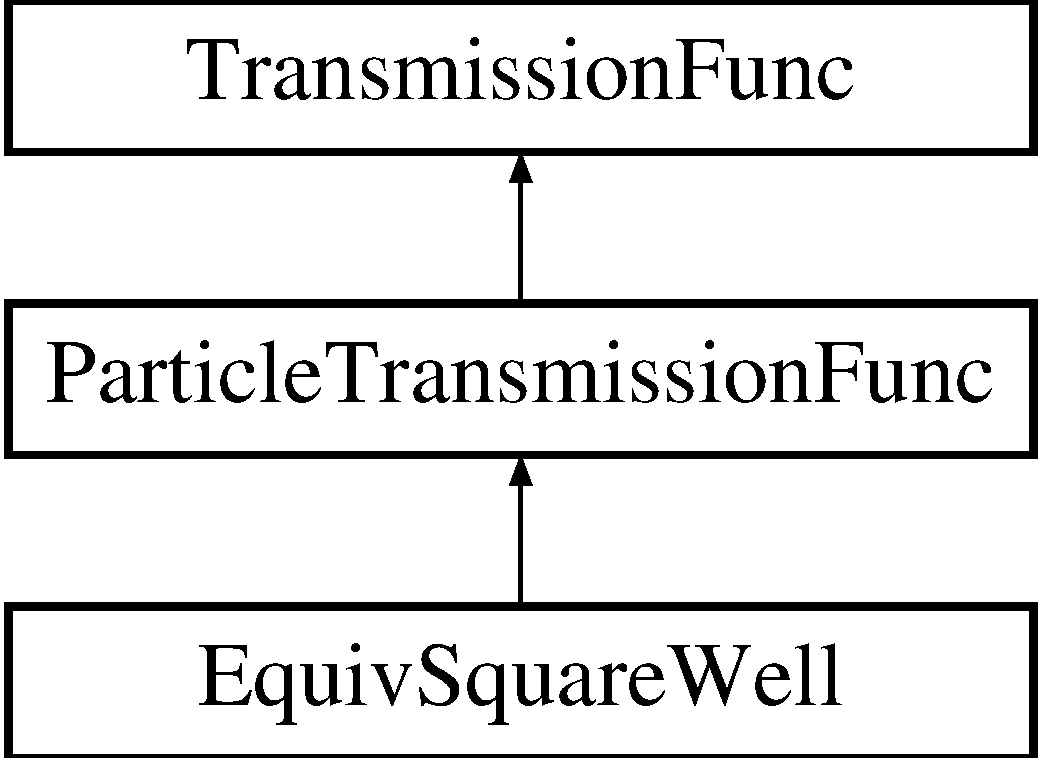
\includegraphics[height=3.000000cm]{d2/d7d/classEquivSquareWell}
\end{center}
\end{figure}
\subsection*{Public Member Functions}
\begin{DoxyCompactItemize}
\item 
\hyperlink{classEquivSquareWell_a234abbef3fc207ade23f1102689ddd01}{Equiv\-Square\-Well} (int z1, int m1, int z2, int m2, double j\-Initial, int pi\-Initial, double j\-Final, int pi\-Final, double spin, int parity, double max\-L, double total\-Width\-For\-Correction, double uncorr\-Total\-Width\-For\-Correction, double uncorr\-Total\-Width\-Sqrd\-For\-Correction, \hyperlink{classTransmissionFunc}{Transmission\-Func} $\ast$previous)
\item 
\hyperlink{classEquivSquareWell_a7a602878ee1afe77d692075ca394caec}{$\sim$\-Equiv\-Square\-Well} ()
\item 
double \hyperlink{classEquivSquareWell_a3b8b7b435b5fcdac36118458ffd5ade8}{Calc\-Transmission} (double, int, double)
\end{DoxyCompactItemize}
\subsection*{Additional Inherited Members}


\subsection{Constructor \& Destructor Documentation}
\hypertarget{classEquivSquareWell_a234abbef3fc207ade23f1102689ddd01}{\index{Equiv\-Square\-Well@{Equiv\-Square\-Well}!Equiv\-Square\-Well@{Equiv\-Square\-Well}}
\index{Equiv\-Square\-Well@{Equiv\-Square\-Well}!EquivSquareWell@{Equiv\-Square\-Well}}
\subsubsection[{Equiv\-Square\-Well}]{\setlength{\rightskip}{0pt plus 5cm}Equiv\-Square\-Well\-::\-Equiv\-Square\-Well (
\begin{DoxyParamCaption}
\item[{int}]{z1, }
\item[{int}]{m1, }
\item[{int}]{z2, }
\item[{int}]{m2, }
\item[{double}]{j\-Initial, }
\item[{int}]{pi\-Initial, }
\item[{double}]{j\-Final, }
\item[{int}]{pi\-Final, }
\item[{double}]{spin, }
\item[{int}]{parity, }
\item[{double}]{max\-L, }
\item[{double}]{total\-Width\-For\-Correction, }
\item[{double}]{uncorr\-Total\-Width\-For\-Correction, }
\item[{double}]{uncorr\-Total\-Width\-Sqrd\-For\-Correction, }
\item[{{\bf Transmission\-Func} $\ast$}]{previous}
\end{DoxyParamCaption}
)\hspace{0.3cm}{\ttfamily [inline]}}}\label{classEquivSquareWell_a234abbef3fc207ade23f1102689ddd01}


References Particle\-Transmission\-Func\-::redmass\-\_\-, Particle\-Transmission\-Func\-::z1\-\_\-, and Transmission\-Func\-::z2\-\_\-.

\hypertarget{classEquivSquareWell_a7a602878ee1afe77d692075ca394caec}{\index{Equiv\-Square\-Well@{Equiv\-Square\-Well}!$\sim$\-Equiv\-Square\-Well@{$\sim$\-Equiv\-Square\-Well}}
\index{$\sim$\-Equiv\-Square\-Well@{$\sim$\-Equiv\-Square\-Well}!EquivSquareWell@{Equiv\-Square\-Well}}
\subsubsection[{$\sim$\-Equiv\-Square\-Well}]{\setlength{\rightskip}{0pt plus 5cm}Equiv\-Square\-Well\-::$\sim$\-Equiv\-Square\-Well (
\begin{DoxyParamCaption}
{}
\end{DoxyParamCaption}
)\hspace{0.3cm}{\ttfamily [inline]}}}\label{classEquivSquareWell_a7a602878ee1afe77d692075ca394caec}


\subsection{Member Function Documentation}
\hypertarget{classEquivSquareWell_a3b8b7b435b5fcdac36118458ffd5ade8}{\index{Equiv\-Square\-Well@{Equiv\-Square\-Well}!Calc\-Transmission@{Calc\-Transmission}}
\index{Calc\-Transmission@{Calc\-Transmission}!EquivSquareWell@{Equiv\-Square\-Well}}
\subsubsection[{Calc\-Transmission}]{\setlength{\rightskip}{0pt plus 5cm}double Equiv\-Square\-Well\-::\-Calc\-Transmission (
\begin{DoxyParamCaption}
\item[{double}]{s, }
\item[{int}]{l, }
\item[{double}]{energy}
\end{DoxyParamCaption}
)\hspace{0.3cm}{\ttfamily [virtual]}}}\label{classEquivSquareWell_a3b8b7b435b5fcdac36118458ffd5ade8}


Implements \hyperlink{classParticleTransmissionFunc_a651cc8a1d96d72e12eaf66506c046856}{Particle\-Transmission\-Func}.



References hbarc, Coul\-Func\-::\-Penetrability(), pi, Particle\-Transmission\-Func\-::redmass\-\_\-, and uconv.



The documentation for this class was generated from the following files\-:\begin{DoxyCompactItemize}
\item 
include/\hyperlink{EquivSquareWell_8h}{Equiv\-Square\-Well.\-h}\item 
src/\hyperlink{EquivSquareWell_8cpp}{Equiv\-Square\-Well.\-cpp}\end{DoxyCompactItemize}

\hypertarget{classGammaTransition}{\section{Gamma\-Transition Class Reference}
\label{classGammaTransition}\index{Gamma\-Transition@{Gamma\-Transition}}
}


{\ttfamily \#include $<$Nuclear\-Levels.\-h$>$}

\subsection*{Public Member Functions}
\begin{DoxyCompactItemize}
\item 
\hyperlink{classGammaTransition_ad6a7e897cbfb83c81d6df5eafeed925d}{Gamma\-Transition} (int level\-Index, double energy, double probability)
\end{DoxyCompactItemize}
\subsection*{Public Attributes}
\begin{DoxyCompactItemize}
\item 
int \hyperlink{classGammaTransition_a021b75eb240faa0a828666d944dd133f}{level\-Index\-\_\-}
\item 
double \hyperlink{classGammaTransition_a548b2d968c5866e6a2ed47755ade3ff4}{energy\-\_\-}
\item 
double \hyperlink{classGammaTransition_a056ef79f20cab353c9b577c720cdf8e4}{probability\-\_\-}
\end{DoxyCompactItemize}


\subsection{Constructor \& Destructor Documentation}
\hypertarget{classGammaTransition_ad6a7e897cbfb83c81d6df5eafeed925d}{\index{Gamma\-Transition@{Gamma\-Transition}!Gamma\-Transition@{Gamma\-Transition}}
\index{Gamma\-Transition@{Gamma\-Transition}!GammaTransition@{Gamma\-Transition}}
\subsubsection[{Gamma\-Transition}]{\setlength{\rightskip}{0pt plus 5cm}Gamma\-Transition\-::\-Gamma\-Transition (
\begin{DoxyParamCaption}
\item[{int}]{level\-Index, }
\item[{double}]{energy, }
\item[{double}]{probability}
\end{DoxyParamCaption}
)\hspace{0.3cm}{\ttfamily [inline]}}}\label{classGammaTransition_ad6a7e897cbfb83c81d6df5eafeed925d}


\subsection{Member Data Documentation}
\hypertarget{classGammaTransition_a548b2d968c5866e6a2ed47755ade3ff4}{\index{Gamma\-Transition@{Gamma\-Transition}!energy\-\_\-@{energy\-\_\-}}
\index{energy\-\_\-@{energy\-\_\-}!GammaTransition@{Gamma\-Transition}}
\subsubsection[{energy\-\_\-}]{\setlength{\rightskip}{0pt plus 5cm}double Gamma\-Transition\-::energy\-\_\-}}\label{classGammaTransition_a548b2d968c5866e6a2ed47755ade3ff4}
\hypertarget{classGammaTransition_a021b75eb240faa0a828666d944dd133f}{\index{Gamma\-Transition@{Gamma\-Transition}!level\-Index\-\_\-@{level\-Index\-\_\-}}
\index{level\-Index\-\_\-@{level\-Index\-\_\-}!GammaTransition@{Gamma\-Transition}}
\subsubsection[{level\-Index\-\_\-}]{\setlength{\rightskip}{0pt plus 5cm}int Gamma\-Transition\-::level\-Index\-\_\-}}\label{classGammaTransition_a021b75eb240faa0a828666d944dd133f}
\hypertarget{classGammaTransition_a056ef79f20cab353c9b577c720cdf8e4}{\index{Gamma\-Transition@{Gamma\-Transition}!probability\-\_\-@{probability\-\_\-}}
\index{probability\-\_\-@{probability\-\_\-}!GammaTransition@{Gamma\-Transition}}
\subsubsection[{probability\-\_\-}]{\setlength{\rightskip}{0pt plus 5cm}double Gamma\-Transition\-::probability\-\_\-}}\label{classGammaTransition_a056ef79f20cab353c9b577c720cdf8e4}


The documentation for this class was generated from the following file\-:\begin{DoxyCompactItemize}
\item 
include/\hyperlink{NuclearLevels_8h}{Nuclear\-Levels.\-h}\end{DoxyCompactItemize}

\hypertarget{classGammaTransmissionFunc}{\section{Gamma\-Transmission\-Func Class Reference}
\label{classGammaTransmissionFunc}\index{Gamma\-Transmission\-Func@{Gamma\-Transmission\-Func}}
}


{\ttfamily \#include $<$Gamma\-Transmission\-Func.\-h$>$}

Inheritance diagram for Gamma\-Transmission\-Func\-:\begin{figure}[H]
\begin{center}
\leavevmode
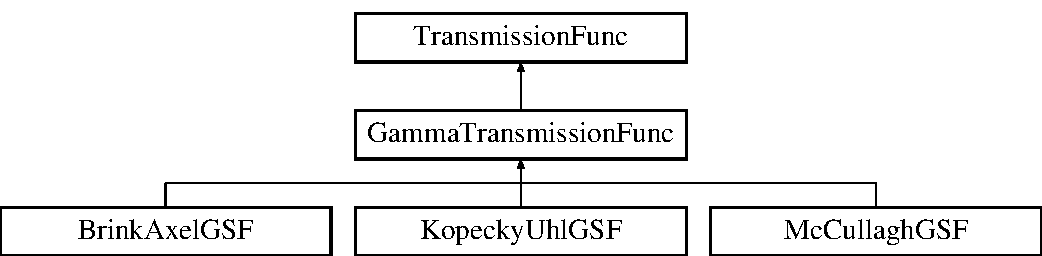
\includegraphics[height=3.000000cm]{dc/d71/classGammaTransmissionFunc}
\end{center}
\end{figure}
\subsection*{Public Member Functions}
\begin{DoxyCompactItemize}
\item 
\hyperlink{classGammaTransmissionFunc_a85c3c4d8857b66b3ba90e63366b550de}{Gamma\-Transmission\-Func} (int, int, double, int, double, int, double, double, double, double, \hyperlink{classTransmissionFunc}{Transmission\-Func} $\ast$)
\item 
virtual \hyperlink{classGammaTransmissionFunc_a5a64da635792941c23cc8eff82b6d235}{$\sim$\-Gamma\-Transmission\-Func} ()
\item 
bool \hyperlink{classGammaTransmissionFunc_aa7947446f3b83320717dd1ca48d48055}{Is\-Valid} ()
\item 
double \hyperlink{classGammaTransmissionFunc_a95be997a9a55e9f56fd00641146ff795}{operator()} (double)
\item 
virtual double \hyperlink{classGammaTransmissionFunc_a68156d72ed9620f66f96dc37bbf781aa}{Calc\-Strength\-Function} (double)=0
\end{DoxyCompactItemize}
\subsection*{Static Public Member Functions}
\begin{DoxyCompactItemize}
\item 
static \hyperlink{classGammaTransmissionFunc}{Gamma\-Transmission\-Func} $\ast$ \hyperlink{classGammaTransmissionFunc_af9113434ffae5b7a9ef26ee4edffa9e2}{Create\-Gamma\-Transmission\-Func} (int, int, double, int, double, int, double, \hyperlink{classLevelDensity}{Level\-Density} $\ast$, double, double, double, \hyperlink{classTransmissionFunc}{Transmission\-Func} $\ast$, double)
\item 
static void \hyperlink{classGammaTransmissionFunc_a2e092550258a4f83308f5177230f9ddd}{Initialize\-G\-D\-R\-Parameters} (std\-::string)
\item 
static void \hyperlink{classGammaTransmissionFunc_a3d7d2c3839a6f793a199d86aa17fcecf}{Set\-E\-G\-D\-R\-Type} (int)
\item 
static void \hyperlink{classGammaTransmissionFunc_ad18fc61af1d1f2f1873072456914d62f}{Set\-Porter\-Thomas} (bool)
\end{DoxyCompactItemize}
\subsection*{Protected Attributes}
\begin{DoxyCompactItemize}
\item 
\hyperlink{classGDRParameters}{G\-D\-R\-Parameters} \hyperlink{classGammaTransmissionFunc_a2fc3e55f03a93237061ef5c72077e007}{gdr\-Parameters\-\_\-}
\end{DoxyCompactItemize}
\subsection*{Static Protected Attributes}
\begin{DoxyCompactItemize}
\item 
static \hyperlink{GammaTransmissionFunc_8h_a28a4ad6d778738bd683db90f04b8c50d}{G\-D\-R\-Table} \hyperlink{classGammaTransmissionFunc_a1ce4515fa2b9343208d5a419b3a8a486}{gdr\-Table\-\_\-}
\item 
static int \hyperlink{classGammaTransmissionFunc_a8cad0e61b388a779ef5dceba294e8687}{egdr\-Type\-\_\-}
\item 
static const int \hyperlink{classGammaTransmissionFunc_ae885f247bb9f13b1ff11aca3626e4069}{mgdr\-Type\-\_\-} =0
\item 
static const int \hyperlink{classGammaTransmissionFunc_a04f3aade1b8c0a2d707fb67028c6fe79}{egqr\-Type\-\_\-} =0
\item 
static bool \hyperlink{classGammaTransmissionFunc_a60dd0efc70eea322e8ca51432418cca2}{porter\-Thomas\-\_\-}
\end{DoxyCompactItemize}


\subsection{Constructor \& Destructor Documentation}
\hypertarget{classGammaTransmissionFunc_a85c3c4d8857b66b3ba90e63366b550de}{\index{Gamma\-Transmission\-Func@{Gamma\-Transmission\-Func}!Gamma\-Transmission\-Func@{Gamma\-Transmission\-Func}}
\index{Gamma\-Transmission\-Func@{Gamma\-Transmission\-Func}!GammaTransmissionFunc@{Gamma\-Transmission\-Func}}
\subsubsection[{Gamma\-Transmission\-Func}]{\setlength{\rightskip}{0pt plus 5cm}Gamma\-Transmission\-Func\-::\-Gamma\-Transmission\-Func (
\begin{DoxyParamCaption}
\item[{int}]{z2, }
\item[{int}]{m2, }
\item[{double}]{j\-Initial, }
\item[{int}]{pi\-Initial, }
\item[{double}]{j\-Final, }
\item[{int}]{pi\-Final, }
\item[{double}]{max\-L, }
\item[{double}]{total\-Width\-For\-Correction, }
\item[{double}]{uncorr\-Total\-Width\-For\-Correction, }
\item[{double}]{uncorr\-Total\-Width\-Sqrd\-For\-Correction, }
\item[{{\bf Transmission\-Func} $\ast$}]{previous}
\end{DoxyParamCaption}
)}}\label{classGammaTransmissionFunc_a85c3c4d8857b66b3ba90e63366b550de}


References Nuclear\-Mass\-::\-Find\-Mass(), fstruc, gdr\-Parameters\-\_\-, gdr\-Table\-\_\-, hbarc, G\-D\-R\-Parameters\-::k\-Sigma\-Gamma\-\_\-, Transmission\-Func\-::m2\-\_\-, pi, and Transmission\-Func\-::z2\-\_\-.

\hypertarget{classGammaTransmissionFunc_a5a64da635792941c23cc8eff82b6d235}{\index{Gamma\-Transmission\-Func@{Gamma\-Transmission\-Func}!$\sim$\-Gamma\-Transmission\-Func@{$\sim$\-Gamma\-Transmission\-Func}}
\index{$\sim$\-Gamma\-Transmission\-Func@{$\sim$\-Gamma\-Transmission\-Func}!GammaTransmissionFunc@{Gamma\-Transmission\-Func}}
\subsubsection[{$\sim$\-Gamma\-Transmission\-Func}]{\setlength{\rightskip}{0pt plus 5cm}virtual Gamma\-Transmission\-Func\-::$\sim$\-Gamma\-Transmission\-Func (
\begin{DoxyParamCaption}
{}
\end{DoxyParamCaption}
)\hspace{0.3cm}{\ttfamily [inline]}, {\ttfamily [virtual]}}}\label{classGammaTransmissionFunc_a5a64da635792941c23cc8eff82b6d235}


\subsection{Member Function Documentation}
\hypertarget{classGammaTransmissionFunc_a68156d72ed9620f66f96dc37bbf781aa}{\index{Gamma\-Transmission\-Func@{Gamma\-Transmission\-Func}!Calc\-Strength\-Function@{Calc\-Strength\-Function}}
\index{Calc\-Strength\-Function@{Calc\-Strength\-Function}!GammaTransmissionFunc@{Gamma\-Transmission\-Func}}
\subsubsection[{Calc\-Strength\-Function}]{\setlength{\rightskip}{0pt plus 5cm}virtual double Gamma\-Transmission\-Func\-::\-Calc\-Strength\-Function (
\begin{DoxyParamCaption}
\item[{double}]{}
\end{DoxyParamCaption}
)\hspace{0.3cm}{\ttfamily [pure virtual]}}}\label{classGammaTransmissionFunc_a68156d72ed9620f66f96dc37bbf781aa}


Implemented in \hyperlink{classBrinkAxelGSF_ac914ac4c34b969ea5b430e07199ed397}{Brink\-Axel\-G\-S\-F}, \hyperlink{classKopeckyUhlGSF_acc719c087bb05ab9cc679c07d887b3ad}{Kopecky\-Uhl\-G\-S\-F}, and \hyperlink{classMcCullaghGSF_ae386ec5251054a5f3a96ee19501bff58}{Mc\-Cullagh\-G\-S\-F}.



Referenced by operator()().

\hypertarget{classGammaTransmissionFunc_af9113434ffae5b7a9ef26ee4edffa9e2}{\index{Gamma\-Transmission\-Func@{Gamma\-Transmission\-Func}!Create\-Gamma\-Transmission\-Func@{Create\-Gamma\-Transmission\-Func}}
\index{Create\-Gamma\-Transmission\-Func@{Create\-Gamma\-Transmission\-Func}!GammaTransmissionFunc@{Gamma\-Transmission\-Func}}
\subsubsection[{Create\-Gamma\-Transmission\-Func}]{\setlength{\rightskip}{0pt plus 5cm}{\bf Gamma\-Transmission\-Func} $\ast$ Gamma\-Transmission\-Func\-::\-Create\-Gamma\-Transmission\-Func (
\begin{DoxyParamCaption}
\item[{int}]{z2, }
\item[{int}]{m2, }
\item[{double}]{j\-Initial, }
\item[{int}]{pi\-Initial, }
\item[{double}]{j\-Final, }
\item[{int}]{pi\-Final, }
\item[{double}]{max\-L, }
\item[{{\bf Level\-Density} $\ast$}]{level\-Density, }
\item[{double}]{total\-Width\-For\-Correction, }
\item[{double}]{uncorr\-Total\-Width\-For\-Correction, }
\item[{double}]{uncorr\-Total\-Width\-Sqrd\-For\-Correction, }
\item[{{\bf Transmission\-Func} $\ast$}]{previous, }
\item[{double}]{compound\-E}
\end{DoxyParamCaption}
)\hspace{0.3cm}{\ttfamily [static]}}}\label{classGammaTransmissionFunc_af9113434ffae5b7a9ef26ee4edffa9e2}


References egdr\-Type\-\_\-, egqr\-Type\-\_\-, and mgdr\-Type\-\_\-.



Referenced by Transition\-Rate\-Func\-::\-Transition\-Rate\-Func().

\hypertarget{classGammaTransmissionFunc_a2e092550258a4f83308f5177230f9ddd}{\index{Gamma\-Transmission\-Func@{Gamma\-Transmission\-Func}!Initialize\-G\-D\-R\-Parameters@{Initialize\-G\-D\-R\-Parameters}}
\index{Initialize\-G\-D\-R\-Parameters@{Initialize\-G\-D\-R\-Parameters}!GammaTransmissionFunc@{Gamma\-Transmission\-Func}}
\subsubsection[{Initialize\-G\-D\-R\-Parameters}]{\setlength{\rightskip}{0pt plus 5cm}void Gamma\-Transmission\-Func\-::\-Initialize\-G\-D\-R\-Parameters (
\begin{DoxyParamCaption}
\item[{std\-::string}]{filename}
\end{DoxyParamCaption}
)\hspace{0.3cm}{\ttfamily [static]}}}\label{classGammaTransmissionFunc_a2e092550258a4f83308f5177230f9ddd}


References gdr\-Table\-\_\-.



Referenced by Initialize().

\hypertarget{classGammaTransmissionFunc_aa7947446f3b83320717dd1ca48d48055}{\index{Gamma\-Transmission\-Func@{Gamma\-Transmission\-Func}!Is\-Valid@{Is\-Valid}}
\index{Is\-Valid@{Is\-Valid}!GammaTransmissionFunc@{Gamma\-Transmission\-Func}}
\subsubsection[{Is\-Valid}]{\setlength{\rightskip}{0pt plus 5cm}bool Gamma\-Transmission\-Func\-::\-Is\-Valid (
\begin{DoxyParamCaption}
{}
\end{DoxyParamCaption}
)\hspace{0.3cm}{\ttfamily [inline]}, {\ttfamily [virtual]}}}\label{classGammaTransmissionFunc_aa7947446f3b83320717dd1ca48d48055}


Implements \hyperlink{classTransmissionFunc_a6dadf2b6cfc37d4c3da0f8ee2a1563af}{Transmission\-Func}.

\hypertarget{classGammaTransmissionFunc_a95be997a9a55e9f56fd00641146ff795}{\index{Gamma\-Transmission\-Func@{Gamma\-Transmission\-Func}!operator()@{operator()}}
\index{operator()@{operator()}!GammaTransmissionFunc@{Gamma\-Transmission\-Func}}
\subsubsection[{operator()}]{\setlength{\rightskip}{0pt plus 5cm}double Gamma\-Transmission\-Func\-::operator() (
\begin{DoxyParamCaption}
\item[{double}]{energy}
\end{DoxyParamCaption}
)\hspace{0.3cm}{\ttfamily [virtual]}}}\label{classGammaTransmissionFunc_a95be997a9a55e9f56fd00641146ff795}


Implements \hyperlink{classTransmissionFunc_ad8df0c8bc498f200ee8b4b95916fe987}{Transmission\-Func}.



References Calc\-Strength\-Function(), Transmission\-Func\-::max\-L\-\_\-, pi, porter\-Thomas\-\_\-, Transmission\-Func\-::previous\-\_\-, random\-Seed, Transmission\-Func\-::total\-Width\-For\-Correction\-\_\-, Transmission\-Func\-::uncorr\-Total\-Width\-For\-Correction\-\_\-, and Transmission\-Func\-::uncorr\-Total\-Width\-Sqrd\-For\-Correction\-\_\-.

\hypertarget{classGammaTransmissionFunc_a3d7d2c3839a6f793a199d86aa17fcecf}{\index{Gamma\-Transmission\-Func@{Gamma\-Transmission\-Func}!Set\-E\-G\-D\-R\-Type@{Set\-E\-G\-D\-R\-Type}}
\index{Set\-E\-G\-D\-R\-Type@{Set\-E\-G\-D\-R\-Type}!GammaTransmissionFunc@{Gamma\-Transmission\-Func}}
\subsubsection[{Set\-E\-G\-D\-R\-Type}]{\setlength{\rightskip}{0pt plus 5cm}void Gamma\-Transmission\-Func\-::\-Set\-E\-G\-D\-R\-Type (
\begin{DoxyParamCaption}
\item[{int}]{type}
\end{DoxyParamCaption}
)\hspace{0.3cm}{\ttfamily [static]}}}\label{classGammaTransmissionFunc_a3d7d2c3839a6f793a199d86aa17fcecf}


References egdr\-Type\-\_\-.



Referenced by Initialize(), and parse\-Command\-Line\-For\-Options().

\hypertarget{classGammaTransmissionFunc_ad18fc61af1d1f2f1873072456914d62f}{\index{Gamma\-Transmission\-Func@{Gamma\-Transmission\-Func}!Set\-Porter\-Thomas@{Set\-Porter\-Thomas}}
\index{Set\-Porter\-Thomas@{Set\-Porter\-Thomas}!GammaTransmissionFunc@{Gamma\-Transmission\-Func}}
\subsubsection[{Set\-Porter\-Thomas}]{\setlength{\rightskip}{0pt plus 5cm}void Gamma\-Transmission\-Func\-::\-Set\-Porter\-Thomas (
\begin{DoxyParamCaption}
\item[{bool}]{yn}
\end{DoxyParamCaption}
)\hspace{0.3cm}{\ttfamily [static]}}}\label{classGammaTransmissionFunc_ad18fc61af1d1f2f1873072456914d62f}


References porter\-Thomas\-\_\-.



Referenced by Initialize(), and parse\-Command\-Line\-For\-Options().



\subsection{Member Data Documentation}
\hypertarget{classGammaTransmissionFunc_a8cad0e61b388a779ef5dceba294e8687}{\index{Gamma\-Transmission\-Func@{Gamma\-Transmission\-Func}!egdr\-Type\-\_\-@{egdr\-Type\-\_\-}}
\index{egdr\-Type\-\_\-@{egdr\-Type\-\_\-}!GammaTransmissionFunc@{Gamma\-Transmission\-Func}}
\subsubsection[{egdr\-Type\-\_\-}]{\setlength{\rightskip}{0pt plus 5cm}int Gamma\-Transmission\-Func\-::egdr\-Type\-\_\-\hspace{0.3cm}{\ttfamily [static]}, {\ttfamily [protected]}}}\label{classGammaTransmissionFunc_a8cad0e61b388a779ef5dceba294e8687}


Referenced by Create\-Gamma\-Transmission\-Func(), and Set\-E\-G\-D\-R\-Type().

\hypertarget{classGammaTransmissionFunc_a04f3aade1b8c0a2d707fb67028c6fe79}{\index{Gamma\-Transmission\-Func@{Gamma\-Transmission\-Func}!egqr\-Type\-\_\-@{egqr\-Type\-\_\-}}
\index{egqr\-Type\-\_\-@{egqr\-Type\-\_\-}!GammaTransmissionFunc@{Gamma\-Transmission\-Func}}
\subsubsection[{egqr\-Type\-\_\-}]{\setlength{\rightskip}{0pt plus 5cm}const int Gamma\-Transmission\-Func\-::egqr\-Type\-\_\- =0\hspace{0.3cm}{\ttfamily [static]}, {\ttfamily [protected]}}}\label{classGammaTransmissionFunc_a04f3aade1b8c0a2d707fb67028c6fe79}


Referenced by Create\-Gamma\-Transmission\-Func().

\hypertarget{classGammaTransmissionFunc_a2fc3e55f03a93237061ef5c72077e007}{\index{Gamma\-Transmission\-Func@{Gamma\-Transmission\-Func}!gdr\-Parameters\-\_\-@{gdr\-Parameters\-\_\-}}
\index{gdr\-Parameters\-\_\-@{gdr\-Parameters\-\_\-}!GammaTransmissionFunc@{Gamma\-Transmission\-Func}}
\subsubsection[{gdr\-Parameters\-\_\-}]{\setlength{\rightskip}{0pt plus 5cm}{\bf G\-D\-R\-Parameters} Gamma\-Transmission\-Func\-::gdr\-Parameters\-\_\-\hspace{0.3cm}{\ttfamily [protected]}}}\label{classGammaTransmissionFunc_a2fc3e55f03a93237061ef5c72077e007}


Referenced by Mc\-Cullagh\-G\-S\-F\-::\-Calc\-Strength\-Function(), Kopecky\-Uhl\-G\-S\-F\-::\-Calc\-Strength\-Function(), Brink\-Axel\-G\-S\-F\-::\-Calc\-Strength\-Function(), and Gamma\-Transmission\-Func().

\hypertarget{classGammaTransmissionFunc_a1ce4515fa2b9343208d5a419b3a8a486}{\index{Gamma\-Transmission\-Func@{Gamma\-Transmission\-Func}!gdr\-Table\-\_\-@{gdr\-Table\-\_\-}}
\index{gdr\-Table\-\_\-@{gdr\-Table\-\_\-}!GammaTransmissionFunc@{Gamma\-Transmission\-Func}}
\subsubsection[{gdr\-Table\-\_\-}]{\setlength{\rightskip}{0pt plus 5cm}{\bf G\-D\-R\-Table} Gamma\-Transmission\-Func\-::gdr\-Table\-\_\-\hspace{0.3cm}{\ttfamily [static]}, {\ttfamily [protected]}}}\label{classGammaTransmissionFunc_a1ce4515fa2b9343208d5a419b3a8a486}


Referenced by Gamma\-Transmission\-Func(), and Initialize\-G\-D\-R\-Parameters().

\hypertarget{classGammaTransmissionFunc_ae885f247bb9f13b1ff11aca3626e4069}{\index{Gamma\-Transmission\-Func@{Gamma\-Transmission\-Func}!mgdr\-Type\-\_\-@{mgdr\-Type\-\_\-}}
\index{mgdr\-Type\-\_\-@{mgdr\-Type\-\_\-}!GammaTransmissionFunc@{Gamma\-Transmission\-Func}}
\subsubsection[{mgdr\-Type\-\_\-}]{\setlength{\rightskip}{0pt plus 5cm}const int Gamma\-Transmission\-Func\-::mgdr\-Type\-\_\- =0\hspace{0.3cm}{\ttfamily [static]}, {\ttfamily [protected]}}}\label{classGammaTransmissionFunc_ae885f247bb9f13b1ff11aca3626e4069}


Referenced by Create\-Gamma\-Transmission\-Func().

\hypertarget{classGammaTransmissionFunc_a60dd0efc70eea322e8ca51432418cca2}{\index{Gamma\-Transmission\-Func@{Gamma\-Transmission\-Func}!porter\-Thomas\-\_\-@{porter\-Thomas\-\_\-}}
\index{porter\-Thomas\-\_\-@{porter\-Thomas\-\_\-}!GammaTransmissionFunc@{Gamma\-Transmission\-Func}}
\subsubsection[{porter\-Thomas\-\_\-}]{\setlength{\rightskip}{0pt plus 5cm}bool Gamma\-Transmission\-Func\-::porter\-Thomas\-\_\-\hspace{0.3cm}{\ttfamily [static]}, {\ttfamily [protected]}}}\label{classGammaTransmissionFunc_a60dd0efc70eea322e8ca51432418cca2}


Referenced by operator()(), and Set\-Porter\-Thomas().



The documentation for this class was generated from the following files\-:\begin{DoxyCompactItemize}
\item 
include/\hyperlink{GammaTransmissionFunc_8h}{Gamma\-Transmission\-Func.\-h}\item 
src/\hyperlink{GammaTransmissionFunc_8cpp}{Gamma\-Transmission\-Func.\-cpp}\item 
src/\hyperlink{Setup_8cpp}{Setup.\-cpp}\end{DoxyCompactItemize}

\hypertarget{classGDRParameters}{\section{G\-D\-R\-Parameters Class Reference}
\label{classGDRParameters}\index{G\-D\-R\-Parameters@{G\-D\-R\-Parameters}}
}


{\ttfamily \#include $<$Gamma\-Transmission\-Func.\-h$>$}

\subsection*{Public Member Functions}
\begin{DoxyCompactItemize}
\item 
\hyperlink{classGDRParameters_af6a2e57fc9e118d77bf7ae0fa0e9abea}{G\-D\-R\-Parameters} ()
\item 
\hyperlink{classGDRParameters_a6a4f96227c922ddccfe0307e89bf1358}{G\-D\-R\-Parameters} (double eta, double E1, double W1, double k\-Sigma\-Gamma1, double E2, double W2, double k\-Sigma\-Gamma2)
\end{DoxyCompactItemize}
\subsection*{Public Attributes}
\begin{DoxyCompactItemize}
\item 
double \hyperlink{classGDRParameters_ad934d0d1a4a3ad93326f9af97eeb9d7c}{eta\-\_\-}
\item 
double \hyperlink{classGDRParameters_a3a02ecbe435e6ac419eaeace7be0ac3b}{E\-\_\-} \mbox{[}2\mbox{]}
\item 
double \hyperlink{classGDRParameters_ab907ef31caef7af38a2ed6bc8a45e365}{W\-\_\-} \mbox{[}2\mbox{]}
\item 
double \hyperlink{classGDRParameters_afd7899667da29eab4842a6e1389b3386}{k\-Sigma\-Gamma\-\_\-} \mbox{[}2\mbox{]}
\end{DoxyCompactItemize}


\subsection{Constructor \& Destructor Documentation}
\hypertarget{classGDRParameters_af6a2e57fc9e118d77bf7ae0fa0e9abea}{\index{G\-D\-R\-Parameters@{G\-D\-R\-Parameters}!G\-D\-R\-Parameters@{G\-D\-R\-Parameters}}
\index{G\-D\-R\-Parameters@{G\-D\-R\-Parameters}!GDRParameters@{G\-D\-R\-Parameters}}
\subsubsection[{G\-D\-R\-Parameters}]{\setlength{\rightskip}{0pt plus 5cm}G\-D\-R\-Parameters\-::\-G\-D\-R\-Parameters (
\begin{DoxyParamCaption}
{}
\end{DoxyParamCaption}
)\hspace{0.3cm}{\ttfamily [inline]}}}\label{classGDRParameters_af6a2e57fc9e118d77bf7ae0fa0e9abea}


References E\-\_\-, and W\-\_\-.

\hypertarget{classGDRParameters_a6a4f96227c922ddccfe0307e89bf1358}{\index{G\-D\-R\-Parameters@{G\-D\-R\-Parameters}!G\-D\-R\-Parameters@{G\-D\-R\-Parameters}}
\index{G\-D\-R\-Parameters@{G\-D\-R\-Parameters}!GDRParameters@{G\-D\-R\-Parameters}}
\subsubsection[{G\-D\-R\-Parameters}]{\setlength{\rightskip}{0pt plus 5cm}G\-D\-R\-Parameters\-::\-G\-D\-R\-Parameters (
\begin{DoxyParamCaption}
\item[{double}]{eta, }
\item[{double}]{E1, }
\item[{double}]{W1, }
\item[{double}]{k\-Sigma\-Gamma1, }
\item[{double}]{E2, }
\item[{double}]{W2, }
\item[{double}]{k\-Sigma\-Gamma2}
\end{DoxyParamCaption}
)\hspace{0.3cm}{\ttfamily [inline]}}}\label{classGDRParameters_a6a4f96227c922ddccfe0307e89bf1358}


References E\-\_\-, k\-Sigma\-Gamma\-\_\-, and W\-\_\-.



\subsection{Member Data Documentation}
\hypertarget{classGDRParameters_a3a02ecbe435e6ac419eaeace7be0ac3b}{\index{G\-D\-R\-Parameters@{G\-D\-R\-Parameters}!E\-\_\-@{E\-\_\-}}
\index{E\-\_\-@{E\-\_\-}!GDRParameters@{G\-D\-R\-Parameters}}
\subsubsection[{E\-\_\-}]{\setlength{\rightskip}{0pt plus 5cm}double G\-D\-R\-Parameters\-::\-E\-\_\-\mbox{[}2\mbox{]}}}\label{classGDRParameters_a3a02ecbe435e6ac419eaeace7be0ac3b}


Referenced by Mc\-Cullagh\-G\-S\-F\-::\-Calc\-Strength\-Function(), Kopecky\-Uhl\-G\-S\-F\-::\-Calc\-Strength\-Function(), Brink\-Axel\-G\-S\-F\-::\-Calc\-Strength\-Function(), and G\-D\-R\-Parameters().

\hypertarget{classGDRParameters_ad934d0d1a4a3ad93326f9af97eeb9d7c}{\index{G\-D\-R\-Parameters@{G\-D\-R\-Parameters}!eta\-\_\-@{eta\-\_\-}}
\index{eta\-\_\-@{eta\-\_\-}!GDRParameters@{G\-D\-R\-Parameters}}
\subsubsection[{eta\-\_\-}]{\setlength{\rightskip}{0pt plus 5cm}double G\-D\-R\-Parameters\-::eta\-\_\-}}\label{classGDRParameters_ad934d0d1a4a3ad93326f9af97eeb9d7c}
\hypertarget{classGDRParameters_afd7899667da29eab4842a6e1389b3386}{\index{G\-D\-R\-Parameters@{G\-D\-R\-Parameters}!k\-Sigma\-Gamma\-\_\-@{k\-Sigma\-Gamma\-\_\-}}
\index{k\-Sigma\-Gamma\-\_\-@{k\-Sigma\-Gamma\-\_\-}!GDRParameters@{G\-D\-R\-Parameters}}
\subsubsection[{k\-Sigma\-Gamma\-\_\-}]{\setlength{\rightskip}{0pt plus 5cm}double G\-D\-R\-Parameters\-::k\-Sigma\-Gamma\-\_\-\mbox{[}2\mbox{]}}}\label{classGDRParameters_afd7899667da29eab4842a6e1389b3386}


Referenced by Mc\-Cullagh\-G\-S\-F\-::\-Calc\-Strength\-Function(), Kopecky\-Uhl\-G\-S\-F\-::\-Calc\-Strength\-Function(), Brink\-Axel\-G\-S\-F\-::\-Calc\-Strength\-Function(), Gamma\-Transmission\-Func\-::\-Gamma\-Transmission\-Func(), and G\-D\-R\-Parameters().

\hypertarget{classGDRParameters_ab907ef31caef7af38a2ed6bc8a45e365}{\index{G\-D\-R\-Parameters@{G\-D\-R\-Parameters}!W\-\_\-@{W\-\_\-}}
\index{W\-\_\-@{W\-\_\-}!GDRParameters@{G\-D\-R\-Parameters}}
\subsubsection[{W\-\_\-}]{\setlength{\rightskip}{0pt plus 5cm}double G\-D\-R\-Parameters\-::\-W\-\_\-\mbox{[}2\mbox{]}}}\label{classGDRParameters_ab907ef31caef7af38a2ed6bc8a45e365}


Referenced by Kopecky\-Uhl\-G\-S\-F\-::\-Calc\-Strength\-Function(), and G\-D\-R\-Parameters().



The documentation for this class was generated from the following file\-:\begin{DoxyCompactItemize}
\item 
include/\hyperlink{GammaTransmissionFunc_8h}{Gamma\-Transmission\-Func.\-h}\end{DoxyCompactItemize}

\hypertarget{structgsl__partfunc__params}{\section{gsl\-\_\-partfunc\-\_\-params Struct Reference}
\label{structgsl__partfunc__params}\index{gsl\-\_\-partfunc\-\_\-params@{gsl\-\_\-partfunc\-\_\-params}}
}
\subsection*{Public Attributes}
\begin{DoxyCompactItemize}
\item 
double \hyperlink{structgsl__partfunc__params_ae8330967c4990a3497f423816f9ccccf}{temperature}
\item 
\hyperlink{classLevelDensity}{Level\-Density} $\ast$ \hyperlink{structgsl__partfunc__params_adbaf4c10b4af6cc003d74c80895ebfb8}{density}
\end{DoxyCompactItemize}


\subsection{Member Data Documentation}
\hypertarget{structgsl__partfunc__params_adbaf4c10b4af6cc003d74c80895ebfb8}{\index{gsl\-\_\-partfunc\-\_\-params@{gsl\-\_\-partfunc\-\_\-params}!density@{density}}
\index{density@{density}!gsl_partfunc_params@{gsl\-\_\-partfunc\-\_\-params}}
\subsubsection[{density}]{\setlength{\rightskip}{0pt plus 5cm}{\bf Level\-Density}$\ast$ gsl\-\_\-partfunc\-\_\-params\-::density}}\label{structgsl__partfunc__params_adbaf4c10b4af6cc003d74c80895ebfb8}


Referenced by gsl\-\_\-partfunc\-\_\-integrand(), Level\-Density\-::operator()(), and Level\-Density\-::\-Total\-Level\-Density().

\hypertarget{structgsl__partfunc__params_ae8330967c4990a3497f423816f9ccccf}{\index{gsl\-\_\-partfunc\-\_\-params@{gsl\-\_\-partfunc\-\_\-params}!temperature@{temperature}}
\index{temperature@{temperature}!gsl_partfunc_params@{gsl\-\_\-partfunc\-\_\-params}}
\subsubsection[{temperature}]{\setlength{\rightskip}{0pt plus 5cm}double gsl\-\_\-partfunc\-\_\-params\-::temperature}}\label{structgsl__partfunc__params_ae8330967c4990a3497f423816f9ccccf}


Referenced by gsl\-\_\-partfunc\-\_\-integrand().



The documentation for this struct was generated from the following file\-:\begin{DoxyCompactItemize}
\item 
src/\hyperlink{CrossSection_8cpp}{Cross\-Section.\-cpp}\end{DoxyCompactItemize}

\hypertarget{structgsl__reactionrate__params}{\section{gsl\-\_\-reactionrate\-\_\-params Struct Reference}
\label{structgsl__reactionrate__params}\index{gsl\-\_\-reactionrate\-\_\-params@{gsl\-\_\-reactionrate\-\_\-params}}
}
\subsection*{Public Attributes}
\begin{DoxyCompactItemize}
\item 
double \hyperlink{structgsl__reactionrate__params_a207cb264645c40bd2cbac28328e8c48f}{temperature}
\item 
T\-Graph $\ast$ \hyperlink{structgsl__reactionrate__params_a58f7496d7c40bbb4df13305ba1ed0c77}{graph}
\item 
bool \hyperlink{structgsl__reactionrate__params_ac8d064fc50f87de0d067926ba0f2abb7}{use\-Spline}
\end{DoxyCompactItemize}


\subsection{Member Data Documentation}
\hypertarget{structgsl__reactionrate__params_a58f7496d7c40bbb4df13305ba1ed0c77}{\index{gsl\-\_\-reactionrate\-\_\-params@{gsl\-\_\-reactionrate\-\_\-params}!graph@{graph}}
\index{graph@{graph}!gsl_reactionrate_params@{gsl\-\_\-reactionrate\-\_\-params}}
\subsubsection[{graph}]{\setlength{\rightskip}{0pt plus 5cm}T\-Graph$\ast$ gsl\-\_\-reactionrate\-\_\-params\-::graph}}\label{structgsl__reactionrate__params_a58f7496d7c40bbb4df13305ba1ed0c77}


Referenced by gsl\-\_\-reactionrate\-\_\-integrand().

\hypertarget{structgsl__reactionrate__params_a207cb264645c40bd2cbac28328e8c48f}{\index{gsl\-\_\-reactionrate\-\_\-params@{gsl\-\_\-reactionrate\-\_\-params}!temperature@{temperature}}
\index{temperature@{temperature}!gsl_reactionrate_params@{gsl\-\_\-reactionrate\-\_\-params}}
\subsubsection[{temperature}]{\setlength{\rightskip}{0pt plus 5cm}double gsl\-\_\-reactionrate\-\_\-params\-::temperature}}\label{structgsl__reactionrate__params_a207cb264645c40bd2cbac28328e8c48f}


Referenced by gsl\-\_\-reactionrate\-\_\-integrand().

\hypertarget{structgsl__reactionrate__params_ac8d064fc50f87de0d067926ba0f2abb7}{\index{gsl\-\_\-reactionrate\-\_\-params@{gsl\-\_\-reactionrate\-\_\-params}!use\-Spline@{use\-Spline}}
\index{use\-Spline@{use\-Spline}!gsl_reactionrate_params@{gsl\-\_\-reactionrate\-\_\-params}}
\subsubsection[{use\-Spline}]{\setlength{\rightskip}{0pt plus 5cm}bool gsl\-\_\-reactionrate\-\_\-params\-::use\-Spline}}\label{structgsl__reactionrate__params_ac8d064fc50f87de0d067926ba0f2abb7}


Referenced by gsl\-\_\-reactionrate\-\_\-integrand().



The documentation for this struct was generated from the following file\-:\begin{DoxyCompactItemize}
\item 
src/\hyperlink{CrossSection_8cpp}{Cross\-Section.\-cpp}\end{DoxyCompactItemize}

\hypertarget{structstd_1_1tr1_1_1hash_3_01MassKey_01_4}{\section{std\-:\-:tr1\-:\-:hash$<$ Mass\-Key $>$ Struct Template Reference}
\label{structstd_1_1tr1_1_1hash_3_01MassKey_01_4}\index{std\-::tr1\-::hash$<$ Mass\-Key $>$@{std\-::tr1\-::hash$<$ Mass\-Key $>$}}
}


{\ttfamily \#include $<$Nuclear\-Mass.\-h$>$}

\subsection*{Public Member Functions}
\begin{DoxyCompactItemize}
\item 
std\-::size\-\_\-t \hyperlink{structstd_1_1tr1_1_1hash_3_01MassKey_01_4_a2c6d1568039949a867568b13b5c41af0}{operator()} (\hyperlink{classMassKey}{Mass\-Key} const \&key) const 
\end{DoxyCompactItemize}


\subsection{Member Function Documentation}
\hypertarget{structstd_1_1tr1_1_1hash_3_01MassKey_01_4_a2c6d1568039949a867568b13b5c41af0}{\index{std\-::tr1\-::hash$<$ Mass\-Key $>$@{std\-::tr1\-::hash$<$ Mass\-Key $>$}!operator()@{operator()}}
\index{operator()@{operator()}!std::tr1::hash< MassKey >@{std\-::tr1\-::hash$<$ Mass\-Key $>$}}
\subsubsection[{operator()}]{\setlength{\rightskip}{0pt plus 5cm}std\-::size\-\_\-t std\-::tr1\-::hash$<$ {\bf Mass\-Key} $>$\-::operator() (
\begin{DoxyParamCaption}
\item[{{\bf Mass\-Key} const \&}]{key}
\end{DoxyParamCaption}
) const\hspace{0.3cm}{\ttfamily [inline]}}}\label{structstd_1_1tr1_1_1hash_3_01MassKey_01_4_a2c6d1568039949a867568b13b5c41af0}


References Mass\-Key\-::\-A\-\_\-, and Mass\-Key\-::\-Z\-\_\-.



The documentation for this struct was generated from the following file\-:\begin{DoxyCompactItemize}
\item 
/afs/crc.\-nd.\-edu/user/p/pscholz/\-Private/sapphire-\/devel/include/\hyperlink{NuclearMass_8h}{Nuclear\-Mass.\-h}\end{DoxyCompactItemize}

\hypertarget{classInitialNucleusData}{\section{Initial\-Nucleus\-Data Class Reference}
\label{classInitialNucleusData}\index{Initial\-Nucleus\-Data@{Initial\-Nucleus\-Data}}
}


{\ttfamily \#include $<$Sapphire\-M\-P\-I\-Types.\-h$>$}

\subsection*{Public Member Functions}
\begin{DoxyCompactItemize}
\item 
\hyperlink{classInitialNucleusData_a8654c0d1ade76565b56a6623b6629307}{Initial\-Nucleus\-Data} ()
\item 
\hyperlink{classInitialNucleusData_a4b2b8485eb4c335278c39ed77bd02487}{Initial\-Nucleus\-Data} (int \hyperlink{classInitialNucleusData_a1ee1ed6bc4ea256f93bfd9bd9a0b96c6}{Z}, int \hyperlink{classInitialNucleusData_a4dec3fe9a44e5142de89c28bef45dbe0}{A}, double \hyperlink{classInitialNucleusData_ae2400790c869bdea1e1f79619dff7157}{J}, int \hyperlink{classInitialNucleusData_ad63e3dad51fa52a88477b97437841628}{Pi}, double \hyperlink{classInitialNucleusData_abe498b5aadeb835836cf7be4211ba227}{low\-Energy}, double \hyperlink{classInitialNucleusData_ab4ce2ac971e5c34748bdb826ec42d121}{high\-Energy}, bool \hyperlink{classInitialNucleusData_a15b4c0e140550e3c4be67b615a832cfa}{pre\-Eq})
\item 
bool \hyperlink{classInitialNucleusData_a15b4c0e140550e3c4be67b615a832cfa}{pre\-Eq} () const 
\item 
int \hyperlink{classInitialNucleusData_a1ee1ed6bc4ea256f93bfd9bd9a0b96c6}{Z} () const 
\item 
int \hyperlink{classInitialNucleusData_a4dec3fe9a44e5142de89c28bef45dbe0}{A} () const 
\item 
int \hyperlink{classInitialNucleusData_ad63e3dad51fa52a88477b97437841628}{Pi} () const 
\item 
double \hyperlink{classInitialNucleusData_ae2400790c869bdea1e1f79619dff7157}{J} () const 
\item 
double \hyperlink{classInitialNucleusData_abe498b5aadeb835836cf7be4211ba227}{low\-Energy} () const 
\item 
double \hyperlink{classInitialNucleusData_ab4ce2ac971e5c34748bdb826ec42d121}{high\-Energy} () const 
\end{DoxyCompactItemize}
\subsection*{Friends}
\begin{DoxyCompactItemize}
\item 
class \hyperlink{classInitialNucleusData_ac98d07dd8f7b70e16ccb9a01abf56b9c}{boost\-::serialization\-::access}
\end{DoxyCompactItemize}


\subsection{Constructor \& Destructor Documentation}
\hypertarget{classInitialNucleusData_a8654c0d1ade76565b56a6623b6629307}{\index{Initial\-Nucleus\-Data@{Initial\-Nucleus\-Data}!Initial\-Nucleus\-Data@{Initial\-Nucleus\-Data}}
\index{Initial\-Nucleus\-Data@{Initial\-Nucleus\-Data}!InitialNucleusData@{Initial\-Nucleus\-Data}}
\subsubsection[{Initial\-Nucleus\-Data}]{\setlength{\rightskip}{0pt plus 5cm}Initial\-Nucleus\-Data\-::\-Initial\-Nucleus\-Data (
\begin{DoxyParamCaption}
{}
\end{DoxyParamCaption}
)\hspace{0.3cm}{\ttfamily [inline]}}}\label{classInitialNucleusData_a8654c0d1ade76565b56a6623b6629307}
\hypertarget{classInitialNucleusData_a4b2b8485eb4c335278c39ed77bd02487}{\index{Initial\-Nucleus\-Data@{Initial\-Nucleus\-Data}!Initial\-Nucleus\-Data@{Initial\-Nucleus\-Data}}
\index{Initial\-Nucleus\-Data@{Initial\-Nucleus\-Data}!InitialNucleusData@{Initial\-Nucleus\-Data}}
\subsubsection[{Initial\-Nucleus\-Data}]{\setlength{\rightskip}{0pt plus 5cm}Initial\-Nucleus\-Data\-::\-Initial\-Nucleus\-Data (
\begin{DoxyParamCaption}
\item[{int}]{Z, }
\item[{int}]{A, }
\item[{double}]{J, }
\item[{int}]{Pi, }
\item[{double}]{low\-Energy, }
\item[{double}]{high\-Energy, }
\item[{bool}]{pre\-Eq}
\end{DoxyParamCaption}
)\hspace{0.3cm}{\ttfamily [inline]}}}\label{classInitialNucleusData_a4b2b8485eb4c335278c39ed77bd02487}


\subsection{Member Function Documentation}
\hypertarget{classInitialNucleusData_a4dec3fe9a44e5142de89c28bef45dbe0}{\index{Initial\-Nucleus\-Data@{Initial\-Nucleus\-Data}!A@{A}}
\index{A@{A}!InitialNucleusData@{Initial\-Nucleus\-Data}}
\subsubsection[{A}]{\setlength{\rightskip}{0pt plus 5cm}int Initial\-Nucleus\-Data\-::\-A (
\begin{DoxyParamCaption}
{}
\end{DoxyParamCaption}
) const\hspace{0.3cm}{\ttfamily [inline]}}}\label{classInitialNucleusData_a4dec3fe9a44e5142de89c28bef45dbe0}
\hypertarget{classInitialNucleusData_ab4ce2ac971e5c34748bdb826ec42d121}{\index{Initial\-Nucleus\-Data@{Initial\-Nucleus\-Data}!high\-Energy@{high\-Energy}}
\index{high\-Energy@{high\-Energy}!InitialNucleusData@{Initial\-Nucleus\-Data}}
\subsubsection[{high\-Energy}]{\setlength{\rightskip}{0pt plus 5cm}double Initial\-Nucleus\-Data\-::high\-Energy (
\begin{DoxyParamCaption}
{}
\end{DoxyParamCaption}
) const\hspace{0.3cm}{\ttfamily [inline]}}}\label{classInitialNucleusData_ab4ce2ac971e5c34748bdb826ec42d121}
\hypertarget{classInitialNucleusData_ae2400790c869bdea1e1f79619dff7157}{\index{Initial\-Nucleus\-Data@{Initial\-Nucleus\-Data}!J@{J}}
\index{J@{J}!InitialNucleusData@{Initial\-Nucleus\-Data}}
\subsubsection[{J}]{\setlength{\rightskip}{0pt plus 5cm}double Initial\-Nucleus\-Data\-::\-J (
\begin{DoxyParamCaption}
{}
\end{DoxyParamCaption}
) const\hspace{0.3cm}{\ttfamily [inline]}}}\label{classInitialNucleusData_ae2400790c869bdea1e1f79619dff7157}
\hypertarget{classInitialNucleusData_abe498b5aadeb835836cf7be4211ba227}{\index{Initial\-Nucleus\-Data@{Initial\-Nucleus\-Data}!low\-Energy@{low\-Energy}}
\index{low\-Energy@{low\-Energy}!InitialNucleusData@{Initial\-Nucleus\-Data}}
\subsubsection[{low\-Energy}]{\setlength{\rightskip}{0pt plus 5cm}double Initial\-Nucleus\-Data\-::low\-Energy (
\begin{DoxyParamCaption}
{}
\end{DoxyParamCaption}
) const\hspace{0.3cm}{\ttfamily [inline]}}}\label{classInitialNucleusData_abe498b5aadeb835836cf7be4211ba227}
\hypertarget{classInitialNucleusData_ad63e3dad51fa52a88477b97437841628}{\index{Initial\-Nucleus\-Data@{Initial\-Nucleus\-Data}!Pi@{Pi}}
\index{Pi@{Pi}!InitialNucleusData@{Initial\-Nucleus\-Data}}
\subsubsection[{Pi}]{\setlength{\rightskip}{0pt plus 5cm}int Initial\-Nucleus\-Data\-::\-Pi (
\begin{DoxyParamCaption}
{}
\end{DoxyParamCaption}
) const\hspace{0.3cm}{\ttfamily [inline]}}}\label{classInitialNucleusData_ad63e3dad51fa52a88477b97437841628}
\hypertarget{classInitialNucleusData_a15b4c0e140550e3c4be67b615a832cfa}{\index{Initial\-Nucleus\-Data@{Initial\-Nucleus\-Data}!pre\-Eq@{pre\-Eq}}
\index{pre\-Eq@{pre\-Eq}!InitialNucleusData@{Initial\-Nucleus\-Data}}
\subsubsection[{pre\-Eq}]{\setlength{\rightskip}{0pt plus 5cm}bool Initial\-Nucleus\-Data\-::pre\-Eq (
\begin{DoxyParamCaption}
{}
\end{DoxyParamCaption}
) const\hspace{0.3cm}{\ttfamily [inline]}}}\label{classInitialNucleusData_a15b4c0e140550e3c4be67b615a832cfa}
\hypertarget{classInitialNucleusData_a1ee1ed6bc4ea256f93bfd9bd9a0b96c6}{\index{Initial\-Nucleus\-Data@{Initial\-Nucleus\-Data}!Z@{Z}}
\index{Z@{Z}!InitialNucleusData@{Initial\-Nucleus\-Data}}
\subsubsection[{Z}]{\setlength{\rightskip}{0pt plus 5cm}int Initial\-Nucleus\-Data\-::\-Z (
\begin{DoxyParamCaption}
{}
\end{DoxyParamCaption}
) const\hspace{0.3cm}{\ttfamily [inline]}}}\label{classInitialNucleusData_a1ee1ed6bc4ea256f93bfd9bd9a0b96c6}


\subsection{Friends And Related Function Documentation}
\hypertarget{classInitialNucleusData_ac98d07dd8f7b70e16ccb9a01abf56b9c}{\index{Initial\-Nucleus\-Data@{Initial\-Nucleus\-Data}!boost\-::serialization\-::access@{boost\-::serialization\-::access}}
\index{boost\-::serialization\-::access@{boost\-::serialization\-::access}!InitialNucleusData@{Initial\-Nucleus\-Data}}
\subsubsection[{boost\-::serialization\-::access}]{\setlength{\rightskip}{0pt plus 5cm}friend class boost\-::serialization\-::access\hspace{0.3cm}{\ttfamily [friend]}}}\label{classInitialNucleusData_ac98d07dd8f7b70e16ccb9a01abf56b9c}


The documentation for this class was generated from the following file\-:\begin{DoxyCompactItemize}
\item 
include/\hyperlink{SapphireMPITypes_8h}{Sapphire\-M\-P\-I\-Types.\-h}\end{DoxyCompactItemize}

\hypertarget{structint__double__pair__compare}{\section{int\-\_\-double\-\_\-pair\-\_\-compare Struct Reference}
\label{structint__double__pair__compare}\index{int\-\_\-double\-\_\-pair\-\_\-compare@{int\-\_\-double\-\_\-pair\-\_\-compare}}
}


{\ttfamily \#include $<$Cross\-Section.\-h$>$}

\subsection*{Public Member Functions}
\begin{DoxyCompactItemize}
\item 
bool \hyperlink{structint__double__pair__compare_ab44e2aa41f673738ab1a143a722141c5}{operator()} (const \hyperlink{CrossSection_8h_a86977dc16e076fab82d0ed0b04070c96}{int\-\_\-double\-\_\-pair} \&lhs, \hyperlink{CrossSection_8h_a86977dc16e076fab82d0ed0b04070c96}{int\-\_\-double\-\_\-pair} const \&rhs)
\end{DoxyCompactItemize}


\subsection{Member Function Documentation}
\hypertarget{structint__double__pair__compare_ab44e2aa41f673738ab1a143a722141c5}{\index{int\-\_\-double\-\_\-pair\-\_\-compare@{int\-\_\-double\-\_\-pair\-\_\-compare}!operator()@{operator()}}
\index{operator()@{operator()}!int_double_pair_compare@{int\-\_\-double\-\_\-pair\-\_\-compare}}
\subsubsection[{operator()}]{\setlength{\rightskip}{0pt plus 5cm}bool int\-\_\-double\-\_\-pair\-\_\-compare\-::operator() (
\begin{DoxyParamCaption}
\item[{const {\bf int\-\_\-double\-\_\-pair} \&}]{lhs, }
\item[{{\bf int\-\_\-double\-\_\-pair} const \&}]{rhs}
\end{DoxyParamCaption}
)\hspace{0.3cm}{\ttfamily [inline]}}}\label{structint__double__pair__compare_ab44e2aa41f673738ab1a143a722141c5}


The documentation for this struct was generated from the following file\-:\begin{DoxyCompactItemize}
\item 
include/\hyperlink{CrossSection_8h}{Cross\-Section.\-h}\end{DoxyCompactItemize}

\hypertarget{classJLMPotential}{\section{J\-L\-M\-Potential Class Reference}
\label{classJLMPotential}\index{J\-L\-M\-Potential@{J\-L\-M\-Potential}}
}


{\ttfamily \#include $<$J\-L\-M\-Potential.\-h$>$}

Inheritance diagram for J\-L\-M\-Potential\-:\begin{figure}[H]
\begin{center}
\leavevmode
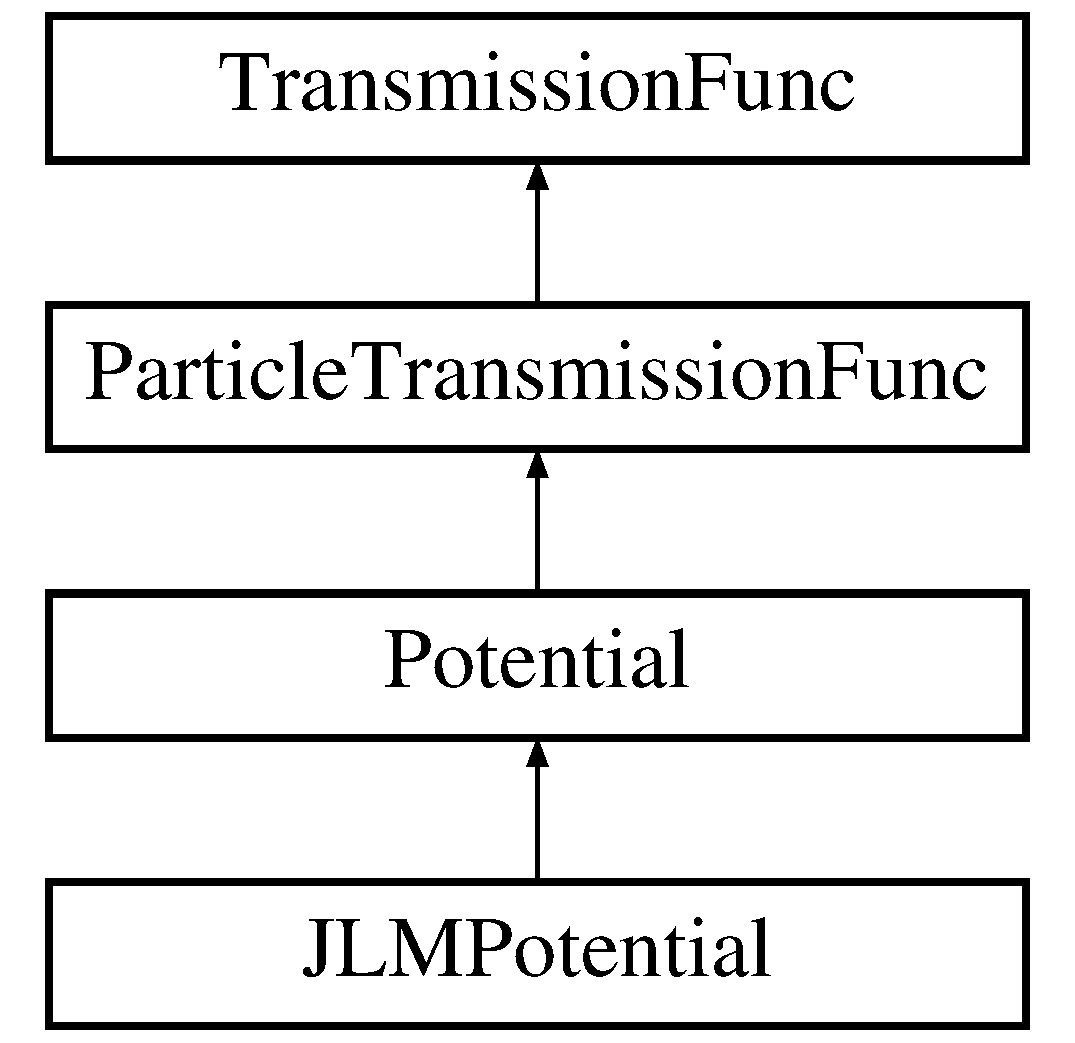
\includegraphics[height=4.000000cm]{dc/d98/classJLMPotential}
\end{center}
\end{figure}
\subsection*{Public Member Functions}
\begin{DoxyCompactItemize}
\item 
\hyperlink{classJLMPotential_a60af1fcc741ca4bb457160093a4d4149}{J\-L\-M\-Potential} (int, int, int, int, double, int, double, int, double, int, double, double, double, double, \hyperlink{classTransmissionFunc}{Transmission\-Func} $\ast$)
\item 
double \hyperlink{classJLMPotential_afb78b10d84a5454e68c7e1a558662c7f}{Calculate\-Density} (double, int) const 
\item 
\hyperlink{Constants_8h_a1c1b16cc02d518bbe753449171ab7033}{std\-::complex}$<$ double $>$ \hyperlink{classJLMPotential_ae9986807ce14a95a6c6214feea1233c8}{Calculate} (double, int, double, double, double) const 
\end{DoxyCompactItemize}
\subsection*{Static Public Member Functions}
\begin{DoxyCompactItemize}
\item 
static double \hyperlink{classJLMPotential_af8abb42c2334e41bd726a4fb44c05568}{Get\-A} (int i, int j)
\end{DoxyCompactItemize}
\subsection*{Additional Inherited Members}


\subsection{Constructor \& Destructor Documentation}
\hypertarget{classJLMPotential_a60af1fcc741ca4bb457160093a4d4149}{\index{J\-L\-M\-Potential@{J\-L\-M\-Potential}!J\-L\-M\-Potential@{J\-L\-M\-Potential}}
\index{J\-L\-M\-Potential@{J\-L\-M\-Potential}!JLMPotential@{J\-L\-M\-Potential}}
\subsubsection[{J\-L\-M\-Potential}]{\setlength{\rightskip}{0pt plus 5cm}J\-L\-M\-Potential\-::\-J\-L\-M\-Potential (
\begin{DoxyParamCaption}
\item[{int}]{z1, }
\item[{int}]{m1, }
\item[{int}]{z2, }
\item[{int}]{m2, }
\item[{double}]{j\-Initial, }
\item[{int}]{pi\-Initial, }
\item[{double}]{j\-Final, }
\item[{int}]{pi\-Final, }
\item[{double}]{spin, }
\item[{int}]{parity, }
\item[{double}]{max\-L, }
\item[{double}]{total\-Width\-For\-Correction, }
\item[{double}]{uncorr\-Total\-Width\-For\-Correction, }
\item[{double}]{uncorr\-Total\-Width\-Sqrd\-For\-Correction, }
\item[{{\bf Transmission\-Func} $\ast$}]{previous}
\end{DoxyParamCaption}
)}}\label{classJLMPotential_a60af1fcc741ca4bb457160093a4d4149}


References Potential\-::boundary\-Radius\-\_\-, Potential\-::coulomb\-Radius\-\_\-, Transmission\-Func\-::m2\-\_\-, pi, and Transmission\-Func\-::z2\-\_\-.



\subsection{Member Function Documentation}
\hypertarget{classJLMPotential_ae9986807ce14a95a6c6214feea1233c8}{\index{J\-L\-M\-Potential@{J\-L\-M\-Potential}!Calculate@{Calculate}}
\index{Calculate@{Calculate}!JLMPotential@{J\-L\-M\-Potential}}
\subsubsection[{Calculate}]{\setlength{\rightskip}{0pt plus 5cm}{\bf std\-::complex}$<$ double $>$ J\-L\-M\-Potential\-::\-Calculate (
\begin{DoxyParamCaption}
\item[{double}]{r, }
\item[{int}]{l, }
\item[{double}]{s, }
\item[{double}]{j, }
\item[{double}]{E}
\end{DoxyParamCaption}
) const\hspace{0.3cm}{\ttfamily [virtual]}}}\label{classJLMPotential_ae9986807ce14a95a6c6214feea1233c8}


Implements \hyperlink{classPotential_af6d2217c4a1f91e7ebb84d5b728d11aa}{Potential}.



References Calculate\-Density(), Potential\-::coulomb\-Radius\-\_\-, fstruc, Potential\-::\-Get\-Z1\-Z2(), and hbarc.

\hypertarget{classJLMPotential_afb78b10d84a5454e68c7e1a558662c7f}{\index{J\-L\-M\-Potential@{J\-L\-M\-Potential}!Calculate\-Density@{Calculate\-Density}}
\index{Calculate\-Density@{Calculate\-Density}!JLMPotential@{J\-L\-M\-Potential}}
\subsubsection[{Calculate\-Density}]{\setlength{\rightskip}{0pt plus 5cm}double J\-L\-M\-Potential\-::\-Calculate\-Density (
\begin{DoxyParamCaption}
\item[{double}]{r, }
\item[{int}]{which}
\end{DoxyParamCaption}
) const}}\label{classJLMPotential_afb78b10d84a5454e68c7e1a558662c7f}


Referenced by Calculate().

\hypertarget{classJLMPotential_af8abb42c2334e41bd726a4fb44c05568}{\index{J\-L\-M\-Potential@{J\-L\-M\-Potential}!Get\-A@{Get\-A}}
\index{Get\-A@{Get\-A}!JLMPotential@{J\-L\-M\-Potential}}
\subsubsection[{Get\-A}]{\setlength{\rightskip}{0pt plus 5cm}static double J\-L\-M\-Potential\-::\-Get\-A (
\begin{DoxyParamCaption}
\item[{int}]{i, }
\item[{int}]{j}
\end{DoxyParamCaption}
)\hspace{0.3cm}{\ttfamily [inline]}, {\ttfamily [static]}}}\label{classJLMPotential_af8abb42c2334e41bd726a4fb44c05568}


The documentation for this class was generated from the following files\-:\begin{DoxyCompactItemize}
\item 
include/\hyperlink{JLMPotential_8h}{J\-L\-M\-Potential.\-h}\item 
src/\hyperlink{JLMPotential_8cpp}{J\-L\-M\-Potential.\-cpp}\end{DoxyCompactItemize}

\hypertarget{classKopeckyUhlGSF}{\section{Kopecky\-Uhl\-G\-S\-F Class Reference}
\label{classKopeckyUhlGSF}\index{Kopecky\-Uhl\-G\-S\-F@{Kopecky\-Uhl\-G\-S\-F}}
}


{\ttfamily \#include $<$Kopecky\-Uhl\-G\-S\-F.\-h$>$}

Inheritance diagram for Kopecky\-Uhl\-G\-S\-F\-:\begin{figure}[H]
\begin{center}
\leavevmode
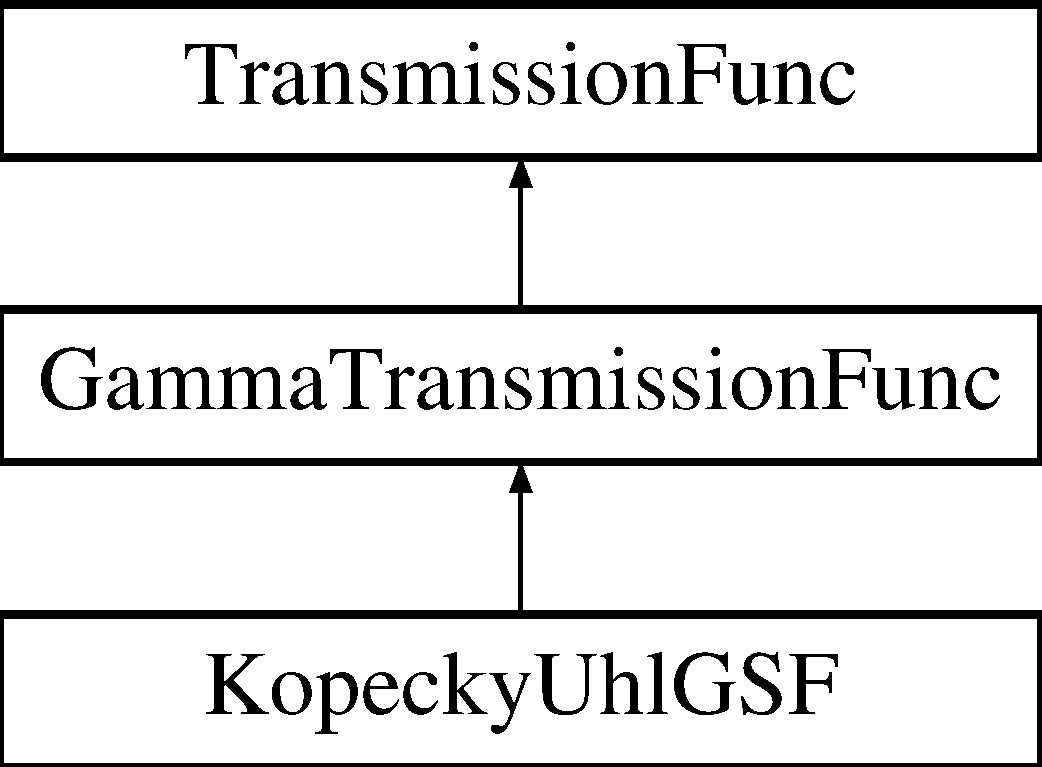
\includegraphics[height=3.000000cm]{d1/df2/classKopeckyUhlGSF}
\end{center}
\end{figure}
\subsection*{Public Member Functions}
\begin{DoxyCompactItemize}
\item 
\hyperlink{classKopeckyUhlGSF_a6d18795b6306d3bd01c9d7b097de2f3c}{Kopecky\-Uhl\-G\-S\-F} (int, int, double, int, double, int, double, double, double, double, \hyperlink{classTransmissionFunc}{Transmission\-Func} $\ast$, \hyperlink{classLevelDensity}{Level\-Density} $\ast$, double)
\item 
double \hyperlink{classKopeckyUhlGSF_acc719c087bb05ab9cc679c07d887b3ad}{Calc\-Strength\-Function} (double)
\end{DoxyCompactItemize}
\subsection*{Additional Inherited Members}


\subsection{Constructor \& Destructor Documentation}
\hypertarget{classKopeckyUhlGSF_a6d18795b6306d3bd01c9d7b097de2f3c}{\index{Kopecky\-Uhl\-G\-S\-F@{Kopecky\-Uhl\-G\-S\-F}!Kopecky\-Uhl\-G\-S\-F@{Kopecky\-Uhl\-G\-S\-F}}
\index{Kopecky\-Uhl\-G\-S\-F@{Kopecky\-Uhl\-G\-S\-F}!KopeckyUhlGSF@{Kopecky\-Uhl\-G\-S\-F}}
\subsubsection[{Kopecky\-Uhl\-G\-S\-F}]{\setlength{\rightskip}{0pt plus 5cm}Kopecky\-Uhl\-G\-S\-F\-::\-Kopecky\-Uhl\-G\-S\-F (
\begin{DoxyParamCaption}
\item[{int}]{z2, }
\item[{int}]{m2, }
\item[{double}]{j\-Initial, }
\item[{int}]{pi\-Initial, }
\item[{double}]{j\-Final, }
\item[{int}]{pi\-Final, }
\item[{double}]{max\-L, }
\item[{double}]{total\-Width\-For\-Correction, }
\item[{double}]{uncorr\-Total\-Width\-For\-Correction, }
\item[{double}]{uncorr\-Total\-Width\-Sqrd\-For\-Correction, }
\item[{{\bf Transmission\-Func} $\ast$}]{previous, }
\item[{{\bf Level\-Density} $\ast$}]{level\-Density, }
\item[{double}]{compound\-E}
\end{DoxyParamCaption}
)}}\label{classKopeckyUhlGSF_a6d18795b6306d3bd01c9d7b097de2f3c}


References Level\-Density\-::backshift\-\_\-, Level\-Density\-::\-Calc\-Density\-Param(), and Nuclear\-Mass\-::\-Q\-Value().



\subsection{Member Function Documentation}
\hypertarget{classKopeckyUhlGSF_acc719c087bb05ab9cc679c07d887b3ad}{\index{Kopecky\-Uhl\-G\-S\-F@{Kopecky\-Uhl\-G\-S\-F}!Calc\-Strength\-Function@{Calc\-Strength\-Function}}
\index{Calc\-Strength\-Function@{Calc\-Strength\-Function}!KopeckyUhlGSF@{Kopecky\-Uhl\-G\-S\-F}}
\subsubsection[{Calc\-Strength\-Function}]{\setlength{\rightskip}{0pt plus 5cm}double Kopecky\-Uhl\-G\-S\-F\-::\-Calc\-Strength\-Function (
\begin{DoxyParamCaption}
\item[{double}]{energy}
\end{DoxyParamCaption}
)\hspace{0.3cm}{\ttfamily [virtual]}}}\label{classKopeckyUhlGSF_acc719c087bb05ab9cc679c07d887b3ad}


Implements \hyperlink{classGammaTransmissionFunc_a68156d72ed9620f66f96dc37bbf781aa}{Gamma\-Transmission\-Func}.



References G\-D\-R\-Parameters\-::\-E\-\_\-, Gamma\-Transmission\-Func\-::gdr\-Parameters\-\_\-, G\-D\-R\-Parameters\-::k\-Sigma\-Gamma\-\_\-, pi, and G\-D\-R\-Parameters\-::\-W\-\_\-.



The documentation for this class was generated from the following files\-:\begin{DoxyCompactItemize}
\item 
/afs/crc.\-nd.\-edu/user/p/pscholz/\-Private/sapphire-\/devel/include/\hyperlink{KopeckyUhlGSF_8h}{Kopecky\-Uhl\-G\-S\-F.\-h}\item 
/afs/crc.\-nd.\-edu/user/p/pscholz/\-Private/sapphire-\/devel/src/\hyperlink{KopeckyUhlGSF_8cpp}{Kopecky\-Uhl\-G\-S\-F.\-cpp}\end{DoxyCompactItemize}

\hypertarget{classLevel}{\section{Level Class Reference}
\label{classLevel}\index{Level@{Level}}
}


{\ttfamily \#include $<$Nuclear\-Levels.\-h$>$}

\subsection*{Public Member Functions}
\begin{DoxyCompactItemize}
\item 
\hyperlink{classLevel_ac2fca00ede2f86939e5c71015e936566}{Level} (double J, int Pi, double energy)
\end{DoxyCompactItemize}
\subsection*{Public Attributes}
\begin{DoxyCompactItemize}
\item 
int \hyperlink{classLevel_a3cee365520b4879a70dfb4362fe59fe3}{Pi\-\_\-}
\item 
double \hyperlink{classLevel_aa0a9158f0edaed1fedd27f310db4d344}{J\-\_\-}
\item 
double \hyperlink{classLevel_ad7a1c3e9c9af88945e4d80016251cdaf}{energy\-\_\-}
\item 
std\-::vector$<$ \hyperlink{classGammaTransition}{Gamma\-Transition} $>$ \hyperlink{classLevel_a11037583b37641411f0811740053ed33}{gammas\-\_\-}
\end{DoxyCompactItemize}


\subsection{Constructor \& Destructor Documentation}
\hypertarget{classLevel_ac2fca00ede2f86939e5c71015e936566}{\index{Level@{Level}!Level@{Level}}
\index{Level@{Level}!Level@{Level}}
\subsubsection[{Level}]{\setlength{\rightskip}{0pt plus 5cm}Level\-::\-Level (
\begin{DoxyParamCaption}
\item[{double}]{J, }
\item[{int}]{Pi, }
\item[{double}]{energy}
\end{DoxyParamCaption}
)\hspace{0.3cm}{\ttfamily [inline]}}}\label{classLevel_ac2fca00ede2f86939e5c71015e936566}


\subsection{Member Data Documentation}
\hypertarget{classLevel_ad7a1c3e9c9af88945e4d80016251cdaf}{\index{Level@{Level}!energy\-\_\-@{energy\-\_\-}}
\index{energy\-\_\-@{energy\-\_\-}!Level@{Level}}
\subsubsection[{energy\-\_\-}]{\setlength{\rightskip}{0pt plus 5cm}double Level\-::energy\-\_\-}}\label{classLevel_ad7a1c3e9c9af88945e4d80016251cdaf}


Referenced by Cross\-Section\-::\-Cross\-Section().

\hypertarget{classLevel_a11037583b37641411f0811740053ed33}{\index{Level@{Level}!gammas\-\_\-@{gammas\-\_\-}}
\index{gammas\-\_\-@{gammas\-\_\-}!Level@{Level}}
\subsubsection[{gammas\-\_\-}]{\setlength{\rightskip}{0pt plus 5cm}std\-::vector$<${\bf Gamma\-Transition}$>$ Level\-::gammas\-\_\-}}\label{classLevel_a11037583b37641411f0811740053ed33}


Referenced by Levels\-Container\-::\-Levels\-Container().

\hypertarget{classLevel_aa0a9158f0edaed1fedd27f310db4d344}{\index{Level@{Level}!J\-\_\-@{J\-\_\-}}
\index{J\-\_\-@{J\-\_\-}!Level@{Level}}
\subsubsection[{J\-\_\-}]{\setlength{\rightskip}{0pt plus 5cm}double Level\-::\-J\-\_\-}}\label{classLevel_aa0a9158f0edaed1fedd27f310db4d344}


Referenced by Cross\-Section\-::\-Cross\-Section().

\hypertarget{classLevel_a3cee365520b4879a70dfb4362fe59fe3}{\index{Level@{Level}!Pi\-\_\-@{Pi\-\_\-}}
\index{Pi\-\_\-@{Pi\-\_\-}!Level@{Level}}
\subsubsection[{Pi\-\_\-}]{\setlength{\rightskip}{0pt plus 5cm}int Level\-::\-Pi\-\_\-}}\label{classLevel_a3cee365520b4879a70dfb4362fe59fe3}


Referenced by Cross\-Section\-::\-Cross\-Section().



The documentation for this class was generated from the following file\-:\begin{DoxyCompactItemize}
\item 
/afs/crc.\-nd.\-edu/user/p/pscholz/\-Private/sapphire-\/devel/include/\hyperlink{NuclearLevels_8h}{Nuclear\-Levels.\-h}\end{DoxyCompactItemize}

\hypertarget{classLevelDensity}{\section{Level\-Density Class Reference}
\label{classLevelDensity}\index{Level\-Density@{Level\-Density}}
}


{\ttfamily \#include $<$Level\-Density.\-h$>$}

Inheritance diagram for Level\-Density\-:\begin{figure}[H]
\begin{center}
\leavevmode
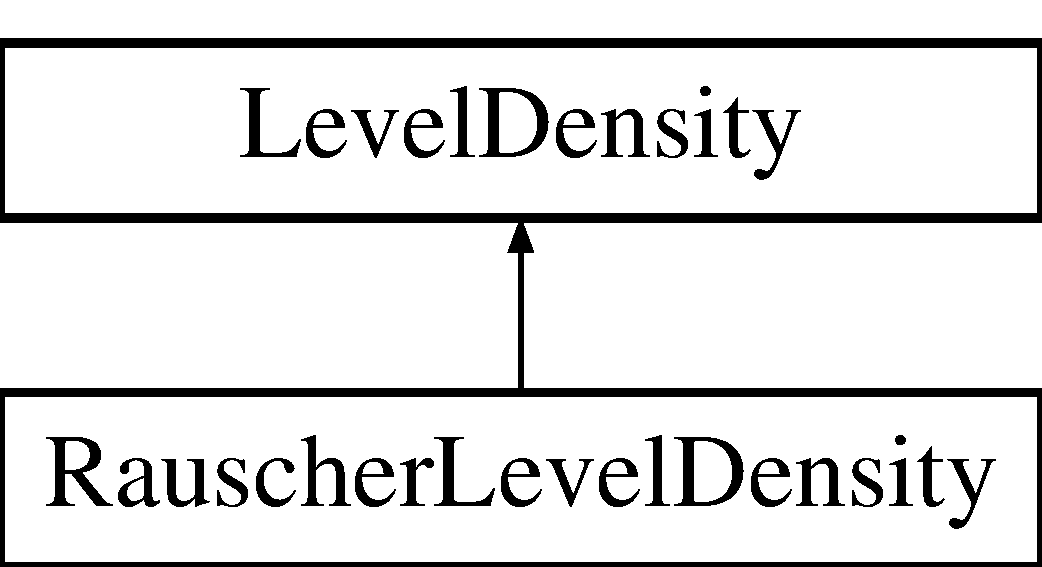
\includegraphics[height=2.000000cm]{d5/d00/classLevelDensity}
\end{center}
\end{figure}
\subsection*{Public Member Functions}
\begin{DoxyCompactItemize}
\item 
\hyperlink{classLevelDensity_ae38bbf8823d4edf4d78ae36cfb06c49f}{Level\-Density} (int Z, int A, double J)
\item 
virtual \hyperlink{classLevelDensity_abe9cc580b71e8c0adfb4f137778cd17b}{$\sim$\-Level\-Density} ()
\item 
double \hyperlink{classLevelDensity_a7ac3ac01c14a34c727cb60c485a5653d}{operator()} (double)
\item 
double \hyperlink{classLevelDensity_aaf525f64721eaf5cc8e32b1147818864}{Total\-Level\-Density} (double)
\end{DoxyCompactItemize}
\subsection*{Protected Member Functions}
\begin{DoxyCompactItemize}
\item 
virtual void \hyperlink{classLevelDensity_a2aa1bbc8192a97c45be4f049dbd2dcc0}{Calc\-Back\-Shift} ()=0
\item 
virtual double \hyperlink{classLevelDensity_a42de1e15ee79bc984923b29b44ec55d5}{Calc\-Density\-Param} (double)=0
\item 
virtual double \hyperlink{classLevelDensity_a6a19c56e9784c0f1dac0ca2b86397c20}{Calc\-Nuclear\-Temp} (double)=0
\item 
void \hyperlink{classLevelDensity_ab113ee9e46b56bd88e02da587389e885}{Calc\-Constant\-Temp\-Terms} ()
\end{DoxyCompactItemize}
\subsection*{Protected Attributes}
\begin{DoxyCompactItemize}
\item 
int \hyperlink{classLevelDensity_a4e3c2f3637a11130dc5d0504bf0af9c9}{Z\-\_\-}
\item 
int \hyperlink{classLevelDensity_a49a372560d87e4bfda8759eb315a10ed}{A\-\_\-}
\item 
double \hyperlink{classLevelDensity_a20733f689cc018869ef19f2e6bcd3c87}{J\-\_\-}
\item 
double \hyperlink{classLevelDensity_ab38ac8b223b47b3f627b1d1443168b28}{backshift\-\_\-}
\item 
double \hyperlink{classLevelDensity_a580dc958baa563bf774a0a6f6b4fea7e}{critical\-U\-\_\-}
\item 
double \hyperlink{classLevelDensity_acfc91464640c910baac56f85751b7dac}{const\-Ang\-Term\-\_\-}
\item 
double \hyperlink{classLevelDensity_a7a97d015ef2f00caa58af1854ee492ca}{nuclear\-Temp\-\_\-}
\item 
double \hyperlink{classLevelDensity_a61c66e8f640cbffe7d2977d69981e30c}{e0\-\_\-}
\end{DoxyCompactItemize}
\subsection*{Static Protected Attributes}
\begin{DoxyCompactItemize}
\item 
static const double \hyperlink{classLevelDensity_a0b95afe91b297932f43c75cbcedf3ff9}{zeta\-\_\-} = 1.\-0
\item 
static const double \hyperlink{classLevelDensity_afbfc27a16a0ef3a990dce6ef5acf7863}{r0\-\_\-} = 1.\-25
\end{DoxyCompactItemize}
\subsection*{Friends}
\begin{DoxyCompactItemize}
\item 
class \hyperlink{classLevelDensity_a82f9f4a3eb74ca7e08cb54054e30cd76}{Kopecky\-Uhl\-G\-S\-F}
\end{DoxyCompactItemize}


\subsection{Constructor \& Destructor Documentation}
\hypertarget{classLevelDensity_ae38bbf8823d4edf4d78ae36cfb06c49f}{\index{Level\-Density@{Level\-Density}!Level\-Density@{Level\-Density}}
\index{Level\-Density@{Level\-Density}!LevelDensity@{Level\-Density}}
\subsubsection[{Level\-Density}]{\setlength{\rightskip}{0pt plus 5cm}Level\-Density\-::\-Level\-Density (
\begin{DoxyParamCaption}
\item[{int}]{Z, }
\item[{int}]{A, }
\item[{double}]{J}
\end{DoxyParamCaption}
)\hspace{0.3cm}{\ttfamily [inline]}}}\label{classLevelDensity_ae38bbf8823d4edf4d78ae36cfb06c49f}


References critical\-U\-\_\-.

\hypertarget{classLevelDensity_abe9cc580b71e8c0adfb4f137778cd17b}{\index{Level\-Density@{Level\-Density}!$\sim$\-Level\-Density@{$\sim$\-Level\-Density}}
\index{$\sim$\-Level\-Density@{$\sim$\-Level\-Density}!LevelDensity@{Level\-Density}}
\subsubsection[{$\sim$\-Level\-Density}]{\setlength{\rightskip}{0pt plus 5cm}virtual Level\-Density\-::$\sim$\-Level\-Density (
\begin{DoxyParamCaption}
{}
\end{DoxyParamCaption}
)\hspace{0.3cm}{\ttfamily [inline]}, {\ttfamily [virtual]}}}\label{classLevelDensity_abe9cc580b71e8c0adfb4f137778cd17b}


\subsection{Member Function Documentation}
\hypertarget{classLevelDensity_a2aa1bbc8192a97c45be4f049dbd2dcc0}{\index{Level\-Density@{Level\-Density}!Calc\-Back\-Shift@{Calc\-Back\-Shift}}
\index{Calc\-Back\-Shift@{Calc\-Back\-Shift}!LevelDensity@{Level\-Density}}
\subsubsection[{Calc\-Back\-Shift}]{\setlength{\rightskip}{0pt plus 5cm}virtual void Level\-Density\-::\-Calc\-Back\-Shift (
\begin{DoxyParamCaption}
{}
\end{DoxyParamCaption}
)\hspace{0.3cm}{\ttfamily [protected]}, {\ttfamily [pure virtual]}}}\label{classLevelDensity_a2aa1bbc8192a97c45be4f049dbd2dcc0}


Implemented in \hyperlink{classRauscherLevelDensity_af5ce4f61ab69164ea0e8e47a4ed688c4}{Rauscher\-Level\-Density}.

\hypertarget{classLevelDensity_ab113ee9e46b56bd88e02da587389e885}{\index{Level\-Density@{Level\-Density}!Calc\-Constant\-Temp\-Terms@{Calc\-Constant\-Temp\-Terms}}
\index{Calc\-Constant\-Temp\-Terms@{Calc\-Constant\-Temp\-Terms}!LevelDensity@{Level\-Density}}
\subsubsection[{Calc\-Constant\-Temp\-Terms}]{\setlength{\rightskip}{0pt plus 5cm}void Level\-Density\-::\-Calc\-Constant\-Temp\-Terms (
\begin{DoxyParamCaption}
{}
\end{DoxyParamCaption}
)\hspace{0.3cm}{\ttfamily [protected]}}}\label{classLevelDensity_ab113ee9e46b56bd88e02da587389e885}


References A\-\_\-, backshift\-\_\-, Calc\-Density\-Param(), Calc\-Nuclear\-Temp(), const\-Ang\-Term\-\_\-, critical\-U\-\_\-, e0\-\_\-, hbarc, J\-\_\-, nuclear\-Temp\-\_\-, r0\-\_\-, uconv, and zeta\-\_\-.



Referenced by Rauscher\-Level\-Density\-::\-Rauscher\-Level\-Density().

\hypertarget{classLevelDensity_a42de1e15ee79bc984923b29b44ec55d5}{\index{Level\-Density@{Level\-Density}!Calc\-Density\-Param@{Calc\-Density\-Param}}
\index{Calc\-Density\-Param@{Calc\-Density\-Param}!LevelDensity@{Level\-Density}}
\subsubsection[{Calc\-Density\-Param}]{\setlength{\rightskip}{0pt plus 5cm}virtual double Level\-Density\-::\-Calc\-Density\-Param (
\begin{DoxyParamCaption}
\item[{double}]{}
\end{DoxyParamCaption}
)\hspace{0.3cm}{\ttfamily [protected]}, {\ttfamily [pure virtual]}}}\label{classLevelDensity_a42de1e15ee79bc984923b29b44ec55d5}


Implemented in \hyperlink{classRauscherLevelDensity_a842444681f72b30d3dfbdf18ba95b207}{Rauscher\-Level\-Density}.



Referenced by Calc\-Constant\-Temp\-Terms(), Kopecky\-Uhl\-G\-S\-F\-::\-Kopecky\-Uhl\-G\-S\-F(), operator()(), and Total\-Level\-Density().

\hypertarget{classLevelDensity_a6a19c56e9784c0f1dac0ca2b86397c20}{\index{Level\-Density@{Level\-Density}!Calc\-Nuclear\-Temp@{Calc\-Nuclear\-Temp}}
\index{Calc\-Nuclear\-Temp@{Calc\-Nuclear\-Temp}!LevelDensity@{Level\-Density}}
\subsubsection[{Calc\-Nuclear\-Temp}]{\setlength{\rightskip}{0pt plus 5cm}virtual double Level\-Density\-::\-Calc\-Nuclear\-Temp (
\begin{DoxyParamCaption}
\item[{double}]{}
\end{DoxyParamCaption}
)\hspace{0.3cm}{\ttfamily [protected]}, {\ttfamily [pure virtual]}}}\label{classLevelDensity_a6a19c56e9784c0f1dac0ca2b86397c20}


Implemented in \hyperlink{classRauscherLevelDensity_a734ed056ae869367c1cf295503c9d6aa}{Rauscher\-Level\-Density}.



Referenced by Calc\-Constant\-Temp\-Terms().

\hypertarget{classLevelDensity_a7ac3ac01c14a34c727cb60c485a5653d}{\index{Level\-Density@{Level\-Density}!operator()@{operator()}}
\index{operator()@{operator()}!LevelDensity@{Level\-Density}}
\subsubsection[{operator()}]{\setlength{\rightskip}{0pt plus 5cm}double Level\-Density\-::operator() (
\begin{DoxyParamCaption}
\item[{double}]{E}
\end{DoxyParamCaption}
)}}\label{classLevelDensity_a7ac3ac01c14a34c727cb60c485a5653d}


References A\-\_\-, backshift\-\_\-, Calc\-Density\-Param(), const\-Ang\-Term\-\_\-, critical\-U\-\_\-, gsl\-\_\-partfunc\-\_\-params\-::density, e0\-\_\-, hbarc, J\-\_\-, nuclear\-Temp\-\_\-, r0\-\_\-, uconv, and zeta\-\_\-.

\hypertarget{classLevelDensity_aaf525f64721eaf5cc8e32b1147818864}{\index{Level\-Density@{Level\-Density}!Total\-Level\-Density@{Total\-Level\-Density}}
\index{Total\-Level\-Density@{Total\-Level\-Density}!LevelDensity@{Level\-Density}}
\subsubsection[{Total\-Level\-Density}]{\setlength{\rightskip}{0pt plus 5cm}double Level\-Density\-::\-Total\-Level\-Density (
\begin{DoxyParamCaption}
\item[{double}]{E}
\end{DoxyParamCaption}
)}}\label{classLevelDensity_aaf525f64721eaf5cc8e32b1147818864}


References A\-\_\-, backshift\-\_\-, Calc\-Density\-Param(), critical\-U\-\_\-, gsl\-\_\-partfunc\-\_\-params\-::density, e0\-\_\-, hbarc, nuclear\-Temp\-\_\-, r0\-\_\-, uconv, and zeta\-\_\-.



Referenced by Transition\-Rate\-Func\-::\-Calc\-Total\-Level\-Density().



\subsection{Friends And Related Function Documentation}
\hypertarget{classLevelDensity_a82f9f4a3eb74ca7e08cb54054e30cd76}{\index{Level\-Density@{Level\-Density}!Kopecky\-Uhl\-G\-S\-F@{Kopecky\-Uhl\-G\-S\-F}}
\index{Kopecky\-Uhl\-G\-S\-F@{Kopecky\-Uhl\-G\-S\-F}!LevelDensity@{Level\-Density}}
\subsubsection[{Kopecky\-Uhl\-G\-S\-F}]{\setlength{\rightskip}{0pt plus 5cm}friend class {\bf Kopecky\-Uhl\-G\-S\-F}\hspace{0.3cm}{\ttfamily [friend]}}}\label{classLevelDensity_a82f9f4a3eb74ca7e08cb54054e30cd76}


\subsection{Member Data Documentation}
\hypertarget{classLevelDensity_a49a372560d87e4bfda8759eb315a10ed}{\index{Level\-Density@{Level\-Density}!A\-\_\-@{A\-\_\-}}
\index{A\-\_\-@{A\-\_\-}!LevelDensity@{Level\-Density}}
\subsubsection[{A\-\_\-}]{\setlength{\rightskip}{0pt plus 5cm}int Level\-Density\-::\-A\-\_\-\hspace{0.3cm}{\ttfamily [protected]}}}\label{classLevelDensity_a49a372560d87e4bfda8759eb315a10ed}


Referenced by Rauscher\-Level\-Density\-::\-Calc\-Back\-Shift(), Calc\-Constant\-Temp\-Terms(), operator()(), and Total\-Level\-Density().

\hypertarget{classLevelDensity_ab38ac8b223b47b3f627b1d1443168b28}{\index{Level\-Density@{Level\-Density}!backshift\-\_\-@{backshift\-\_\-}}
\index{backshift\-\_\-@{backshift\-\_\-}!LevelDensity@{Level\-Density}}
\subsubsection[{backshift\-\_\-}]{\setlength{\rightskip}{0pt plus 5cm}double Level\-Density\-::backshift\-\_\-\hspace{0.3cm}{\ttfamily [protected]}}}\label{classLevelDensity_ab38ac8b223b47b3f627b1d1443168b28}


Referenced by Rauscher\-Level\-Density\-::\-Calc\-Back\-Shift(), Calc\-Constant\-Temp\-Terms(), Kopecky\-Uhl\-G\-S\-F\-::\-Kopecky\-Uhl\-G\-S\-F(), operator()(), and Total\-Level\-Density().

\hypertarget{classLevelDensity_acfc91464640c910baac56f85751b7dac}{\index{Level\-Density@{Level\-Density}!const\-Ang\-Term\-\_\-@{const\-Ang\-Term\-\_\-}}
\index{const\-Ang\-Term\-\_\-@{const\-Ang\-Term\-\_\-}!LevelDensity@{Level\-Density}}
\subsubsection[{const\-Ang\-Term\-\_\-}]{\setlength{\rightskip}{0pt plus 5cm}double Level\-Density\-::const\-Ang\-Term\-\_\-\hspace{0.3cm}{\ttfamily [protected]}}}\label{classLevelDensity_acfc91464640c910baac56f85751b7dac}


Referenced by Calc\-Constant\-Temp\-Terms(), and operator()().

\hypertarget{classLevelDensity_a580dc958baa563bf774a0a6f6b4fea7e}{\index{Level\-Density@{Level\-Density}!critical\-U\-\_\-@{critical\-U\-\_\-}}
\index{critical\-U\-\_\-@{critical\-U\-\_\-}!LevelDensity@{Level\-Density}}
\subsubsection[{critical\-U\-\_\-}]{\setlength{\rightskip}{0pt plus 5cm}double Level\-Density\-::critical\-U\-\_\-\hspace{0.3cm}{\ttfamily [protected]}}}\label{classLevelDensity_a580dc958baa563bf774a0a6f6b4fea7e}


Referenced by Calc\-Constant\-Temp\-Terms(), Level\-Density(), operator()(), and Total\-Level\-Density().

\hypertarget{classLevelDensity_a61c66e8f640cbffe7d2977d69981e30c}{\index{Level\-Density@{Level\-Density}!e0\-\_\-@{e0\-\_\-}}
\index{e0\-\_\-@{e0\-\_\-}!LevelDensity@{Level\-Density}}
\subsubsection[{e0\-\_\-}]{\setlength{\rightskip}{0pt plus 5cm}double Level\-Density\-::e0\-\_\-\hspace{0.3cm}{\ttfamily [protected]}}}\label{classLevelDensity_a61c66e8f640cbffe7d2977d69981e30c}


Referenced by Calc\-Constant\-Temp\-Terms(), operator()(), and Total\-Level\-Density().

\hypertarget{classLevelDensity_a20733f689cc018869ef19f2e6bcd3c87}{\index{Level\-Density@{Level\-Density}!J\-\_\-@{J\-\_\-}}
\index{J\-\_\-@{J\-\_\-}!LevelDensity@{Level\-Density}}
\subsubsection[{J\-\_\-}]{\setlength{\rightskip}{0pt plus 5cm}double Level\-Density\-::\-J\-\_\-\hspace{0.3cm}{\ttfamily [protected]}}}\label{classLevelDensity_a20733f689cc018869ef19f2e6bcd3c87}


Referenced by Calc\-Constant\-Temp\-Terms(), and operator()().

\hypertarget{classLevelDensity_a7a97d015ef2f00caa58af1854ee492ca}{\index{Level\-Density@{Level\-Density}!nuclear\-Temp\-\_\-@{nuclear\-Temp\-\_\-}}
\index{nuclear\-Temp\-\_\-@{nuclear\-Temp\-\_\-}!LevelDensity@{Level\-Density}}
\subsubsection[{nuclear\-Temp\-\_\-}]{\setlength{\rightskip}{0pt plus 5cm}double Level\-Density\-::nuclear\-Temp\-\_\-\hspace{0.3cm}{\ttfamily [protected]}}}\label{classLevelDensity_a7a97d015ef2f00caa58af1854ee492ca}


Referenced by Calc\-Constant\-Temp\-Terms(), operator()(), and Total\-Level\-Density().

\hypertarget{classLevelDensity_afbfc27a16a0ef3a990dce6ef5acf7863}{\index{Level\-Density@{Level\-Density}!r0\-\_\-@{r0\-\_\-}}
\index{r0\-\_\-@{r0\-\_\-}!LevelDensity@{Level\-Density}}
\subsubsection[{r0\-\_\-}]{\setlength{\rightskip}{0pt plus 5cm}const double Level\-Density\-::r0\-\_\- = 1.\-25\hspace{0.3cm}{\ttfamily [static]}, {\ttfamily [protected]}}}\label{classLevelDensity_afbfc27a16a0ef3a990dce6ef5acf7863}


Referenced by Calc\-Constant\-Temp\-Terms(), operator()(), and Total\-Level\-Density().

\hypertarget{classLevelDensity_a4e3c2f3637a11130dc5d0504bf0af9c9}{\index{Level\-Density@{Level\-Density}!Z\-\_\-@{Z\-\_\-}}
\index{Z\-\_\-@{Z\-\_\-}!LevelDensity@{Level\-Density}}
\subsubsection[{Z\-\_\-}]{\setlength{\rightskip}{0pt plus 5cm}int Level\-Density\-::\-Z\-\_\-\hspace{0.3cm}{\ttfamily [protected]}}}\label{classLevelDensity_a4e3c2f3637a11130dc5d0504bf0af9c9}


Referenced by Rauscher\-Level\-Density\-::\-Calc\-Back\-Shift().

\hypertarget{classLevelDensity_a0b95afe91b297932f43c75cbcedf3ff9}{\index{Level\-Density@{Level\-Density}!zeta\-\_\-@{zeta\-\_\-}}
\index{zeta\-\_\-@{zeta\-\_\-}!LevelDensity@{Level\-Density}}
\subsubsection[{zeta\-\_\-}]{\setlength{\rightskip}{0pt plus 5cm}const double Level\-Density\-::zeta\-\_\- = 1.\-0\hspace{0.3cm}{\ttfamily [static]}, {\ttfamily [protected]}}}\label{classLevelDensity_a0b95afe91b297932f43c75cbcedf3ff9}


Referenced by Calc\-Constant\-Temp\-Terms(), operator()(), and Total\-Level\-Density().



The documentation for this class was generated from the following files\-:\begin{DoxyCompactItemize}
\item 
include/\hyperlink{LevelDensity_8h}{Level\-Density.\-h}\item 
src/\hyperlink{LevelDensity_8cpp}{Level\-Density.\-cpp}\end{DoxyCompactItemize}

\hypertarget{classLevelsContainer}{\section{Levels\-Container Class Reference}
\label{classLevelsContainer}\index{Levels\-Container@{Levels\-Container}}
}


{\ttfamily \#include $<$Nuclear\-Levels.\-h$>$}

\subsection*{Public Member Functions}
\begin{DoxyCompactItemize}
\item 
\hyperlink{classLevelsContainer_a58e643cd8ba5a8a9b3c9c02d5b427781}{Levels\-Container} ()
\item 
\hyperlink{classLevelsContainer_a398a15211a87131c4418a8ab5b50e608}{Levels\-Container} (std\-::istream \&, int, int)
\end{DoxyCompactItemize}
\subsection*{Public Attributes}
\begin{DoxyCompactItemize}
\item 
std\-::vector$<$ \hyperlink{classLevel}{Level} $>$ \hyperlink{classLevelsContainer_a237727bb8b0c7f1a75701fde67d2094b}{levels\-\_\-}
\end{DoxyCompactItemize}


\subsection{Constructor \& Destructor Documentation}
\hypertarget{classLevelsContainer_a58e643cd8ba5a8a9b3c9c02d5b427781}{\index{Levels\-Container@{Levels\-Container}!Levels\-Container@{Levels\-Container}}
\index{Levels\-Container@{Levels\-Container}!LevelsContainer@{Levels\-Container}}
\subsubsection[{Levels\-Container}]{\setlength{\rightskip}{0pt plus 5cm}Levels\-Container\-::\-Levels\-Container (
\begin{DoxyParamCaption}
{}
\end{DoxyParamCaption}
)\hspace{0.3cm}{\ttfamily [inline]}}}\label{classLevelsContainer_a58e643cd8ba5a8a9b3c9c02d5b427781}
\hypertarget{classLevelsContainer_a398a15211a87131c4418a8ab5b50e608}{\index{Levels\-Container@{Levels\-Container}!Levels\-Container@{Levels\-Container}}
\index{Levels\-Container@{Levels\-Container}!LevelsContainer@{Levels\-Container}}
\subsubsection[{Levels\-Container}]{\setlength{\rightskip}{0pt plus 5cm}Levels\-Container\-::\-Levels\-Container (
\begin{DoxyParamCaption}
\item[{std\-::istream \&}]{in, }
\item[{int}]{num\-Levels, }
\item[{int}]{num\-Complete}
\end{DoxyParamCaption}
)}}\label{classLevelsContainer_a398a15211a87131c4418a8ab5b50e608}


References Level\-::gammas\-\_\-, and levels\-\_\-.



\subsection{Member Data Documentation}
\hypertarget{classLevelsContainer_a237727bb8b0c7f1a75701fde67d2094b}{\index{Levels\-Container@{Levels\-Container}!levels\-\_\-@{levels\-\_\-}}
\index{levels\-\_\-@{levels\-\_\-}!LevelsContainer@{Levels\-Container}}
\subsubsection[{levels\-\_\-}]{\setlength{\rightskip}{0pt plus 5cm}std\-::vector$<${\bf Level}$>$ Levels\-Container\-::levels\-\_\-}}\label{classLevelsContainer_a237727bb8b0c7f1a75701fde67d2094b}


Referenced by Nuclear\-Levels\-::\-Initialize\-Levels(), and Levels\-Container().



The documentation for this class was generated from the following files\-:\begin{DoxyCompactItemize}
\item 
include/\hyperlink{NuclearLevels_8h}{Nuclear\-Levels.\-h}\item 
src/\hyperlink{NuclearLevels_8cpp}{Nuclear\-Levels.\-cpp}\end{DoxyCompactItemize}

\hypertarget{classMassEntry}{\section{Mass\-Entry Class Reference}
\label{classMassEntry}\index{Mass\-Entry@{Mass\-Entry}}
}


{\ttfamily \#include $<$Nuclear\-Mass.\-h$>$}

\subsection*{Public Member Functions}
\begin{DoxyCompactItemize}
\item 
\hyperlink{classMassEntry_aba724f4d33386d8ac391e234d19961a1}{Mass\-Entry} ()
\item 
\hyperlink{classMassEntry_a845d274a437da70ce7e9d09d9a93551b}{Mass\-Entry} (double exp\-Mass, double th\-Mass, double micro\-Energy\-Corr, unsigned int mask)
\end{DoxyCompactItemize}
\subsection*{Public Attributes}
\begin{DoxyCompactItemize}
\item 
double \hyperlink{classMassEntry_a29ee91e9e1063f99766a56b827cf0f8c}{exp\-Mass\-\_\-}
\item 
double \hyperlink{classMassEntry_a8fd951ec49bba7068699a48c44e9041b}{th\-Mass\-\_\-}
\item 
double \hyperlink{classMassEntry_a27bea79c386c9d242d73c6e99f2d69c9}{micro\-Energy\-Corr\-\_\-}
\item 
unsigned int \hyperlink{classMassEntry_a22d01d36521f35952e3b605a4f201ffb}{mask\-\_\-}
\end{DoxyCompactItemize}


\subsection{Constructor \& Destructor Documentation}
\hypertarget{classMassEntry_aba724f4d33386d8ac391e234d19961a1}{\index{Mass\-Entry@{Mass\-Entry}!Mass\-Entry@{Mass\-Entry}}
\index{Mass\-Entry@{Mass\-Entry}!MassEntry@{Mass\-Entry}}
\subsubsection[{Mass\-Entry}]{\setlength{\rightskip}{0pt plus 5cm}Mass\-Entry\-::\-Mass\-Entry (
\begin{DoxyParamCaption}
{}
\end{DoxyParamCaption}
)\hspace{0.3cm}{\ttfamily [inline]}}}\label{classMassEntry_aba724f4d33386d8ac391e234d19961a1}


References exp\-Mass\-\_\-, mask\-\_\-, micro\-Energy\-Corr\-\_\-, and th\-Mass\-\_\-.

\hypertarget{classMassEntry_a845d274a437da70ce7e9d09d9a93551b}{\index{Mass\-Entry@{Mass\-Entry}!Mass\-Entry@{Mass\-Entry}}
\index{Mass\-Entry@{Mass\-Entry}!MassEntry@{Mass\-Entry}}
\subsubsection[{Mass\-Entry}]{\setlength{\rightskip}{0pt plus 5cm}Mass\-Entry\-::\-Mass\-Entry (
\begin{DoxyParamCaption}
\item[{double}]{exp\-Mass, }
\item[{double}]{th\-Mass, }
\item[{double}]{micro\-Energy\-Corr, }
\item[{unsigned int}]{mask}
\end{DoxyParamCaption}
)\hspace{0.3cm}{\ttfamily [inline]}}}\label{classMassEntry_a845d274a437da70ce7e9d09d9a93551b}


\subsection{Member Data Documentation}
\hypertarget{classMassEntry_a29ee91e9e1063f99766a56b827cf0f8c}{\index{Mass\-Entry@{Mass\-Entry}!exp\-Mass\-\_\-@{exp\-Mass\-\_\-}}
\index{exp\-Mass\-\_\-@{exp\-Mass\-\_\-}!MassEntry@{Mass\-Entry}}
\subsubsection[{exp\-Mass\-\_\-}]{\setlength{\rightskip}{0pt plus 5cm}double Mass\-Entry\-::exp\-Mass\-\_\-}}\label{classMassEntry_a29ee91e9e1063f99766a56b827cf0f8c}


Referenced by Mass\-Entry().

\hypertarget{classMassEntry_a22d01d36521f35952e3b605a4f201ffb}{\index{Mass\-Entry@{Mass\-Entry}!mask\-\_\-@{mask\-\_\-}}
\index{mask\-\_\-@{mask\-\_\-}!MassEntry@{Mass\-Entry}}
\subsubsection[{mask\-\_\-}]{\setlength{\rightskip}{0pt plus 5cm}unsigned int Mass\-Entry\-::mask\-\_\-}}\label{classMassEntry_a22d01d36521f35952e3b605a4f201ffb}


Referenced by Mass\-Entry().

\hypertarget{classMassEntry_a27bea79c386c9d242d73c6e99f2d69c9}{\index{Mass\-Entry@{Mass\-Entry}!micro\-Energy\-Corr\-\_\-@{micro\-Energy\-Corr\-\_\-}}
\index{micro\-Energy\-Corr\-\_\-@{micro\-Energy\-Corr\-\_\-}!MassEntry@{Mass\-Entry}}
\subsubsection[{micro\-Energy\-Corr\-\_\-}]{\setlength{\rightskip}{0pt plus 5cm}double Mass\-Entry\-::micro\-Energy\-Corr\-\_\-}}\label{classMassEntry_a27bea79c386c9d242d73c6e99f2d69c9}


Referenced by Mass\-Entry().

\hypertarget{classMassEntry_a8fd951ec49bba7068699a48c44e9041b}{\index{Mass\-Entry@{Mass\-Entry}!th\-Mass\-\_\-@{th\-Mass\-\_\-}}
\index{th\-Mass\-\_\-@{th\-Mass\-\_\-}!MassEntry@{Mass\-Entry}}
\subsubsection[{th\-Mass\-\_\-}]{\setlength{\rightskip}{0pt plus 5cm}double Mass\-Entry\-::th\-Mass\-\_\-}}\label{classMassEntry_a8fd951ec49bba7068699a48c44e9041b}


Referenced by Mass\-Entry().



The documentation for this class was generated from the following file\-:\begin{DoxyCompactItemize}
\item 
/afs/crc.\-nd.\-edu/user/p/pscholz/\-Private/sapphire-\/devel/include/\hyperlink{NuclearMass_8h}{Nuclear\-Mass.\-h}\end{DoxyCompactItemize}

\hypertarget{classMassKey}{\section{Mass\-Key Class Reference}
\label{classMassKey}\index{Mass\-Key@{Mass\-Key}}
}


{\ttfamily \#include $<$Nuclear\-Mass.\-h$>$}

\subsection*{Public Member Functions}
\begin{DoxyCompactItemize}
\item 
\hyperlink{classMassKey_a11051c29b3f72af37f9ce2de9318d616}{Mass\-Key} (int Z, int A)
\item 
bool \hyperlink{classMassKey_a0c897aa37d045974bc7a54d4407ffc24}{operator$<$} (const \hyperlink{classMassKey}{Mass\-Key} \&right) const 
\end{DoxyCompactItemize}
\subsection*{Public Attributes}
\begin{DoxyCompactItemize}
\item 
int \hyperlink{classMassKey_a5f7b41c790d0a9aecb45a2a538e26684}{Z\-\_\-}
\item 
int \hyperlink{classMassKey_ae993028c1fda540cfb801b0900748a61}{A\-\_\-}
\end{DoxyCompactItemize}


\subsection{Constructor \& Destructor Documentation}
\hypertarget{classMassKey_a11051c29b3f72af37f9ce2de9318d616}{\index{Mass\-Key@{Mass\-Key}!Mass\-Key@{Mass\-Key}}
\index{Mass\-Key@{Mass\-Key}!MassKey@{Mass\-Key}}
\subsubsection[{Mass\-Key}]{\setlength{\rightskip}{0pt plus 5cm}Mass\-Key\-::\-Mass\-Key (
\begin{DoxyParamCaption}
\item[{int}]{Z, }
\item[{int}]{A}
\end{DoxyParamCaption}
)\hspace{0.3cm}{\ttfamily [inline]}}}\label{classMassKey_a11051c29b3f72af37f9ce2de9318d616}


\subsection{Member Function Documentation}
\hypertarget{classMassKey_a0c897aa37d045974bc7a54d4407ffc24}{\index{Mass\-Key@{Mass\-Key}!operator$<$@{operator$<$}}
\index{operator$<$@{operator$<$}!MassKey@{Mass\-Key}}
\subsubsection[{operator$<$}]{\setlength{\rightskip}{0pt plus 5cm}bool Mass\-Key\-::operator$<$ (
\begin{DoxyParamCaption}
\item[{const {\bf Mass\-Key} \&}]{right}
\end{DoxyParamCaption}
) const\hspace{0.3cm}{\ttfamily [inline]}}}\label{classMassKey_a0c897aa37d045974bc7a54d4407ffc24}


References A\-\_\-, and Z\-\_\-.



\subsection{Member Data Documentation}
\hypertarget{classMassKey_ae993028c1fda540cfb801b0900748a61}{\index{Mass\-Key@{Mass\-Key}!A\-\_\-@{A\-\_\-}}
\index{A\-\_\-@{A\-\_\-}!MassKey@{Mass\-Key}}
\subsubsection[{A\-\_\-}]{\setlength{\rightskip}{0pt plus 5cm}int Mass\-Key\-::\-A\-\_\-}}\label{classMassKey_ae993028c1fda540cfb801b0900748a61}


Referenced by std\-::tr1\-::hash$<$ Mass\-Key $>$\-::operator()(), std\-::equal\-\_\-to$<$ Mass\-Key $>$\-::operator()(), and operator$<$().

\hypertarget{classMassKey_a5f7b41c790d0a9aecb45a2a538e26684}{\index{Mass\-Key@{Mass\-Key}!Z\-\_\-@{Z\-\_\-}}
\index{Z\-\_\-@{Z\-\_\-}!MassKey@{Mass\-Key}}
\subsubsection[{Z\-\_\-}]{\setlength{\rightskip}{0pt plus 5cm}int Mass\-Key\-::\-Z\-\_\-}}\label{classMassKey_a5f7b41c790d0a9aecb45a2a538e26684}


Referenced by std\-::tr1\-::hash$<$ Mass\-Key $>$\-::operator()(), std\-::equal\-\_\-to$<$ Mass\-Key $>$\-::operator()(), and operator$<$().



The documentation for this class was generated from the following file\-:\begin{DoxyCompactItemize}
\item 
/afs/crc.\-nd.\-edu/user/p/pscholz/\-Private/sapphire-\/devel/include/\hyperlink{NuclearMass_8h}{Nuclear\-Mass.\-h}\end{DoxyCompactItemize}

\hypertarget{classMcCullaghGSF}{\section{Mc\-Cullagh\-G\-S\-F Class Reference}
\label{classMcCullaghGSF}\index{Mc\-Cullagh\-G\-S\-F@{Mc\-Cullagh\-G\-S\-F}}
}


{\ttfamily \#include $<$Mc\-Cullagh\-G\-S\-F.\-h$>$}

Inheritance diagram for Mc\-Cullagh\-G\-S\-F\-:\begin{figure}[H]
\begin{center}
\leavevmode
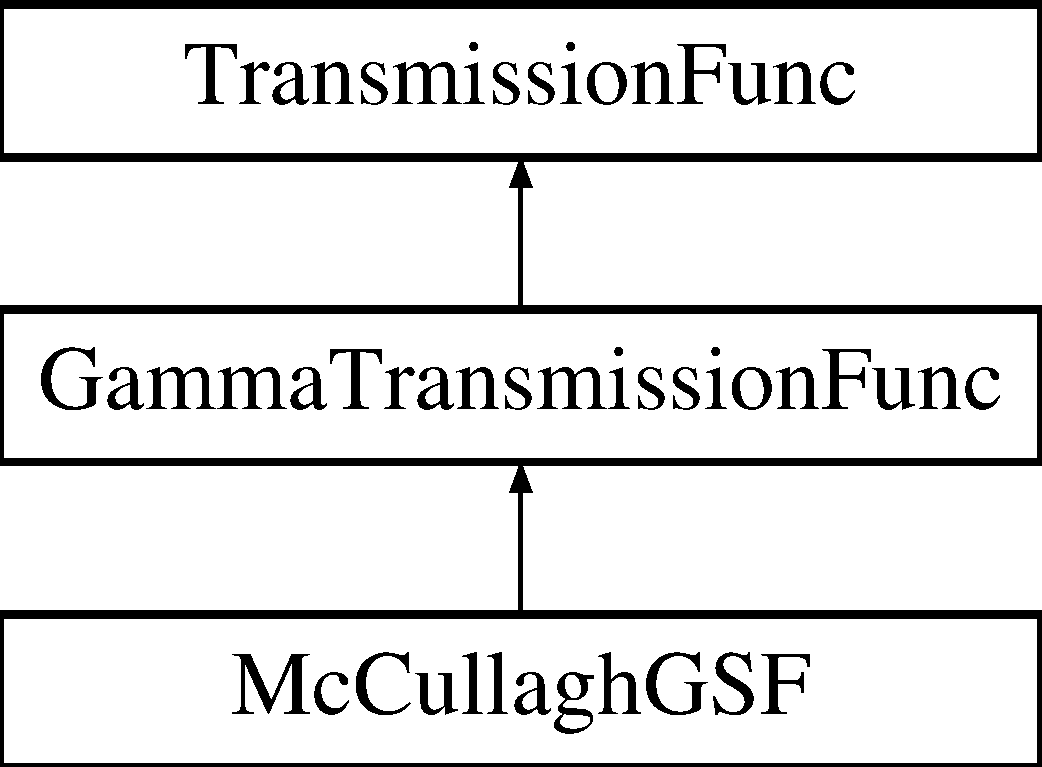
\includegraphics[height=3.000000cm]{da/d68/classMcCullaghGSF}
\end{center}
\end{figure}
\subsection*{Public Member Functions}
\begin{DoxyCompactItemize}
\item 
\hyperlink{classMcCullaghGSF_a4bdf71c12c6728bbeb4eff21fb7d0217}{Mc\-Cullagh\-G\-S\-F} (int, int, double, int, double, int, double, double, double, double, \hyperlink{classTransmissionFunc}{Transmission\-Func} $\ast$)
\item 
double \hyperlink{classMcCullaghGSF_ae386ec5251054a5f3a96ee19501bff58}{Calc\-Strength\-Function} (double)
\end{DoxyCompactItemize}
\subsection*{Additional Inherited Members}


\subsection{Constructor \& Destructor Documentation}
\hypertarget{classMcCullaghGSF_a4bdf71c12c6728bbeb4eff21fb7d0217}{\index{Mc\-Cullagh\-G\-S\-F@{Mc\-Cullagh\-G\-S\-F}!Mc\-Cullagh\-G\-S\-F@{Mc\-Cullagh\-G\-S\-F}}
\index{Mc\-Cullagh\-G\-S\-F@{Mc\-Cullagh\-G\-S\-F}!McCullaghGSF@{Mc\-Cullagh\-G\-S\-F}}
\subsubsection[{Mc\-Cullagh\-G\-S\-F}]{\setlength{\rightskip}{0pt plus 5cm}Mc\-Cullagh\-G\-S\-F\-::\-Mc\-Cullagh\-G\-S\-F (
\begin{DoxyParamCaption}
\item[{int}]{z2, }
\item[{int}]{m2, }
\item[{double}]{j\-Initial, }
\item[{int}]{pi\-Initial, }
\item[{double}]{j\-Final, }
\item[{int}]{pi\-Final, }
\item[{double}]{max\-L, }
\item[{double}]{total\-Width\-For\-Correction, }
\item[{double}]{uncorr\-Total\-Width\-For\-Correction, }
\item[{double}]{uncorr\-Total\-Width\-Sqrd\-For\-Correction, }
\item[{{\bf Transmission\-Func} $\ast$}]{previous}
\end{DoxyParamCaption}
)}}\label{classMcCullaghGSF_a4bdf71c12c6728bbeb4eff21fb7d0217}


\subsection{Member Function Documentation}
\hypertarget{classMcCullaghGSF_ae386ec5251054a5f3a96ee19501bff58}{\index{Mc\-Cullagh\-G\-S\-F@{Mc\-Cullagh\-G\-S\-F}!Calc\-Strength\-Function@{Calc\-Strength\-Function}}
\index{Calc\-Strength\-Function@{Calc\-Strength\-Function}!McCullaghGSF@{Mc\-Cullagh\-G\-S\-F}}
\subsubsection[{Calc\-Strength\-Function}]{\setlength{\rightskip}{0pt plus 5cm}double Mc\-Cullagh\-G\-S\-F\-::\-Calc\-Strength\-Function (
\begin{DoxyParamCaption}
\item[{double}]{energy}
\end{DoxyParamCaption}
)\hspace{0.3cm}{\ttfamily [virtual]}}}\label{classMcCullaghGSF_ae386ec5251054a5f3a96ee19501bff58}


Implements \hyperlink{classGammaTransmissionFunc_a68156d72ed9620f66f96dc37bbf781aa}{Gamma\-Transmission\-Func}.



References G\-D\-R\-Parameters\-::\-E\-\_\-, Gamma\-Transmission\-Func\-::gdr\-Parameters\-\_\-, G\-D\-R\-Parameters\-::k\-Sigma\-Gamma\-\_\-, and Transmission\-Func\-::max\-L\-\_\-.



The documentation for this class was generated from the following files\-:\begin{DoxyCompactItemize}
\item 
/afs/crc.\-nd.\-edu/user/p/pscholz/\-Private/sapphire-\/devel/include/\hyperlink{McCullaghGSF_8h}{Mc\-Cullagh\-G\-S\-F.\-h}\item 
/afs/crc.\-nd.\-edu/user/p/pscholz/\-Private/sapphire-\/devel/src/\hyperlink{McCullaghGSF_8cpp}{Mc\-Cullagh\-G\-S\-F.\-cpp}\end{DoxyCompactItemize}

\hypertarget{classMcFaddenSatchlerPotential}{\section{Mc\-Fadden\-Satchler\-Potential Class Reference}
\label{classMcFaddenSatchlerPotential}\index{Mc\-Fadden\-Satchler\-Potential@{Mc\-Fadden\-Satchler\-Potential}}
}


{\ttfamily \#include $<$Mc\-Fadden\-Satchler\-Potential.\-h$>$}

Inheritance diagram for Mc\-Fadden\-Satchler\-Potential\-:\begin{figure}[H]
\begin{center}
\leavevmode
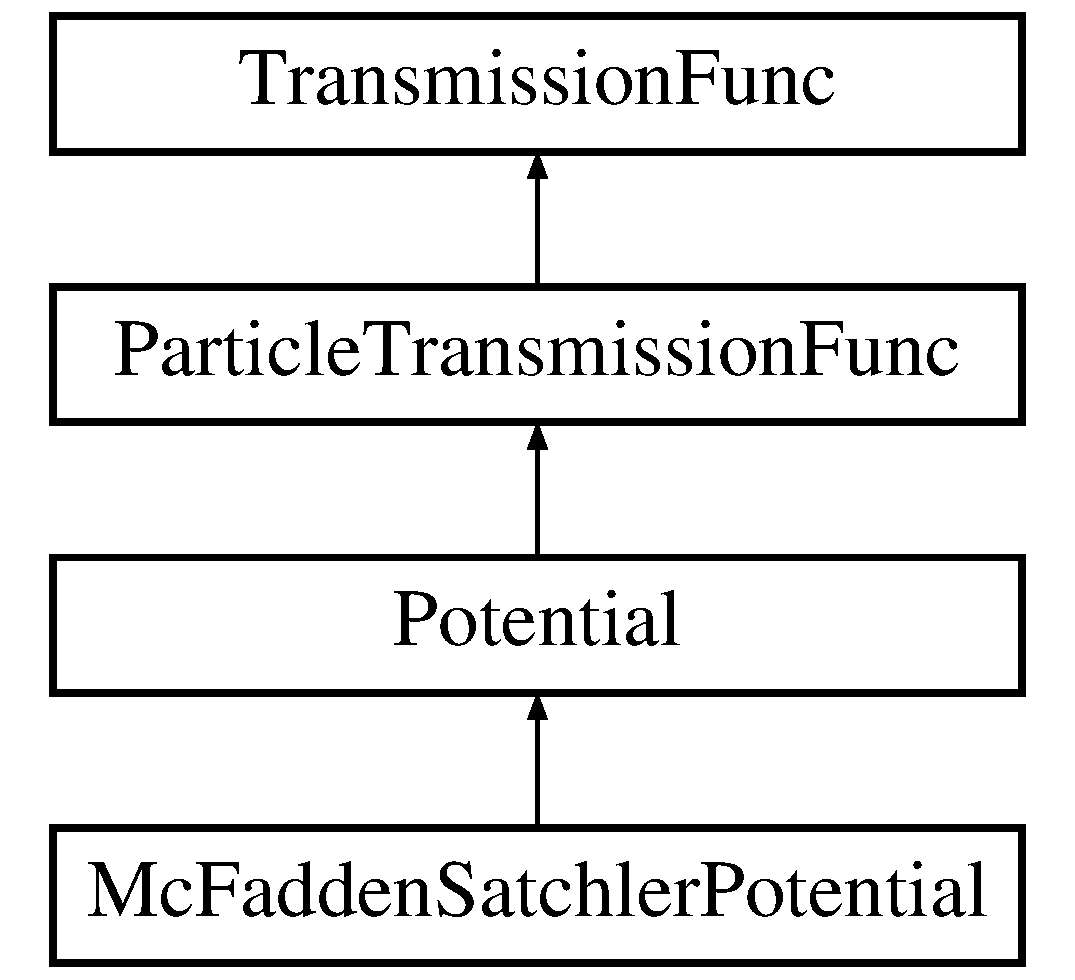
\includegraphics[height=4.000000cm]{da/d23/classMcFaddenSatchlerPotential}
\end{center}
\end{figure}
\subsection*{Public Member Functions}
\begin{DoxyCompactItemize}
\item 
\hyperlink{classMcFaddenSatchlerPotential_a24246503ca1d2d9931e93b00099e1577}{Mc\-Fadden\-Satchler\-Potential} (int, int, int, int, double, int, double, int, double, int, double, double, double, double, \hyperlink{classTransmissionFunc}{Transmission\-Func} $\ast$)
\item 
\hyperlink{Constants_8h_a1c1b16cc02d518bbe753449171ab7033}{std\-::complex}$<$ double $>$ \hyperlink{classMcFaddenSatchlerPotential_abbdff953b8577365fc0b60844d51ea4b}{Calculate} (double, int, double, double, double) const 
\end{DoxyCompactItemize}
\subsection*{Additional Inherited Members}


\subsection{Constructor \& Destructor Documentation}
\hypertarget{classMcFaddenSatchlerPotential_a24246503ca1d2d9931e93b00099e1577}{\index{Mc\-Fadden\-Satchler\-Potential@{Mc\-Fadden\-Satchler\-Potential}!Mc\-Fadden\-Satchler\-Potential@{Mc\-Fadden\-Satchler\-Potential}}
\index{Mc\-Fadden\-Satchler\-Potential@{Mc\-Fadden\-Satchler\-Potential}!McFaddenSatchlerPotential@{Mc\-Fadden\-Satchler\-Potential}}
\subsubsection[{Mc\-Fadden\-Satchler\-Potential}]{\setlength{\rightskip}{0pt plus 5cm}Mc\-Fadden\-Satchler\-Potential\-::\-Mc\-Fadden\-Satchler\-Potential (
\begin{DoxyParamCaption}
\item[{int}]{z1, }
\item[{int}]{m1, }
\item[{int}]{z2, }
\item[{int}]{m2, }
\item[{double}]{j\-Initial, }
\item[{int}]{pi\-Initial, }
\item[{double}]{j\-Final, }
\item[{int}]{pi\-Final, }
\item[{double}]{spin, }
\item[{int}]{parity, }
\item[{double}]{max\-L, }
\item[{double}]{total\-Width\-For\-Correction, }
\item[{double}]{uncorr\-Total\-Width\-For\-Correction, }
\item[{double}]{uncorr\-Total\-Width\-Sqrd\-For\-Correction, }
\item[{{\bf Transmission\-Func} $\ast$}]{previous}
\end{DoxyParamCaption}
)}}\label{classMcFaddenSatchlerPotential_a24246503ca1d2d9931e93b00099e1577}


References Potential\-::boundary\-Radius\-\_\-, Potential\-::coulomb\-Radius\-\_\-, and Transmission\-Func\-::m2\-\_\-.



\subsection{Member Function Documentation}
\hypertarget{classMcFaddenSatchlerPotential_abbdff953b8577365fc0b60844d51ea4b}{\index{Mc\-Fadden\-Satchler\-Potential@{Mc\-Fadden\-Satchler\-Potential}!Calculate@{Calculate}}
\index{Calculate@{Calculate}!McFaddenSatchlerPotential@{Mc\-Fadden\-Satchler\-Potential}}
\subsubsection[{Calculate}]{\setlength{\rightskip}{0pt plus 5cm}{\bf std\-::complex}$<$ double $>$ Mc\-Fadden\-Satchler\-Potential\-::\-Calculate (
\begin{DoxyParamCaption}
\item[{double}]{r, }
\item[{int}]{l, }
\item[{double}]{s, }
\item[{double}]{j, }
\item[{double}]{energy}
\end{DoxyParamCaption}
) const\hspace{0.3cm}{\ttfamily [virtual]}}}\label{classMcFaddenSatchlerPotential_abbdff953b8577365fc0b60844d51ea4b}


Implements \hyperlink{classPotential_af6d2217c4a1f91e7ebb84d5b728d11aa}{Potential}.



References Potential\-::coulomb\-Radius\-\_\-, fstruc, Potential\-::\-Get\-Z1\-Z2(), and hbarc.



The documentation for this class was generated from the following files\-:\begin{DoxyCompactItemize}
\item 
include/\hyperlink{McFaddenSatchlerPotential_8h}{Mc\-Fadden\-Satchler\-Potential.\-h}\item 
src/\hyperlink{McFaddenSatchlerPotential_8cpp}{Mc\-Fadden\-Satchler\-Potential.\-cpp}\end{DoxyCompactItemize}

\hypertarget{classNuclearLevels}{\section{Nuclear\-Levels Class Reference}
\label{classNuclearLevels}\index{Nuclear\-Levels@{Nuclear\-Levels}}
}


{\ttfamily \#include $<$Nuclear\-Levels.\-h$>$}

\subsection*{Static Public Member Functions}
\begin{DoxyCompactItemize}
\item 
static void \hyperlink{classNuclearLevels_aa1ab44bf4eb60e689aaa859fdd3c1d74}{Initialize\-Levels} (std\-::string levels\-Directory, std\-::string spin\-File)
\item 
static void \hyperlink{classNuclearLevels_a0b1e703bb57ace97c694496f71fe5cf9}{Print\-Levels} (int, int)
\item 
static std\-::vector$<$ \hyperlink{classLevel}{Level} $>$ \hyperlink{classNuclearLevels_a5e8207a4e5c77fcfca70482f9a4c6541}{Find\-Levels} (int, int)
\end{DoxyCompactItemize}


\subsection{Member Function Documentation}
\hypertarget{classNuclearLevels_a5e8207a4e5c77fcfca70482f9a4c6541}{\index{Nuclear\-Levels@{Nuclear\-Levels}!Find\-Levels@{Find\-Levels}}
\index{Find\-Levels@{Find\-Levels}!NuclearLevels@{Nuclear\-Levels}}
\subsubsection[{Find\-Levels}]{\setlength{\rightskip}{0pt plus 5cm}std\-::vector$<$ {\bf Level} $>$ Nuclear\-Levels\-::\-Find\-Levels (
\begin{DoxyParamCaption}
\item[{int}]{Z, }
\item[{int}]{A}
\end{DoxyParamCaption}
)\hspace{0.3cm}{\ttfamily [static]}}}\label{classNuclearLevels_a5e8207a4e5c77fcfca70482f9a4c6541}


Referenced by Cross\-Section\-::\-Cross\-Section(), Decayer\-::\-Decayer(), and Transition\-Rate\-Func\-::\-Transition\-Rate\-Func().

\hypertarget{classNuclearLevels_aa1ab44bf4eb60e689aaa859fdd3c1d74}{\index{Nuclear\-Levels@{Nuclear\-Levels}!Initialize\-Levels@{Initialize\-Levels}}
\index{Initialize\-Levels@{Initialize\-Levels}!NuclearLevels@{Nuclear\-Levels}}
\subsubsection[{Initialize\-Levels}]{\setlength{\rightskip}{0pt plus 5cm}void Nuclear\-Levels\-::\-Initialize\-Levels (
\begin{DoxyParamCaption}
\item[{std\-::string}]{levels\-Directory, }
\item[{std\-::string}]{spin\-File}
\end{DoxyParamCaption}
)\hspace{0.3cm}{\ttfamily [static]}}}\label{classNuclearLevels_aa1ab44bf4eb60e689aaa859fdd3c1d74}


References Levels\-Container\-::levels\-\_\-.



Referenced by Initialize().

\hypertarget{classNuclearLevels_a0b1e703bb57ace97c694496f71fe5cf9}{\index{Nuclear\-Levels@{Nuclear\-Levels}!Print\-Levels@{Print\-Levels}}
\index{Print\-Levels@{Print\-Levels}!NuclearLevels@{Nuclear\-Levels}}
\subsubsection[{Print\-Levels}]{\setlength{\rightskip}{0pt plus 5cm}void Nuclear\-Levels\-::\-Print\-Levels (
\begin{DoxyParamCaption}
\item[{int}]{Z, }
\item[{int}]{A}
\end{DoxyParamCaption}
)\hspace{0.3cm}{\ttfamily [static]}}}\label{classNuclearLevels_a0b1e703bb57ace97c694496f71fe5cf9}


The documentation for this class was generated from the following files\-:\begin{DoxyCompactItemize}
\item 
include/\hyperlink{NuclearLevels_8h}{Nuclear\-Levels.\-h}\item 
src/\hyperlink{NuclearLevels_8cpp}{Nuclear\-Levels.\-cpp}\item 
src/\hyperlink{Setup_8cpp}{Setup.\-cpp}\end{DoxyCompactItemize}

\hypertarget{classNuclearMass}{\section{Nuclear\-Mass Class Reference}
\label{classNuclearMass}\index{Nuclear\-Mass@{Nuclear\-Mass}}
}


{\ttfamily \#include $<$Nuclear\-Mass.\-h$>$}

\subsection*{Static Public Member Functions}
\begin{DoxyCompactItemize}
\item 
static void \hyperlink{classNuclearMass_a7225a76222f0dd2e466092ef1e5f40dd}{Initialize\-Elements} ()
\item 
static void \hyperlink{classNuclearMass_a76145d2def7d6cd40b9524ab9518eff3}{Initialize\-Masses} (std\-::string)
\item 
static int \hyperlink{classNuclearMass_ae5b0875835707ce2567529cf88fe33b1}{Find\-Z} (std\-::string)
\item 
static std\-::string \hyperlink{classNuclearMass_aaffdbd2dabf1b1216763c32cf0a22a72}{Find\-Element} (int)
\item 
static bool \hyperlink{classNuclearMass_a3bf04f82484549832925bf4f2441466d}{Find\-Mass} (int, int, double \&)
\item 
static bool \hyperlink{classNuclearMass_a851078a4e77d62f2f272e84bff5a4ee5}{Mass\-Difference} (int, int, int, int, double \&)
\item 
static bool \hyperlink{classNuclearMass_a6086c9b206e6a63c9895f7cdd954d5e8}{Q\-Value} (int, int, int, int, double \&)
\item 
static bool \hyperlink{classNuclearMass_acea701823ae741db56e908cf0910d3f1}{Neutron\-Pairing\-Gap} (int, int, double \&)
\item 
static bool \hyperlink{classNuclearMass_ab85a213db514601c61cf1f00a307e3ea}{Proton\-Pairing\-Gap} (int, int, double \&)
\item 
static bool \hyperlink{classNuclearMass_a6d1e15e3b55000fee7dcd9d12a983793}{Micro\-Energy\-Corr} (int, int, double \&)
\item 
static bool \hyperlink{classNuclearMass_acac25b099886be862e5e5bf40a6f16ef}{Highest\-Bound\-Energy} (int, int, double \&)
\item 
static double \hyperlink{classNuclearMass_a1e07c46a9d3b0f4338b23e8c0f7db99b}{Calculate\-L\-D\-M\-Mass} (int, int)
\end{DoxyCompactItemize}


\subsection{Member Function Documentation}
\hypertarget{classNuclearMass_a1e07c46a9d3b0f4338b23e8c0f7db99b}{\index{Nuclear\-Mass@{Nuclear\-Mass}!Calculate\-L\-D\-M\-Mass@{Calculate\-L\-D\-M\-Mass}}
\index{Calculate\-L\-D\-M\-Mass@{Calculate\-L\-D\-M\-Mass}!NuclearMass@{Nuclear\-Mass}}
\subsubsection[{Calculate\-L\-D\-M\-Mass}]{\setlength{\rightskip}{0pt plus 5cm}double Nuclear\-Mass\-::\-Calculate\-L\-D\-M\-Mass (
\begin{DoxyParamCaption}
\item[{int}]{Z, }
\item[{int}]{A}
\end{DoxyParamCaption}
)\hspace{0.3cm}{\ttfamily [static]}}}\label{classNuclearMass_a1e07c46a9d3b0f4338b23e8c0f7db99b}
Calculates liquid drop model mass based on T\-A\-L\-Y\-S parametrization. 

References uconv.

\hypertarget{classNuclearMass_aaffdbd2dabf1b1216763c32cf0a22a72}{\index{Nuclear\-Mass@{Nuclear\-Mass}!Find\-Element@{Find\-Element}}
\index{Find\-Element@{Find\-Element}!NuclearMass@{Nuclear\-Mass}}
\subsubsection[{Find\-Element}]{\setlength{\rightskip}{0pt plus 5cm}std\-::string Nuclear\-Mass\-::\-Find\-Element (
\begin{DoxyParamCaption}
\item[{int}]{Z}
\end{DoxyParamCaption}
)\hspace{0.3cm}{\ttfamily [static]}}}\label{classNuclearMass_aaffdbd2dabf1b1216763c32cf0a22a72}


Referenced by Decay\-Results\-::\-Decay\-Results(), Cross\-Section\-::\-Print\-Cross\-Sections(), Cross\-Section\-::\-Print\-Reaction\-Rates(), and Cross\-Section\-::\-Print\-Transmission\-Terms().

\hypertarget{classNuclearMass_a3bf04f82484549832925bf4f2441466d}{\index{Nuclear\-Mass@{Nuclear\-Mass}!Find\-Mass@{Find\-Mass}}
\index{Find\-Mass@{Find\-Mass}!NuclearMass@{Nuclear\-Mass}}
\subsubsection[{Find\-Mass}]{\setlength{\rightskip}{0pt plus 5cm}bool Nuclear\-Mass\-::\-Find\-Mass (
\begin{DoxyParamCaption}
\item[{int}]{Z, }
\item[{int}]{A, }
\item[{double \&}]{M}
\end{DoxyParamCaption}
)\hspace{0.3cm}{\ttfamily [static]}}}\label{classNuclearMass_a3bf04f82484549832925bf4f2441466d}


References H\-A\-S\-\_\-\-E\-X\-P\-\_\-\-M\-A\-S\-S, and H\-A\-S\-\_\-\-T\-H\-\_\-\-M\-A\-S\-S.



Referenced by Gamma\-Transmission\-Func\-::\-Gamma\-Transmission\-Func(), Mass\-Difference(), Particle\-Transmission\-Func\-::\-Particle\-Transmission\-Func(), and Q\-Value().

\hypertarget{classNuclearMass_ae5b0875835707ce2567529cf88fe33b1}{\index{Nuclear\-Mass@{Nuclear\-Mass}!Find\-Z@{Find\-Z}}
\index{Find\-Z@{Find\-Z}!NuclearMass@{Nuclear\-Mass}}
\subsubsection[{Find\-Z}]{\setlength{\rightskip}{0pt plus 5cm}int Nuclear\-Mass\-::\-Find\-Z (
\begin{DoxyParamCaption}
\item[{std\-::string}]{element}
\end{DoxyParamCaption}
)\hspace{0.3cm}{\ttfamily [static]}}}\label{classNuclearMass_ae5b0875835707ce2567529cf88fe33b1}


Referenced by parse\-Command\-Line\-For\-Decay(), and parse\-Command\-Line\-For\-X\-S().

\hypertarget{classNuclearMass_acac25b099886be862e5e5bf40a6f16ef}{\index{Nuclear\-Mass@{Nuclear\-Mass}!Highest\-Bound\-Energy@{Highest\-Bound\-Energy}}
\index{Highest\-Bound\-Energy@{Highest\-Bound\-Energy}!NuclearMass@{Nuclear\-Mass}}
\subsubsection[{Highest\-Bound\-Energy}]{\setlength{\rightskip}{0pt plus 5cm}bool Nuclear\-Mass\-::\-Highest\-Bound\-Energy (
\begin{DoxyParamCaption}
\item[{int}]{Z, }
\item[{int}]{A, }
\item[{double \&}]{energy}
\end{DoxyParamCaption}
)\hspace{0.3cm}{\ttfamily [static]}}}\label{classNuclearMass_acac25b099886be862e5e5bf40a6f16ef}


References Q\-Value().



Referenced by Transition\-Rate\-Func\-::\-Transition\-Rate\-Func().

\hypertarget{classNuclearMass_a7225a76222f0dd2e466092ef1e5f40dd}{\index{Nuclear\-Mass@{Nuclear\-Mass}!Initialize\-Elements@{Initialize\-Elements}}
\index{Initialize\-Elements@{Initialize\-Elements}!NuclearMass@{Nuclear\-Mass}}
\subsubsection[{Initialize\-Elements}]{\setlength{\rightskip}{0pt plus 5cm}void Nuclear\-Mass\-::\-Initialize\-Elements (
\begin{DoxyParamCaption}
{}
\end{DoxyParamCaption}
)\hspace{0.3cm}{\ttfamily [static]}}}\label{classNuclearMass_a7225a76222f0dd2e466092ef1e5f40dd}


Referenced by Initialize().

\hypertarget{classNuclearMass_a76145d2def7d6cd40b9524ab9518eff3}{\index{Nuclear\-Mass@{Nuclear\-Mass}!Initialize\-Masses@{Initialize\-Masses}}
\index{Initialize\-Masses@{Initialize\-Masses}!NuclearMass@{Nuclear\-Mass}}
\subsubsection[{Initialize\-Masses}]{\setlength{\rightskip}{0pt plus 5cm}void Nuclear\-Mass\-::\-Initialize\-Masses (
\begin{DoxyParamCaption}
\item[{std\-::string}]{filename}
\end{DoxyParamCaption}
)\hspace{0.3cm}{\ttfamily [static]}}}\label{classNuclearMass_a76145d2def7d6cd40b9524ab9518eff3}


References H\-A\-S\-\_\-\-E\-X\-P\-\_\-\-M\-A\-S\-S, H\-A\-S\-\_\-\-T\-H\-\_\-\-M\-A\-S\-S, and uconv.



Referenced by Initialize().

\hypertarget{classNuclearMass_a851078a4e77d62f2f272e84bff5a4ee5}{\index{Nuclear\-Mass@{Nuclear\-Mass}!Mass\-Difference@{Mass\-Difference}}
\index{Mass\-Difference@{Mass\-Difference}!NuclearMass@{Nuclear\-Mass}}
\subsubsection[{Mass\-Difference}]{\setlength{\rightskip}{0pt plus 5cm}bool Nuclear\-Mass\-::\-Mass\-Difference (
\begin{DoxyParamCaption}
\item[{int}]{Z1, }
\item[{int}]{A1, }
\item[{int}]{Z2, }
\item[{int}]{A2, }
\item[{double \&}]{difference}
\end{DoxyParamCaption}
)\hspace{0.3cm}{\ttfamily [static]}}}\label{classNuclearMass_a851078a4e77d62f2f272e84bff5a4ee5}


References Find\-Mass().



Referenced by Neutron\-Pairing\-Gap(), Proton\-Pairing\-Gap(), and Q\-Value().

\hypertarget{classNuclearMass_a6d1e15e3b55000fee7dcd9d12a983793}{\index{Nuclear\-Mass@{Nuclear\-Mass}!Micro\-Energy\-Corr@{Micro\-Energy\-Corr}}
\index{Micro\-Energy\-Corr@{Micro\-Energy\-Corr}!NuclearMass@{Nuclear\-Mass}}
\subsubsection[{Micro\-Energy\-Corr}]{\setlength{\rightskip}{0pt plus 5cm}bool Nuclear\-Mass\-::\-Micro\-Energy\-Corr (
\begin{DoxyParamCaption}
\item[{int}]{Z, }
\item[{int}]{A, }
\item[{double \&}]{correction}
\end{DoxyParamCaption}
)\hspace{0.3cm}{\ttfamily [static]}}}\label{classNuclearMass_a6d1e15e3b55000fee7dcd9d12a983793}


Referenced by Rauscher\-Level\-Density\-::\-Rauscher\-Level\-Density().

\hypertarget{classNuclearMass_acea701823ae741db56e908cf0910d3f1}{\index{Nuclear\-Mass@{Nuclear\-Mass}!Neutron\-Pairing\-Gap@{Neutron\-Pairing\-Gap}}
\index{Neutron\-Pairing\-Gap@{Neutron\-Pairing\-Gap}!NuclearMass@{Nuclear\-Mass}}
\subsubsection[{Neutron\-Pairing\-Gap}]{\setlength{\rightskip}{0pt plus 5cm}bool Nuclear\-Mass\-::\-Neutron\-Pairing\-Gap (
\begin{DoxyParamCaption}
\item[{int}]{Z, }
\item[{int}]{A, }
\item[{double \&}]{pairing\-Gap}
\end{DoxyParamCaption}
)\hspace{0.3cm}{\ttfamily [static]}}}\label{classNuclearMass_acea701823ae741db56e908cf0910d3f1}


References Mass\-Difference().



Referenced by Rauscher\-Level\-Density\-::\-Calc\-Back\-Shift().

\hypertarget{classNuclearMass_ab85a213db514601c61cf1f00a307e3ea}{\index{Nuclear\-Mass@{Nuclear\-Mass}!Proton\-Pairing\-Gap@{Proton\-Pairing\-Gap}}
\index{Proton\-Pairing\-Gap@{Proton\-Pairing\-Gap}!NuclearMass@{Nuclear\-Mass}}
\subsubsection[{Proton\-Pairing\-Gap}]{\setlength{\rightskip}{0pt plus 5cm}bool Nuclear\-Mass\-::\-Proton\-Pairing\-Gap (
\begin{DoxyParamCaption}
\item[{int}]{Z, }
\item[{int}]{A, }
\item[{double \&}]{pairing\-Gap}
\end{DoxyParamCaption}
)\hspace{0.3cm}{\ttfamily [static]}}}\label{classNuclearMass_ab85a213db514601c61cf1f00a307e3ea}


References Mass\-Difference().



Referenced by Rauscher\-Level\-Density\-::\-Calc\-Back\-Shift().

\hypertarget{classNuclearMass_a6086c9b206e6a63c9895f7cdd954d5e8}{\index{Nuclear\-Mass@{Nuclear\-Mass}!Q\-Value@{Q\-Value}}
\index{Q\-Value@{Q\-Value}!NuclearMass@{Nuclear\-Mass}}
\subsubsection[{Q\-Value}]{\setlength{\rightskip}{0pt plus 5cm}bool Nuclear\-Mass\-::\-Q\-Value (
\begin{DoxyParamCaption}
\item[{int}]{Z1, }
\item[{int}]{A1, }
\item[{int}]{Z2, }
\item[{int}]{A2, }
\item[{double \&}]{q\-Value}
\end{DoxyParamCaption}
)\hspace{0.3cm}{\ttfamily [static]}}}\label{classNuclearMass_a6086c9b206e6a63c9895f7cdd954d5e8}


References Find\-Mass(), and Mass\-Difference().



Referenced by Cross\-Section\-::\-Cross\-Section(), Decayer\-::\-Decayer(), Highest\-Bound\-Energy(), Kopecky\-Uhl\-G\-S\-F\-::\-Kopecky\-Uhl\-G\-S\-F(), Particle\-Hole\-Level\-Density\-::\-Particle\-Hole\-Level\-Density(), and Pre\-Eq\-Decayer\-::\-Pre\-Eq\-Decayer().



The documentation for this class was generated from the following files\-:\begin{DoxyCompactItemize}
\item 
include/\hyperlink{NuclearMass_8h}{Nuclear\-Mass.\-h}\item 
src/\hyperlink{NuclearMass_8cpp}{Nuclear\-Mass.\-cpp}\item 
src/\hyperlink{Setup_8cpp}{Setup.\-cpp}\end{DoxyCompactItemize}

\hypertarget{classODE__integration}{\section{O\-D\-E\-\_\-integration Class Reference}
\label{classODE__integration}\index{O\-D\-E\-\_\-integration@{O\-D\-E\-\_\-integration}}
}


{\ttfamily \#include $<$ode\-\_\-int.\-H$>$}

\subsection*{Public Member Functions}
\begin{DoxyCompactItemize}
\item 
\hyperlink{classODE__integration_afc5a3b1e8449627f4d810686345814b2}{O\-D\-E\-\_\-integration} (const \hyperlink{Constants_8h_a1c1b16cc02d518bbe753449171ab7033}{std\-::complex}$<$ double $>$ \&l\-\_\-1, const \hyperlink{Constants_8h_a1c1b16cc02d518bbe753449171ab7033}{std\-::complex}$<$ double $>$ \&two\-\_\-eta\-\_\-1)
\item 
void \hyperlink{classODE__integration_a9806108275553b175071e0f4306c0729}{operator()} (const \hyperlink{Constants_8h_a1c1b16cc02d518bbe753449171ab7033}{std\-::complex}$<$ double $>$ \&r0, const \hyperlink{Constants_8h_a1c1b16cc02d518bbe753449171ab7033}{std\-::complex}$<$ double $>$ \&u0, const \hyperlink{Constants_8h_a1c1b16cc02d518bbe753449171ab7033}{std\-::complex}$<$ double $>$ \&du0, const \hyperlink{Constants_8h_a1c1b16cc02d518bbe753449171ab7033}{std\-::complex}$<$ double $>$ \&r, \hyperlink{Constants_8h_a1c1b16cc02d518bbe753449171ab7033}{std\-::complex}$<$ double $>$ \&u, \hyperlink{Constants_8h_a1c1b16cc02d518bbe753449171ab7033}{std\-::complex}$<$ double $>$ \&du) const 
\end{DoxyCompactItemize}


\subsection{Constructor \& Destructor Documentation}
\hypertarget{classODE__integration_afc5a3b1e8449627f4d810686345814b2}{\index{O\-D\-E\-\_\-integration@{O\-D\-E\-\_\-integration}!O\-D\-E\-\_\-integration@{O\-D\-E\-\_\-integration}}
\index{O\-D\-E\-\_\-integration@{O\-D\-E\-\_\-integration}!ODE_integration@{O\-D\-E\-\_\-integration}}
\subsubsection[{O\-D\-E\-\_\-integration}]{\setlength{\rightskip}{0pt plus 5cm}O\-D\-E\-\_\-integration\-::\-O\-D\-E\-\_\-integration (
\begin{DoxyParamCaption}
\item[{const {\bf std\-::complex}$<$ double $>$ \&}]{l\-\_\-1, }
\item[{const {\bf std\-::complex}$<$ double $>$ \&}]{two\-\_\-eta\-\_\-1}
\end{DoxyParamCaption}
)\hspace{0.3cm}{\ttfamily [inline]}}}\label{classODE__integration_afc5a3b1e8449627f4d810686345814b2}


\subsection{Member Function Documentation}
\hypertarget{classODE__integration_a9806108275553b175071e0f4306c0729}{\index{O\-D\-E\-\_\-integration@{O\-D\-E\-\_\-integration}!operator()@{operator()}}
\index{operator()@{operator()}!ODE_integration@{O\-D\-E\-\_\-integration}}
\subsubsection[{operator()}]{\setlength{\rightskip}{0pt plus 5cm}void O\-D\-E\-\_\-integration\-::operator() (
\begin{DoxyParamCaption}
\item[{const {\bf std\-::complex}$<$ double $>$ \&}]{r0, }
\item[{const {\bf std\-::complex}$<$ double $>$ \&}]{u0, }
\item[{const {\bf std\-::complex}$<$ double $>$ \&}]{du0, }
\item[{const {\bf std\-::complex}$<$ double $>$ \&}]{r, }
\item[{{\bf std\-::complex}$<$ double $>$ \&}]{u, }
\item[{{\bf std\-::complex}$<$ double $>$ \&}]{du}
\end{DoxyParamCaption}
) const}}\label{classODE__integration_a9806108275553b175071e0f4306c0729}


References inf\-\_\-norm(), and precision.



The documentation for this class was generated from the following files\-:\begin{DoxyCompactItemize}
\item 
/afs/crc.\-nd.\-edu/user/p/pscholz/\-Private/sapphire-\/devel/coul/include/\hyperlink{ode__int_8H}{ode\-\_\-int.\-H}\item 
/afs/crc.\-nd.\-edu/user/p/pscholz/\-Private/sapphire-\/devel/coul/src/\hyperlink{ode__int_8cpp}{ode\-\_\-int.\-cpp}\end{DoxyCompactItemize}

\hypertarget{classParticleHoleLevelDensity}{\section{Particle\-Hole\-Level\-Density Class Reference}
\label{classParticleHoleLevelDensity}\index{Particle\-Hole\-Level\-Density@{Particle\-Hole\-Level\-Density}}
}


{\ttfamily \#include $<$Particle\-Hole\-Level\-Density.\-h$>$}

\subsection*{Public Member Functions}
\begin{DoxyCompactItemize}
\item 
\hyperlink{classParticleHoleLevelDensity_a47725bc4322c23076475bc4f729c4993}{Particle\-Hole\-Level\-Density} (int, int, double, int, int, int, int)
\item 
double \hyperlink{classParticleHoleLevelDensity_a9529125c1d9a033b46ceab05259cfa26}{operator()} (double energy, bool correct=true, bool spin=false)
\item 
double \hyperlink{classParticleHoleLevelDensity_a7b3aa8776f1913453389e6fd6172e216}{Pauli\-Correction} (int, int, int, int)
\item 
double \hyperlink{classParticleHoleLevelDensity_ac9719244be6c45a25b5dfe208c363bbd}{Pairing\-Correction} (double energy)
\item 
double \hyperlink{classParticleHoleLevelDensity_af990f31da2a0bab282762bffea976586}{g\-Nu} () const 
\item 
double \hyperlink{classParticleHoleLevelDensity_a2f46edfdc4a2c8257dd6a2ca5ef573b1}{g\-Pi} () const 
\item 
double \hyperlink{classParticleHoleLevelDensity_a162ffe8a3e56cca1c3ffc6bc13f45254}{Finite\-Depth} (double)
\end{DoxyCompactItemize}


\subsection{Constructor \& Destructor Documentation}
\hypertarget{classParticleHoleLevelDensity_a47725bc4322c23076475bc4f729c4993}{\index{Particle\-Hole\-Level\-Density@{Particle\-Hole\-Level\-Density}!Particle\-Hole\-Level\-Density@{Particle\-Hole\-Level\-Density}}
\index{Particle\-Hole\-Level\-Density@{Particle\-Hole\-Level\-Density}!ParticleHoleLevelDensity@{Particle\-Hole\-Level\-Density}}
\subsubsection[{Particle\-Hole\-Level\-Density}]{\setlength{\rightskip}{0pt plus 5cm}Particle\-Hole\-Level\-Density\-::\-Particle\-Hole\-Level\-Density (
\begin{DoxyParamCaption}
\item[{int}]{Z, }
\item[{int}]{A, }
\item[{double}]{J, }
\item[{int}]{neutron\-Number, }
\item[{int}]{neutron\-Hole\-Number, }
\item[{int}]{proton\-Number, }
\item[{int}]{proton\-Hole\-Number}
\end{DoxyParamCaption}
)}}\label{classParticleHoleLevelDensity_a47725bc4322c23076475bc4f729c4993}


References Pauli\-Correction(), and Nuclear\-Mass\-::\-Q\-Value().



\subsection{Member Function Documentation}
\hypertarget{classParticleHoleLevelDensity_a162ffe8a3e56cca1c3ffc6bc13f45254}{\index{Particle\-Hole\-Level\-Density@{Particle\-Hole\-Level\-Density}!Finite\-Depth@{Finite\-Depth}}
\index{Finite\-Depth@{Finite\-Depth}!ParticleHoleLevelDensity@{Particle\-Hole\-Level\-Density}}
\subsubsection[{Finite\-Depth}]{\setlength{\rightskip}{0pt plus 5cm}double Particle\-Hole\-Level\-Density\-::\-Finite\-Depth (
\begin{DoxyParamCaption}
\item[{double}]{energy}
\end{DoxyParamCaption}
)}}\label{classParticleHoleLevelDensity_a162ffe8a3e56cca1c3ffc6bc13f45254}


Referenced by operator()().

\hypertarget{classParticleHoleLevelDensity_af990f31da2a0bab282762bffea976586}{\index{Particle\-Hole\-Level\-Density@{Particle\-Hole\-Level\-Density}!g\-Nu@{g\-Nu}}
\index{g\-Nu@{g\-Nu}!ParticleHoleLevelDensity@{Particle\-Hole\-Level\-Density}}
\subsubsection[{g\-Nu}]{\setlength{\rightskip}{0pt plus 5cm}double Particle\-Hole\-Level\-Density\-::g\-Nu (
\begin{DoxyParamCaption}
{}
\end{DoxyParamCaption}
) const\hspace{0.3cm}{\ttfamily [inline]}}}\label{classParticleHoleLevelDensity_af990f31da2a0bab282762bffea976586}
\hypertarget{classParticleHoleLevelDensity_a2f46edfdc4a2c8257dd6a2ca5ef573b1}{\index{Particle\-Hole\-Level\-Density@{Particle\-Hole\-Level\-Density}!g\-Pi@{g\-Pi}}
\index{g\-Pi@{g\-Pi}!ParticleHoleLevelDensity@{Particle\-Hole\-Level\-Density}}
\subsubsection[{g\-Pi}]{\setlength{\rightskip}{0pt plus 5cm}double Particle\-Hole\-Level\-Density\-::g\-Pi (
\begin{DoxyParamCaption}
{}
\end{DoxyParamCaption}
) const\hspace{0.3cm}{\ttfamily [inline]}}}\label{classParticleHoleLevelDensity_a2f46edfdc4a2c8257dd6a2ca5ef573b1}
\hypertarget{classParticleHoleLevelDensity_a9529125c1d9a033b46ceab05259cfa26}{\index{Particle\-Hole\-Level\-Density@{Particle\-Hole\-Level\-Density}!operator()@{operator()}}
\index{operator()@{operator()}!ParticleHoleLevelDensity@{Particle\-Hole\-Level\-Density}}
\subsubsection[{operator()}]{\setlength{\rightskip}{0pt plus 5cm}double Particle\-Hole\-Level\-Density\-::operator() (
\begin{DoxyParamCaption}
\item[{double}]{energy, }
\item[{bool}]{correct = {\ttfamily true}, }
\item[{bool}]{spin = {\ttfamily false}}
\end{DoxyParamCaption}
)}}\label{classParticleHoleLevelDensity_a9529125c1d9a033b46ceab05259cfa26}


References Finite\-Depth(), and Pairing\-Correction().

\hypertarget{classParticleHoleLevelDensity_ac9719244be6c45a25b5dfe208c363bbd}{\index{Particle\-Hole\-Level\-Density@{Particle\-Hole\-Level\-Density}!Pairing\-Correction@{Pairing\-Correction}}
\index{Pairing\-Correction@{Pairing\-Correction}!ParticleHoleLevelDensity@{Particle\-Hole\-Level\-Density}}
\subsubsection[{Pairing\-Correction}]{\setlength{\rightskip}{0pt plus 5cm}double Particle\-Hole\-Level\-Density\-::\-Pairing\-Correction (
\begin{DoxyParamCaption}
\item[{double}]{energy}
\end{DoxyParamCaption}
)}}\label{classParticleHoleLevelDensity_ac9719244be6c45a25b5dfe208c363bbd}


Referenced by operator()().

\hypertarget{classParticleHoleLevelDensity_a7b3aa8776f1913453389e6fd6172e216}{\index{Particle\-Hole\-Level\-Density@{Particle\-Hole\-Level\-Density}!Pauli\-Correction@{Pauli\-Correction}}
\index{Pauli\-Correction@{Pauli\-Correction}!ParticleHoleLevelDensity@{Particle\-Hole\-Level\-Density}}
\subsubsection[{Pauli\-Correction}]{\setlength{\rightskip}{0pt plus 5cm}double Particle\-Hole\-Level\-Density\-::\-Pauli\-Correction (
\begin{DoxyParamCaption}
\item[{int}]{neutron\-Number, }
\item[{int}]{neutron\-Hole\-Number, }
\item[{int}]{proton\-Number, }
\item[{int}]{proton\-Hole\-Number}
\end{DoxyParamCaption}
)}}\label{classParticleHoleLevelDensity_a7b3aa8776f1913453389e6fd6172e216}


Referenced by Particle\-Hole\-Level\-Density().



The documentation for this class was generated from the following files\-:\begin{DoxyCompactItemize}
\item 
include/\hyperlink{ParticleHoleLevelDensity_8h}{Particle\-Hole\-Level\-Density.\-h}\item 
src/\hyperlink{ParticleHoleLevelDensity_8cpp}{Particle\-Hole\-Level\-Density.\-cpp}\end{DoxyCompactItemize}

\hypertarget{classParticleTransmissionFunc}{\section{Particle\-Transmission\-Func Class Reference}
\label{classParticleTransmissionFunc}\index{Particle\-Transmission\-Func@{Particle\-Transmission\-Func}}
}


{\ttfamily \#include $<$Particle\-Transmission\-Func.\-h$>$}

Inheritance diagram for Particle\-Transmission\-Func\-:\begin{figure}[H]
\begin{center}
\leavevmode
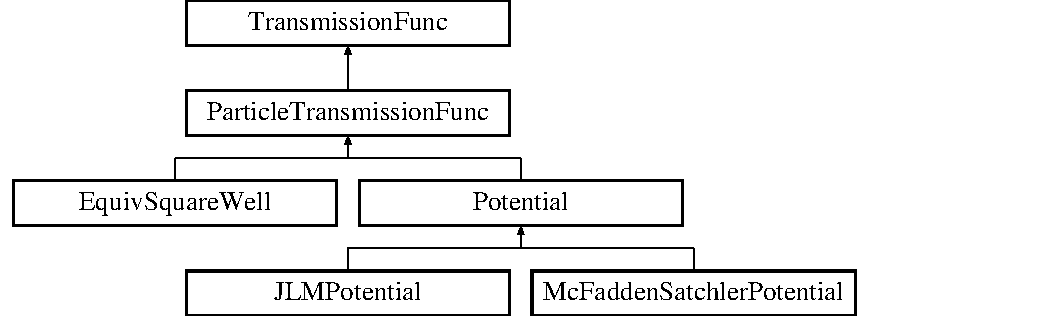
\includegraphics[height=4.000000cm]{d3/df3/classParticleTransmissionFunc}
\end{center}
\end{figure}
\subsection*{Public Member Functions}
\begin{DoxyCompactItemize}
\item 
\hyperlink{classParticleTransmissionFunc_a73fb78cabd594e804225c60fb6b1061f}{Particle\-Transmission\-Func} (int z1, int m1, int z2, int m2, double j\-Initial, int pi\-Initial, double j\-Final, int pi\-Final, double spin, int parity, double max\-L, double total\-Width\-For\-Correction, double uncorr\-Total\-Width\-For\-Correction, double uncorr\-Total\-Width\-Sqrd\-For\-Correction, \hyperlink{classTransmissionFunc}{Transmission\-Func} $\ast$previous)
\item 
virtual \hyperlink{classParticleTransmissionFunc_a9731c8c88dbd868583d286fb2a51df92}{$\sim$\-Particle\-Transmission\-Func} ()
\item 
bool \hyperlink{classParticleTransmissionFunc_a4bfae205a7c0fed1c590b4fd7f843443}{Is\-Valid} ()
\item 
double \hyperlink{classParticleTransmissionFunc_a9130fbae97d96592ae6d493607e801d4}{operator()} (double)
\item 
double \hyperlink{classParticleTransmissionFunc_aa9ae316a1b1d98084c88564b6faa5360}{operator()} (double, int)
\item 
void \hyperlink{classParticleTransmissionFunc_a0360cd28e5901a772c047d1893e6cb9d}{Calc\-S\-L\-Dependent\-Functions} (double, std\-::map$<$ \hyperlink{classSLPair}{S\-L\-Pair}, double $>$ \&)
\end{DoxyCompactItemize}
\subsection*{Static Public Member Functions}
\begin{DoxyCompactItemize}
\item 
static \hyperlink{classParticleTransmissionFunc}{Particle\-Transmission\-Func} $\ast$ \hyperlink{classParticleTransmissionFunc_a4293d27b31c6c32440483991b5dc5d23}{Create\-Particle\-Transmission\-Func} (int, int, int, int, double, int, double, int, double, int, double, double, double, double, \hyperlink{classTransmissionFunc}{Transmission\-Func} $\ast$)
\item 
static void \hyperlink{classParticleTransmissionFunc_a290c59558c005ef083796f2be9ee0edb}{Set\-Alpha\-Formalism} (int formalism)
\item 
static void \hyperlink{classParticleTransmissionFunc_aa4efea43e44552f5fdfc70b2203835af}{Set\-Neutron\-Formalism} (int formalism)
\item 
static void \hyperlink{classParticleTransmissionFunc_ad47eb7569638e7fec2af930bb624185b}{Set\-Proton\-Formalism} (int formalism)
\item 
static void \hyperlink{classParticleTransmissionFunc_a7a98d5b6d04b3fa31cc06e49bbcdf9f3}{Set\-Porter\-Thomas} (bool)
\end{DoxyCompactItemize}
\subsection*{Protected Member Functions}
\begin{DoxyCompactItemize}
\item 
virtual double \hyperlink{classParticleTransmissionFunc_a651cc8a1d96d72e12eaf66506c046856}{Calc\-Transmission} (double, int, double)=0
\end{DoxyCompactItemize}
\subsection*{Protected Attributes}
\begin{DoxyCompactItemize}
\item 
int \hyperlink{classParticleTransmissionFunc_a4c11b86051f613e37b10c692ea9746ce}{z1\-\_\-}
\item 
int \hyperlink{classParticleTransmissionFunc_ac63f83f460c222601d628856ed409a2b}{m1\-\_\-}
\item 
int \hyperlink{classParticleTransmissionFunc_a7d9ec139d40906290a13716e56412e23}{p\-Type\-\_\-}
\item 
int \hyperlink{classParticleTransmissionFunc_a3b5220600e09eeaec5bd1059fa1bd6b3}{parity\-\_\-}
\item 
double \hyperlink{classParticleTransmissionFunc_aa044907ae1f3827d8602fc33f4b0e92c}{redmass\-\_\-}
\item 
double \hyperlink{classParticleTransmissionFunc_a3143aef2c113158fca1643a2505f0b9a}{spin\-\_\-}
\end{DoxyCompactItemize}


\subsection{Constructor \& Destructor Documentation}
\hypertarget{classParticleTransmissionFunc_a73fb78cabd594e804225c60fb6b1061f}{\index{Particle\-Transmission\-Func@{Particle\-Transmission\-Func}!Particle\-Transmission\-Func@{Particle\-Transmission\-Func}}
\index{Particle\-Transmission\-Func@{Particle\-Transmission\-Func}!ParticleTransmissionFunc@{Particle\-Transmission\-Func}}
\subsubsection[{Particle\-Transmission\-Func}]{\setlength{\rightskip}{0pt plus 5cm}Particle\-Transmission\-Func\-::\-Particle\-Transmission\-Func (
\begin{DoxyParamCaption}
\item[{int}]{z1, }
\item[{int}]{m1, }
\item[{int}]{z2, }
\item[{int}]{m2, }
\item[{double}]{j\-Initial, }
\item[{int}]{pi\-Initial, }
\item[{double}]{j\-Final, }
\item[{int}]{pi\-Final, }
\item[{double}]{spin, }
\item[{int}]{parity, }
\item[{double}]{max\-L, }
\item[{double}]{total\-Width\-For\-Correction, }
\item[{double}]{uncorr\-Total\-Width\-For\-Correction, }
\item[{double}]{uncorr\-Total\-Width\-Sqrd\-For\-Correction, }
\item[{{\bf Transmission\-Func} $\ast$}]{previous}
\end{DoxyParamCaption}
)\hspace{0.3cm}{\ttfamily [inline]}}}\label{classParticleTransmissionFunc_a73fb78cabd594e804225c60fb6b1061f}


References Nuclear\-Mass\-::\-Find\-Mass(), m1\-\_\-, Transmission\-Func\-::m2\-\_\-, p\-Type\-\_\-, redmass\-\_\-, uconv, z1\-\_\-, and Transmission\-Func\-::z2\-\_\-.

\hypertarget{classParticleTransmissionFunc_a9731c8c88dbd868583d286fb2a51df92}{\index{Particle\-Transmission\-Func@{Particle\-Transmission\-Func}!$\sim$\-Particle\-Transmission\-Func@{$\sim$\-Particle\-Transmission\-Func}}
\index{$\sim$\-Particle\-Transmission\-Func@{$\sim$\-Particle\-Transmission\-Func}!ParticleTransmissionFunc@{Particle\-Transmission\-Func}}
\subsubsection[{$\sim$\-Particle\-Transmission\-Func}]{\setlength{\rightskip}{0pt plus 5cm}virtual Particle\-Transmission\-Func\-::$\sim$\-Particle\-Transmission\-Func (
\begin{DoxyParamCaption}
{}
\end{DoxyParamCaption}
)\hspace{0.3cm}{\ttfamily [inline]}, {\ttfamily [virtual]}}}\label{classParticleTransmissionFunc_a9731c8c88dbd868583d286fb2a51df92}


\subsection{Member Function Documentation}
\hypertarget{classParticleTransmissionFunc_a0360cd28e5901a772c047d1893e6cb9d}{\index{Particle\-Transmission\-Func@{Particle\-Transmission\-Func}!Calc\-S\-L\-Dependent\-Functions@{Calc\-S\-L\-Dependent\-Functions}}
\index{Calc\-S\-L\-Dependent\-Functions@{Calc\-S\-L\-Dependent\-Functions}!ParticleTransmissionFunc@{Particle\-Transmission\-Func}}
\subsubsection[{Calc\-S\-L\-Dependent\-Functions}]{\setlength{\rightskip}{0pt plus 5cm}void Particle\-Transmission\-Func\-::\-Calc\-S\-L\-Dependent\-Functions (
\begin{DoxyParamCaption}
\item[{double}]{energy, }
\item[{std\-::map$<$ {\bf S\-L\-Pair}, double $>$ \&}]{functions}
\end{DoxyParamCaption}
)}}\label{classParticleTransmissionFunc_a0360cd28e5901a772c047d1893e6cb9d}


References Calc\-Transmission(), Transmission\-Func\-::j\-Final\-\_\-, Transmission\-Func\-::j\-Initial\-\_\-, Transmission\-Func\-::max\-L\-\_\-, parity\-\_\-, Transmission\-Func\-::pi\-Final\-\_\-, Transmission\-Func\-::pi\-Initial\-\_\-, and spin\-\_\-.



Referenced by operator()().

\hypertarget{classParticleTransmissionFunc_a651cc8a1d96d72e12eaf66506c046856}{\index{Particle\-Transmission\-Func@{Particle\-Transmission\-Func}!Calc\-Transmission@{Calc\-Transmission}}
\index{Calc\-Transmission@{Calc\-Transmission}!ParticleTransmissionFunc@{Particle\-Transmission\-Func}}
\subsubsection[{Calc\-Transmission}]{\setlength{\rightskip}{0pt plus 5cm}virtual double Particle\-Transmission\-Func\-::\-Calc\-Transmission (
\begin{DoxyParamCaption}
\item[{double}]{, }
\item[{int}]{, }
\item[{double}]{}
\end{DoxyParamCaption}
)\hspace{0.3cm}{\ttfamily [protected]}, {\ttfamily [pure virtual]}}}\label{classParticleTransmissionFunc_a651cc8a1d96d72e12eaf66506c046856}


Implemented in \hyperlink{classEquivSquareWell_a3b8b7b435b5fcdac36118458ffd5ade8}{Equiv\-Square\-Well}, and \hyperlink{classPotential_aea8adb2a1783a79985621a899118c967}{Potential}.



Referenced by Calc\-S\-L\-Dependent\-Functions().

\hypertarget{classParticleTransmissionFunc_a4293d27b31c6c32440483991b5dc5d23}{\index{Particle\-Transmission\-Func@{Particle\-Transmission\-Func}!Create\-Particle\-Transmission\-Func@{Create\-Particle\-Transmission\-Func}}
\index{Create\-Particle\-Transmission\-Func@{Create\-Particle\-Transmission\-Func}!ParticleTransmissionFunc@{Particle\-Transmission\-Func}}
\subsubsection[{Create\-Particle\-Transmission\-Func}]{\setlength{\rightskip}{0pt plus 5cm}{\bf Particle\-Transmission\-Func} $\ast$ Particle\-Transmission\-Func\-::\-Create\-Particle\-Transmission\-Func (
\begin{DoxyParamCaption}
\item[{int}]{z1, }
\item[{int}]{m1, }
\item[{int}]{z2, }
\item[{int}]{m2, }
\item[{double}]{j\-Initial, }
\item[{int}]{pi\-Initial, }
\item[{double}]{j\-Final, }
\item[{int}]{pi\-Final, }
\item[{double}]{spin, }
\item[{int}]{parity, }
\item[{double}]{max\-L, }
\item[{double}]{total\-Width\-For\-Correction, }
\item[{double}]{uncorr\-Total\-Width\-For\-Correction, }
\item[{double}]{uncorr\-Total\-Width\-Sqrd\-For\-Correction, }
\item[{{\bf Transmission\-Func} $\ast$}]{previous}
\end{DoxyParamCaption}
)\hspace{0.3cm}{\ttfamily [static]}}}\label{classParticleTransmissionFunc_a4293d27b31c6c32440483991b5dc5d23}


Referenced by Transition\-Rate\-Func\-::\-Transition\-Rate\-Func().

\hypertarget{classParticleTransmissionFunc_a4bfae205a7c0fed1c590b4fd7f843443}{\index{Particle\-Transmission\-Func@{Particle\-Transmission\-Func}!Is\-Valid@{Is\-Valid}}
\index{Is\-Valid@{Is\-Valid}!ParticleTransmissionFunc@{Particle\-Transmission\-Func}}
\subsubsection[{Is\-Valid}]{\setlength{\rightskip}{0pt plus 5cm}bool Particle\-Transmission\-Func\-::\-Is\-Valid (
\begin{DoxyParamCaption}
{}
\end{DoxyParamCaption}
)\hspace{0.3cm}{\ttfamily [inline]}, {\ttfamily [virtual]}}}\label{classParticleTransmissionFunc_a4bfae205a7c0fed1c590b4fd7f843443}


Implements \hyperlink{classTransmissionFunc_a6dadf2b6cfc37d4c3da0f8ee2a1563af}{Transmission\-Func}.



References p\-Type\-\_\-, and redmass\-\_\-.

\hypertarget{classParticleTransmissionFunc_a9130fbae97d96592ae6d493607e801d4}{\index{Particle\-Transmission\-Func@{Particle\-Transmission\-Func}!operator()@{operator()}}
\index{operator()@{operator()}!ParticleTransmissionFunc@{Particle\-Transmission\-Func}}
\subsubsection[{operator()}]{\setlength{\rightskip}{0pt plus 5cm}double Particle\-Transmission\-Func\-::operator() (
\begin{DoxyParamCaption}
\item[{double}]{energy}
\end{DoxyParamCaption}
)\hspace{0.3cm}{\ttfamily [virtual]}}}\label{classParticleTransmissionFunc_a9130fbae97d96592ae6d493607e801d4}


Implements \hyperlink{classTransmissionFunc_ad8df0c8bc498f200ee8b4b95916fe987}{Transmission\-Func}.



References Calc\-S\-L\-Dependent\-Functions(), Transmission\-Func\-::previous\-\_\-, random\-Seed, Transmission\-Func\-::total\-Width\-For\-Correction\-\_\-, Transmission\-Func\-::uncorr\-Total\-Width\-For\-Correction\-\_\-, and Transmission\-Func\-::uncorr\-Total\-Width\-Sqrd\-For\-Correction\-\_\-.

\hypertarget{classParticleTransmissionFunc_aa9ae316a1b1d98084c88564b6faa5360}{\index{Particle\-Transmission\-Func@{Particle\-Transmission\-Func}!operator()@{operator()}}
\index{operator()@{operator()}!ParticleTransmissionFunc@{Particle\-Transmission\-Func}}
\subsubsection[{operator()}]{\setlength{\rightskip}{0pt plus 5cm}double Particle\-Transmission\-Func\-::operator() (
\begin{DoxyParamCaption}
\item[{double}]{energy, }
\item[{int}]{which}
\end{DoxyParamCaption}
)}}\label{classParticleTransmissionFunc_aa9ae316a1b1d98084c88564b6faa5360}


References Calc\-S\-L\-Dependent\-Functions(), Transmission\-Func\-::previous\-\_\-, Transmission\-Func\-::total\-Width\-For\-Correction\-\_\-, Transmission\-Func\-::uncorr\-Total\-Width\-For\-Correction\-\_\-, and Transmission\-Func\-::uncorr\-Total\-Width\-Sqrd\-For\-Correction\-\_\-.

\hypertarget{classParticleTransmissionFunc_a290c59558c005ef083796f2be9ee0edb}{\index{Particle\-Transmission\-Func@{Particle\-Transmission\-Func}!Set\-Alpha\-Formalism@{Set\-Alpha\-Formalism}}
\index{Set\-Alpha\-Formalism@{Set\-Alpha\-Formalism}!ParticleTransmissionFunc@{Particle\-Transmission\-Func}}
\subsubsection[{Set\-Alpha\-Formalism}]{\setlength{\rightskip}{0pt plus 5cm}static void Particle\-Transmission\-Func\-::\-Set\-Alpha\-Formalism (
\begin{DoxyParamCaption}
\item[{int}]{formalism}
\end{DoxyParamCaption}
)\hspace{0.3cm}{\ttfamily [inline]}, {\ttfamily [static]}}}\label{classParticleTransmissionFunc_a290c59558c005ef083796f2be9ee0edb}


Referenced by Initialize(), and parse\-Command\-Line\-For\-Options().

\hypertarget{classParticleTransmissionFunc_aa4efea43e44552f5fdfc70b2203835af}{\index{Particle\-Transmission\-Func@{Particle\-Transmission\-Func}!Set\-Neutron\-Formalism@{Set\-Neutron\-Formalism}}
\index{Set\-Neutron\-Formalism@{Set\-Neutron\-Formalism}!ParticleTransmissionFunc@{Particle\-Transmission\-Func}}
\subsubsection[{Set\-Neutron\-Formalism}]{\setlength{\rightskip}{0pt plus 5cm}static void Particle\-Transmission\-Func\-::\-Set\-Neutron\-Formalism (
\begin{DoxyParamCaption}
\item[{int}]{formalism}
\end{DoxyParamCaption}
)\hspace{0.3cm}{\ttfamily [inline]}, {\ttfamily [static]}}}\label{classParticleTransmissionFunc_aa4efea43e44552f5fdfc70b2203835af}


Referenced by Initialize(), and parse\-Command\-Line\-For\-Options().

\hypertarget{classParticleTransmissionFunc_a7a98d5b6d04b3fa31cc06e49bbcdf9f3}{\index{Particle\-Transmission\-Func@{Particle\-Transmission\-Func}!Set\-Porter\-Thomas@{Set\-Porter\-Thomas}}
\index{Set\-Porter\-Thomas@{Set\-Porter\-Thomas}!ParticleTransmissionFunc@{Particle\-Transmission\-Func}}
\subsubsection[{Set\-Porter\-Thomas}]{\setlength{\rightskip}{0pt plus 5cm}void Particle\-Transmission\-Func\-::\-Set\-Porter\-Thomas (
\begin{DoxyParamCaption}
\item[{bool}]{yn}
\end{DoxyParamCaption}
)\hspace{0.3cm}{\ttfamily [static]}}}\label{classParticleTransmissionFunc_a7a98d5b6d04b3fa31cc06e49bbcdf9f3}


Referenced by Initialize(), and parse\-Command\-Line\-For\-Options().

\hypertarget{classParticleTransmissionFunc_ad47eb7569638e7fec2af930bb624185b}{\index{Particle\-Transmission\-Func@{Particle\-Transmission\-Func}!Set\-Proton\-Formalism@{Set\-Proton\-Formalism}}
\index{Set\-Proton\-Formalism@{Set\-Proton\-Formalism}!ParticleTransmissionFunc@{Particle\-Transmission\-Func}}
\subsubsection[{Set\-Proton\-Formalism}]{\setlength{\rightskip}{0pt plus 5cm}static void Particle\-Transmission\-Func\-::\-Set\-Proton\-Formalism (
\begin{DoxyParamCaption}
\item[{int}]{formalism}
\end{DoxyParamCaption}
)\hspace{0.3cm}{\ttfamily [inline]}, {\ttfamily [static]}}}\label{classParticleTransmissionFunc_ad47eb7569638e7fec2af930bb624185b}


Referenced by Initialize(), and parse\-Command\-Line\-For\-Options().



\subsection{Member Data Documentation}
\hypertarget{classParticleTransmissionFunc_ac63f83f460c222601d628856ed409a2b}{\index{Particle\-Transmission\-Func@{Particle\-Transmission\-Func}!m1\-\_\-@{m1\-\_\-}}
\index{m1\-\_\-@{m1\-\_\-}!ParticleTransmissionFunc@{Particle\-Transmission\-Func}}
\subsubsection[{m1\-\_\-}]{\setlength{\rightskip}{0pt plus 5cm}int Particle\-Transmission\-Func\-::m1\-\_\-\hspace{0.3cm}{\ttfamily [protected]}}}\label{classParticleTransmissionFunc_ac63f83f460c222601d628856ed409a2b}


Referenced by Potential\-::\-Calc\-Transmission(), and Particle\-Transmission\-Func().

\hypertarget{classParticleTransmissionFunc_a3b5220600e09eeaec5bd1059fa1bd6b3}{\index{Particle\-Transmission\-Func@{Particle\-Transmission\-Func}!parity\-\_\-@{parity\-\_\-}}
\index{parity\-\_\-@{parity\-\_\-}!ParticleTransmissionFunc@{Particle\-Transmission\-Func}}
\subsubsection[{parity\-\_\-}]{\setlength{\rightskip}{0pt plus 5cm}int Particle\-Transmission\-Func\-::parity\-\_\-\hspace{0.3cm}{\ttfamily [protected]}}}\label{classParticleTransmissionFunc_a3b5220600e09eeaec5bd1059fa1bd6b3}


Referenced by Calc\-S\-L\-Dependent\-Functions().

\hypertarget{classParticleTransmissionFunc_a7d9ec139d40906290a13716e56412e23}{\index{Particle\-Transmission\-Func@{Particle\-Transmission\-Func}!p\-Type\-\_\-@{p\-Type\-\_\-}}
\index{p\-Type\-\_\-@{p\-Type\-\_\-}!ParticleTransmissionFunc@{Particle\-Transmission\-Func}}
\subsubsection[{p\-Type\-\_\-}]{\setlength{\rightskip}{0pt plus 5cm}int Particle\-Transmission\-Func\-::p\-Type\-\_\-\hspace{0.3cm}{\ttfamily [protected]}}}\label{classParticleTransmissionFunc_a7d9ec139d40906290a13716e56412e23}


Referenced by Is\-Valid(), and Particle\-Transmission\-Func().

\hypertarget{classParticleTransmissionFunc_aa044907ae1f3827d8602fc33f4b0e92c}{\index{Particle\-Transmission\-Func@{Particle\-Transmission\-Func}!redmass\-\_\-@{redmass\-\_\-}}
\index{redmass\-\_\-@{redmass\-\_\-}!ParticleTransmissionFunc@{Particle\-Transmission\-Func}}
\subsubsection[{redmass\-\_\-}]{\setlength{\rightskip}{0pt plus 5cm}double Particle\-Transmission\-Func\-::redmass\-\_\-\hspace{0.3cm}{\ttfamily [protected]}}}\label{classParticleTransmissionFunc_aa044907ae1f3827d8602fc33f4b0e92c}


Referenced by Equiv\-Square\-Well\-::\-Calc\-Transmission(), Equiv\-Square\-Well\-::\-Equiv\-Square\-Well(), Potential\-::\-Get\-Red\-Mass(), Is\-Valid(), and Particle\-Transmission\-Func().

\hypertarget{classParticleTransmissionFunc_a3143aef2c113158fca1643a2505f0b9a}{\index{Particle\-Transmission\-Func@{Particle\-Transmission\-Func}!spin\-\_\-@{spin\-\_\-}}
\index{spin\-\_\-@{spin\-\_\-}!ParticleTransmissionFunc@{Particle\-Transmission\-Func}}
\subsubsection[{spin\-\_\-}]{\setlength{\rightskip}{0pt plus 5cm}double Particle\-Transmission\-Func\-::spin\-\_\-\hspace{0.3cm}{\ttfamily [protected]}}}\label{classParticleTransmissionFunc_a3143aef2c113158fca1643a2505f0b9a}


Referenced by Calc\-S\-L\-Dependent\-Functions().

\hypertarget{classParticleTransmissionFunc_a4c11b86051f613e37b10c692ea9746ce}{\index{Particle\-Transmission\-Func@{Particle\-Transmission\-Func}!z1\-\_\-@{z1\-\_\-}}
\index{z1\-\_\-@{z1\-\_\-}!ParticleTransmissionFunc@{Particle\-Transmission\-Func}}
\subsubsection[{z1\-\_\-}]{\setlength{\rightskip}{0pt plus 5cm}int Particle\-Transmission\-Func\-::z1\-\_\-\hspace{0.3cm}{\ttfamily [protected]}}}\label{classParticleTransmissionFunc_a4c11b86051f613e37b10c692ea9746ce}


Referenced by Equiv\-Square\-Well\-::\-Equiv\-Square\-Well(), Potential\-::\-Get\-Z1\-Z2(), and Particle\-Transmission\-Func().



The documentation for this class was generated from the following files\-:\begin{DoxyCompactItemize}
\item 
/afs/crc.\-nd.\-edu/user/p/pscholz/\-Private/sapphire-\/devel/include/\hyperlink{ParticleTransmissionFunc_8h}{Particle\-Transmission\-Func.\-h}\item 
/afs/crc.\-nd.\-edu/user/p/pscholz/\-Private/sapphire-\/devel/src/\hyperlink{ParticleTransmissionFunc_8cpp}{Particle\-Transmission\-Func.\-cpp}\item 
/afs/crc.\-nd.\-edu/user/p/pscholz/\-Private/sapphire-\/devel/src/\hyperlink{Setup_8cpp}{Setup.\-cpp}\end{DoxyCompactItemize}

\hypertarget{classPotential}{\section{Potential Class Reference}
\label{classPotential}\index{Potential@{Potential}}
}


{\ttfamily \#include $<$Potential.\-h$>$}

Inheritance diagram for Potential\-:\begin{figure}[H]
\begin{center}
\leavevmode
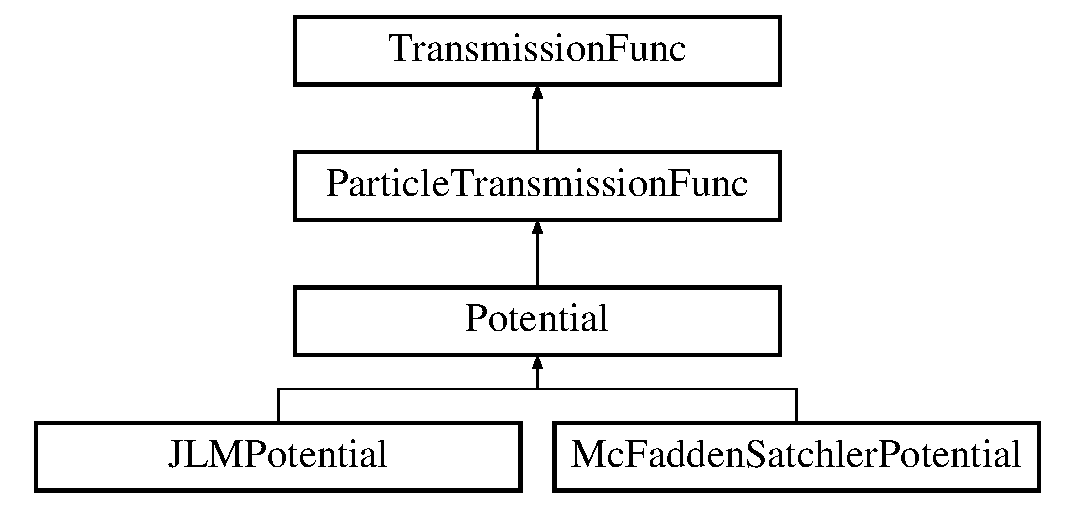
\includegraphics[height=4.000000cm]{dc/d66/classPotential}
\end{center}
\end{figure}
\subsection*{Public Member Functions}
\begin{DoxyCompactItemize}
\item 
\hyperlink{classPotential_a4fc0ce6be68500162a02df2175f6a122}{Potential} (int, int, int, int, double, int, double, int, double, int, double, double, double, double, \hyperlink{classTransmissionFunc}{Transmission\-Func} $\ast$)
\item 
\hyperlink{classPotential_ad50069dfb8df6538d94c4e3dcce26a6d}{$\sim$\-Potential} ()
\item 
int \hyperlink{classPotential_a0703b38c5987f1b81cbafae5a6d1ab0c}{Get\-Z1\-Z2} () const 
\item 
double \hyperlink{classPotential_a76d8dff6de0e098d8ec4fdf355363a57}{Get\-Boundary\-Radius} () const 
\item 
double \hyperlink{classPotential_a75d7cf1ca990cfe41be3e63caff7b2f1}{Get\-Red\-Mass} () const 
\item 
double \hyperlink{classPotential_a154fb8deeab61df6a0b55e2806844246}{Get\-R\-Max} () const 
\item 
virtual \hyperlink{Constants_8h_a1c1b16cc02d518bbe753449171ab7033}{std\-::complex}$<$ double $>$ \hyperlink{classPotential_af6d2217c4a1f91e7ebb84d5b728d11aa}{Calculate} (double, int, double, double, double) const =0
\item 
\hyperlink{Constants_8h_a1c1b16cc02d518bbe753449171ab7033}{std\-::complex}$<$ double $>$ \hyperlink{classPotential_a4e19e3b9ee8abf94d2c8e072daf46206}{Calc\-Beta} (double, int, double, double, double) const 
\item 
double \hyperlink{classPotential_aea8adb2a1783a79985621a899118c967}{Calc\-Transmission} (double, int, double)
\item 
void \hyperlink{classPotential_a6ecf02124b7690f05488a5fdde693d76}{Normalize\-Internally} (std\-::vector$<$ \hyperlink{Constants_8h_a1c1b16cc02d518bbe753449171ab7033}{std\-::complex}$<$ double $>$ $>$ \&, double) const 
\item 
void \hyperlink{classPotential_afaf287ffc13db37859773d092dcce2d9}{Normalize\-Over\-All\-Space} (std\-::vector$<$ \hyperlink{Constants_8h_a1c1b16cc02d518bbe753449171ab7033}{std\-::complex}$<$ double $>$ $>$ \&, double) const 
\item 
std\-::vector$<$ \hyperlink{Constants_8h_a1c1b16cc02d518bbe753449171ab7033}{std\-::complex}\\*
$<$ double $>$ $>$ \hyperlink{classPotential_a7af6c51bab5120e99024a73f79c84a37}{Solve} (double, int, double, double, double) const 
\end{DoxyCompactItemize}
\subsection*{Protected Attributes}
\begin{DoxyCompactItemize}
\item 
\hyperlink{classCoulFunc}{Coul\-Func} $\ast$ \hyperlink{classPotential_ab4d202d040f1b759ae2ce7ac6f0010e3}{coul\-Func\-\_\-}
\item 
double \hyperlink{classPotential_a0f692e07a6215ec4605ae1f04c09a926}{boundary\-Radius\-\_\-}
\item 
double \hyperlink{classPotential_a1ca2fe861ed14b351b2f884a6354ce90}{coulomb\-Radius\-\_\-}
\end{DoxyCompactItemize}
\subsection*{Additional Inherited Members}


\subsection{Constructor \& Destructor Documentation}
\hypertarget{classPotential_a4fc0ce6be68500162a02df2175f6a122}{\index{Potential@{Potential}!Potential@{Potential}}
\index{Potential@{Potential}!Potential@{Potential}}
\subsubsection[{Potential}]{\setlength{\rightskip}{0pt plus 5cm}Potential\-::\-Potential (
\begin{DoxyParamCaption}
\item[{int}]{z1, }
\item[{int}]{m1, }
\item[{int}]{z2, }
\item[{int}]{m2, }
\item[{double}]{j\-Initial, }
\item[{int}]{pi\-Initial, }
\item[{double}]{j\-Final, }
\item[{int}]{pi\-Final, }
\item[{double}]{spin, }
\item[{int}]{parity, }
\item[{double}]{max\-L, }
\item[{double}]{total\-Width\-For\-Correction, }
\item[{double}]{uncorr\-Total\-Width\-For\-Correction, }
\item[{double}]{uncorr\-Total\-Width\-Sqrd\-For\-Correction, }
\item[{{\bf Transmission\-Func} $\ast$}]{previous}
\end{DoxyParamCaption}
)}}\label{classPotential_a4fc0ce6be68500162a02df2175f6a122}


References coul\-Func\-\_\-, and Get\-Red\-Mass().

\hypertarget{classPotential_ad50069dfb8df6538d94c4e3dcce26a6d}{\index{Potential@{Potential}!$\sim$\-Potential@{$\sim$\-Potential}}
\index{$\sim$\-Potential@{$\sim$\-Potential}!Potential@{Potential}}
\subsubsection[{$\sim$\-Potential}]{\setlength{\rightskip}{0pt plus 5cm}Potential\-::$\sim$\-Potential (
\begin{DoxyParamCaption}
{}
\end{DoxyParamCaption}
)}}\label{classPotential_ad50069dfb8df6538d94c4e3dcce26a6d}


References coul\-Func\-\_\-.



\subsection{Member Function Documentation}
\hypertarget{classPotential_a4e19e3b9ee8abf94d2c8e072daf46206}{\index{Potential@{Potential}!Calc\-Beta@{Calc\-Beta}}
\index{Calc\-Beta@{Calc\-Beta}!Potential@{Potential}}
\subsubsection[{Calc\-Beta}]{\setlength{\rightskip}{0pt plus 5cm}{\bf std\-::complex}$<$ double $>$ Potential\-::\-Calc\-Beta (
\begin{DoxyParamCaption}
\item[{double}]{energy, }
\item[{int}]{l, }
\item[{double}]{s, }
\item[{double}]{j, }
\item[{double}]{r\-Step}
\end{DoxyParamCaption}
) const}}\label{classPotential_a4e19e3b9ee8abf94d2c8e072daf46206}


References Get\-Boundary\-Radius(), Normalize\-Internally(), and Solve().



Referenced by Calc\-Transmission().

\hypertarget{classPotential_aea8adb2a1783a79985621a899118c967}{\index{Potential@{Potential}!Calc\-Transmission@{Calc\-Transmission}}
\index{Calc\-Transmission@{Calc\-Transmission}!Potential@{Potential}}
\subsubsection[{Calc\-Transmission}]{\setlength{\rightskip}{0pt plus 5cm}double Potential\-::\-Calc\-Transmission (
\begin{DoxyParamCaption}
\item[{double}]{s, }
\item[{int}]{l, }
\item[{double}]{energy}
\end{DoxyParamCaption}
)\hspace{0.3cm}{\ttfamily [virtual]}}}\label{classPotential_aea8adb2a1783a79985621a899118c967}


Implements \hyperlink{classParticleTransmissionFunc_a651cc8a1d96d72e12eaf66506c046856}{Particle\-Transmission\-Func}.



References Calc\-Beta(), coul\-Func\-\_\-, Coul\-Waves\-::d\-F, Coul\-Waves\-::d\-G, Coul\-Waves\-::\-F, Coul\-Waves\-::\-G, Get\-Boundary\-Radius(), Get\-Red\-Mass(), hbarc, Transmission\-Func\-::j\-Initial\-\_\-, Particle\-Transmission\-Func\-::m1\-\_\-, and uconv.

\hypertarget{classPotential_af6d2217c4a1f91e7ebb84d5b728d11aa}{\index{Potential@{Potential}!Calculate@{Calculate}}
\index{Calculate@{Calculate}!Potential@{Potential}}
\subsubsection[{Calculate}]{\setlength{\rightskip}{0pt plus 5cm}virtual {\bf std\-::complex}$<$double$>$ Potential\-::\-Calculate (
\begin{DoxyParamCaption}
\item[{double}]{, }
\item[{int}]{, }
\item[{double}]{, }
\item[{double}]{, }
\item[{double}]{}
\end{DoxyParamCaption}
) const\hspace{0.3cm}{\ttfamily [pure virtual]}}}\label{classPotential_af6d2217c4a1f91e7ebb84d5b728d11aa}


Implemented in \hyperlink{classJLMPotential_ae9986807ce14a95a6c6214feea1233c8}{J\-L\-M\-Potential}, and \hyperlink{classMcFaddenSatchlerPotential_abbdff953b8577365fc0b60844d51ea4b}{Mc\-Fadden\-Satchler\-Potential}.



Referenced by Solve().

\hypertarget{classPotential_a76d8dff6de0e098d8ec4fdf355363a57}{\index{Potential@{Potential}!Get\-Boundary\-Radius@{Get\-Boundary\-Radius}}
\index{Get\-Boundary\-Radius@{Get\-Boundary\-Radius}!Potential@{Potential}}
\subsubsection[{Get\-Boundary\-Radius}]{\setlength{\rightskip}{0pt plus 5cm}double Potential\-::\-Get\-Boundary\-Radius (
\begin{DoxyParamCaption}
{}
\end{DoxyParamCaption}
) const\hspace{0.3cm}{\ttfamily [inline]}}}\label{classPotential_a76d8dff6de0e098d8ec4fdf355363a57}


References boundary\-Radius\-\_\-.



Referenced by Calc\-Beta(), Calc\-Transmission(), Normalize\-Internally(), and Solve().

\hypertarget{classPotential_a75d7cf1ca990cfe41be3e63caff7b2f1}{\index{Potential@{Potential}!Get\-Red\-Mass@{Get\-Red\-Mass}}
\index{Get\-Red\-Mass@{Get\-Red\-Mass}!Potential@{Potential}}
\subsubsection[{Get\-Red\-Mass}]{\setlength{\rightskip}{0pt plus 5cm}double Potential\-::\-Get\-Red\-Mass (
\begin{DoxyParamCaption}
{}
\end{DoxyParamCaption}
) const\hspace{0.3cm}{\ttfamily [inline]}}}\label{classPotential_a75d7cf1ca990cfe41be3e63caff7b2f1}


References Particle\-Transmission\-Func\-::redmass\-\_\-.



Referenced by Calc\-Transmission(), Potential(), and Solve().

\hypertarget{classPotential_a154fb8deeab61df6a0b55e2806844246}{\index{Potential@{Potential}!Get\-R\-Max@{Get\-R\-Max}}
\index{Get\-R\-Max@{Get\-R\-Max}!Potential@{Potential}}
\subsubsection[{Get\-R\-Max}]{\setlength{\rightskip}{0pt plus 5cm}double Potential\-::\-Get\-R\-Max (
\begin{DoxyParamCaption}
{}
\end{DoxyParamCaption}
) const\hspace{0.3cm}{\ttfamily [inline]}}}\label{classPotential_a154fb8deeab61df6a0b55e2806844246}


References boundary\-Radius\-\_\-.

\hypertarget{classPotential_a0703b38c5987f1b81cbafae5a6d1ab0c}{\index{Potential@{Potential}!Get\-Z1\-Z2@{Get\-Z1\-Z2}}
\index{Get\-Z1\-Z2@{Get\-Z1\-Z2}!Potential@{Potential}}
\subsubsection[{Get\-Z1\-Z2}]{\setlength{\rightskip}{0pt plus 5cm}int Potential\-::\-Get\-Z1\-Z2 (
\begin{DoxyParamCaption}
{}
\end{DoxyParamCaption}
) const\hspace{0.3cm}{\ttfamily [inline]}}}\label{classPotential_a0703b38c5987f1b81cbafae5a6d1ab0c}


References Particle\-Transmission\-Func\-::z1\-\_\-, and Transmission\-Func\-::z2\-\_\-.



Referenced by J\-L\-M\-Potential\-::\-Calculate(), and Mc\-Fadden\-Satchler\-Potential\-::\-Calculate().

\hypertarget{classPotential_a6ecf02124b7690f05488a5fdde693d76}{\index{Potential@{Potential}!Normalize\-Internally@{Normalize\-Internally}}
\index{Normalize\-Internally@{Normalize\-Internally}!Potential@{Potential}}
\subsubsection[{Normalize\-Internally}]{\setlength{\rightskip}{0pt plus 5cm}void Potential\-::\-Normalize\-Internally (
\begin{DoxyParamCaption}
\item[{std\-::vector$<$ {\bf std\-::complex}$<$ double $>$ $>$ \&}]{wave\-Function, }
\item[{double}]{r\-Step}
\end{DoxyParamCaption}
) const}}\label{classPotential_a6ecf02124b7690f05488a5fdde693d76}


References Get\-Boundary\-Radius().



Referenced by Calc\-Beta().

\hypertarget{classPotential_afaf287ffc13db37859773d092dcce2d9}{\index{Potential@{Potential}!Normalize\-Over\-All\-Space@{Normalize\-Over\-All\-Space}}
\index{Normalize\-Over\-All\-Space@{Normalize\-Over\-All\-Space}!Potential@{Potential}}
\subsubsection[{Normalize\-Over\-All\-Space}]{\setlength{\rightskip}{0pt plus 5cm}void Potential\-::\-Normalize\-Over\-All\-Space (
\begin{DoxyParamCaption}
\item[{std\-::vector$<$ {\bf std\-::complex}$<$ double $>$ $>$ \&}]{wave\-Function, }
\item[{double}]{r\-Step}
\end{DoxyParamCaption}
) const}}\label{classPotential_afaf287ffc13db37859773d092dcce2d9}
\hypertarget{classPotential_a7af6c51bab5120e99024a73f79c84a37}{\index{Potential@{Potential}!Solve@{Solve}}
\index{Solve@{Solve}!Potential@{Potential}}
\subsubsection[{Solve}]{\setlength{\rightskip}{0pt plus 5cm}std\-::vector$<$ {\bf std\-::complex}$<$ double $>$ $>$ Potential\-::\-Solve (
\begin{DoxyParamCaption}
\item[{double}]{energy, }
\item[{int}]{L, }
\item[{double}]{S, }
\item[{double}]{J, }
\item[{double}]{r\-Step}
\end{DoxyParamCaption}
) const}}\label{classPotential_a7af6c51bab5120e99024a73f79c84a37}


References Calculate(), Get\-Boundary\-Radius(), Get\-Red\-Mass(), hbarc, and uconv.



Referenced by Calc\-Beta().



\subsection{Member Data Documentation}
\hypertarget{classPotential_a0f692e07a6215ec4605ae1f04c09a926}{\index{Potential@{Potential}!boundary\-Radius\-\_\-@{boundary\-Radius\-\_\-}}
\index{boundary\-Radius\-\_\-@{boundary\-Radius\-\_\-}!Potential@{Potential}}
\subsubsection[{boundary\-Radius\-\_\-}]{\setlength{\rightskip}{0pt plus 5cm}double Potential\-::boundary\-Radius\-\_\-\hspace{0.3cm}{\ttfamily [protected]}}}\label{classPotential_a0f692e07a6215ec4605ae1f04c09a926}


Referenced by Get\-Boundary\-Radius(), Get\-R\-Max(), J\-L\-M\-Potential\-::\-J\-L\-M\-Potential(), and Mc\-Fadden\-Satchler\-Potential\-::\-Mc\-Fadden\-Satchler\-Potential().

\hypertarget{classPotential_ab4d202d040f1b759ae2ce7ac6f0010e3}{\index{Potential@{Potential}!coul\-Func\-\_\-@{coul\-Func\-\_\-}}
\index{coul\-Func\-\_\-@{coul\-Func\-\_\-}!Potential@{Potential}}
\subsubsection[{coul\-Func\-\_\-}]{\setlength{\rightskip}{0pt plus 5cm}{\bf Coul\-Func}$\ast$ Potential\-::coul\-Func\-\_\-\hspace{0.3cm}{\ttfamily [protected]}}}\label{classPotential_ab4d202d040f1b759ae2ce7ac6f0010e3}


Referenced by Calc\-Transmission(), Potential(), and $\sim$\-Potential().

\hypertarget{classPotential_a1ca2fe861ed14b351b2f884a6354ce90}{\index{Potential@{Potential}!coulomb\-Radius\-\_\-@{coulomb\-Radius\-\_\-}}
\index{coulomb\-Radius\-\_\-@{coulomb\-Radius\-\_\-}!Potential@{Potential}}
\subsubsection[{coulomb\-Radius\-\_\-}]{\setlength{\rightskip}{0pt plus 5cm}double Potential\-::coulomb\-Radius\-\_\-\hspace{0.3cm}{\ttfamily [protected]}}}\label{classPotential_a1ca2fe861ed14b351b2f884a6354ce90}


Referenced by J\-L\-M\-Potential\-::\-Calculate(), Mc\-Fadden\-Satchler\-Potential\-::\-Calculate(), J\-L\-M\-Potential\-::\-J\-L\-M\-Potential(), and Mc\-Fadden\-Satchler\-Potential\-::\-Mc\-Fadden\-Satchler\-Potential().



The documentation for this class was generated from the following files\-:\begin{DoxyCompactItemize}
\item 
/afs/crc.\-nd.\-edu/user/p/pscholz/\-Private/sapphire-\/devel/include/\hyperlink{Potential_8h}{Potential.\-h}\item 
/afs/crc.\-nd.\-edu/user/p/pscholz/\-Private/sapphire-\/devel/src/\hyperlink{Potential_8cpp}{Potential.\-cpp}\end{DoxyCompactItemize}

\hypertarget{classPreEqCDFEntry}{\section{Pre\-Eq\-C\-D\-F\-Entry Class Reference}
\label{classPreEqCDFEntry}\index{Pre\-Eq\-C\-D\-F\-Entry@{Pre\-Eq\-C\-D\-F\-Entry}}
}


{\ttfamily \#include $<$Pre\-Eq\-Decayer.\-h$>$}

\subsection*{Public Member Functions}
\begin{DoxyCompactItemize}
\item 
\hyperlink{classPreEqCDFEntry_ab6b57a5a386dadc860e58c1347beeccd}{Pre\-Eq\-C\-D\-F\-Entry} (int pair\-Index, double energy, double value)
\end{DoxyCompactItemize}
\subsection*{Public Attributes}
\begin{DoxyCompactItemize}
\item 
int \hyperlink{classPreEqCDFEntry_a26ae0cab9ef4a3cea18e5fcdd9a95219}{pair\-Index\-\_\-}
\item 
double \hyperlink{classPreEqCDFEntry_a59bcfcf73dfbcc3af62cdbd85b3299dc}{energy\-\_\-}
\item 
double \hyperlink{classPreEqCDFEntry_ab45f5e96c71a4f89a19bd9f0b4160fb8}{value\-\_\-}
\end{DoxyCompactItemize}


\subsection{Constructor \& Destructor Documentation}
\hypertarget{classPreEqCDFEntry_ab6b57a5a386dadc860e58c1347beeccd}{\index{Pre\-Eq\-C\-D\-F\-Entry@{Pre\-Eq\-C\-D\-F\-Entry}!Pre\-Eq\-C\-D\-F\-Entry@{Pre\-Eq\-C\-D\-F\-Entry}}
\index{Pre\-Eq\-C\-D\-F\-Entry@{Pre\-Eq\-C\-D\-F\-Entry}!PreEqCDFEntry@{Pre\-Eq\-C\-D\-F\-Entry}}
\subsubsection[{Pre\-Eq\-C\-D\-F\-Entry}]{\setlength{\rightskip}{0pt plus 5cm}Pre\-Eq\-C\-D\-F\-Entry\-::\-Pre\-Eq\-C\-D\-F\-Entry (
\begin{DoxyParamCaption}
\item[{int}]{pair\-Index, }
\item[{double}]{energy, }
\item[{double}]{value}
\end{DoxyParamCaption}
)\hspace{0.3cm}{\ttfamily [inline]}}}\label{classPreEqCDFEntry_ab6b57a5a386dadc860e58c1347beeccd}


\subsection{Member Data Documentation}
\hypertarget{classPreEqCDFEntry_a59bcfcf73dfbcc3af62cdbd85b3299dc}{\index{Pre\-Eq\-C\-D\-F\-Entry@{Pre\-Eq\-C\-D\-F\-Entry}!energy\-\_\-@{energy\-\_\-}}
\index{energy\-\_\-@{energy\-\_\-}!PreEqCDFEntry@{Pre\-Eq\-C\-D\-F\-Entry}}
\subsubsection[{energy\-\_\-}]{\setlength{\rightskip}{0pt plus 5cm}double Pre\-Eq\-C\-D\-F\-Entry\-::energy\-\_\-}}\label{classPreEqCDFEntry_a59bcfcf73dfbcc3af62cdbd85b3299dc}
\hypertarget{classPreEqCDFEntry_a26ae0cab9ef4a3cea18e5fcdd9a95219}{\index{Pre\-Eq\-C\-D\-F\-Entry@{Pre\-Eq\-C\-D\-F\-Entry}!pair\-Index\-\_\-@{pair\-Index\-\_\-}}
\index{pair\-Index\-\_\-@{pair\-Index\-\_\-}!PreEqCDFEntry@{Pre\-Eq\-C\-D\-F\-Entry}}
\subsubsection[{pair\-Index\-\_\-}]{\setlength{\rightskip}{0pt plus 5cm}int Pre\-Eq\-C\-D\-F\-Entry\-::pair\-Index\-\_\-}}\label{classPreEqCDFEntry_a26ae0cab9ef4a3cea18e5fcdd9a95219}
\hypertarget{classPreEqCDFEntry_ab45f5e96c71a4f89a19bd9f0b4160fb8}{\index{Pre\-Eq\-C\-D\-F\-Entry@{Pre\-Eq\-C\-D\-F\-Entry}!value\-\_\-@{value\-\_\-}}
\index{value\-\_\-@{value\-\_\-}!PreEqCDFEntry@{Pre\-Eq\-C\-D\-F\-Entry}}
\subsubsection[{value\-\_\-}]{\setlength{\rightskip}{0pt plus 5cm}double Pre\-Eq\-C\-D\-F\-Entry\-::value\-\_\-}}\label{classPreEqCDFEntry_ab45f5e96c71a4f89a19bd9f0b4160fb8}


The documentation for this class was generated from the following file\-:\begin{DoxyCompactItemize}
\item 
include/\hyperlink{PreEqDecayer_8h}{Pre\-Eq\-Decayer.\-h}\end{DoxyCompactItemize}

\hypertarget{classPreEqDecayer}{\section{Pre\-Eq\-Decayer Class Reference}
\label{classPreEqDecayer}\index{Pre\-Eq\-Decayer@{Pre\-Eq\-Decayer}}
}


{\ttfamily \#include $<$Pre\-Eq\-Decayer.\-h$>$}

\subsection*{Public Member Functions}
\begin{DoxyCompactItemize}
\item 
\hyperlink{classPreEqDecayer_a8eafff7cfc561e9de6e201d0efb4809f}{Pre\-Eq\-Decayer} (int initial\-Neutron\-Number, int initial\-Neutron\-Hole\-Number, int initial\-Proton\-Number, int initial\-Proton\-Hole\-Number, int Z, int A, double j\-Initial, int pi\-Initial, double energy)
\item 
\hyperlink{classPreEqDecayer_a7f7ab17d5c24d2977251d1977d782ba9}{$\sim$\-Pre\-Eq\-Decayer} ()
\item 
bool \hyperlink{classPreEqDecayer_a11702c60685b81a22d020fee52a70154}{Decay} (int \&, int \&, double \&, int \&, int \&, int \&, int \&, int \&, double \&, double \&)
\item 
void \hyperlink{classPreEqDecayer_ab10910a634239b5ce881b910049e0f2f}{Print\-C\-D\-F} ()
\end{DoxyCompactItemize}
\subsection*{Static Public Member Functions}
\begin{DoxyCompactItemize}
\item 
static void \hyperlink{classPreEqDecayer_ad03cef42114b546909988e4729ef2e0a}{Set\-Cross\-Section} (bool is\-Cross\-Section)
\item 
static void \hyperlink{classPreEqDecayer_ae113b36bfc5c46899d8ddaa6e1c4595a}{Set\-Max\-L} (double max\-L)
\item 
static double \hyperlink{classPreEqDecayer_a00e359b531369a0471b9c4dfc0b9ac6e}{Get\-Max\-L} ()
\end{DoxyCompactItemize}


\subsection{Constructor \& Destructor Documentation}
\hypertarget{classPreEqDecayer_a8eafff7cfc561e9de6e201d0efb4809f}{\index{Pre\-Eq\-Decayer@{Pre\-Eq\-Decayer}!Pre\-Eq\-Decayer@{Pre\-Eq\-Decayer}}
\index{Pre\-Eq\-Decayer@{Pre\-Eq\-Decayer}!PreEqDecayer@{Pre\-Eq\-Decayer}}
\subsubsection[{Pre\-Eq\-Decayer}]{\setlength{\rightskip}{0pt plus 5cm}Pre\-Eq\-Decayer\-::\-Pre\-Eq\-Decayer (
\begin{DoxyParamCaption}
\item[{int}]{initial\-Neutron\-Number, }
\item[{int}]{initial\-Neutron\-Hole\-Number, }
\item[{int}]{initial\-Proton\-Number, }
\item[{int}]{initial\-Proton\-Hole\-Number, }
\item[{int}]{Z, }
\item[{int}]{A, }
\item[{double}]{j\-Initial, }
\item[{int}]{pi\-Initial, }
\item[{double}]{energy}
\end{DoxyParamCaption}
)}}\label{classPreEqDecayer_a8eafff7cfc561e9de6e201d0efb4809f}


References Pre\-Eq\-Transition\-Rate\-Func\-::\-Integral(), and Nuclear\-Mass\-::\-Q\-Value().

\hypertarget{classPreEqDecayer_a7f7ab17d5c24d2977251d1977d782ba9}{\index{Pre\-Eq\-Decayer@{Pre\-Eq\-Decayer}!$\sim$\-Pre\-Eq\-Decayer@{$\sim$\-Pre\-Eq\-Decayer}}
\index{$\sim$\-Pre\-Eq\-Decayer@{$\sim$\-Pre\-Eq\-Decayer}!PreEqDecayer@{Pre\-Eq\-Decayer}}
\subsubsection[{$\sim$\-Pre\-Eq\-Decayer}]{\setlength{\rightskip}{0pt plus 5cm}Pre\-Eq\-Decayer\-::$\sim$\-Pre\-Eq\-Decayer (
\begin{DoxyParamCaption}
{}
\end{DoxyParamCaption}
)}}\label{classPreEqDecayer_a7f7ab17d5c24d2977251d1977d782ba9}


\subsection{Member Function Documentation}
\hypertarget{classPreEqDecayer_a11702c60685b81a22d020fee52a70154}{\index{Pre\-Eq\-Decayer@{Pre\-Eq\-Decayer}!Decay@{Decay}}
\index{Decay@{Decay}!PreEqDecayer@{Pre\-Eq\-Decayer}}
\subsubsection[{Decay}]{\setlength{\rightskip}{0pt plus 5cm}bool Pre\-Eq\-Decayer\-::\-Decay (
\begin{DoxyParamCaption}
\item[{int \&}]{Z, }
\item[{int \&}]{A, }
\item[{double \&}]{j\-Final, }
\item[{int \&}]{pi\-Final, }
\item[{int \&}]{neutron\-Number, }
\item[{int \&}]{neutron\-Hole\-Number, }
\item[{int \&}]{proton\-Number, }
\item[{int \&}]{proton\-Hole\-Number, }
\item[{double \&}]{excitation\-Energy, }
\item[{double \&}]{decay\-Energy}
\end{DoxyParamCaption}
)}}\label{classPreEqDecayer_a11702c60685b81a22d020fee52a70154}


References random\-Seed.



Referenced by Decay\-Controller\-::\-Decay().

\hypertarget{classPreEqDecayer_a00e359b531369a0471b9c4dfc0b9ac6e}{\index{Pre\-Eq\-Decayer@{Pre\-Eq\-Decayer}!Get\-Max\-L@{Get\-Max\-L}}
\index{Get\-Max\-L@{Get\-Max\-L}!PreEqDecayer@{Pre\-Eq\-Decayer}}
\subsubsection[{Get\-Max\-L}]{\setlength{\rightskip}{0pt plus 5cm}static double Pre\-Eq\-Decayer\-::\-Get\-Max\-L (
\begin{DoxyParamCaption}
{}
\end{DoxyParamCaption}
)\hspace{0.3cm}{\ttfamily [inline]}, {\ttfamily [static]}}}\label{classPreEqDecayer_a00e359b531369a0471b9c4dfc0b9ac6e}
\hypertarget{classPreEqDecayer_ab10910a634239b5ce881b910049e0f2f}{\index{Pre\-Eq\-Decayer@{Pre\-Eq\-Decayer}!Print\-C\-D\-F@{Print\-C\-D\-F}}
\index{Print\-C\-D\-F@{Print\-C\-D\-F}!PreEqDecayer@{Pre\-Eq\-Decayer}}
\subsubsection[{Print\-C\-D\-F}]{\setlength{\rightskip}{0pt plus 5cm}void Pre\-Eq\-Decayer\-::\-Print\-C\-D\-F (
\begin{DoxyParamCaption}
{}
\end{DoxyParamCaption}
)}}\label{classPreEqDecayer_ab10910a634239b5ce881b910049e0f2f}
\hypertarget{classPreEqDecayer_ad03cef42114b546909988e4729ef2e0a}{\index{Pre\-Eq\-Decayer@{Pre\-Eq\-Decayer}!Set\-Cross\-Section@{Set\-Cross\-Section}}
\index{Set\-Cross\-Section@{Set\-Cross\-Section}!PreEqDecayer@{Pre\-Eq\-Decayer}}
\subsubsection[{Set\-Cross\-Section}]{\setlength{\rightskip}{0pt plus 5cm}static void Pre\-Eq\-Decayer\-::\-Set\-Cross\-Section (
\begin{DoxyParamCaption}
\item[{bool}]{is\-Cross\-Section}
\end{DoxyParamCaption}
)\hspace{0.3cm}{\ttfamily [inline]}, {\ttfamily [static]}}}\label{classPreEqDecayer_ad03cef42114b546909988e4729ef2e0a}


Referenced by Initialize().

\hypertarget{classPreEqDecayer_ae113b36bfc5c46899d8ddaa6e1c4595a}{\index{Pre\-Eq\-Decayer@{Pre\-Eq\-Decayer}!Set\-Max\-L@{Set\-Max\-L}}
\index{Set\-Max\-L@{Set\-Max\-L}!PreEqDecayer@{Pre\-Eq\-Decayer}}
\subsubsection[{Set\-Max\-L}]{\setlength{\rightskip}{0pt plus 5cm}static void Pre\-Eq\-Decayer\-::\-Set\-Max\-L (
\begin{DoxyParamCaption}
\item[{double}]{max\-L}
\end{DoxyParamCaption}
)\hspace{0.3cm}{\ttfamily [inline]}, {\ttfamily [static]}}}\label{classPreEqDecayer_ae113b36bfc5c46899d8ddaa6e1c4595a}


Referenced by Initialize().



The documentation for this class was generated from the following files\-:\begin{DoxyCompactItemize}
\item 
include/\hyperlink{PreEqDecayer_8h}{Pre\-Eq\-Decayer.\-h}\item 
src/\hyperlink{PreEqDecayer_8cpp}{Pre\-Eq\-Decayer.\-cpp}\item 
src/\hyperlink{Setup_8cpp}{Setup.\-cpp}\end{DoxyCompactItemize}

\hypertarget{classPreEqSpinRatePair}{\section{Pre\-Eq\-Spin\-Rate\-Pair Class Reference}
\label{classPreEqSpinRatePair}\index{Pre\-Eq\-Spin\-Rate\-Pair@{Pre\-Eq\-Spin\-Rate\-Pair}}
}


{\ttfamily \#include $<$Pre\-Eq\-Decayer.\-h$>$}

\subsection*{Public Member Functions}
\begin{DoxyCompactItemize}
\item 
\hyperlink{classPreEqSpinRatePair_a143a6b3e33e768e4f596acbc6a55df3d}{Pre\-Eq\-Spin\-Rate\-Pair} (int neutron\-Number, int neutron\-Hole\-Number, int proton\-Number, int proton\-Hole\-Number, int Z, int A, double spin, int parity, double q\-Value, \hyperlink{classPreEqTransitionRateFunc}{Pre\-Eq\-Transition\-Rate\-Func} $\ast$rate\-Func, double integral)
\end{DoxyCompactItemize}
\subsection*{Public Attributes}
\begin{DoxyCompactItemize}
\item 
\hyperlink{classPreEqTransitionRateFunc}{Pre\-Eq\-Transition\-Rate\-Func} $\ast$ \hyperlink{classPreEqSpinRatePair_aeb84334cfe9778a95c2b45e99dc4eb43}{rate\-Func\-\_\-}
\item 
int \hyperlink{classPreEqSpinRatePair_a9b31793ff9418670b1ce4d1280414a18}{neutron\-Number\-\_\-}
\item 
int \hyperlink{classPreEqSpinRatePair_a3fca737c965ecbe7be4d8222ae3d6af5}{neutron\-Hole\-Number\-\_\-}
\item 
int \hyperlink{classPreEqSpinRatePair_a68a5d5e6475fc408f3617b65b1091e81}{proton\-Number\-\_\-}
\item 
int \hyperlink{classPreEqSpinRatePair_a22dee11a2b4677f2fd589619802adc5b}{proton\-Hole\-Number\-\_\-}
\item 
int \hyperlink{classPreEqSpinRatePair_afd6f7c07bd17e8fbdb7acabd763f2b92}{Z\-\_\-}
\item 
int \hyperlink{classPreEqSpinRatePair_af574e49be0ae28c28ea38c410b925a80}{A\-\_\-}
\item 
int \hyperlink{classPreEqSpinRatePair_a9901f86b3f463069aa0777e788f8292d}{parity\-\_\-}
\item 
double \hyperlink{classPreEqSpinRatePair_af88cd36daa52c5988fb000c0c67e49f9}{spin\-\_\-}
\item 
double \hyperlink{classPreEqSpinRatePair_a96304a72b8a4f972b98ed9149d6708f5}{q\-Value\-\_\-}
\item 
double \hyperlink{classPreEqSpinRatePair_a56396829690f3df1005a6bd025000286}{integral\-\_\-}
\end{DoxyCompactItemize}


\subsection{Constructor \& Destructor Documentation}
\hypertarget{classPreEqSpinRatePair_a143a6b3e33e768e4f596acbc6a55df3d}{\index{Pre\-Eq\-Spin\-Rate\-Pair@{Pre\-Eq\-Spin\-Rate\-Pair}!Pre\-Eq\-Spin\-Rate\-Pair@{Pre\-Eq\-Spin\-Rate\-Pair}}
\index{Pre\-Eq\-Spin\-Rate\-Pair@{Pre\-Eq\-Spin\-Rate\-Pair}!PreEqSpinRatePair@{Pre\-Eq\-Spin\-Rate\-Pair}}
\subsubsection[{Pre\-Eq\-Spin\-Rate\-Pair}]{\setlength{\rightskip}{0pt plus 5cm}Pre\-Eq\-Spin\-Rate\-Pair\-::\-Pre\-Eq\-Spin\-Rate\-Pair (
\begin{DoxyParamCaption}
\item[{int}]{neutron\-Number, }
\item[{int}]{neutron\-Hole\-Number, }
\item[{int}]{proton\-Number, }
\item[{int}]{proton\-Hole\-Number, }
\item[{int}]{Z, }
\item[{int}]{A, }
\item[{double}]{spin, }
\item[{int}]{parity, }
\item[{double}]{q\-Value, }
\item[{{\bf Pre\-Eq\-Transition\-Rate\-Func} $\ast$}]{rate\-Func, }
\item[{double}]{integral}
\end{DoxyParamCaption}
)\hspace{0.3cm}{\ttfamily [inline]}}}\label{classPreEqSpinRatePair_a143a6b3e33e768e4f596acbc6a55df3d}


\subsection{Member Data Documentation}
\hypertarget{classPreEqSpinRatePair_af574e49be0ae28c28ea38c410b925a80}{\index{Pre\-Eq\-Spin\-Rate\-Pair@{Pre\-Eq\-Spin\-Rate\-Pair}!A\-\_\-@{A\-\_\-}}
\index{A\-\_\-@{A\-\_\-}!PreEqSpinRatePair@{Pre\-Eq\-Spin\-Rate\-Pair}}
\subsubsection[{A\-\_\-}]{\setlength{\rightskip}{0pt plus 5cm}int Pre\-Eq\-Spin\-Rate\-Pair\-::\-A\-\_\-}}\label{classPreEqSpinRatePair_af574e49be0ae28c28ea38c410b925a80}
\hypertarget{classPreEqSpinRatePair_a56396829690f3df1005a6bd025000286}{\index{Pre\-Eq\-Spin\-Rate\-Pair@{Pre\-Eq\-Spin\-Rate\-Pair}!integral\-\_\-@{integral\-\_\-}}
\index{integral\-\_\-@{integral\-\_\-}!PreEqSpinRatePair@{Pre\-Eq\-Spin\-Rate\-Pair}}
\subsubsection[{integral\-\_\-}]{\setlength{\rightskip}{0pt plus 5cm}double Pre\-Eq\-Spin\-Rate\-Pair\-::integral\-\_\-}}\label{classPreEqSpinRatePair_a56396829690f3df1005a6bd025000286}
\hypertarget{classPreEqSpinRatePair_a3fca737c965ecbe7be4d8222ae3d6af5}{\index{Pre\-Eq\-Spin\-Rate\-Pair@{Pre\-Eq\-Spin\-Rate\-Pair}!neutron\-Hole\-Number\-\_\-@{neutron\-Hole\-Number\-\_\-}}
\index{neutron\-Hole\-Number\-\_\-@{neutron\-Hole\-Number\-\_\-}!PreEqSpinRatePair@{Pre\-Eq\-Spin\-Rate\-Pair}}
\subsubsection[{neutron\-Hole\-Number\-\_\-}]{\setlength{\rightskip}{0pt plus 5cm}int Pre\-Eq\-Spin\-Rate\-Pair\-::neutron\-Hole\-Number\-\_\-}}\label{classPreEqSpinRatePair_a3fca737c965ecbe7be4d8222ae3d6af5}
\hypertarget{classPreEqSpinRatePair_a9b31793ff9418670b1ce4d1280414a18}{\index{Pre\-Eq\-Spin\-Rate\-Pair@{Pre\-Eq\-Spin\-Rate\-Pair}!neutron\-Number\-\_\-@{neutron\-Number\-\_\-}}
\index{neutron\-Number\-\_\-@{neutron\-Number\-\_\-}!PreEqSpinRatePair@{Pre\-Eq\-Spin\-Rate\-Pair}}
\subsubsection[{neutron\-Number\-\_\-}]{\setlength{\rightskip}{0pt plus 5cm}int Pre\-Eq\-Spin\-Rate\-Pair\-::neutron\-Number\-\_\-}}\label{classPreEqSpinRatePair_a9b31793ff9418670b1ce4d1280414a18}
\hypertarget{classPreEqSpinRatePair_a9901f86b3f463069aa0777e788f8292d}{\index{Pre\-Eq\-Spin\-Rate\-Pair@{Pre\-Eq\-Spin\-Rate\-Pair}!parity\-\_\-@{parity\-\_\-}}
\index{parity\-\_\-@{parity\-\_\-}!PreEqSpinRatePair@{Pre\-Eq\-Spin\-Rate\-Pair}}
\subsubsection[{parity\-\_\-}]{\setlength{\rightskip}{0pt plus 5cm}int Pre\-Eq\-Spin\-Rate\-Pair\-::parity\-\_\-}}\label{classPreEqSpinRatePair_a9901f86b3f463069aa0777e788f8292d}
\hypertarget{classPreEqSpinRatePair_a22dee11a2b4677f2fd589619802adc5b}{\index{Pre\-Eq\-Spin\-Rate\-Pair@{Pre\-Eq\-Spin\-Rate\-Pair}!proton\-Hole\-Number\-\_\-@{proton\-Hole\-Number\-\_\-}}
\index{proton\-Hole\-Number\-\_\-@{proton\-Hole\-Number\-\_\-}!PreEqSpinRatePair@{Pre\-Eq\-Spin\-Rate\-Pair}}
\subsubsection[{proton\-Hole\-Number\-\_\-}]{\setlength{\rightskip}{0pt plus 5cm}int Pre\-Eq\-Spin\-Rate\-Pair\-::proton\-Hole\-Number\-\_\-}}\label{classPreEqSpinRatePair_a22dee11a2b4677f2fd589619802adc5b}
\hypertarget{classPreEqSpinRatePair_a68a5d5e6475fc408f3617b65b1091e81}{\index{Pre\-Eq\-Spin\-Rate\-Pair@{Pre\-Eq\-Spin\-Rate\-Pair}!proton\-Number\-\_\-@{proton\-Number\-\_\-}}
\index{proton\-Number\-\_\-@{proton\-Number\-\_\-}!PreEqSpinRatePair@{Pre\-Eq\-Spin\-Rate\-Pair}}
\subsubsection[{proton\-Number\-\_\-}]{\setlength{\rightskip}{0pt plus 5cm}int Pre\-Eq\-Spin\-Rate\-Pair\-::proton\-Number\-\_\-}}\label{classPreEqSpinRatePair_a68a5d5e6475fc408f3617b65b1091e81}
\hypertarget{classPreEqSpinRatePair_a96304a72b8a4f972b98ed9149d6708f5}{\index{Pre\-Eq\-Spin\-Rate\-Pair@{Pre\-Eq\-Spin\-Rate\-Pair}!q\-Value\-\_\-@{q\-Value\-\_\-}}
\index{q\-Value\-\_\-@{q\-Value\-\_\-}!PreEqSpinRatePair@{Pre\-Eq\-Spin\-Rate\-Pair}}
\subsubsection[{q\-Value\-\_\-}]{\setlength{\rightskip}{0pt plus 5cm}double Pre\-Eq\-Spin\-Rate\-Pair\-::q\-Value\-\_\-}}\label{classPreEqSpinRatePair_a96304a72b8a4f972b98ed9149d6708f5}
\hypertarget{classPreEqSpinRatePair_aeb84334cfe9778a95c2b45e99dc4eb43}{\index{Pre\-Eq\-Spin\-Rate\-Pair@{Pre\-Eq\-Spin\-Rate\-Pair}!rate\-Func\-\_\-@{rate\-Func\-\_\-}}
\index{rate\-Func\-\_\-@{rate\-Func\-\_\-}!PreEqSpinRatePair@{Pre\-Eq\-Spin\-Rate\-Pair}}
\subsubsection[{rate\-Func\-\_\-}]{\setlength{\rightskip}{0pt plus 5cm}{\bf Pre\-Eq\-Transition\-Rate\-Func}$\ast$ Pre\-Eq\-Spin\-Rate\-Pair\-::rate\-Func\-\_\-}}\label{classPreEqSpinRatePair_aeb84334cfe9778a95c2b45e99dc4eb43}
\hypertarget{classPreEqSpinRatePair_af88cd36daa52c5988fb000c0c67e49f9}{\index{Pre\-Eq\-Spin\-Rate\-Pair@{Pre\-Eq\-Spin\-Rate\-Pair}!spin\-\_\-@{spin\-\_\-}}
\index{spin\-\_\-@{spin\-\_\-}!PreEqSpinRatePair@{Pre\-Eq\-Spin\-Rate\-Pair}}
\subsubsection[{spin\-\_\-}]{\setlength{\rightskip}{0pt plus 5cm}double Pre\-Eq\-Spin\-Rate\-Pair\-::spin\-\_\-}}\label{classPreEqSpinRatePair_af88cd36daa52c5988fb000c0c67e49f9}
\hypertarget{classPreEqSpinRatePair_afd6f7c07bd17e8fbdb7acabd763f2b92}{\index{Pre\-Eq\-Spin\-Rate\-Pair@{Pre\-Eq\-Spin\-Rate\-Pair}!Z\-\_\-@{Z\-\_\-}}
\index{Z\-\_\-@{Z\-\_\-}!PreEqSpinRatePair@{Pre\-Eq\-Spin\-Rate\-Pair}}
\subsubsection[{Z\-\_\-}]{\setlength{\rightskip}{0pt plus 5cm}int Pre\-Eq\-Spin\-Rate\-Pair\-::\-Z\-\_\-}}\label{classPreEqSpinRatePair_afd6f7c07bd17e8fbdb7acabd763f2b92}


The documentation for this class was generated from the following file\-:\begin{DoxyCompactItemize}
\item 
include/\hyperlink{PreEqDecayer_8h}{Pre\-Eq\-Decayer.\-h}\end{DoxyCompactItemize}

\hypertarget{classPreEqTransitionRateFunc}{\section{Pre\-Eq\-Transition\-Rate\-Func Class Reference}
\label{classPreEqTransitionRateFunc}\index{Pre\-Eq\-Transition\-Rate\-Func@{Pre\-Eq\-Transition\-Rate\-Func}}
}


{\ttfamily \#include $<$Pre\-Eq\-Transition\-Rate\-Func.\-h$>$}

\subsection*{Public Member Functions}
\begin{DoxyCompactItemize}
\item 
\hyperlink{classPreEqTransitionRateFunc_a41e4aa6f4e9fa23fe5b3cef603de4e62}{Pre\-Eq\-Transition\-Rate\-Func} (int, int, int, int, int, int, int, int, int, int, int, int, double, int, double, int, double, int, double, double, double)
\item 
\hyperlink{classPreEqTransitionRateFunc_a3403caf6c009181e59bc1a942ceb45d4}{$\sim$\-Pre\-Eq\-Transition\-Rate\-Func} ()
\item 
double \hyperlink{classPreEqTransitionRateFunc_aad1a50ccd54be0f68a3f6181c59eb3f2}{Integral} () const 
\item 
std\-::vector$<$ \hyperlink{classXYPair}{X\-Y\-Pair} $>$ const \hyperlink{classPreEqTransitionRateFunc_ab509af190f43f46d28555535bd00737b}{Cumulative\-Sum} ()
\end{DoxyCompactItemize}


\subsection{Constructor \& Destructor Documentation}
\hypertarget{classPreEqTransitionRateFunc_a41e4aa6f4e9fa23fe5b3cef603de4e62}{\index{Pre\-Eq\-Transition\-Rate\-Func@{Pre\-Eq\-Transition\-Rate\-Func}!Pre\-Eq\-Transition\-Rate\-Func@{Pre\-Eq\-Transition\-Rate\-Func}}
\index{Pre\-Eq\-Transition\-Rate\-Func@{Pre\-Eq\-Transition\-Rate\-Func}!PreEqTransitionRateFunc@{Pre\-Eq\-Transition\-Rate\-Func}}
\subsubsection[{Pre\-Eq\-Transition\-Rate\-Func}]{\setlength{\rightskip}{0pt plus 5cm}Pre\-Eq\-Transition\-Rate\-Func\-::\-Pre\-Eq\-Transition\-Rate\-Func (
\begin{DoxyParamCaption}
\item[{int}]{z1, }
\item[{int}]{m1, }
\item[{int}]{z2, }
\item[{int}]{m2, }
\item[{int}]{initial\-Neutron\-Number, }
\item[{int}]{initial\-Neutron\-Hole\-Number, }
\item[{int}]{initial\-Proton\-Number, }
\item[{int}]{initial\-Proton\-Hole\-Number, }
\item[{int}]{final\-Neutron\-Number, }
\item[{int}]{final\-Neutron\-Hole\-Number, }
\item[{int}]{final\-Proton\-Number, }
\item[{int}]{final\-Proton\-Hole\-Number, }
\item[{double}]{j\-Initial, }
\item[{int}]{pi\-Initial, }
\item[{double}]{j\-Final, }
\item[{int}]{pi\-Final, }
\item[{double}]{spin, }
\item[{int}]{parity, }
\item[{double}]{max\-L, }
\item[{double}]{compound\-E, }
\item[{double}]{q\-Value}
\end{DoxyParamCaption}
)}}\label{classPreEqTransitionRateFunc_a41e4aa6f4e9fa23fe5b3cef603de4e62}
\hypertarget{classPreEqTransitionRateFunc_a3403caf6c009181e59bc1a942ceb45d4}{\index{Pre\-Eq\-Transition\-Rate\-Func@{Pre\-Eq\-Transition\-Rate\-Func}!$\sim$\-Pre\-Eq\-Transition\-Rate\-Func@{$\sim$\-Pre\-Eq\-Transition\-Rate\-Func}}
\index{$\sim$\-Pre\-Eq\-Transition\-Rate\-Func@{$\sim$\-Pre\-Eq\-Transition\-Rate\-Func}!PreEqTransitionRateFunc@{Pre\-Eq\-Transition\-Rate\-Func}}
\subsubsection[{$\sim$\-Pre\-Eq\-Transition\-Rate\-Func}]{\setlength{\rightskip}{0pt plus 5cm}Pre\-Eq\-Transition\-Rate\-Func\-::$\sim$\-Pre\-Eq\-Transition\-Rate\-Func (
\begin{DoxyParamCaption}
{}
\end{DoxyParamCaption}
)\hspace{0.3cm}{\ttfamily [inline]}}}\label{classPreEqTransitionRateFunc_a3403caf6c009181e59bc1a942ceb45d4}


\subsection{Member Function Documentation}
\hypertarget{classPreEqTransitionRateFunc_ab509af190f43f46d28555535bd00737b}{\index{Pre\-Eq\-Transition\-Rate\-Func@{Pre\-Eq\-Transition\-Rate\-Func}!Cumulative\-Sum@{Cumulative\-Sum}}
\index{Cumulative\-Sum@{Cumulative\-Sum}!PreEqTransitionRateFunc@{Pre\-Eq\-Transition\-Rate\-Func}}
\subsubsection[{Cumulative\-Sum}]{\setlength{\rightskip}{0pt plus 5cm}std\-::vector$<${\bf X\-Y\-Pair}$>$ const Pre\-Eq\-Transition\-Rate\-Func\-::\-Cumulative\-Sum (
\begin{DoxyParamCaption}
{}
\end{DoxyParamCaption}
)\hspace{0.3cm}{\ttfamily [inline]}}}\label{classPreEqTransitionRateFunc_ab509af190f43f46d28555535bd00737b}
\hypertarget{classPreEqTransitionRateFunc_aad1a50ccd54be0f68a3f6181c59eb3f2}{\index{Pre\-Eq\-Transition\-Rate\-Func@{Pre\-Eq\-Transition\-Rate\-Func}!Integral@{Integral}}
\index{Integral@{Integral}!PreEqTransitionRateFunc@{Pre\-Eq\-Transition\-Rate\-Func}}
\subsubsection[{Integral}]{\setlength{\rightskip}{0pt plus 5cm}double Pre\-Eq\-Transition\-Rate\-Func\-::\-Integral (
\begin{DoxyParamCaption}
{}
\end{DoxyParamCaption}
) const\hspace{0.3cm}{\ttfamily [inline]}}}\label{classPreEqTransitionRateFunc_aad1a50ccd54be0f68a3f6181c59eb3f2}


Referenced by Pre\-Eq\-Decayer\-::\-Pre\-Eq\-Decayer().



The documentation for this class was generated from the following files\-:\begin{DoxyCompactItemize}
\item 
/afs/crc.\-nd.\-edu/user/p/pscholz/\-Private/sapphire-\/devel/include/\hyperlink{PreEqTransitionRateFunc_8h}{Pre\-Eq\-Transition\-Rate\-Func.\-h}\item 
/afs/crc.\-nd.\-edu/user/p/pscholz/\-Private/sapphire-\/devel/src/\hyperlink{PreEqTransitionRateFunc_8cpp}{Pre\-Eq\-Transition\-Rate\-Func.\-cpp}\end{DoxyCompactItemize}

\hypertarget{classRauscherLevelDensity}{\section{Rauscher\-Level\-Density Class Reference}
\label{classRauscherLevelDensity}\index{Rauscher\-Level\-Density@{Rauscher\-Level\-Density}}
}


{\ttfamily \#include $<$Rauscher\-Level\-Density.\-h$>$}

Inheritance diagram for Rauscher\-Level\-Density\-:\begin{figure}[H]
\begin{center}
\leavevmode
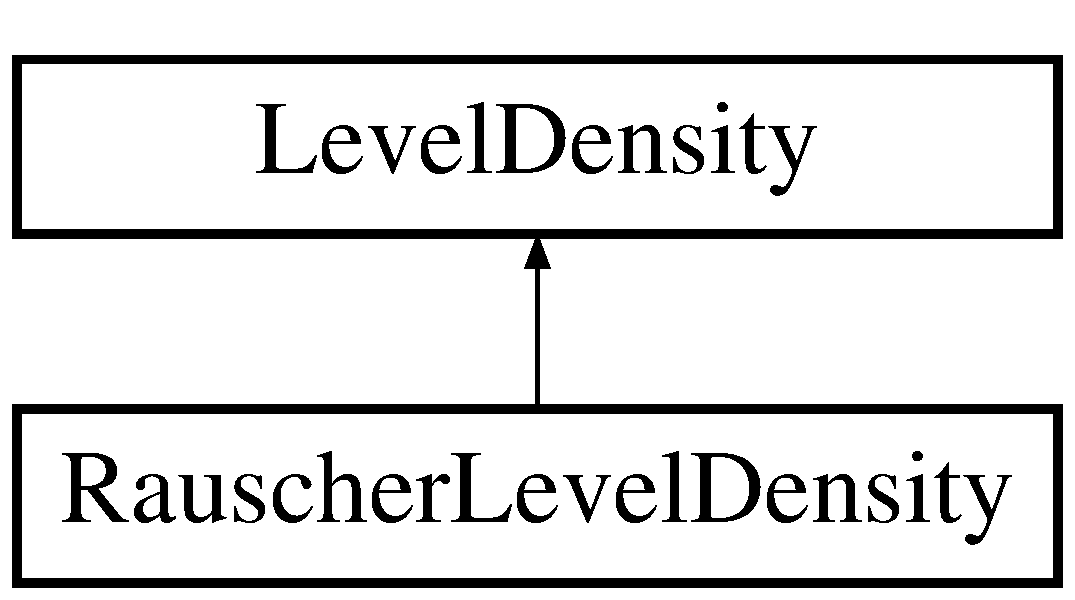
\includegraphics[height=2.000000cm]{dc/da8/classRauscherLevelDensity}
\end{center}
\end{figure}
\subsection*{Public Member Functions}
\begin{DoxyCompactItemize}
\item 
\hyperlink{classRauscherLevelDensity_a714feef52e449a86e2cf2ad23987a4a7}{Rauscher\-Level\-Density} (int Z, int A, double J)
\item 
\hyperlink{classRauscherLevelDensity_a796c7feb9d6c890d01b46f445238f9d6}{$\sim$\-Rauscher\-Level\-Density} ()
\item 
void \hyperlink{classRauscherLevelDensity_af5ce4f61ab69164ea0e8e47a4ed688c4}{Calc\-Back\-Shift} ()
\item 
double \hyperlink{classRauscherLevelDensity_a842444681f72b30d3dfbdf18ba95b207}{Calc\-Density\-Param} (double)
\item 
double \hyperlink{classRauscherLevelDensity_a734ed056ae869367c1cf295503c9d6aa}{Calc\-Nuclear\-Temp} (double)
\end{DoxyCompactItemize}
\subsection*{Additional Inherited Members}


\subsection{Constructor \& Destructor Documentation}
\hypertarget{classRauscherLevelDensity_a714feef52e449a86e2cf2ad23987a4a7}{\index{Rauscher\-Level\-Density@{Rauscher\-Level\-Density}!Rauscher\-Level\-Density@{Rauscher\-Level\-Density}}
\index{Rauscher\-Level\-Density@{Rauscher\-Level\-Density}!RauscherLevelDensity@{Rauscher\-Level\-Density}}
\subsubsection[{Rauscher\-Level\-Density}]{\setlength{\rightskip}{0pt plus 5cm}Rauscher\-Level\-Density\-::\-Rauscher\-Level\-Density (
\begin{DoxyParamCaption}
\item[{int}]{Z, }
\item[{int}]{A, }
\item[{double}]{J}
\end{DoxyParamCaption}
)\hspace{0.3cm}{\ttfamily [inline]}}}\label{classRauscherLevelDensity_a714feef52e449a86e2cf2ad23987a4a7}


References Calc\-Back\-Shift(), Level\-Density\-::\-Calc\-Constant\-Temp\-Terms(), and Nuclear\-Mass\-::\-Micro\-Energy\-Corr().

\hypertarget{classRauscherLevelDensity_a796c7feb9d6c890d01b46f445238f9d6}{\index{Rauscher\-Level\-Density@{Rauscher\-Level\-Density}!$\sim$\-Rauscher\-Level\-Density@{$\sim$\-Rauscher\-Level\-Density}}
\index{$\sim$\-Rauscher\-Level\-Density@{$\sim$\-Rauscher\-Level\-Density}!RauscherLevelDensity@{Rauscher\-Level\-Density}}
\subsubsection[{$\sim$\-Rauscher\-Level\-Density}]{\setlength{\rightskip}{0pt plus 5cm}Rauscher\-Level\-Density\-::$\sim$\-Rauscher\-Level\-Density (
\begin{DoxyParamCaption}
{}
\end{DoxyParamCaption}
)\hspace{0.3cm}{\ttfamily [inline]}}}\label{classRauscherLevelDensity_a796c7feb9d6c890d01b46f445238f9d6}


\subsection{Member Function Documentation}
\hypertarget{classRauscherLevelDensity_af5ce4f61ab69164ea0e8e47a4ed688c4}{\index{Rauscher\-Level\-Density@{Rauscher\-Level\-Density}!Calc\-Back\-Shift@{Calc\-Back\-Shift}}
\index{Calc\-Back\-Shift@{Calc\-Back\-Shift}!RauscherLevelDensity@{Rauscher\-Level\-Density}}
\subsubsection[{Calc\-Back\-Shift}]{\setlength{\rightskip}{0pt plus 5cm}void Rauscher\-Level\-Density\-::\-Calc\-Back\-Shift (
\begin{DoxyParamCaption}
{}
\end{DoxyParamCaption}
)\hspace{0.3cm}{\ttfamily [virtual]}}}\label{classRauscherLevelDensity_af5ce4f61ab69164ea0e8e47a4ed688c4}


Implements \hyperlink{classLevelDensity_a2aa1bbc8192a97c45be4f049dbd2dcc0}{Level\-Density}.



References Level\-Density\-::\-A\-\_\-, Level\-Density\-::backshift\-\_\-, Nuclear\-Mass\-::\-Neutron\-Pairing\-Gap(), Nuclear\-Mass\-::\-Proton\-Pairing\-Gap(), and Level\-Density\-::\-Z\-\_\-.



Referenced by Rauscher\-Level\-Density().

\hypertarget{classRauscherLevelDensity_a842444681f72b30d3dfbdf18ba95b207}{\index{Rauscher\-Level\-Density@{Rauscher\-Level\-Density}!Calc\-Density\-Param@{Calc\-Density\-Param}}
\index{Calc\-Density\-Param@{Calc\-Density\-Param}!RauscherLevelDensity@{Rauscher\-Level\-Density}}
\subsubsection[{Calc\-Density\-Param}]{\setlength{\rightskip}{0pt plus 5cm}double Rauscher\-Level\-Density\-::\-Calc\-Density\-Param (
\begin{DoxyParamCaption}
\item[{double}]{u}
\end{DoxyParamCaption}
)\hspace{0.3cm}{\ttfamily [virtual]}}}\label{classRauscherLevelDensity_a842444681f72b30d3dfbdf18ba95b207}


Implements \hyperlink{classLevelDensity_a42de1e15ee79bc984923b29b44ec55d5}{Level\-Density}.



Referenced by Calc\-Nuclear\-Temp().

\hypertarget{classRauscherLevelDensity_a734ed056ae869367c1cf295503c9d6aa}{\index{Rauscher\-Level\-Density@{Rauscher\-Level\-Density}!Calc\-Nuclear\-Temp@{Calc\-Nuclear\-Temp}}
\index{Calc\-Nuclear\-Temp@{Calc\-Nuclear\-Temp}!RauscherLevelDensity@{Rauscher\-Level\-Density}}
\subsubsection[{Calc\-Nuclear\-Temp}]{\setlength{\rightskip}{0pt plus 5cm}double Rauscher\-Level\-Density\-::\-Calc\-Nuclear\-Temp (
\begin{DoxyParamCaption}
\item[{double}]{u}
\end{DoxyParamCaption}
)\hspace{0.3cm}{\ttfamily [virtual]}}}\label{classRauscherLevelDensity_a734ed056ae869367c1cf295503c9d6aa}


Implements \hyperlink{classLevelDensity_a6a19c56e9784c0f1dac0ca2b86397c20}{Level\-Density}.



References Calc\-Density\-Param().



The documentation for this class was generated from the following files\-:\begin{DoxyCompactItemize}
\item 
include/\hyperlink{RauscherLevelDensity_8h}{Rauscher\-Level\-Density.\-h}\item 
src/\hyperlink{RauscherLevelDensity_8cpp}{Rauscher\-Level\-Density.\-cpp}\end{DoxyCompactItemize}

\hypertarget{classSLPair}{\section{S\-L\-Pair Class Reference}
\label{classSLPair}\index{S\-L\-Pair@{S\-L\-Pair}}
}


{\ttfamily \#include $<$Particle\-Transmission\-Func.\-h$>$}

\subsection*{Public Member Functions}
\begin{DoxyCompactItemize}
\item 
\hyperlink{classSLPair_a9f001d23e5d2408f9b4a76b24fc274f8}{S\-L\-Pair} (double s, int l)
\item 
bool \hyperlink{classSLPair_a5cf996af81044a6bdadc52ce8c7a033c}{operator$<$} (const \hyperlink{classSLPair}{S\-L\-Pair} \&right) const 
\end{DoxyCompactItemize}
\subsection*{Public Attributes}
\begin{DoxyCompactItemize}
\item 
double \hyperlink{classSLPair_abed67118ece6d1ed90508263fd4bb5e4}{s\-\_\-}
\item 
int \hyperlink{classSLPair_a50daebc25498be915489f00277f6f7b7}{l\-\_\-}
\end{DoxyCompactItemize}


\subsection{Constructor \& Destructor Documentation}
\hypertarget{classSLPair_a9f001d23e5d2408f9b4a76b24fc274f8}{\index{S\-L\-Pair@{S\-L\-Pair}!S\-L\-Pair@{S\-L\-Pair}}
\index{S\-L\-Pair@{S\-L\-Pair}!SLPair@{S\-L\-Pair}}
\subsubsection[{S\-L\-Pair}]{\setlength{\rightskip}{0pt plus 5cm}S\-L\-Pair\-::\-S\-L\-Pair (
\begin{DoxyParamCaption}
\item[{double}]{s, }
\item[{int}]{l}
\end{DoxyParamCaption}
)\hspace{0.3cm}{\ttfamily [inline]}}}\label{classSLPair_a9f001d23e5d2408f9b4a76b24fc274f8}


\subsection{Member Function Documentation}
\hypertarget{classSLPair_a5cf996af81044a6bdadc52ce8c7a033c}{\index{S\-L\-Pair@{S\-L\-Pair}!operator$<$@{operator$<$}}
\index{operator$<$@{operator$<$}!SLPair@{S\-L\-Pair}}
\subsubsection[{operator$<$}]{\setlength{\rightskip}{0pt plus 5cm}bool S\-L\-Pair\-::operator$<$ (
\begin{DoxyParamCaption}
\item[{const {\bf S\-L\-Pair} \&}]{right}
\end{DoxyParamCaption}
) const\hspace{0.3cm}{\ttfamily [inline]}}}\label{classSLPair_a5cf996af81044a6bdadc52ce8c7a033c}


References l\-\_\-, and s\-\_\-.



\subsection{Member Data Documentation}
\hypertarget{classSLPair_a50daebc25498be915489f00277f6f7b7}{\index{S\-L\-Pair@{S\-L\-Pair}!l\-\_\-@{l\-\_\-}}
\index{l\-\_\-@{l\-\_\-}!SLPair@{S\-L\-Pair}}
\subsubsection[{l\-\_\-}]{\setlength{\rightskip}{0pt plus 5cm}int S\-L\-Pair\-::l\-\_\-}}\label{classSLPair_a50daebc25498be915489f00277f6f7b7}


Referenced by operator$<$().

\hypertarget{classSLPair_abed67118ece6d1ed90508263fd4bb5e4}{\index{S\-L\-Pair@{S\-L\-Pair}!s\-\_\-@{s\-\_\-}}
\index{s\-\_\-@{s\-\_\-}!SLPair@{S\-L\-Pair}}
\subsubsection[{s\-\_\-}]{\setlength{\rightskip}{0pt plus 5cm}double S\-L\-Pair\-::s\-\_\-}}\label{classSLPair_abed67118ece6d1ed90508263fd4bb5e4}


Referenced by operator$<$().



The documentation for this class was generated from the following file\-:\begin{DoxyCompactItemize}
\item 
/afs/crc.\-nd.\-edu/user/p/pscholz/\-Private/sapphire-\/devel/include/\hyperlink{ParticleTransmissionFunc_8h}{Particle\-Transmission\-Func.\-h}\end{DoxyCompactItemize}

\hypertarget{classSpinRatePair}{\section{Spin\-Rate\-Pair Class Reference}
\label{classSpinRatePair}\index{Spin\-Rate\-Pair@{Spin\-Rate\-Pair}}
}


{\ttfamily \#include $<$Decayer.\-h$>$}

\subsection*{Public Member Functions}
\begin{DoxyCompactItemize}
\item 
\hyperlink{classSpinRatePair_a041ba492d89c65a3a08c8ab7043bd56e}{Spin\-Rate\-Pair} (int Z, int A, double spin, int parity, double q\-Value, \hyperlink{classTransitionRateFunc}{Transition\-Rate\-Func} $\ast$rate\-Func, double integral)
\end{DoxyCompactItemize}
\subsection*{Public Attributes}
\begin{DoxyCompactItemize}
\item 
\hyperlink{classTransitionRateFunc}{Transition\-Rate\-Func} $\ast$ \hyperlink{classSpinRatePair_a707563d58850763b4c67256ed3b36b6e}{rate\-Func\-\_\-}
\item 
int \hyperlink{classSpinRatePair_abcfea082d53a68d433b3deac710f1731}{Z\-\_\-}
\item 
int \hyperlink{classSpinRatePair_a84871c2c6b1c5e5e494bb613e78333e3}{A\-\_\-}
\item 
int \hyperlink{classSpinRatePair_af399ce33ae6123fa1ec7173932640533}{parity\-\_\-}
\item 
double \hyperlink{classSpinRatePair_ab52ca1bd083db60ceaf8fe58b4647669}{spin\-\_\-}
\item 
double \hyperlink{classSpinRatePair_af4ac45dc668f2bb9a01039f4a454d980}{q\-Value\-\_\-}
\item 
double \hyperlink{classSpinRatePair_a824af3ac72d5a9e35f12198dbe8ad182}{integral\-\_\-}
\end{DoxyCompactItemize}


\subsection{Constructor \& Destructor Documentation}
\hypertarget{classSpinRatePair_a041ba492d89c65a3a08c8ab7043bd56e}{\index{Spin\-Rate\-Pair@{Spin\-Rate\-Pair}!Spin\-Rate\-Pair@{Spin\-Rate\-Pair}}
\index{Spin\-Rate\-Pair@{Spin\-Rate\-Pair}!SpinRatePair@{Spin\-Rate\-Pair}}
\subsubsection[{Spin\-Rate\-Pair}]{\setlength{\rightskip}{0pt plus 5cm}Spin\-Rate\-Pair\-::\-Spin\-Rate\-Pair (
\begin{DoxyParamCaption}
\item[{int}]{Z, }
\item[{int}]{A, }
\item[{double}]{spin, }
\item[{int}]{parity, }
\item[{double}]{q\-Value, }
\item[{{\bf Transition\-Rate\-Func} $\ast$}]{rate\-Func, }
\item[{double}]{integral}
\end{DoxyParamCaption}
)\hspace{0.3cm}{\ttfamily [inline]}}}\label{classSpinRatePair_a041ba492d89c65a3a08c8ab7043bd56e}


\subsection{Member Data Documentation}
\hypertarget{classSpinRatePair_a84871c2c6b1c5e5e494bb613e78333e3}{\index{Spin\-Rate\-Pair@{Spin\-Rate\-Pair}!A\-\_\-@{A\-\_\-}}
\index{A\-\_\-@{A\-\_\-}!SpinRatePair@{Spin\-Rate\-Pair}}
\subsubsection[{A\-\_\-}]{\setlength{\rightskip}{0pt plus 5cm}int Spin\-Rate\-Pair\-::\-A\-\_\-}}\label{classSpinRatePair_a84871c2c6b1c5e5e494bb613e78333e3}
\hypertarget{classSpinRatePair_a824af3ac72d5a9e35f12198dbe8ad182}{\index{Spin\-Rate\-Pair@{Spin\-Rate\-Pair}!integral\-\_\-@{integral\-\_\-}}
\index{integral\-\_\-@{integral\-\_\-}!SpinRatePair@{Spin\-Rate\-Pair}}
\subsubsection[{integral\-\_\-}]{\setlength{\rightskip}{0pt plus 5cm}double Spin\-Rate\-Pair\-::integral\-\_\-}}\label{classSpinRatePair_a824af3ac72d5a9e35f12198dbe8ad182}
\hypertarget{classSpinRatePair_af399ce33ae6123fa1ec7173932640533}{\index{Spin\-Rate\-Pair@{Spin\-Rate\-Pair}!parity\-\_\-@{parity\-\_\-}}
\index{parity\-\_\-@{parity\-\_\-}!SpinRatePair@{Spin\-Rate\-Pair}}
\subsubsection[{parity\-\_\-}]{\setlength{\rightskip}{0pt plus 5cm}int Spin\-Rate\-Pair\-::parity\-\_\-}}\label{classSpinRatePair_af399ce33ae6123fa1ec7173932640533}
\hypertarget{classSpinRatePair_af4ac45dc668f2bb9a01039f4a454d980}{\index{Spin\-Rate\-Pair@{Spin\-Rate\-Pair}!q\-Value\-\_\-@{q\-Value\-\_\-}}
\index{q\-Value\-\_\-@{q\-Value\-\_\-}!SpinRatePair@{Spin\-Rate\-Pair}}
\subsubsection[{q\-Value\-\_\-}]{\setlength{\rightskip}{0pt plus 5cm}double Spin\-Rate\-Pair\-::q\-Value\-\_\-}}\label{classSpinRatePair_af4ac45dc668f2bb9a01039f4a454d980}
\hypertarget{classSpinRatePair_a707563d58850763b4c67256ed3b36b6e}{\index{Spin\-Rate\-Pair@{Spin\-Rate\-Pair}!rate\-Func\-\_\-@{rate\-Func\-\_\-}}
\index{rate\-Func\-\_\-@{rate\-Func\-\_\-}!SpinRatePair@{Spin\-Rate\-Pair}}
\subsubsection[{rate\-Func\-\_\-}]{\setlength{\rightskip}{0pt plus 5cm}{\bf Transition\-Rate\-Func}$\ast$ Spin\-Rate\-Pair\-::rate\-Func\-\_\-}}\label{classSpinRatePair_a707563d58850763b4c67256ed3b36b6e}
\hypertarget{classSpinRatePair_ab52ca1bd083db60ceaf8fe58b4647669}{\index{Spin\-Rate\-Pair@{Spin\-Rate\-Pair}!spin\-\_\-@{spin\-\_\-}}
\index{spin\-\_\-@{spin\-\_\-}!SpinRatePair@{Spin\-Rate\-Pair}}
\subsubsection[{spin\-\_\-}]{\setlength{\rightskip}{0pt plus 5cm}double Spin\-Rate\-Pair\-::spin\-\_\-}}\label{classSpinRatePair_ab52ca1bd083db60ceaf8fe58b4647669}
\hypertarget{classSpinRatePair_abcfea082d53a68d433b3deac710f1731}{\index{Spin\-Rate\-Pair@{Spin\-Rate\-Pair}!Z\-\_\-@{Z\-\_\-}}
\index{Z\-\_\-@{Z\-\_\-}!SpinRatePair@{Spin\-Rate\-Pair}}
\subsubsection[{Z\-\_\-}]{\setlength{\rightskip}{0pt plus 5cm}int Spin\-Rate\-Pair\-::\-Z\-\_\-}}\label{classSpinRatePair_abcfea082d53a68d433b3deac710f1731}


The documentation for this class was generated from the following file\-:\begin{DoxyCompactItemize}
\item 
/afs/crc.\-nd.\-edu/user/p/pscholz/\-Private/sapphire-\/devel/include/\hyperlink{Decayer_8h}{Decayer.\-h}\end{DoxyCompactItemize}

\hypertarget{classTransitionRateFunc}{\section{Transition\-Rate\-Func Class Reference}
\label{classTransitionRateFunc}\index{Transition\-Rate\-Func@{Transition\-Rate\-Func}}
}


{\ttfamily \#include $<$Transition\-Rate\-Func.\-h$>$}

\subsection*{Public Member Functions}
\begin{DoxyCompactItemize}
\item 
\hyperlink{classTransitionRateFunc_a358f40612d3c99b3891ea6b12986e731}{Transition\-Rate\-Func} (int, int, int, int, double, int, double, int, double, int, double, double, double, double, double, double, \hyperlink{classTransitionRateFunc}{Transition\-Rate\-Func} $\ast$, bool)
\item 
\hyperlink{classTransitionRateFunc_a8984bc603b33b245fe2a5a5329a3f67e}{$\sim$\-Transition\-Rate\-Func} ()
\item 
std\-::vector$<$ \hyperlink{classXYPair}{X\-Y\-Pair} $>$ const \hyperlink{classTransitionRateFunc_a4b9a309e9288c531912f9a2b424b6826}{Function} ()
\item 
std\-::vector$<$ \hyperlink{classXYPair}{X\-Y\-Pair} $>$ const \hyperlink{classTransitionRateFunc_a8403001845549cae39aa5c344fd97838}{Cumulative\-Sum} ()
\item 
double \hyperlink{classTransitionRateFunc_ac2e8e5c86c01bf2f0198d4c50c9272f9}{Integral} () const 
\item 
double \hyperlink{classTransitionRateFunc_a2131d16208035803f34bbf966d995fe1}{Calc\-Level\-Density} (double energy)
\item 
double \hyperlink{classTransitionRateFunc_acea0c4d2dbfe1a31bfb4ea5d2720e6b4}{Calc\-Transmission\-Func} (double energy)
\item 
double \hyperlink{classTransitionRateFunc_a03d1a328b3183d2eadb48d05b9d63597}{Calc\-Total\-Level\-Density} (double energy)
\item 
double \hyperlink{classTransitionRateFunc_aa75253d5839cd84ab00bdceaf8ca2e9d}{Exclusive\-Branching} () const 
\item 
double \hyperlink{classTransitionRateFunc_a9632cdbf1551e2b52cc7af595e1e3b65}{Ground\-State\-Transmission} () const 
\end{DoxyCompactItemize}
\subsection*{Static Public Member Functions}
\begin{DoxyCompactItemize}
\item 
static void \hyperlink{classTransitionRateFunc_a4f7aa579014a37666c5d6d3f2e71e07e}{Set\-Gamma\-Cutoff\-Energy} (double energy)
\item 
static double \hyperlink{classTransitionRateFunc_a15ef8d7f5a3a5e20046d5e11075b7e1f}{Get\-Gamma\-Cutoff\-Energy} ()
\end{DoxyCompactItemize}


\subsection{Constructor \& Destructor Documentation}
\hypertarget{classTransitionRateFunc_a358f40612d3c99b3891ea6b12986e731}{\index{Transition\-Rate\-Func@{Transition\-Rate\-Func}!Transition\-Rate\-Func@{Transition\-Rate\-Func}}
\index{Transition\-Rate\-Func@{Transition\-Rate\-Func}!TransitionRateFunc@{Transition\-Rate\-Func}}
\subsubsection[{Transition\-Rate\-Func}]{\setlength{\rightskip}{0pt plus 5cm}Transition\-Rate\-Func\-::\-Transition\-Rate\-Func (
\begin{DoxyParamCaption}
\item[{int}]{z1, }
\item[{int}]{m1, }
\item[{int}]{z2, }
\item[{int}]{m2, }
\item[{double}]{j\-Initial, }
\item[{int}]{pi\-Initial, }
\item[{double}]{j\-Final, }
\item[{int}]{pi\-Final, }
\item[{double}]{spin, }
\item[{int}]{parity, }
\item[{double}]{max\-L, }
\item[{double}]{compound\-E, }
\item[{double}]{q\-Value, }
\item[{double}]{total\-Width\-For\-Correction, }
\item[{double}]{uncorr\-Total\-Width\-For\-Correction, }
\item[{double}]{uncorr\-Total\-Width\-Sqrd\-For\-Correction, }
\item[{{\bf Transition\-Rate\-Func} $\ast$}]{previous, }
\item[{bool}]{is\-Cross\-Section}
\end{DoxyParamCaption}
)}}\label{classTransitionRateFunc_a358f40612d3c99b3891ea6b12986e731}


References Calc\-Level\-Density(), Calc\-Transmission\-Func(), Gamma\-Transmission\-Func\-::\-Create\-Gamma\-Transmission\-Func(), Particle\-Transmission\-Func\-::\-Create\-Particle\-Transmission\-Func(), Nuclear\-Levels\-::\-Find\-Levels(), Nuclear\-Mass\-::\-Highest\-Bound\-Energy(), and Transmission\-Func\-::\-Is\-Valid().

\hypertarget{classTransitionRateFunc_a8984bc603b33b245fe2a5a5329a3f67e}{\index{Transition\-Rate\-Func@{Transition\-Rate\-Func}!$\sim$\-Transition\-Rate\-Func@{$\sim$\-Transition\-Rate\-Func}}
\index{$\sim$\-Transition\-Rate\-Func@{$\sim$\-Transition\-Rate\-Func}!TransitionRateFunc@{Transition\-Rate\-Func}}
\subsubsection[{$\sim$\-Transition\-Rate\-Func}]{\setlength{\rightskip}{0pt plus 5cm}Transition\-Rate\-Func\-::$\sim$\-Transition\-Rate\-Func (
\begin{DoxyParamCaption}
{}
\end{DoxyParamCaption}
)\hspace{0.3cm}{\ttfamily [inline]}}}\label{classTransitionRateFunc_a8984bc603b33b245fe2a5a5329a3f67e}


\subsection{Member Function Documentation}
\hypertarget{classTransitionRateFunc_a2131d16208035803f34bbf966d995fe1}{\index{Transition\-Rate\-Func@{Transition\-Rate\-Func}!Calc\-Level\-Density@{Calc\-Level\-Density}}
\index{Calc\-Level\-Density@{Calc\-Level\-Density}!TransitionRateFunc@{Transition\-Rate\-Func}}
\subsubsection[{Calc\-Level\-Density}]{\setlength{\rightskip}{0pt plus 5cm}double Transition\-Rate\-Func\-::\-Calc\-Level\-Density (
\begin{DoxyParamCaption}
\item[{double}]{energy}
\end{DoxyParamCaption}
)\hspace{0.3cm}{\ttfamily [inline]}}}\label{classTransitionRateFunc_a2131d16208035803f34bbf966d995fe1}


Referenced by Transition\-Rate\-Func().

\hypertarget{classTransitionRateFunc_a03d1a328b3183d2eadb48d05b9d63597}{\index{Transition\-Rate\-Func@{Transition\-Rate\-Func}!Calc\-Total\-Level\-Density@{Calc\-Total\-Level\-Density}}
\index{Calc\-Total\-Level\-Density@{Calc\-Total\-Level\-Density}!TransitionRateFunc@{Transition\-Rate\-Func}}
\subsubsection[{Calc\-Total\-Level\-Density}]{\setlength{\rightskip}{0pt plus 5cm}double Transition\-Rate\-Func\-::\-Calc\-Total\-Level\-Density (
\begin{DoxyParamCaption}
\item[{double}]{energy}
\end{DoxyParamCaption}
)\hspace{0.3cm}{\ttfamily [inline]}}}\label{classTransitionRateFunc_a03d1a328b3183d2eadb48d05b9d63597}


References Level\-Density\-::\-Total\-Level\-Density().

\hypertarget{classTransitionRateFunc_acea0c4d2dbfe1a31bfb4ea5d2720e6b4}{\index{Transition\-Rate\-Func@{Transition\-Rate\-Func}!Calc\-Transmission\-Func@{Calc\-Transmission\-Func}}
\index{Calc\-Transmission\-Func@{Calc\-Transmission\-Func}!TransitionRateFunc@{Transition\-Rate\-Func}}
\subsubsection[{Calc\-Transmission\-Func}]{\setlength{\rightskip}{0pt plus 5cm}double Transition\-Rate\-Func\-::\-Calc\-Transmission\-Func (
\begin{DoxyParamCaption}
\item[{double}]{energy}
\end{DoxyParamCaption}
)\hspace{0.3cm}{\ttfamily [inline]}}}\label{classTransitionRateFunc_acea0c4d2dbfe1a31bfb4ea5d2720e6b4}


Referenced by Transition\-Rate\-Func().

\hypertarget{classTransitionRateFunc_a8403001845549cae39aa5c344fd97838}{\index{Transition\-Rate\-Func@{Transition\-Rate\-Func}!Cumulative\-Sum@{Cumulative\-Sum}}
\index{Cumulative\-Sum@{Cumulative\-Sum}!TransitionRateFunc@{Transition\-Rate\-Func}}
\subsubsection[{Cumulative\-Sum}]{\setlength{\rightskip}{0pt plus 5cm}std\-::vector$<${\bf X\-Y\-Pair}$>$ const Transition\-Rate\-Func\-::\-Cumulative\-Sum (
\begin{DoxyParamCaption}
{}
\end{DoxyParamCaption}
)\hspace{0.3cm}{\ttfamily [inline]}}}\label{classTransitionRateFunc_a8403001845549cae39aa5c344fd97838}
\hypertarget{classTransitionRateFunc_aa75253d5839cd84ab00bdceaf8ca2e9d}{\index{Transition\-Rate\-Func@{Transition\-Rate\-Func}!Exclusive\-Branching@{Exclusive\-Branching}}
\index{Exclusive\-Branching@{Exclusive\-Branching}!TransitionRateFunc@{Transition\-Rate\-Func}}
\subsubsection[{Exclusive\-Branching}]{\setlength{\rightskip}{0pt plus 5cm}double Transition\-Rate\-Func\-::\-Exclusive\-Branching (
\begin{DoxyParamCaption}
{}
\end{DoxyParamCaption}
) const\hspace{0.3cm}{\ttfamily [inline]}}}\label{classTransitionRateFunc_aa75253d5839cd84ab00bdceaf8ca2e9d}
\hypertarget{classTransitionRateFunc_a4b9a309e9288c531912f9a2b424b6826}{\index{Transition\-Rate\-Func@{Transition\-Rate\-Func}!Function@{Function}}
\index{Function@{Function}!TransitionRateFunc@{Transition\-Rate\-Func}}
\subsubsection[{Function}]{\setlength{\rightskip}{0pt plus 5cm}std\-::vector$<${\bf X\-Y\-Pair}$>$ const Transition\-Rate\-Func\-::\-Function (
\begin{DoxyParamCaption}
{}
\end{DoxyParamCaption}
)\hspace{0.3cm}{\ttfamily [inline]}}}\label{classTransitionRateFunc_a4b9a309e9288c531912f9a2b424b6826}
\hypertarget{classTransitionRateFunc_a15ef8d7f5a3a5e20046d5e11075b7e1f}{\index{Transition\-Rate\-Func@{Transition\-Rate\-Func}!Get\-Gamma\-Cutoff\-Energy@{Get\-Gamma\-Cutoff\-Energy}}
\index{Get\-Gamma\-Cutoff\-Energy@{Get\-Gamma\-Cutoff\-Energy}!TransitionRateFunc@{Transition\-Rate\-Func}}
\subsubsection[{Get\-Gamma\-Cutoff\-Energy}]{\setlength{\rightskip}{0pt plus 5cm}static double Transition\-Rate\-Func\-::\-Get\-Gamma\-Cutoff\-Energy (
\begin{DoxyParamCaption}
{}
\end{DoxyParamCaption}
)\hspace{0.3cm}{\ttfamily [inline]}, {\ttfamily [static]}}}\label{classTransitionRateFunc_a15ef8d7f5a3a5e20046d5e11075b7e1f}


Referenced by parse\-Command\-Line\-For\-Options().

\hypertarget{classTransitionRateFunc_a9632cdbf1551e2b52cc7af595e1e3b65}{\index{Transition\-Rate\-Func@{Transition\-Rate\-Func}!Ground\-State\-Transmission@{Ground\-State\-Transmission}}
\index{Ground\-State\-Transmission@{Ground\-State\-Transmission}!TransitionRateFunc@{Transition\-Rate\-Func}}
\subsubsection[{Ground\-State\-Transmission}]{\setlength{\rightskip}{0pt plus 5cm}double Transition\-Rate\-Func\-::\-Ground\-State\-Transmission (
\begin{DoxyParamCaption}
{}
\end{DoxyParamCaption}
) const\hspace{0.3cm}{\ttfamily [inline]}}}\label{classTransitionRateFunc_a9632cdbf1551e2b52cc7af595e1e3b65}


Referenced by Decayer\-::\-Decayer().

\hypertarget{classTransitionRateFunc_ac2e8e5c86c01bf2f0198d4c50c9272f9}{\index{Transition\-Rate\-Func@{Transition\-Rate\-Func}!Integral@{Integral}}
\index{Integral@{Integral}!TransitionRateFunc@{Transition\-Rate\-Func}}
\subsubsection[{Integral}]{\setlength{\rightskip}{0pt plus 5cm}double Transition\-Rate\-Func\-::\-Integral (
\begin{DoxyParamCaption}
{}
\end{DoxyParamCaption}
) const\hspace{0.3cm}{\ttfamily [inline]}}}\label{classTransitionRateFunc_ac2e8e5c86c01bf2f0198d4c50c9272f9}


Referenced by Decayer\-::\-Decayer().

\hypertarget{classTransitionRateFunc_a4f7aa579014a37666c5d6d3f2e71e07e}{\index{Transition\-Rate\-Func@{Transition\-Rate\-Func}!Set\-Gamma\-Cutoff\-Energy@{Set\-Gamma\-Cutoff\-Energy}}
\index{Set\-Gamma\-Cutoff\-Energy@{Set\-Gamma\-Cutoff\-Energy}!TransitionRateFunc@{Transition\-Rate\-Func}}
\subsubsection[{Set\-Gamma\-Cutoff\-Energy}]{\setlength{\rightskip}{0pt plus 5cm}static void Transition\-Rate\-Func\-::\-Set\-Gamma\-Cutoff\-Energy (
\begin{DoxyParamCaption}
\item[{double}]{energy}
\end{DoxyParamCaption}
)\hspace{0.3cm}{\ttfamily [inline]}, {\ttfamily [static]}}}\label{classTransitionRateFunc_a4f7aa579014a37666c5d6d3f2e71e07e}


Referenced by Cross\-Section\-::\-Calculate(), Initialize(), and parse\-Command\-Line\-For\-Options().



The documentation for this class was generated from the following files\-:\begin{DoxyCompactItemize}
\item 
include/\hyperlink{TransitionRateFunc_8h}{Transition\-Rate\-Func.\-h}\item 
src/\hyperlink{Setup_8cpp}{Setup.\-cpp}\item 
src/\hyperlink{TransitionRateFunc_8cpp}{Transition\-Rate\-Func.\-cpp}\end{DoxyCompactItemize}

\hypertarget{classTransmissionFunc}{\section{Transmission\-Func Class Reference}
\label{classTransmissionFunc}\index{Transmission\-Func@{Transmission\-Func}}
}


{\ttfamily \#include $<$Transmission\-Func.\-h$>$}

Inheritance diagram for Transmission\-Func\-:\begin{figure}[H]
\begin{center}
\leavevmode
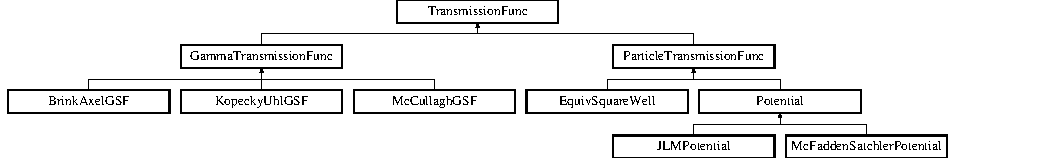
\includegraphics[height=2.121212cm]{dc/d0d/classTransmissionFunc}
\end{center}
\end{figure}
\subsection*{Public Member Functions}
\begin{DoxyCompactItemize}
\item 
\hyperlink{classTransmissionFunc_a6c7c0f1a3c272a9942e897328747ccce}{Transmission\-Func} (int z2, int m2, double j\-Initial, int pi\-Initial, double j\-Final, int pi\-Final, double max\-L, double total\-Width\-For\-Correction, double uncorr\-Total\-Width\-For\-Correction, double uncorr\-Total\-Width\-Sqrd\-For\-Correction, \hyperlink{classTransmissionFunc}{Transmission\-Func} $\ast$previous)
\item 
virtual \hyperlink{classTransmissionFunc_a8f3c3437541f0cb96a6cef9a04e3baa9}{$\sim$\-Transmission\-Func} ()
\item 
virtual double \hyperlink{classTransmissionFunc_ad8df0c8bc498f200ee8b4b95916fe987}{operator()} (double)=0
\item 
virtual bool \hyperlink{classTransmissionFunc_a6dadf2b6cfc37d4c3da0f8ee2a1563af}{Is\-Valid} ()=0
\end{DoxyCompactItemize}
\subsection*{Protected Attributes}
\begin{DoxyCompactItemize}
\item 
int \hyperlink{classTransmissionFunc_ac0a75ed458ba6c9072c5e66a9f2e43fc}{z2\-\_\-}
\item 
int \hyperlink{classTransmissionFunc_a67cef3345cf8acb114f843cf151bc787}{m2\-\_\-}
\item 
int \hyperlink{classTransmissionFunc_aef27640736868be8a9c956f05861c00c}{pi\-Initial\-\_\-}
\item 
int \hyperlink{classTransmissionFunc_a39bd39cf973b2c85b0e54ce9223d15ef}{pi\-Final\-\_\-}
\item 
double \hyperlink{classTransmissionFunc_aee6491ab4e09695bc11d1f2e1d5bbc7b}{j\-Initial\-\_\-}
\item 
double \hyperlink{classTransmissionFunc_a072b880c86bd5bba59867017e22baf27}{j\-Final\-\_\-}
\item 
double \hyperlink{classTransmissionFunc_abf332330b8f15b0dd8cdfe7e5596e8dc}{max\-L\-\_\-}
\item 
double \hyperlink{classTransmissionFunc_ac8f1c0f81f9cf02997700fd285a56a6c}{total\-Width\-For\-Correction\-\_\-}
\item 
double \hyperlink{classTransmissionFunc_a9933884d41c90c1f6e7190adf2eaf1b5}{uncorr\-Total\-Width\-For\-Correction\-\_\-}
\item 
double \hyperlink{classTransmissionFunc_a293237cc99320e8ccd8f9d87a2753110}{uncorr\-Total\-Width\-Sqrd\-For\-Correction\-\_\-}
\item 
\hyperlink{classTransmissionFunc}{Transmission\-Func} $\ast$ \hyperlink{classTransmissionFunc_aa236f5f98e157ac65a372026cc1e903b}{previous\-\_\-}
\end{DoxyCompactItemize}


\subsection{Constructor \& Destructor Documentation}
\hypertarget{classTransmissionFunc_a6c7c0f1a3c272a9942e897328747ccce}{\index{Transmission\-Func@{Transmission\-Func}!Transmission\-Func@{Transmission\-Func}}
\index{Transmission\-Func@{Transmission\-Func}!TransmissionFunc@{Transmission\-Func}}
\subsubsection[{Transmission\-Func}]{\setlength{\rightskip}{0pt plus 5cm}Transmission\-Func\-::\-Transmission\-Func (
\begin{DoxyParamCaption}
\item[{int}]{z2, }
\item[{int}]{m2, }
\item[{double}]{j\-Initial, }
\item[{int}]{pi\-Initial, }
\item[{double}]{j\-Final, }
\item[{int}]{pi\-Final, }
\item[{double}]{max\-L, }
\item[{double}]{total\-Width\-For\-Correction, }
\item[{double}]{uncorr\-Total\-Width\-For\-Correction, }
\item[{double}]{uncorr\-Total\-Width\-Sqrd\-For\-Correction, }
\item[{{\bf Transmission\-Func} $\ast$}]{previous}
\end{DoxyParamCaption}
)\hspace{0.3cm}{\ttfamily [inline]}}}\label{classTransmissionFunc_a6c7c0f1a3c272a9942e897328747ccce}
\hypertarget{classTransmissionFunc_a8f3c3437541f0cb96a6cef9a04e3baa9}{\index{Transmission\-Func@{Transmission\-Func}!$\sim$\-Transmission\-Func@{$\sim$\-Transmission\-Func}}
\index{$\sim$\-Transmission\-Func@{$\sim$\-Transmission\-Func}!TransmissionFunc@{Transmission\-Func}}
\subsubsection[{$\sim$\-Transmission\-Func}]{\setlength{\rightskip}{0pt plus 5cm}virtual Transmission\-Func\-::$\sim$\-Transmission\-Func (
\begin{DoxyParamCaption}
{}
\end{DoxyParamCaption}
)\hspace{0.3cm}{\ttfamily [inline]}, {\ttfamily [virtual]}}}\label{classTransmissionFunc_a8f3c3437541f0cb96a6cef9a04e3baa9}


\subsection{Member Function Documentation}
\hypertarget{classTransmissionFunc_a6dadf2b6cfc37d4c3da0f8ee2a1563af}{\index{Transmission\-Func@{Transmission\-Func}!Is\-Valid@{Is\-Valid}}
\index{Is\-Valid@{Is\-Valid}!TransmissionFunc@{Transmission\-Func}}
\subsubsection[{Is\-Valid}]{\setlength{\rightskip}{0pt plus 5cm}virtual bool Transmission\-Func\-::\-Is\-Valid (
\begin{DoxyParamCaption}
{}
\end{DoxyParamCaption}
)\hspace{0.3cm}{\ttfamily [pure virtual]}}}\label{classTransmissionFunc_a6dadf2b6cfc37d4c3da0f8ee2a1563af}


Implemented in \hyperlink{classGammaTransmissionFunc_aa7947446f3b83320717dd1ca48d48055}{Gamma\-Transmission\-Func}, and \hyperlink{classParticleTransmissionFunc_a4bfae205a7c0fed1c590b4fd7f843443}{Particle\-Transmission\-Func}.



Referenced by Transition\-Rate\-Func\-::\-Transition\-Rate\-Func().

\hypertarget{classTransmissionFunc_ad8df0c8bc498f200ee8b4b95916fe987}{\index{Transmission\-Func@{Transmission\-Func}!operator()@{operator()}}
\index{operator()@{operator()}!TransmissionFunc@{Transmission\-Func}}
\subsubsection[{operator()}]{\setlength{\rightskip}{0pt plus 5cm}virtual double Transmission\-Func\-::operator() (
\begin{DoxyParamCaption}
\item[{double}]{}
\end{DoxyParamCaption}
)\hspace{0.3cm}{\ttfamily [pure virtual]}}}\label{classTransmissionFunc_ad8df0c8bc498f200ee8b4b95916fe987}


Implemented in \hyperlink{classGammaTransmissionFunc_a95be997a9a55e9f56fd00641146ff795}{Gamma\-Transmission\-Func}, and \hyperlink{classParticleTransmissionFunc_a9130fbae97d96592ae6d493607e801d4}{Particle\-Transmission\-Func}.



\subsection{Member Data Documentation}
\hypertarget{classTransmissionFunc_a072b880c86bd5bba59867017e22baf27}{\index{Transmission\-Func@{Transmission\-Func}!j\-Final\-\_\-@{j\-Final\-\_\-}}
\index{j\-Final\-\_\-@{j\-Final\-\_\-}!TransmissionFunc@{Transmission\-Func}}
\subsubsection[{j\-Final\-\_\-}]{\setlength{\rightskip}{0pt plus 5cm}double Transmission\-Func\-::j\-Final\-\_\-\hspace{0.3cm}{\ttfamily [protected]}}}\label{classTransmissionFunc_a072b880c86bd5bba59867017e22baf27}


Referenced by Particle\-Transmission\-Func\-::\-Calc\-S\-L\-Dependent\-Functions().

\hypertarget{classTransmissionFunc_aee6491ab4e09695bc11d1f2e1d5bbc7b}{\index{Transmission\-Func@{Transmission\-Func}!j\-Initial\-\_\-@{j\-Initial\-\_\-}}
\index{j\-Initial\-\_\-@{j\-Initial\-\_\-}!TransmissionFunc@{Transmission\-Func}}
\subsubsection[{j\-Initial\-\_\-}]{\setlength{\rightskip}{0pt plus 5cm}double Transmission\-Func\-::j\-Initial\-\_\-\hspace{0.3cm}{\ttfamily [protected]}}}\label{classTransmissionFunc_aee6491ab4e09695bc11d1f2e1d5bbc7b}


Referenced by Particle\-Transmission\-Func\-::\-Calc\-S\-L\-Dependent\-Functions(), and Potential\-::\-Calc\-Transmission().

\hypertarget{classTransmissionFunc_a67cef3345cf8acb114f843cf151bc787}{\index{Transmission\-Func@{Transmission\-Func}!m2\-\_\-@{m2\-\_\-}}
\index{m2\-\_\-@{m2\-\_\-}!TransmissionFunc@{Transmission\-Func}}
\subsubsection[{m2\-\_\-}]{\setlength{\rightskip}{0pt plus 5cm}int Transmission\-Func\-::m2\-\_\-\hspace{0.3cm}{\ttfamily [protected]}}}\label{classTransmissionFunc_a67cef3345cf8acb114f843cf151bc787}


Referenced by Gamma\-Transmission\-Func\-::\-Gamma\-Transmission\-Func(), J\-L\-M\-Potential\-::\-J\-L\-M\-Potential(), Mc\-Fadden\-Satchler\-Potential\-::\-Mc\-Fadden\-Satchler\-Potential(), and Particle\-Transmission\-Func\-::\-Particle\-Transmission\-Func().

\hypertarget{classTransmissionFunc_abf332330b8f15b0dd8cdfe7e5596e8dc}{\index{Transmission\-Func@{Transmission\-Func}!max\-L\-\_\-@{max\-L\-\_\-}}
\index{max\-L\-\_\-@{max\-L\-\_\-}!TransmissionFunc@{Transmission\-Func}}
\subsubsection[{max\-L\-\_\-}]{\setlength{\rightskip}{0pt plus 5cm}double Transmission\-Func\-::max\-L\-\_\-\hspace{0.3cm}{\ttfamily [protected]}}}\label{classTransmissionFunc_abf332330b8f15b0dd8cdfe7e5596e8dc}


Referenced by Particle\-Transmission\-Func\-::\-Calc\-S\-L\-Dependent\-Functions(), Mc\-Cullagh\-G\-S\-F\-::\-Calc\-Strength\-Function(), Brink\-Axel\-G\-S\-F\-::\-Calc\-Strength\-Function(), and Gamma\-Transmission\-Func\-::operator()().

\hypertarget{classTransmissionFunc_a39bd39cf973b2c85b0e54ce9223d15ef}{\index{Transmission\-Func@{Transmission\-Func}!pi\-Final\-\_\-@{pi\-Final\-\_\-}}
\index{pi\-Final\-\_\-@{pi\-Final\-\_\-}!TransmissionFunc@{Transmission\-Func}}
\subsubsection[{pi\-Final\-\_\-}]{\setlength{\rightskip}{0pt plus 5cm}int Transmission\-Func\-::pi\-Final\-\_\-\hspace{0.3cm}{\ttfamily [protected]}}}\label{classTransmissionFunc_a39bd39cf973b2c85b0e54ce9223d15ef}


Referenced by Particle\-Transmission\-Func\-::\-Calc\-S\-L\-Dependent\-Functions().

\hypertarget{classTransmissionFunc_aef27640736868be8a9c956f05861c00c}{\index{Transmission\-Func@{Transmission\-Func}!pi\-Initial\-\_\-@{pi\-Initial\-\_\-}}
\index{pi\-Initial\-\_\-@{pi\-Initial\-\_\-}!TransmissionFunc@{Transmission\-Func}}
\subsubsection[{pi\-Initial\-\_\-}]{\setlength{\rightskip}{0pt plus 5cm}int Transmission\-Func\-::pi\-Initial\-\_\-\hspace{0.3cm}{\ttfamily [protected]}}}\label{classTransmissionFunc_aef27640736868be8a9c956f05861c00c}


Referenced by Particle\-Transmission\-Func\-::\-Calc\-S\-L\-Dependent\-Functions().

\hypertarget{classTransmissionFunc_aa236f5f98e157ac65a372026cc1e903b}{\index{Transmission\-Func@{Transmission\-Func}!previous\-\_\-@{previous\-\_\-}}
\index{previous\-\_\-@{previous\-\_\-}!TransmissionFunc@{Transmission\-Func}}
\subsubsection[{previous\-\_\-}]{\setlength{\rightskip}{0pt plus 5cm}{\bf Transmission\-Func}$\ast$ Transmission\-Func\-::previous\-\_\-\hspace{0.3cm}{\ttfamily [protected]}}}\label{classTransmissionFunc_aa236f5f98e157ac65a372026cc1e903b}


Referenced by Particle\-Transmission\-Func\-::operator()(), and Gamma\-Transmission\-Func\-::operator()().

\hypertarget{classTransmissionFunc_ac8f1c0f81f9cf02997700fd285a56a6c}{\index{Transmission\-Func@{Transmission\-Func}!total\-Width\-For\-Correction\-\_\-@{total\-Width\-For\-Correction\-\_\-}}
\index{total\-Width\-For\-Correction\-\_\-@{total\-Width\-For\-Correction\-\_\-}!TransmissionFunc@{Transmission\-Func}}
\subsubsection[{total\-Width\-For\-Correction\-\_\-}]{\setlength{\rightskip}{0pt plus 5cm}double Transmission\-Func\-::total\-Width\-For\-Correction\-\_\-\hspace{0.3cm}{\ttfamily [protected]}}}\label{classTransmissionFunc_ac8f1c0f81f9cf02997700fd285a56a6c}


Referenced by Particle\-Transmission\-Func\-::operator()(), and Gamma\-Transmission\-Func\-::operator()().

\hypertarget{classTransmissionFunc_a9933884d41c90c1f6e7190adf2eaf1b5}{\index{Transmission\-Func@{Transmission\-Func}!uncorr\-Total\-Width\-For\-Correction\-\_\-@{uncorr\-Total\-Width\-For\-Correction\-\_\-}}
\index{uncorr\-Total\-Width\-For\-Correction\-\_\-@{uncorr\-Total\-Width\-For\-Correction\-\_\-}!TransmissionFunc@{Transmission\-Func}}
\subsubsection[{uncorr\-Total\-Width\-For\-Correction\-\_\-}]{\setlength{\rightskip}{0pt plus 5cm}double Transmission\-Func\-::uncorr\-Total\-Width\-For\-Correction\-\_\-\hspace{0.3cm}{\ttfamily [protected]}}}\label{classTransmissionFunc_a9933884d41c90c1f6e7190adf2eaf1b5}


Referenced by Particle\-Transmission\-Func\-::operator()(), and Gamma\-Transmission\-Func\-::operator()().

\hypertarget{classTransmissionFunc_a293237cc99320e8ccd8f9d87a2753110}{\index{Transmission\-Func@{Transmission\-Func}!uncorr\-Total\-Width\-Sqrd\-For\-Correction\-\_\-@{uncorr\-Total\-Width\-Sqrd\-For\-Correction\-\_\-}}
\index{uncorr\-Total\-Width\-Sqrd\-For\-Correction\-\_\-@{uncorr\-Total\-Width\-Sqrd\-For\-Correction\-\_\-}!TransmissionFunc@{Transmission\-Func}}
\subsubsection[{uncorr\-Total\-Width\-Sqrd\-For\-Correction\-\_\-}]{\setlength{\rightskip}{0pt plus 5cm}double Transmission\-Func\-::uncorr\-Total\-Width\-Sqrd\-For\-Correction\-\_\-\hspace{0.3cm}{\ttfamily [protected]}}}\label{classTransmissionFunc_a293237cc99320e8ccd8f9d87a2753110}


Referenced by Particle\-Transmission\-Func\-::operator()(), and Gamma\-Transmission\-Func\-::operator()().

\hypertarget{classTransmissionFunc_ac0a75ed458ba6c9072c5e66a9f2e43fc}{\index{Transmission\-Func@{Transmission\-Func}!z2\-\_\-@{z2\-\_\-}}
\index{z2\-\_\-@{z2\-\_\-}!TransmissionFunc@{Transmission\-Func}}
\subsubsection[{z2\-\_\-}]{\setlength{\rightskip}{0pt plus 5cm}int Transmission\-Func\-::z2\-\_\-\hspace{0.3cm}{\ttfamily [protected]}}}\label{classTransmissionFunc_ac0a75ed458ba6c9072c5e66a9f2e43fc}


Referenced by Equiv\-Square\-Well\-::\-Equiv\-Square\-Well(), Gamma\-Transmission\-Func\-::\-Gamma\-Transmission\-Func(), Potential\-::\-Get\-Z1\-Z2(), J\-L\-M\-Potential\-::\-J\-L\-M\-Potential(), and Particle\-Transmission\-Func\-::\-Particle\-Transmission\-Func().



The documentation for this class was generated from the following file\-:\begin{DoxyCompactItemize}
\item 
/afs/crc.\-nd.\-edu/user/p/pscholz/\-Private/sapphire-\/devel/include/\hyperlink{TransmissionFunc_8h}{Transmission\-Func.\-h}\end{DoxyCompactItemize}

\hypertarget{classXYPair}{\section{X\-Y\-Pair Class Reference}
\label{classXYPair}\index{X\-Y\-Pair@{X\-Y\-Pair}}
}


{\ttfamily \#include $<$Transition\-Rate\-Func.\-h$>$}

\subsection*{Public Member Functions}
\begin{DoxyCompactItemize}
\item 
\hyperlink{classXYPair_a4d67d2cef8bf81ed4a056802a6a19894}{X\-Y\-Pair} (double X, double Y)
\end{DoxyCompactItemize}
\subsection*{Public Attributes}
\begin{DoxyCompactItemize}
\item 
double \hyperlink{classXYPair_a63810458e4feee03a846503f3d5aa9f2}{X\-\_\-}
\item 
double \hyperlink{classXYPair_aae7e2876bca240d1d21d5deedb3cba3e}{Y\-\_\-}
\end{DoxyCompactItemize}


\subsection{Constructor \& Destructor Documentation}
\hypertarget{classXYPair_a4d67d2cef8bf81ed4a056802a6a19894}{\index{X\-Y\-Pair@{X\-Y\-Pair}!X\-Y\-Pair@{X\-Y\-Pair}}
\index{X\-Y\-Pair@{X\-Y\-Pair}!XYPair@{X\-Y\-Pair}}
\subsubsection[{X\-Y\-Pair}]{\setlength{\rightskip}{0pt plus 5cm}X\-Y\-Pair\-::\-X\-Y\-Pair (
\begin{DoxyParamCaption}
\item[{double}]{X, }
\item[{double}]{Y}
\end{DoxyParamCaption}
)\hspace{0.3cm}{\ttfamily [inline]}}}\label{classXYPair_a4d67d2cef8bf81ed4a056802a6a19894}


\subsection{Member Data Documentation}
\hypertarget{classXYPair_a63810458e4feee03a846503f3d5aa9f2}{\index{X\-Y\-Pair@{X\-Y\-Pair}!X\-\_\-@{X\-\_\-}}
\index{X\-\_\-@{X\-\_\-}!XYPair@{X\-Y\-Pair}}
\subsubsection[{X\-\_\-}]{\setlength{\rightskip}{0pt plus 5cm}double X\-Y\-Pair\-::\-X\-\_\-}}\label{classXYPair_a63810458e4feee03a846503f3d5aa9f2}
\hypertarget{classXYPair_aae7e2876bca240d1d21d5deedb3cba3e}{\index{X\-Y\-Pair@{X\-Y\-Pair}!Y\-\_\-@{Y\-\_\-}}
\index{Y\-\_\-@{Y\-\_\-}!XYPair@{X\-Y\-Pair}}
\subsubsection[{Y\-\_\-}]{\setlength{\rightskip}{0pt plus 5cm}double X\-Y\-Pair\-::\-Y\-\_\-}}\label{classXYPair_aae7e2876bca240d1d21d5deedb3cba3e}


The documentation for this class was generated from the following file\-:\begin{DoxyCompactItemize}
\item 
include/\hyperlink{TransitionRateFunc_8h}{Transition\-Rate\-Func.\-h}\end{DoxyCompactItemize}

\chapter{File Documentation}
\hypertarget{CMakeCCompilerId_8c}{\section{C\-Make\-Files/3.17.0/\-Compiler\-Id\-C/\-C\-Make\-C\-Compiler\-Id.c File Reference}
\label{CMakeCCompilerId_8c}\index{C\-Make\-Files/3.\-17.\-0/\-Compiler\-Id\-C/\-C\-Make\-C\-Compiler\-Id.\-c@{C\-Make\-Files/3.\-17.\-0/\-Compiler\-Id\-C/\-C\-Make\-C\-Compiler\-Id.\-c}}
}
\subsection*{Macros}
\begin{DoxyCompactItemize}
\item 
\#define \hyperlink{CMakeCCompilerId_8c_a81dee0709ded976b2e0319239f72d174}{C\-O\-M\-P\-I\-L\-E\-R\-\_\-\-I\-D}~\char`\"{}\char`\"{}
\item 
\#define \hyperlink{CMakeCCompilerId_8c_a2ae9b72bb13abaabfcf2ee0ba7d3fa1d}{S\-T\-R\-I\-N\-G\-I\-F\-Y\-\_\-\-H\-E\-L\-P\-E\-R}(X)~\#X
\item 
\#define \hyperlink{CMakeCCompilerId_8c_a43e1cad902b6477bec893cb6430bd6c8}{S\-T\-R\-I\-N\-G\-I\-F\-Y}(X)~\hyperlink{CMakeCXXCompilerId_8cpp_a2ae9b72bb13abaabfcf2ee0ba7d3fa1d}{S\-T\-R\-I\-N\-G\-I\-F\-Y\-\_\-\-H\-E\-L\-P\-E\-R}(X)
\item 
\#define \hyperlink{CMakeCCompilerId_8c_adbc5372f40838899018fadbc89bd588b}{P\-L\-A\-T\-F\-O\-R\-M\-\_\-\-I\-D}
\item 
\#define \hyperlink{CMakeCCompilerId_8c_aba35d0d200deaeb06aee95ca297acb28}{A\-R\-C\-H\-I\-T\-E\-C\-T\-U\-R\-E\-\_\-\-I\-D}
\item 
\#define \hyperlink{CMakeCCompilerId_8c_ad1280362da42492bbc11aa78cbf776ad}{D\-E\-C}(n)
\item 
\#define \hyperlink{CMakeCCompilerId_8c_a46d5d95daa1bef867bd0179594310ed5}{H\-E\-X}(n)
\item 
\#define \hyperlink{CMakeCCompilerId_8c_a07f8e5783674099cd7f5110e22a78cdb}{C\-\_\-\-D\-I\-A\-L\-E\-C\-T}
\end{DoxyCompactItemize}
\subsection*{Functions}
\begin{DoxyCompactItemize}
\item 
int \hyperlink{CMakeCCompilerId_8c_a0ddf1224851353fc92bfbff6f499fa97}{main} (int argc, char $\ast$argv\mbox{[}$\,$\mbox{]})
\end{DoxyCompactItemize}
\subsection*{Variables}
\begin{DoxyCompactItemize}
\item 
char const $\ast$ \hyperlink{CMakeCCompilerId_8c_a4b0efeb7a5d59313986b3a0390f050f6}{info\-\_\-compiler} = \char`\"{}I\-N\-F\-O\char`\"{} \char`\"{}\-:\char`\"{} \char`\"{}compiler\mbox{[}\char`\"{} C\-O\-M\-P\-I\-L\-E\-R\-\_\-\-I\-D \char`\"{}\mbox{]}\char`\"{}
\item 
char const $\ast$ \hyperlink{CMakeCCompilerId_8c_a2321403dee54ee23f0c2fa849c60f7d4}{info\-\_\-platform} = \char`\"{}I\-N\-F\-O\char`\"{} \char`\"{}\-:\char`\"{} \char`\"{}platform\mbox{[}\char`\"{} P\-L\-A\-T\-F\-O\-R\-M\-\_\-\-I\-D \char`\"{}\mbox{]}\char`\"{}
\item 
char const $\ast$ \hyperlink{CMakeCCompilerId_8c_a59647e99d304ed33b15cb284c27ed391}{info\-\_\-arch} = \char`\"{}I\-N\-F\-O\char`\"{} \char`\"{}\-:\char`\"{} \char`\"{}arch\mbox{[}\char`\"{} A\-R\-C\-H\-I\-T\-E\-C\-T\-U\-R\-E\-\_\-\-I\-D \char`\"{}\mbox{]}\char`\"{}
\item 
const char $\ast$ \hyperlink{CMakeCCompilerId_8c_a1ce162bad2fe6966ac8b33cc19e120b8}{info\-\_\-language\-\_\-dialect\-\_\-default}
\end{DoxyCompactItemize}


\subsection{Macro Definition Documentation}
\hypertarget{CMakeCCompilerId_8c_aba35d0d200deaeb06aee95ca297acb28}{\index{C\-Make\-C\-Compiler\-Id.\-c@{C\-Make\-C\-Compiler\-Id.\-c}!A\-R\-C\-H\-I\-T\-E\-C\-T\-U\-R\-E\-\_\-\-I\-D@{A\-R\-C\-H\-I\-T\-E\-C\-T\-U\-R\-E\-\_\-\-I\-D}}
\index{A\-R\-C\-H\-I\-T\-E\-C\-T\-U\-R\-E\-\_\-\-I\-D@{A\-R\-C\-H\-I\-T\-E\-C\-T\-U\-R\-E\-\_\-\-I\-D}!CMakeCCompilerId.c@{C\-Make\-C\-Compiler\-Id.\-c}}
\subsubsection[{A\-R\-C\-H\-I\-T\-E\-C\-T\-U\-R\-E\-\_\-\-I\-D}]{\setlength{\rightskip}{0pt plus 5cm}\#define A\-R\-C\-H\-I\-T\-E\-C\-T\-U\-R\-E\-\_\-\-I\-D}}\label{CMakeCCompilerId_8c_aba35d0d200deaeb06aee95ca297acb28}
\hypertarget{CMakeCCompilerId_8c_a07f8e5783674099cd7f5110e22a78cdb}{\index{C\-Make\-C\-Compiler\-Id.\-c@{C\-Make\-C\-Compiler\-Id.\-c}!C\-\_\-\-D\-I\-A\-L\-E\-C\-T@{C\-\_\-\-D\-I\-A\-L\-E\-C\-T}}
\index{C\-\_\-\-D\-I\-A\-L\-E\-C\-T@{C\-\_\-\-D\-I\-A\-L\-E\-C\-T}!CMakeCCompilerId.c@{C\-Make\-C\-Compiler\-Id.\-c}}
\subsubsection[{C\-\_\-\-D\-I\-A\-L\-E\-C\-T}]{\setlength{\rightskip}{0pt plus 5cm}\#define C\-\_\-\-D\-I\-A\-L\-E\-C\-T}}\label{CMakeCCompilerId_8c_a07f8e5783674099cd7f5110e22a78cdb}
\hypertarget{CMakeCCompilerId_8c_a81dee0709ded976b2e0319239f72d174}{\index{C\-Make\-C\-Compiler\-Id.\-c@{C\-Make\-C\-Compiler\-Id.\-c}!C\-O\-M\-P\-I\-L\-E\-R\-\_\-\-I\-D@{C\-O\-M\-P\-I\-L\-E\-R\-\_\-\-I\-D}}
\index{C\-O\-M\-P\-I\-L\-E\-R\-\_\-\-I\-D@{C\-O\-M\-P\-I\-L\-E\-R\-\_\-\-I\-D}!CMakeCCompilerId.c@{C\-Make\-C\-Compiler\-Id.\-c}}
\subsubsection[{C\-O\-M\-P\-I\-L\-E\-R\-\_\-\-I\-D}]{\setlength{\rightskip}{0pt plus 5cm}\#define C\-O\-M\-P\-I\-L\-E\-R\-\_\-\-I\-D~\char`\"{}\char`\"{}}}\label{CMakeCCompilerId_8c_a81dee0709ded976b2e0319239f72d174}
\hypertarget{CMakeCCompilerId_8c_ad1280362da42492bbc11aa78cbf776ad}{\index{C\-Make\-C\-Compiler\-Id.\-c@{C\-Make\-C\-Compiler\-Id.\-c}!D\-E\-C@{D\-E\-C}}
\index{D\-E\-C@{D\-E\-C}!CMakeCCompilerId.c@{C\-Make\-C\-Compiler\-Id.\-c}}
\subsubsection[{D\-E\-C}]{\setlength{\rightskip}{0pt plus 5cm}\#define D\-E\-C(
\begin{DoxyParamCaption}
\item[{}]{n}
\end{DoxyParamCaption}
)}}\label{CMakeCCompilerId_8c_ad1280362da42492bbc11aa78cbf776ad}
{\bfseries Value\-:}
\begin{DoxyCode}
(\textcolor{charliteral}{'0'} + (((n) / 10000000)%10)), \(\backslash\)
  (\textcolor{charliteral}{'0'} + (((n) / 1000000)%10)),  \(\backslash\)
  (\textcolor{charliteral}{'0'} + (((n) / 100000)%10)),   \(\backslash\)
  (\textcolor{charliteral}{'0'} + (((n) / 10000)%10)),    \(\backslash\)
  (\textcolor{charliteral}{'0'} + (((n) / 1000)%10)),     \(\backslash\)
  (\textcolor{charliteral}{'0'} + (((n) / 100)%10)),      \(\backslash\)
  (\textcolor{charliteral}{'0'} + (((n) / 10)%10)),       \(\backslash\)
  (\textcolor{charliteral}{'0'} +  ((n) % 10))
\end{DoxyCode}
\hypertarget{CMakeCCompilerId_8c_a46d5d95daa1bef867bd0179594310ed5}{\index{C\-Make\-C\-Compiler\-Id.\-c@{C\-Make\-C\-Compiler\-Id.\-c}!H\-E\-X@{H\-E\-X}}
\index{H\-E\-X@{H\-E\-X}!CMakeCCompilerId.c@{C\-Make\-C\-Compiler\-Id.\-c}}
\subsubsection[{H\-E\-X}]{\setlength{\rightskip}{0pt plus 5cm}\#define H\-E\-X(
\begin{DoxyParamCaption}
\item[{}]{n}
\end{DoxyParamCaption}
)}}\label{CMakeCCompilerId_8c_a46d5d95daa1bef867bd0179594310ed5}
{\bfseries Value\-:}
\begin{DoxyCode}
(\textcolor{charliteral}{'0'} + ((n)>>28 & 0xF)), \(\backslash\)
  (\textcolor{charliteral}{'0'} + ((n)>>24 & 0xF)), \(\backslash\)
  (\textcolor{charliteral}{'0'} + ((n)>>20 & 0xF)), \(\backslash\)
  (\textcolor{charliteral}{'0'} + ((n)>>16 & 0xF)), \(\backslash\)
  (\textcolor{charliteral}{'0'} + ((n)>>12 & 0xF)), \(\backslash\)
  (\textcolor{charliteral}{'0'} + ((n)>>8  & 0xF)), \(\backslash\)
  (\textcolor{charliteral}{'0'} + ((n)>>4  & 0xF)), \(\backslash\)
  (\textcolor{charliteral}{'0'} + ((n)     & 0xF))
\end{DoxyCode}
\hypertarget{CMakeCCompilerId_8c_adbc5372f40838899018fadbc89bd588b}{\index{C\-Make\-C\-Compiler\-Id.\-c@{C\-Make\-C\-Compiler\-Id.\-c}!P\-L\-A\-T\-F\-O\-R\-M\-\_\-\-I\-D@{P\-L\-A\-T\-F\-O\-R\-M\-\_\-\-I\-D}}
\index{P\-L\-A\-T\-F\-O\-R\-M\-\_\-\-I\-D@{P\-L\-A\-T\-F\-O\-R\-M\-\_\-\-I\-D}!CMakeCCompilerId.c@{C\-Make\-C\-Compiler\-Id.\-c}}
\subsubsection[{P\-L\-A\-T\-F\-O\-R\-M\-\_\-\-I\-D}]{\setlength{\rightskip}{0pt plus 5cm}\#define P\-L\-A\-T\-F\-O\-R\-M\-\_\-\-I\-D}}\label{CMakeCCompilerId_8c_adbc5372f40838899018fadbc89bd588b}
\hypertarget{CMakeCCompilerId_8c_a43e1cad902b6477bec893cb6430bd6c8}{\index{C\-Make\-C\-Compiler\-Id.\-c@{C\-Make\-C\-Compiler\-Id.\-c}!S\-T\-R\-I\-N\-G\-I\-F\-Y@{S\-T\-R\-I\-N\-G\-I\-F\-Y}}
\index{S\-T\-R\-I\-N\-G\-I\-F\-Y@{S\-T\-R\-I\-N\-G\-I\-F\-Y}!CMakeCCompilerId.c@{C\-Make\-C\-Compiler\-Id.\-c}}
\subsubsection[{S\-T\-R\-I\-N\-G\-I\-F\-Y}]{\setlength{\rightskip}{0pt plus 5cm}\#define S\-T\-R\-I\-N\-G\-I\-F\-Y(
\begin{DoxyParamCaption}
\item[{}]{X}
\end{DoxyParamCaption}
)~{\bf S\-T\-R\-I\-N\-G\-I\-F\-Y\-\_\-\-H\-E\-L\-P\-E\-R}(X)}}\label{CMakeCCompilerId_8c_a43e1cad902b6477bec893cb6430bd6c8}
\hypertarget{CMakeCCompilerId_8c_a2ae9b72bb13abaabfcf2ee0ba7d3fa1d}{\index{C\-Make\-C\-Compiler\-Id.\-c@{C\-Make\-C\-Compiler\-Id.\-c}!S\-T\-R\-I\-N\-G\-I\-F\-Y\-\_\-\-H\-E\-L\-P\-E\-R@{S\-T\-R\-I\-N\-G\-I\-F\-Y\-\_\-\-H\-E\-L\-P\-E\-R}}
\index{S\-T\-R\-I\-N\-G\-I\-F\-Y\-\_\-\-H\-E\-L\-P\-E\-R@{S\-T\-R\-I\-N\-G\-I\-F\-Y\-\_\-\-H\-E\-L\-P\-E\-R}!CMakeCCompilerId.c@{C\-Make\-C\-Compiler\-Id.\-c}}
\subsubsection[{S\-T\-R\-I\-N\-G\-I\-F\-Y\-\_\-\-H\-E\-L\-P\-E\-R}]{\setlength{\rightskip}{0pt plus 5cm}\#define S\-T\-R\-I\-N\-G\-I\-F\-Y\-\_\-\-H\-E\-L\-P\-E\-R(
\begin{DoxyParamCaption}
\item[{}]{X}
\end{DoxyParamCaption}
)~\#X}}\label{CMakeCCompilerId_8c_a2ae9b72bb13abaabfcf2ee0ba7d3fa1d}


\subsection{Function Documentation}
\hypertarget{CMakeCCompilerId_8c_a0ddf1224851353fc92bfbff6f499fa97}{\index{C\-Make\-C\-Compiler\-Id.\-c@{C\-Make\-C\-Compiler\-Id.\-c}!main@{main}}
\index{main@{main}!CMakeCCompilerId.c@{C\-Make\-C\-Compiler\-Id.\-c}}
\subsubsection[{main}]{\setlength{\rightskip}{0pt plus 5cm}int main (
\begin{DoxyParamCaption}
\item[{int}]{argc, }
\item[{char $\ast$}]{argv\mbox{[}$\,$\mbox{]}}
\end{DoxyParamCaption}
)}}\label{CMakeCCompilerId_8c_a0ddf1224851353fc92bfbff6f499fa97}


References info\-\_\-arch, info\-\_\-compiler, info\-\_\-language\-\_\-dialect\-\_\-default, and info\-\_\-platform.



\subsection{Variable Documentation}
\hypertarget{CMakeCCompilerId_8c_a59647e99d304ed33b15cb284c27ed391}{\index{C\-Make\-C\-Compiler\-Id.\-c@{C\-Make\-C\-Compiler\-Id.\-c}!info\-\_\-arch@{info\-\_\-arch}}
\index{info\-\_\-arch@{info\-\_\-arch}!CMakeCCompilerId.c@{C\-Make\-C\-Compiler\-Id.\-c}}
\subsubsection[{info\-\_\-arch}]{\setlength{\rightskip}{0pt plus 5cm}char const$\ast$ info\-\_\-arch = \char`\"{}I\-N\-F\-O\char`\"{} \char`\"{}\-:\char`\"{} \char`\"{}arch\mbox{[}\char`\"{} A\-R\-C\-H\-I\-T\-E\-C\-T\-U\-R\-E\-\_\-\-I\-D \char`\"{}\mbox{]}\char`\"{}}}\label{CMakeCCompilerId_8c_a59647e99d304ed33b15cb284c27ed391}


Referenced by main().

\hypertarget{CMakeCCompilerId_8c_a4b0efeb7a5d59313986b3a0390f050f6}{\index{C\-Make\-C\-Compiler\-Id.\-c@{C\-Make\-C\-Compiler\-Id.\-c}!info\-\_\-compiler@{info\-\_\-compiler}}
\index{info\-\_\-compiler@{info\-\_\-compiler}!CMakeCCompilerId.c@{C\-Make\-C\-Compiler\-Id.\-c}}
\subsubsection[{info\-\_\-compiler}]{\setlength{\rightskip}{0pt plus 5cm}char const$\ast$ info\-\_\-compiler = \char`\"{}I\-N\-F\-O\char`\"{} \char`\"{}\-:\char`\"{} \char`\"{}compiler\mbox{[}\char`\"{} C\-O\-M\-P\-I\-L\-E\-R\-\_\-\-I\-D \char`\"{}\mbox{]}\char`\"{}}}\label{CMakeCCompilerId_8c_a4b0efeb7a5d59313986b3a0390f050f6}


Referenced by main().

\hypertarget{CMakeCCompilerId_8c_a1ce162bad2fe6966ac8b33cc19e120b8}{\index{C\-Make\-C\-Compiler\-Id.\-c@{C\-Make\-C\-Compiler\-Id.\-c}!info\-\_\-language\-\_\-dialect\-\_\-default@{info\-\_\-language\-\_\-dialect\-\_\-default}}
\index{info\-\_\-language\-\_\-dialect\-\_\-default@{info\-\_\-language\-\_\-dialect\-\_\-default}!CMakeCCompilerId.c@{C\-Make\-C\-Compiler\-Id.\-c}}
\subsubsection[{info\-\_\-language\-\_\-dialect\-\_\-default}]{\setlength{\rightskip}{0pt plus 5cm}const char$\ast$ info\-\_\-language\-\_\-dialect\-\_\-default}}\label{CMakeCCompilerId_8c_a1ce162bad2fe6966ac8b33cc19e120b8}
{\bfseries Initial value\-:}
\begin{DoxyCode}
=
  \textcolor{stringliteral}{"INFO"} \textcolor{stringliteral}{":"} \textcolor{stringliteral}{"dialect\_default["} \hyperlink{CMakeCCompilerId_8c_a07f8e5783674099cd7f5110e22a78cdb}{C\_DIALECT} \textcolor{stringliteral}{"]"}
\end{DoxyCode}


Referenced by main().

\hypertarget{CMakeCCompilerId_8c_a2321403dee54ee23f0c2fa849c60f7d4}{\index{C\-Make\-C\-Compiler\-Id.\-c@{C\-Make\-C\-Compiler\-Id.\-c}!info\-\_\-platform@{info\-\_\-platform}}
\index{info\-\_\-platform@{info\-\_\-platform}!CMakeCCompilerId.c@{C\-Make\-C\-Compiler\-Id.\-c}}
\subsubsection[{info\-\_\-platform}]{\setlength{\rightskip}{0pt plus 5cm}char const$\ast$ info\-\_\-platform = \char`\"{}I\-N\-F\-O\char`\"{} \char`\"{}\-:\char`\"{} \char`\"{}platform\mbox{[}\char`\"{} P\-L\-A\-T\-F\-O\-R\-M\-\_\-\-I\-D \char`\"{}\mbox{]}\char`\"{}}}\label{CMakeCCompilerId_8c_a2321403dee54ee23f0c2fa849c60f7d4}


Referenced by main().


\hypertarget{CMakeCXXCompilerId_8cpp}{\section{C\-Make\-Files/3.13.2/\-Compiler\-Id\-C\-X\-X/\-C\-Make\-C\-X\-X\-Compiler\-Id.cpp File Reference}
\label{CMakeCXXCompilerId_8cpp}\index{C\-Make\-Files/3.\-13.\-2/\-Compiler\-Id\-C\-X\-X/\-C\-Make\-C\-X\-X\-Compiler\-Id.\-cpp@{C\-Make\-Files/3.\-13.\-2/\-Compiler\-Id\-C\-X\-X/\-C\-Make\-C\-X\-X\-Compiler\-Id.\-cpp}}
}
\subsection*{Macros}
\begin{DoxyCompactItemize}
\item 
\#define \hyperlink{CMakeCXXCompilerId_8cpp_a81dee0709ded976b2e0319239f72d174}{C\-O\-M\-P\-I\-L\-E\-R\-\_\-\-I\-D}~\char`\"{}\char`\"{}
\item 
\#define \hyperlink{CMakeCXXCompilerId_8cpp_a2ae9b72bb13abaabfcf2ee0ba7d3fa1d}{S\-T\-R\-I\-N\-G\-I\-F\-Y\-\_\-\-H\-E\-L\-P\-E\-R}(X)~\#X
\item 
\#define \hyperlink{CMakeCXXCompilerId_8cpp_a43e1cad902b6477bec893cb6430bd6c8}{S\-T\-R\-I\-N\-G\-I\-F\-Y}(X)~\hyperlink{CMakeCXXCompilerId_8cpp_a2ae9b72bb13abaabfcf2ee0ba7d3fa1d}{S\-T\-R\-I\-N\-G\-I\-F\-Y\-\_\-\-H\-E\-L\-P\-E\-R}(X)
\item 
\#define \hyperlink{CMakeCXXCompilerId_8cpp_adbc5372f40838899018fadbc89bd588b}{P\-L\-A\-T\-F\-O\-R\-M\-\_\-\-I\-D}
\item 
\#define \hyperlink{CMakeCXXCompilerId_8cpp_aba35d0d200deaeb06aee95ca297acb28}{A\-R\-C\-H\-I\-T\-E\-C\-T\-U\-R\-E\-\_\-\-I\-D}
\item 
\#define \hyperlink{CMakeCXXCompilerId_8cpp_ad1280362da42492bbc11aa78cbf776ad}{D\-E\-C}(n)
\item 
\#define \hyperlink{CMakeCXXCompilerId_8cpp_a46d5d95daa1bef867bd0179594310ed5}{H\-E\-X}(n)
\item 
\#define \hyperlink{CMakeCXXCompilerId_8cpp_a34cc889e576a1ae6c84ae9e0a851ba21}{C\-X\-X\-\_\-\-S\-T\-D}~\-\_\-\-\_\-cplusplus
\end{DoxyCompactItemize}
\subsection*{Functions}
\begin{DoxyCompactItemize}
\item 
int \hyperlink{CMakeCXXCompilerId_8cpp_a0ddf1224851353fc92bfbff6f499fa97}{main} (int argc, char $\ast$argv\mbox{[}$\,$\mbox{]})
\end{DoxyCompactItemize}
\subsection*{Variables}
\begin{DoxyCompactItemize}
\item 
char const $\ast$ \hyperlink{CMakeCXXCompilerId_8cpp_a4b0efeb7a5d59313986b3a0390f050f6}{info\-\_\-compiler} = \char`\"{}I\-N\-F\-O\char`\"{} \char`\"{}\-:\char`\"{} \char`\"{}compiler\mbox{[}\char`\"{} C\-O\-M\-P\-I\-L\-E\-R\-\_\-\-I\-D \char`\"{}\mbox{]}\char`\"{}
\item 
char const $\ast$ \hyperlink{CMakeCXXCompilerId_8cpp_a2321403dee54ee23f0c2fa849c60f7d4}{info\-\_\-platform} = \char`\"{}I\-N\-F\-O\char`\"{} \char`\"{}\-:\char`\"{} \char`\"{}platform\mbox{[}\char`\"{} P\-L\-A\-T\-F\-O\-R\-M\-\_\-\-I\-D \char`\"{}\mbox{]}\char`\"{}
\item 
char const $\ast$ \hyperlink{CMakeCXXCompilerId_8cpp_a59647e99d304ed33b15cb284c27ed391}{info\-\_\-arch} = \char`\"{}I\-N\-F\-O\char`\"{} \char`\"{}\-:\char`\"{} \char`\"{}arch\mbox{[}\char`\"{} A\-R\-C\-H\-I\-T\-E\-C\-T\-U\-R\-E\-\_\-\-I\-D \char`\"{}\mbox{]}\char`\"{}
\item 
const char $\ast$ \hyperlink{CMakeCXXCompilerId_8cpp_a1ce162bad2fe6966ac8b33cc19e120b8}{info\-\_\-language\-\_\-dialect\-\_\-default}
\end{DoxyCompactItemize}


\subsection{Macro Definition Documentation}
\hypertarget{CMakeCXXCompilerId_8cpp_aba35d0d200deaeb06aee95ca297acb28}{\index{C\-Make\-C\-X\-X\-Compiler\-Id.\-cpp@{C\-Make\-C\-X\-X\-Compiler\-Id.\-cpp}!A\-R\-C\-H\-I\-T\-E\-C\-T\-U\-R\-E\-\_\-\-I\-D@{A\-R\-C\-H\-I\-T\-E\-C\-T\-U\-R\-E\-\_\-\-I\-D}}
\index{A\-R\-C\-H\-I\-T\-E\-C\-T\-U\-R\-E\-\_\-\-I\-D@{A\-R\-C\-H\-I\-T\-E\-C\-T\-U\-R\-E\-\_\-\-I\-D}!CMakeCXXCompilerId.cpp@{C\-Make\-C\-X\-X\-Compiler\-Id.\-cpp}}
\subsubsection[{A\-R\-C\-H\-I\-T\-E\-C\-T\-U\-R\-E\-\_\-\-I\-D}]{\setlength{\rightskip}{0pt plus 5cm}\#define A\-R\-C\-H\-I\-T\-E\-C\-T\-U\-R\-E\-\_\-\-I\-D}}\label{CMakeCXXCompilerId_8cpp_aba35d0d200deaeb06aee95ca297acb28}
\hypertarget{CMakeCXXCompilerId_8cpp_a81dee0709ded976b2e0319239f72d174}{\index{C\-Make\-C\-X\-X\-Compiler\-Id.\-cpp@{C\-Make\-C\-X\-X\-Compiler\-Id.\-cpp}!C\-O\-M\-P\-I\-L\-E\-R\-\_\-\-I\-D@{C\-O\-M\-P\-I\-L\-E\-R\-\_\-\-I\-D}}
\index{C\-O\-M\-P\-I\-L\-E\-R\-\_\-\-I\-D@{C\-O\-M\-P\-I\-L\-E\-R\-\_\-\-I\-D}!CMakeCXXCompilerId.cpp@{C\-Make\-C\-X\-X\-Compiler\-Id.\-cpp}}
\subsubsection[{C\-O\-M\-P\-I\-L\-E\-R\-\_\-\-I\-D}]{\setlength{\rightskip}{0pt plus 5cm}\#define C\-O\-M\-P\-I\-L\-E\-R\-\_\-\-I\-D~\char`\"{}\char`\"{}}}\label{CMakeCXXCompilerId_8cpp_a81dee0709ded976b2e0319239f72d174}
\hypertarget{CMakeCXXCompilerId_8cpp_a34cc889e576a1ae6c84ae9e0a851ba21}{\index{C\-Make\-C\-X\-X\-Compiler\-Id.\-cpp@{C\-Make\-C\-X\-X\-Compiler\-Id.\-cpp}!C\-X\-X\-\_\-\-S\-T\-D@{C\-X\-X\-\_\-\-S\-T\-D}}
\index{C\-X\-X\-\_\-\-S\-T\-D@{C\-X\-X\-\_\-\-S\-T\-D}!CMakeCXXCompilerId.cpp@{C\-Make\-C\-X\-X\-Compiler\-Id.\-cpp}}
\subsubsection[{C\-X\-X\-\_\-\-S\-T\-D}]{\setlength{\rightskip}{0pt plus 5cm}\#define C\-X\-X\-\_\-\-S\-T\-D~\-\_\-\-\_\-cplusplus}}\label{CMakeCXXCompilerId_8cpp_a34cc889e576a1ae6c84ae9e0a851ba21}
\hypertarget{CMakeCXXCompilerId_8cpp_ad1280362da42492bbc11aa78cbf776ad}{\index{C\-Make\-C\-X\-X\-Compiler\-Id.\-cpp@{C\-Make\-C\-X\-X\-Compiler\-Id.\-cpp}!D\-E\-C@{D\-E\-C}}
\index{D\-E\-C@{D\-E\-C}!CMakeCXXCompilerId.cpp@{C\-Make\-C\-X\-X\-Compiler\-Id.\-cpp}}
\subsubsection[{D\-E\-C}]{\setlength{\rightskip}{0pt plus 5cm}\#define D\-E\-C(
\begin{DoxyParamCaption}
\item[{}]{n}
\end{DoxyParamCaption}
)}}\label{CMakeCXXCompilerId_8cpp_ad1280362da42492bbc11aa78cbf776ad}
{\bfseries Value\-:}
\begin{DoxyCode}
(\textcolor{charliteral}{'0'} + (((n) / 10000000)%10)), \(\backslash\)
  (\textcolor{charliteral}{'0'} + (((n) / 1000000)%10)),  \(\backslash\)
  (\textcolor{charliteral}{'0'} + (((n) / 100000)%10)),   \(\backslash\)
  (\textcolor{charliteral}{'0'} + (((n) / 10000)%10)),    \(\backslash\)
  (\textcolor{charliteral}{'0'} + (((n) / 1000)%10)),     \(\backslash\)
  (\textcolor{charliteral}{'0'} + (((n) / 100)%10)),      \(\backslash\)
  (\textcolor{charliteral}{'0'} + (((n) / 10)%10)),       \(\backslash\)
  (\textcolor{charliteral}{'0'} +  ((n) % 10))
\end{DoxyCode}
\hypertarget{CMakeCXXCompilerId_8cpp_a46d5d95daa1bef867bd0179594310ed5}{\index{C\-Make\-C\-X\-X\-Compiler\-Id.\-cpp@{C\-Make\-C\-X\-X\-Compiler\-Id.\-cpp}!H\-E\-X@{H\-E\-X}}
\index{H\-E\-X@{H\-E\-X}!CMakeCXXCompilerId.cpp@{C\-Make\-C\-X\-X\-Compiler\-Id.\-cpp}}
\subsubsection[{H\-E\-X}]{\setlength{\rightskip}{0pt plus 5cm}\#define H\-E\-X(
\begin{DoxyParamCaption}
\item[{}]{n}
\end{DoxyParamCaption}
)}}\label{CMakeCXXCompilerId_8cpp_a46d5d95daa1bef867bd0179594310ed5}
{\bfseries Value\-:}
\begin{DoxyCode}
(\textcolor{charliteral}{'0'} + ((n)>>28 & 0xF)), \(\backslash\)
  (\textcolor{charliteral}{'0'} + ((n)>>24 & 0xF)), \(\backslash\)
  (\textcolor{charliteral}{'0'} + ((n)>>20 & 0xF)), \(\backslash\)
  (\textcolor{charliteral}{'0'} + ((n)>>16 & 0xF)), \(\backslash\)
  (\textcolor{charliteral}{'0'} + ((n)>>12 & 0xF)), \(\backslash\)
  (\textcolor{charliteral}{'0'} + ((n)>>8  & 0xF)), \(\backslash\)
  (\textcolor{charliteral}{'0'} + ((n)>>4  & 0xF)), \(\backslash\)
  (\textcolor{charliteral}{'0'} + ((n)     & 0xF))
\end{DoxyCode}
\hypertarget{CMakeCXXCompilerId_8cpp_adbc5372f40838899018fadbc89bd588b}{\index{C\-Make\-C\-X\-X\-Compiler\-Id.\-cpp@{C\-Make\-C\-X\-X\-Compiler\-Id.\-cpp}!P\-L\-A\-T\-F\-O\-R\-M\-\_\-\-I\-D@{P\-L\-A\-T\-F\-O\-R\-M\-\_\-\-I\-D}}
\index{P\-L\-A\-T\-F\-O\-R\-M\-\_\-\-I\-D@{P\-L\-A\-T\-F\-O\-R\-M\-\_\-\-I\-D}!CMakeCXXCompilerId.cpp@{C\-Make\-C\-X\-X\-Compiler\-Id.\-cpp}}
\subsubsection[{P\-L\-A\-T\-F\-O\-R\-M\-\_\-\-I\-D}]{\setlength{\rightskip}{0pt plus 5cm}\#define P\-L\-A\-T\-F\-O\-R\-M\-\_\-\-I\-D}}\label{CMakeCXXCompilerId_8cpp_adbc5372f40838899018fadbc89bd588b}
\hypertarget{CMakeCXXCompilerId_8cpp_a43e1cad902b6477bec893cb6430bd6c8}{\index{C\-Make\-C\-X\-X\-Compiler\-Id.\-cpp@{C\-Make\-C\-X\-X\-Compiler\-Id.\-cpp}!S\-T\-R\-I\-N\-G\-I\-F\-Y@{S\-T\-R\-I\-N\-G\-I\-F\-Y}}
\index{S\-T\-R\-I\-N\-G\-I\-F\-Y@{S\-T\-R\-I\-N\-G\-I\-F\-Y}!CMakeCXXCompilerId.cpp@{C\-Make\-C\-X\-X\-Compiler\-Id.\-cpp}}
\subsubsection[{S\-T\-R\-I\-N\-G\-I\-F\-Y}]{\setlength{\rightskip}{0pt plus 5cm}\#define S\-T\-R\-I\-N\-G\-I\-F\-Y(
\begin{DoxyParamCaption}
\item[{}]{X}
\end{DoxyParamCaption}
)~{\bf S\-T\-R\-I\-N\-G\-I\-F\-Y\-\_\-\-H\-E\-L\-P\-E\-R}(X)}}\label{CMakeCXXCompilerId_8cpp_a43e1cad902b6477bec893cb6430bd6c8}
\hypertarget{CMakeCXXCompilerId_8cpp_a2ae9b72bb13abaabfcf2ee0ba7d3fa1d}{\index{C\-Make\-C\-X\-X\-Compiler\-Id.\-cpp@{C\-Make\-C\-X\-X\-Compiler\-Id.\-cpp}!S\-T\-R\-I\-N\-G\-I\-F\-Y\-\_\-\-H\-E\-L\-P\-E\-R@{S\-T\-R\-I\-N\-G\-I\-F\-Y\-\_\-\-H\-E\-L\-P\-E\-R}}
\index{S\-T\-R\-I\-N\-G\-I\-F\-Y\-\_\-\-H\-E\-L\-P\-E\-R@{S\-T\-R\-I\-N\-G\-I\-F\-Y\-\_\-\-H\-E\-L\-P\-E\-R}!CMakeCXXCompilerId.cpp@{C\-Make\-C\-X\-X\-Compiler\-Id.\-cpp}}
\subsubsection[{S\-T\-R\-I\-N\-G\-I\-F\-Y\-\_\-\-H\-E\-L\-P\-E\-R}]{\setlength{\rightskip}{0pt plus 5cm}\#define S\-T\-R\-I\-N\-G\-I\-F\-Y\-\_\-\-H\-E\-L\-P\-E\-R(
\begin{DoxyParamCaption}
\item[{}]{X}
\end{DoxyParamCaption}
)~\#X}}\label{CMakeCXXCompilerId_8cpp_a2ae9b72bb13abaabfcf2ee0ba7d3fa1d}


\subsection{Function Documentation}
\hypertarget{CMakeCXXCompilerId_8cpp_a0ddf1224851353fc92bfbff6f499fa97}{\index{C\-Make\-C\-X\-X\-Compiler\-Id.\-cpp@{C\-Make\-C\-X\-X\-Compiler\-Id.\-cpp}!main@{main}}
\index{main@{main}!CMakeCXXCompilerId.cpp@{C\-Make\-C\-X\-X\-Compiler\-Id.\-cpp}}
\subsubsection[{main}]{\setlength{\rightskip}{0pt plus 5cm}int main (
\begin{DoxyParamCaption}
\item[{int}]{argc, }
\item[{char $\ast$}]{argv\mbox{[}$\,$\mbox{]}}
\end{DoxyParamCaption}
)}}\label{CMakeCXXCompilerId_8cpp_a0ddf1224851353fc92bfbff6f499fa97}


References info\-\_\-compiler, info\-\_\-language\-\_\-dialect\-\_\-default, and info\-\_\-platform.



\subsection{Variable Documentation}
\hypertarget{CMakeCXXCompilerId_8cpp_a59647e99d304ed33b15cb284c27ed391}{\index{C\-Make\-C\-X\-X\-Compiler\-Id.\-cpp@{C\-Make\-C\-X\-X\-Compiler\-Id.\-cpp}!info\-\_\-arch@{info\-\_\-arch}}
\index{info\-\_\-arch@{info\-\_\-arch}!CMakeCXXCompilerId.cpp@{C\-Make\-C\-X\-X\-Compiler\-Id.\-cpp}}
\subsubsection[{info\-\_\-arch}]{\setlength{\rightskip}{0pt plus 5cm}char const$\ast$ info\-\_\-arch = \char`\"{}I\-N\-F\-O\char`\"{} \char`\"{}\-:\char`\"{} \char`\"{}arch\mbox{[}\char`\"{} A\-R\-C\-H\-I\-T\-E\-C\-T\-U\-R\-E\-\_\-\-I\-D \char`\"{}\mbox{]}\char`\"{}}}\label{CMakeCXXCompilerId_8cpp_a59647e99d304ed33b15cb284c27ed391}
\hypertarget{CMakeCXXCompilerId_8cpp_a4b0efeb7a5d59313986b3a0390f050f6}{\index{C\-Make\-C\-X\-X\-Compiler\-Id.\-cpp@{C\-Make\-C\-X\-X\-Compiler\-Id.\-cpp}!info\-\_\-compiler@{info\-\_\-compiler}}
\index{info\-\_\-compiler@{info\-\_\-compiler}!CMakeCXXCompilerId.cpp@{C\-Make\-C\-X\-X\-Compiler\-Id.\-cpp}}
\subsubsection[{info\-\_\-compiler}]{\setlength{\rightskip}{0pt plus 5cm}char const$\ast$ info\-\_\-compiler = \char`\"{}I\-N\-F\-O\char`\"{} \char`\"{}\-:\char`\"{} \char`\"{}compiler\mbox{[}\char`\"{} C\-O\-M\-P\-I\-L\-E\-R\-\_\-\-I\-D \char`\"{}\mbox{]}\char`\"{}}}\label{CMakeCXXCompilerId_8cpp_a4b0efeb7a5d59313986b3a0390f050f6}
\hypertarget{CMakeCXXCompilerId_8cpp_a1ce162bad2fe6966ac8b33cc19e120b8}{\index{C\-Make\-C\-X\-X\-Compiler\-Id.\-cpp@{C\-Make\-C\-X\-X\-Compiler\-Id.\-cpp}!info\-\_\-language\-\_\-dialect\-\_\-default@{info\-\_\-language\-\_\-dialect\-\_\-default}}
\index{info\-\_\-language\-\_\-dialect\-\_\-default@{info\-\_\-language\-\_\-dialect\-\_\-default}!CMakeCXXCompilerId.cpp@{C\-Make\-C\-X\-X\-Compiler\-Id.\-cpp}}
\subsubsection[{info\-\_\-language\-\_\-dialect\-\_\-default}]{\setlength{\rightskip}{0pt plus 5cm}const char$\ast$ info\-\_\-language\-\_\-dialect\-\_\-default}}\label{CMakeCXXCompilerId_8cpp_a1ce162bad2fe6966ac8b33cc19e120b8}
{\bfseries Initial value\-:}
\begin{DoxyCode}
= \textcolor{stringliteral}{"INFO"} \textcolor{stringliteral}{":"} \textcolor{stringliteral}{"dialect\_default["}









  \textcolor{stringliteral}{"98"}

\textcolor{stringliteral}{"]"}
\end{DoxyCode}
\hypertarget{CMakeCXXCompilerId_8cpp_a2321403dee54ee23f0c2fa849c60f7d4}{\index{C\-Make\-C\-X\-X\-Compiler\-Id.\-cpp@{C\-Make\-C\-X\-X\-Compiler\-Id.\-cpp}!info\-\_\-platform@{info\-\_\-platform}}
\index{info\-\_\-platform@{info\-\_\-platform}!CMakeCXXCompilerId.cpp@{C\-Make\-C\-X\-X\-Compiler\-Id.\-cpp}}
\subsubsection[{info\-\_\-platform}]{\setlength{\rightskip}{0pt plus 5cm}char const$\ast$ info\-\_\-platform = \char`\"{}I\-N\-F\-O\char`\"{} \char`\"{}\-:\char`\"{} \char`\"{}platform\mbox{[}\char`\"{} P\-L\-A\-T\-F\-O\-R\-M\-\_\-\-I\-D \char`\"{}\mbox{]}\char`\"{}}}\label{CMakeCXXCompilerId_8cpp_a2321403dee54ee23f0c2fa849c60f7d4}

\hypertarget{complex__functions_8H}{\section{coul/include/complex\-\_\-functions.H File Reference}
\label{complex__functions_8H}\index{coul/include/complex\-\_\-functions.\-H@{coul/include/complex\-\_\-functions.\-H}}
}
{\ttfamily \#include $<$complex$>$}\\*
{\ttfamily \#include $<$iostream$>$}\\*
{\ttfamily \#include $<$cstdlib$>$}\\*
\subsection*{Macros}
\begin{DoxyCompactItemize}
\item 
\#define \hyperlink{complex__functions_8H_a8c4a9e5e4622948245de4ec0b5d38329}{S\-I\-G\-N}(a)~(((a) $<$ 0) ? (-\/1) \-: (1))
\end{DoxyCompactItemize}
\subsection*{Functions}
\begin{DoxyCompactItemize}
\item 
double \hyperlink{complex__functions_8H_ad94a1be6cb74ee6d43c816d7723f17c9}{inf\-\_\-norm} (const \hyperlink{Constants_8h_a1c1b16cc02d518bbe753449171ab7033}{std\-::complex}$<$ double $>$ \&z)
\item 
bool \hyperlink{complex__functions_8H_a620d539dcfcd19bcfaf73a750cb8fb17}{isfinite} (const \hyperlink{Constants_8h_a1c1b16cc02d518bbe753449171ab7033}{std\-::complex}$<$ double $>$ \&z)
\item 
\hyperlink{Constants_8h_a1c1b16cc02d518bbe753449171ab7033}{std\-::complex}$<$ double $>$ \hyperlink{complex__functions_8H_a4a2141962d94a9869ca6d89f1d6cd450}{operator+} (const \hyperlink{Constants_8h_a1c1b16cc02d518bbe753449171ab7033}{std\-::complex}$<$ double $>$ \&z, const int n)
\item 
\hyperlink{Constants_8h_a1c1b16cc02d518bbe753449171ab7033}{std\-::complex}$<$ double $>$ \hyperlink{complex__functions_8H_ad627c57bd87bc5df69f426e1ae25899f}{operator-\/} (const \hyperlink{Constants_8h_a1c1b16cc02d518bbe753449171ab7033}{std\-::complex}$<$ double $>$ \&z, const int n)
\item 
\hyperlink{Constants_8h_a1c1b16cc02d518bbe753449171ab7033}{std\-::complex}$<$ double $>$ \hyperlink{complex__functions_8H_a9063a27573f1acc4c7e2f12b4cb077d1}{operator$\ast$} (const \hyperlink{Constants_8h_a1c1b16cc02d518bbe753449171ab7033}{std\-::complex}$<$ double $>$ \&z, const int n)
\item 
\hyperlink{Constants_8h_a1c1b16cc02d518bbe753449171ab7033}{std\-::complex}$<$ double $>$ \hyperlink{complex__functions_8H_a512bb50d58b655a525681aa22b1c5fa3}{operator/} (const \hyperlink{Constants_8h_a1c1b16cc02d518bbe753449171ab7033}{std\-::complex}$<$ double $>$ \&z, const int n)
\item 
\hyperlink{Constants_8h_a1c1b16cc02d518bbe753449171ab7033}{std\-::complex}$<$ double $>$ \hyperlink{complex__functions_8H_a04be43d26696b2fe81e6da86f449bd61}{operator+} (const int n, const \hyperlink{Constants_8h_a1c1b16cc02d518bbe753449171ab7033}{std\-::complex}$<$ double $>$ \&z)
\item 
\hyperlink{Constants_8h_a1c1b16cc02d518bbe753449171ab7033}{std\-::complex}$<$ double $>$ \hyperlink{complex__functions_8H_afbbbc220bd372160271d192649fc5b5e}{operator-\/} (const int n, const \hyperlink{Constants_8h_a1c1b16cc02d518bbe753449171ab7033}{std\-::complex}$<$ double $>$ \&z)
\item 
\hyperlink{Constants_8h_a1c1b16cc02d518bbe753449171ab7033}{std\-::complex}$<$ double $>$ \hyperlink{complex__functions_8H_ad2a99ba6f8cbcfa34786720d898d3a15}{operator$\ast$} (const int n, const \hyperlink{Constants_8h_a1c1b16cc02d518bbe753449171ab7033}{std\-::complex}$<$ double $>$ \&z)
\item 
\hyperlink{Constants_8h_a1c1b16cc02d518bbe753449171ab7033}{std\-::complex}$<$ double $>$ \hyperlink{complex__functions_8H_adaf90bd37c6c210dd37b3d179de6a37d}{operator/} (const int n, const \hyperlink{Constants_8h_a1c1b16cc02d518bbe753449171ab7033}{std\-::complex}$<$ double $>$ \&z)
\item 
\hyperlink{Constants_8h_a1c1b16cc02d518bbe753449171ab7033}{std\-::complex}$<$ double $>$ \hyperlink{complex__functions_8H_a4da235186028d98c41171cfe6d73790f}{operator+} (const \hyperlink{Constants_8h_a1c1b16cc02d518bbe753449171ab7033}{std\-::complex}$<$ double $>$ \&z, const unsigned int n)
\item 
\hyperlink{Constants_8h_a1c1b16cc02d518bbe753449171ab7033}{std\-::complex}$<$ double $>$ \hyperlink{complex__functions_8H_a323f63d6e43c99afc23433fa3ee9d6c0}{operator-\/} (const \hyperlink{Constants_8h_a1c1b16cc02d518bbe753449171ab7033}{std\-::complex}$<$ double $>$ \&z, const unsigned int n)
\item 
\hyperlink{Constants_8h_a1c1b16cc02d518bbe753449171ab7033}{std\-::complex}$<$ double $>$ \hyperlink{complex__functions_8H_aa2211a65ba7d4eed25893303a444723d}{operator$\ast$} (const \hyperlink{Constants_8h_a1c1b16cc02d518bbe753449171ab7033}{std\-::complex}$<$ double $>$ \&z, const unsigned int n)
\item 
\hyperlink{Constants_8h_a1c1b16cc02d518bbe753449171ab7033}{std\-::complex}$<$ double $>$ \hyperlink{complex__functions_8H_afeea1b881b5c4326ec424ba27666d267}{operator/} (const \hyperlink{Constants_8h_a1c1b16cc02d518bbe753449171ab7033}{std\-::complex}$<$ double $>$ \&z, const unsigned int n)
\item 
\hyperlink{Constants_8h_a1c1b16cc02d518bbe753449171ab7033}{std\-::complex}$<$ double $>$ \hyperlink{complex__functions_8H_ad543d5f71b4bc18a5613c10cedc65f64}{operator+} (const unsigned int n, const \hyperlink{Constants_8h_a1c1b16cc02d518bbe753449171ab7033}{std\-::complex}$<$ double $>$ \&z)
\item 
\hyperlink{Constants_8h_a1c1b16cc02d518bbe753449171ab7033}{std\-::complex}$<$ double $>$ \hyperlink{complex__functions_8H_ac3ca236e0d83691f390e091e6855e442}{operator-\/} (const unsigned int n, const \hyperlink{Constants_8h_a1c1b16cc02d518bbe753449171ab7033}{std\-::complex}$<$ double $>$ \&z)
\item 
\hyperlink{Constants_8h_a1c1b16cc02d518bbe753449171ab7033}{std\-::complex}$<$ double $>$ \hyperlink{complex__functions_8H_a476f0db7a350e6fe466fbae7ef3038f0}{operator$\ast$} (const unsigned int n, const \hyperlink{Constants_8h_a1c1b16cc02d518bbe753449171ab7033}{std\-::complex}$<$ double $>$ \&z)
\item 
\hyperlink{Constants_8h_a1c1b16cc02d518bbe753449171ab7033}{std\-::complex}$<$ double $>$ \hyperlink{complex__functions_8H_aa271ebe4604029a750ea72bcb2f89fe0}{operator/} (const unsigned int n, const \hyperlink{Constants_8h_a1c1b16cc02d518bbe753449171ab7033}{std\-::complex}$<$ double $>$ \&z)
\item 
bool \hyperlink{complex__functions_8H_ab4f3a4f713bb7eb3ee1efbc55b0fe6b4}{operator==} (const \hyperlink{Constants_8h_a1c1b16cc02d518bbe753449171ab7033}{std\-::complex}$<$ double $>$ \&z, const int n)
\item 
bool \hyperlink{complex__functions_8H_ac7f24ab4fcfe32ad4ceb2225458ed9ac}{operator!=} (const \hyperlink{Constants_8h_a1c1b16cc02d518bbe753449171ab7033}{std\-::complex}$<$ double $>$ \&z, const int n)
\item 
bool \hyperlink{complex__functions_8H_a5126c5261524dd4f62d47c3fc03affa0}{operator==} (const int n, const \hyperlink{Constants_8h_a1c1b16cc02d518bbe753449171ab7033}{std\-::complex}$<$ double $>$ \&z)
\item 
bool \hyperlink{complex__functions_8H_aa57dd805e0ddbf59353aa6e51de692f7}{operator!=} (const int n, const \hyperlink{Constants_8h_a1c1b16cc02d518bbe753449171ab7033}{std\-::complex}$<$ double $>$ \&z)
\item 
bool \hyperlink{complex__functions_8H_a515e8263d774c380b611a7c493582917}{operator==} (const \hyperlink{Constants_8h_a1c1b16cc02d518bbe753449171ab7033}{std\-::complex}$<$ double $>$ \&z, const unsigned int n)
\item 
bool \hyperlink{complex__functions_8H_aa214fda12d2dee1254ada5ed128d5254}{operator!=} (const \hyperlink{Constants_8h_a1c1b16cc02d518bbe753449171ab7033}{std\-::complex}$<$ double $>$ \&z, const unsigned int n)
\item 
bool \hyperlink{complex__functions_8H_a0a735aeb2a0c03d9bc8b4e9963b77fcd}{operator==} (const unsigned int n, const \hyperlink{Constants_8h_a1c1b16cc02d518bbe753449171ab7033}{std\-::complex}$<$ double $>$ \&z)
\item 
bool \hyperlink{complex__functions_8H_ab669dc3031c87d795acf1e710f3bf33d}{operator!=} (const unsigned int n, const \hyperlink{Constants_8h_a1c1b16cc02d518bbe753449171ab7033}{std\-::complex}$<$ double $>$ \&z)
\item 
\hyperlink{Constants_8h_a1c1b16cc02d518bbe753449171ab7033}{std\-::complex}$<$ double $>$ \hyperlink{complex__functions_8H_a827af44e1ec4984469146d0aef5fb7d7}{expm1} (const \hyperlink{Constants_8h_a1c1b16cc02d518bbe753449171ab7033}{std\-::complex}$<$ double $>$ \&z)
\item 
\hyperlink{Constants_8h_a1c1b16cc02d518bbe753449171ab7033}{std\-::complex}$<$ double $>$ \hyperlink{complex__functions_8H_a326a4b27a416b68e8da10621465bc240}{log1p} (const \hyperlink{Constants_8h_a1c1b16cc02d518bbe753449171ab7033}{std\-::complex}$<$ double $>$ \&z)
\item 
\hyperlink{Constants_8h_a1c1b16cc02d518bbe753449171ab7033}{std\-::complex}$<$ double $>$ \hyperlink{complex__functions_8H_a1c5c35389cf97adb07fa31047bed605d}{log\-\_\-\-Gamma} (const \hyperlink{Constants_8h_a1c1b16cc02d518bbe753449171ab7033}{std\-::complex}$<$ double $>$ \&z)
\item 
\hyperlink{Constants_8h_a1c1b16cc02d518bbe753449171ab7033}{std\-::complex}$<$ double $>$ \hyperlink{complex__functions_8H_a17f05f4656a3396e34ba65aa9b2c4c02}{sigma\-\_\-l\-\_\-calc} (const \hyperlink{Constants_8h_a1c1b16cc02d518bbe753449171ab7033}{std\-::complex}$<$ double $>$ \&l, const \hyperlink{Constants_8h_a1c1b16cc02d518bbe753449171ab7033}{std\-::complex}$<$ double $>$ \&eta)
\item 
\hyperlink{Constants_8h_a1c1b16cc02d518bbe753449171ab7033}{std\-::complex}$<$ double $>$ \hyperlink{complex__functions_8H_a84ed6d9371823631570efeeb1a3d8472}{log\-\_\-\-Cl\-\_\-eta\-\_\-calc} (const \hyperlink{Constants_8h_a1c1b16cc02d518bbe753449171ab7033}{std\-::complex}$<$ double $>$ \&l, const \hyperlink{Constants_8h_a1c1b16cc02d518bbe753449171ab7033}{std\-::complex}$<$ double $>$ \&eta)
\item 
\hyperlink{Constants_8h_a1c1b16cc02d518bbe753449171ab7033}{std\-::complex}$<$ double $>$ \hyperlink{complex__functions_8H_ad60e30fc6fa0cc3ba6633bdf500629fe}{log\-\_\-cut\-\_\-constant\-\_\-\-A\-S\-\_\-calc} (const int omega, const \hyperlink{Constants_8h_a1c1b16cc02d518bbe753449171ab7033}{std\-::complex}$<$ double $>$ \&l, const \hyperlink{Constants_8h_a1c1b16cc02d518bbe753449171ab7033}{std\-::complex}$<$ double $>$ \&eta)
\item 
\hyperlink{Constants_8h_a1c1b16cc02d518bbe753449171ab7033}{std\-::complex}$<$ double $>$ \hyperlink{complex__functions_8H_acd69fe12c59788ff46bb8cf01176cf2d}{log\-\_\-cut\-\_\-constant\-\_\-\-C\-Fa\-\_\-calc} (const bool is\-\_\-it\-\_\-normalized, const int omega, const \hyperlink{Constants_8h_a1c1b16cc02d518bbe753449171ab7033}{std\-::complex}$<$ double $>$ \&l, const \hyperlink{Constants_8h_a1c1b16cc02d518bbe753449171ab7033}{std\-::complex}$<$ double $>$ \&eta)
\item 
\hyperlink{Constants_8h_a1c1b16cc02d518bbe753449171ab7033}{std\-::complex}$<$ double $>$ \hyperlink{complex__functions_8H_a99b4db1b233e9b29c9c7ad1256acd05f}{log\-\_\-cut\-\_\-constant\-\_\-\-C\-Fb\-\_\-calc} (const bool is\-\_\-it\-\_\-normalized, const int omega, const \hyperlink{Constants_8h_a1c1b16cc02d518bbe753449171ab7033}{std\-::complex}$<$ double $>$ \&l, const \hyperlink{Constants_8h_a1c1b16cc02d518bbe753449171ab7033}{std\-::complex}$<$ double $>$ \&eta)
\item 
\hyperlink{Constants_8h_a1c1b16cc02d518bbe753449171ab7033}{std\-::complex}$<$ double $>$ \hyperlink{complex__functions_8H_a2621b127fade43e337430c56052f03df}{sin\-\_\-chi\-\_\-calc} (const \hyperlink{Constants_8h_a1c1b16cc02d518bbe753449171ab7033}{std\-::complex}$<$ double $>$ \&l, const \hyperlink{Constants_8h_a1c1b16cc02d518bbe753449171ab7033}{std\-::complex}$<$ double $>$ \&eta)
\item 
\hyperlink{Constants_8h_a1c1b16cc02d518bbe753449171ab7033}{std\-::complex}$<$ double $>$ \hyperlink{complex__functions_8H_a50928d368343247dc5612f25ec894286}{exp\-\_\-\-I\-\_\-omega\-\_\-chi\-\_\-calc} (const int omega, const \hyperlink{Constants_8h_a1c1b16cc02d518bbe753449171ab7033}{std\-::complex}$<$ double $>$ \&l, const \hyperlink{Constants_8h_a1c1b16cc02d518bbe753449171ab7033}{std\-::complex}$<$ double $>$ \&eta)
\end{DoxyCompactItemize}
\subsection*{Variables}
\begin{DoxyCompactItemize}
\item 
const double \hyperlink{complex__functions_8H_a4f214e901f7e6a79fe34cb2cdc0b071e}{precision} = 1\-E-\/10
\item 
const double \hyperlink{complex__functions_8H_acee010e7dc0752836d30a2b57075f57b}{sqrt\-\_\-precision} = 1\-E-\/5
\end{DoxyCompactItemize}


\subsection{Macro Definition Documentation}
\hypertarget{complex__functions_8H_a8c4a9e5e4622948245de4ec0b5d38329}{\index{complex\-\_\-functions.\-H@{complex\-\_\-functions.\-H}!S\-I\-G\-N@{S\-I\-G\-N}}
\index{S\-I\-G\-N@{S\-I\-G\-N}!complex_functions.H@{complex\-\_\-functions.\-H}}
\subsubsection[{S\-I\-G\-N}]{\setlength{\rightskip}{0pt plus 5cm}\#define S\-I\-G\-N(
\begin{DoxyParamCaption}
\item[{}]{a}
\end{DoxyParamCaption}
)~(((a) $<$ 0) ? (-\/1) \-: (1))}}\label{complex__functions_8H_a8c4a9e5e4622948245de4ec0b5d38329}


Referenced by exp\-\_\-\-I\-\_\-omega\-\_\-chi\-\_\-calc(), and Coulomb\-\_\-wave\-\_\-functions\-::\-F\-\_\-d\-F().



\subsection{Function Documentation}
\hypertarget{complex__functions_8H_a50928d368343247dc5612f25ec894286}{\index{complex\-\_\-functions.\-H@{complex\-\_\-functions.\-H}!exp\-\_\-\-I\-\_\-omega\-\_\-chi\-\_\-calc@{exp\-\_\-\-I\-\_\-omega\-\_\-chi\-\_\-calc}}
\index{exp\-\_\-\-I\-\_\-omega\-\_\-chi\-\_\-calc@{exp\-\_\-\-I\-\_\-omega\-\_\-chi\-\_\-calc}!complex_functions.H@{complex\-\_\-functions.\-H}}
\subsubsection[{exp\-\_\-\-I\-\_\-omega\-\_\-chi\-\_\-calc}]{\setlength{\rightskip}{0pt plus 5cm}{\bf std\-::complex}$<$double$>$ exp\-\_\-\-I\-\_\-omega\-\_\-chi\-\_\-calc (
\begin{DoxyParamCaption}
\item[{const int}]{omega, }
\item[{const {\bf std\-::complex}$<$ double $>$ \&}]{l, }
\item[{const {\bf std\-::complex}$<$ double $>$ \&}]{eta}
\end{DoxyParamCaption}
)}}\label{complex__functions_8H_a50928d368343247dc5612f25ec894286}


References sigma\-\_\-l\-\_\-calc(), S\-I\-G\-N, and sin\-\_\-chi\-\_\-calc().

\hypertarget{complex__functions_8H_a827af44e1ec4984469146d0aef5fb7d7}{\index{complex\-\_\-functions.\-H@{complex\-\_\-functions.\-H}!expm1@{expm1}}
\index{expm1@{expm1}!complex_functions.H@{complex\-\_\-functions.\-H}}
\subsubsection[{expm1}]{\setlength{\rightskip}{0pt plus 5cm}{\bf std\-::complex}$<$double$>$ expm1 (
\begin{DoxyParamCaption}
\item[{const {\bf std\-::complex}$<$ double $>$ \&}]{z}
\end{DoxyParamCaption}
)}}\label{complex__functions_8H_a827af44e1ec4984469146d0aef5fb7d7}


References expm1().



Referenced by expm1(), log\-\_\-cut\-\_\-constant\-\_\-\-A\-S\-\_\-calc(), and log\-\_\-cut\-\_\-constant\-\_\-\-C\-Fa\-\_\-calc().

\hypertarget{complex__functions_8H_ad94a1be6cb74ee6d43c816d7723f17c9}{\index{complex\-\_\-functions.\-H@{complex\-\_\-functions.\-H}!inf\-\_\-norm@{inf\-\_\-norm}}
\index{inf\-\_\-norm@{inf\-\_\-norm}!complex_functions.H@{complex\-\_\-functions.\-H}}
\subsubsection[{inf\-\_\-norm}]{\setlength{\rightskip}{0pt plus 5cm}double inf\-\_\-norm (
\begin{DoxyParamCaption}
\item[{const {\bf std\-::complex}$<$ double $>$ \&}]{z}
\end{DoxyParamCaption}
)\hspace{0.3cm}{\ttfamily [inline]}}}\label{complex__functions_8H_ad94a1be6cb74ee6d43c816d7723f17c9}


Referenced by O\-D\-E\-\_\-integration\-::operator()().

\hypertarget{complex__functions_8H_a620d539dcfcd19bcfaf73a750cb8fb17}{\index{complex\-\_\-functions.\-H@{complex\-\_\-functions.\-H}!isfinite@{isfinite}}
\index{isfinite@{isfinite}!complex_functions.H@{complex\-\_\-functions.\-H}}
\subsubsection[{isfinite}]{\setlength{\rightskip}{0pt plus 5cm}bool isfinite (
\begin{DoxyParamCaption}
\item[{const {\bf std\-::complex}$<$ double $>$ \&}]{z}
\end{DoxyParamCaption}
)\hspace{0.3cm}{\ttfamily [inline]}}}\label{complex__functions_8H_a620d539dcfcd19bcfaf73a750cb8fb17}


Referenced by Coulomb\-\_\-wave\-\_\-functions\-::\-F\-\_\-d\-F(), Coulomb\-\_\-wave\-\_\-functions\-::\-G\-\_\-d\-G(), Coulomb\-\_\-wave\-\_\-functions\-::\-H\-\_\-d\-H(), Coulomb\-\_\-wave\-\_\-functions\-::\-H\-\_\-d\-H\-\_\-scaled(), and log\-\_\-\-Gamma().

\hypertarget{complex__functions_8H_a326a4b27a416b68e8da10621465bc240}{\index{complex\-\_\-functions.\-H@{complex\-\_\-functions.\-H}!log1p@{log1p}}
\index{log1p@{log1p}!complex_functions.H@{complex\-\_\-functions.\-H}}
\subsubsection[{log1p}]{\setlength{\rightskip}{0pt plus 5cm}{\bf std\-::complex}$<$double$>$ log1p (
\begin{DoxyParamCaption}
\item[{const {\bf std\-::complex}$<$ double $>$ \&}]{z}
\end{DoxyParamCaption}
)}}\label{complex__functions_8H_a326a4b27a416b68e8da10621465bc240}


References log1p().



Referenced by log1p(), log\-\_\-cut\-\_\-constant\-\_\-\-A\-S\-\_\-calc(), and log\-\_\-cut\-\_\-constant\-\_\-\-C\-Fa\-\_\-calc().

\hypertarget{complex__functions_8H_a84ed6d9371823631570efeeb1a3d8472}{\index{complex\-\_\-functions.\-H@{complex\-\_\-functions.\-H}!log\-\_\-\-Cl\-\_\-eta\-\_\-calc@{log\-\_\-\-Cl\-\_\-eta\-\_\-calc}}
\index{log\-\_\-\-Cl\-\_\-eta\-\_\-calc@{log\-\_\-\-Cl\-\_\-eta\-\_\-calc}!complex_functions.H@{complex\-\_\-functions.\-H}}
\subsubsection[{log\-\_\-\-Cl\-\_\-eta\-\_\-calc}]{\setlength{\rightskip}{0pt plus 5cm}{\bf std\-::complex}$<$double$>$ log\-\_\-\-Cl\-\_\-eta\-\_\-calc (
\begin{DoxyParamCaption}
\item[{const {\bf std\-::complex}$<$ double $>$ \&}]{l, }
\item[{const {\bf std\-::complex}$<$ double $>$ \&}]{eta}
\end{DoxyParamCaption}
)}}\label{complex__functions_8H_a84ed6d9371823631570efeeb1a3d8472}


References log\-\_\-\-Gamma().



Referenced by log\-\_\-cut\-\_\-constant\-\_\-\-C\-Fa\-\_\-calc(), log\-\_\-cut\-\_\-constant\-\_\-\-C\-Fb\-\_\-calc(), and sin\-\_\-chi\-\_\-calc().

\hypertarget{complex__functions_8H_ad60e30fc6fa0cc3ba6633bdf500629fe}{\index{complex\-\_\-functions.\-H@{complex\-\_\-functions.\-H}!log\-\_\-cut\-\_\-constant\-\_\-\-A\-S\-\_\-calc@{log\-\_\-cut\-\_\-constant\-\_\-\-A\-S\-\_\-calc}}
\index{log\-\_\-cut\-\_\-constant\-\_\-\-A\-S\-\_\-calc@{log\-\_\-cut\-\_\-constant\-\_\-\-A\-S\-\_\-calc}!complex_functions.H@{complex\-\_\-functions.\-H}}
\subsubsection[{log\-\_\-cut\-\_\-constant\-\_\-\-A\-S\-\_\-calc}]{\setlength{\rightskip}{0pt plus 5cm}{\bf std\-::complex}$<$double$>$ log\-\_\-cut\-\_\-constant\-\_\-\-A\-S\-\_\-calc (
\begin{DoxyParamCaption}
\item[{const int}]{omega, }
\item[{const {\bf std\-::complex}$<$ double $>$ \&}]{l, }
\item[{const {\bf std\-::complex}$<$ double $>$ \&}]{eta}
\end{DoxyParamCaption}
)}}\label{complex__functions_8H_ad60e30fc6fa0cc3ba6633bdf500629fe}


References expm1(), and log1p().

\hypertarget{complex__functions_8H_acd69fe12c59788ff46bb8cf01176cf2d}{\index{complex\-\_\-functions.\-H@{complex\-\_\-functions.\-H}!log\-\_\-cut\-\_\-constant\-\_\-\-C\-Fa\-\_\-calc@{log\-\_\-cut\-\_\-constant\-\_\-\-C\-Fa\-\_\-calc}}
\index{log\-\_\-cut\-\_\-constant\-\_\-\-C\-Fa\-\_\-calc@{log\-\_\-cut\-\_\-constant\-\_\-\-C\-Fa\-\_\-calc}!complex_functions.H@{complex\-\_\-functions.\-H}}
\subsubsection[{log\-\_\-cut\-\_\-constant\-\_\-\-C\-Fa\-\_\-calc}]{\setlength{\rightskip}{0pt plus 5cm}{\bf std\-::complex}$<$double$>$ log\-\_\-cut\-\_\-constant\-\_\-\-C\-Fa\-\_\-calc (
\begin{DoxyParamCaption}
\item[{const bool}]{is\-\_\-it\-\_\-normalized, }
\item[{const int}]{omega, }
\item[{const {\bf std\-::complex}$<$ double $>$ \&}]{l, }
\item[{const {\bf std\-::complex}$<$ double $>$ \&}]{eta}
\end{DoxyParamCaption}
)}}\label{complex__functions_8H_acd69fe12c59788ff46bb8cf01176cf2d}


References expm1(), log1p(), and log\-\_\-\-Cl\-\_\-eta\-\_\-calc().

\hypertarget{complex__functions_8H_a99b4db1b233e9b29c9c7ad1256acd05f}{\index{complex\-\_\-functions.\-H@{complex\-\_\-functions.\-H}!log\-\_\-cut\-\_\-constant\-\_\-\-C\-Fb\-\_\-calc@{log\-\_\-cut\-\_\-constant\-\_\-\-C\-Fb\-\_\-calc}}
\index{log\-\_\-cut\-\_\-constant\-\_\-\-C\-Fb\-\_\-calc@{log\-\_\-cut\-\_\-constant\-\_\-\-C\-Fb\-\_\-calc}!complex_functions.H@{complex\-\_\-functions.\-H}}
\subsubsection[{log\-\_\-cut\-\_\-constant\-\_\-\-C\-Fb\-\_\-calc}]{\setlength{\rightskip}{0pt plus 5cm}{\bf std\-::complex}$<$double$>$ log\-\_\-cut\-\_\-constant\-\_\-\-C\-Fb\-\_\-calc (
\begin{DoxyParamCaption}
\item[{const bool}]{is\-\_\-it\-\_\-normalized, }
\item[{const int}]{omega, }
\item[{const {\bf std\-::complex}$<$ double $>$ \&}]{l, }
\item[{const {\bf std\-::complex}$<$ double $>$ \&}]{eta}
\end{DoxyParamCaption}
)}}\label{complex__functions_8H_a99b4db1b233e9b29c9c7ad1256acd05f}


References log\-\_\-\-Cl\-\_\-eta\-\_\-calc().

\hypertarget{complex__functions_8H_a1c5c35389cf97adb07fa31047bed605d}{\index{complex\-\_\-functions.\-H@{complex\-\_\-functions.\-H}!log\-\_\-\-Gamma@{log\-\_\-\-Gamma}}
\index{log\-\_\-\-Gamma@{log\-\_\-\-Gamma}!complex_functions.H@{complex\-\_\-functions.\-H}}
\subsubsection[{log\-\_\-\-Gamma}]{\setlength{\rightskip}{0pt plus 5cm}{\bf std\-::complex}$<$double$>$ log\-\_\-\-Gamma (
\begin{DoxyParamCaption}
\item[{const {\bf std\-::complex}$<$ double $>$ \&}]{z}
\end{DoxyParamCaption}
)}}\label{complex__functions_8H_a1c5c35389cf97adb07fa31047bed605d}


References isfinite(), and log\-\_\-\-Gamma().



Referenced by log\-\_\-\-Cl\-\_\-eta\-\_\-calc(), log\-\_\-\-Gamma(), and sigma\-\_\-l\-\_\-calc().

\hypertarget{complex__functions_8H_ac7f24ab4fcfe32ad4ceb2225458ed9ac}{\index{complex\-\_\-functions.\-H@{complex\-\_\-functions.\-H}!operator!=@{operator!=}}
\index{operator!=@{operator!=}!complex_functions.H@{complex\-\_\-functions.\-H}}
\subsubsection[{operator!=}]{\setlength{\rightskip}{0pt plus 5cm}bool operator!= (
\begin{DoxyParamCaption}
\item[{const {\bf std\-::complex}$<$ double $>$ \&}]{z, }
\item[{const int}]{n}
\end{DoxyParamCaption}
)\hspace{0.3cm}{\ttfamily [inline]}}}\label{complex__functions_8H_ac7f24ab4fcfe32ad4ceb2225458ed9ac}
\hypertarget{complex__functions_8H_aa57dd805e0ddbf59353aa6e51de692f7}{\index{complex\-\_\-functions.\-H@{complex\-\_\-functions.\-H}!operator!=@{operator!=}}
\index{operator!=@{operator!=}!complex_functions.H@{complex\-\_\-functions.\-H}}
\subsubsection[{operator!=}]{\setlength{\rightskip}{0pt plus 5cm}bool operator!= (
\begin{DoxyParamCaption}
\item[{const int}]{n, }
\item[{const {\bf std\-::complex}$<$ double $>$ \&}]{z}
\end{DoxyParamCaption}
)\hspace{0.3cm}{\ttfamily [inline]}}}\label{complex__functions_8H_aa57dd805e0ddbf59353aa6e51de692f7}
\hypertarget{complex__functions_8H_aa214fda12d2dee1254ada5ed128d5254}{\index{complex\-\_\-functions.\-H@{complex\-\_\-functions.\-H}!operator!=@{operator!=}}
\index{operator!=@{operator!=}!complex_functions.H@{complex\-\_\-functions.\-H}}
\subsubsection[{operator!=}]{\setlength{\rightskip}{0pt plus 5cm}bool operator!= (
\begin{DoxyParamCaption}
\item[{const {\bf std\-::complex}$<$ double $>$ \&}]{z, }
\item[{const unsigned int}]{n}
\end{DoxyParamCaption}
)\hspace{0.3cm}{\ttfamily [inline]}}}\label{complex__functions_8H_aa214fda12d2dee1254ada5ed128d5254}
\hypertarget{complex__functions_8H_ab669dc3031c87d795acf1e710f3bf33d}{\index{complex\-\_\-functions.\-H@{complex\-\_\-functions.\-H}!operator!=@{operator!=}}
\index{operator!=@{operator!=}!complex_functions.H@{complex\-\_\-functions.\-H}}
\subsubsection[{operator!=}]{\setlength{\rightskip}{0pt plus 5cm}bool operator!= (
\begin{DoxyParamCaption}
\item[{const unsigned int}]{n, }
\item[{const {\bf std\-::complex}$<$ double $>$ \&}]{z}
\end{DoxyParamCaption}
)\hspace{0.3cm}{\ttfamily [inline]}}}\label{complex__functions_8H_ab669dc3031c87d795acf1e710f3bf33d}
\hypertarget{complex__functions_8H_a9063a27573f1acc4c7e2f12b4cb077d1}{\index{complex\-\_\-functions.\-H@{complex\-\_\-functions.\-H}!operator$\ast$@{operator$\ast$}}
\index{operator$\ast$@{operator$\ast$}!complex_functions.H@{complex\-\_\-functions.\-H}}
\subsubsection[{operator$\ast$}]{\setlength{\rightskip}{0pt plus 5cm}{\bf std\-::complex}$<$double$>$ operator$\ast$ (
\begin{DoxyParamCaption}
\item[{const {\bf std\-::complex}$<$ double $>$ \&}]{z, }
\item[{const int}]{n}
\end{DoxyParamCaption}
)\hspace{0.3cm}{\ttfamily [inline]}}}\label{complex__functions_8H_a9063a27573f1acc4c7e2f12b4cb077d1}
\hypertarget{complex__functions_8H_ad2a99ba6f8cbcfa34786720d898d3a15}{\index{complex\-\_\-functions.\-H@{complex\-\_\-functions.\-H}!operator$\ast$@{operator$\ast$}}
\index{operator$\ast$@{operator$\ast$}!complex_functions.H@{complex\-\_\-functions.\-H}}
\subsubsection[{operator$\ast$}]{\setlength{\rightskip}{0pt plus 5cm}{\bf std\-::complex}$<$double$>$ operator$\ast$ (
\begin{DoxyParamCaption}
\item[{const int}]{n, }
\item[{const {\bf std\-::complex}$<$ double $>$ \&}]{z}
\end{DoxyParamCaption}
)\hspace{0.3cm}{\ttfamily [inline]}}}\label{complex__functions_8H_ad2a99ba6f8cbcfa34786720d898d3a15}
\hypertarget{complex__functions_8H_aa2211a65ba7d4eed25893303a444723d}{\index{complex\-\_\-functions.\-H@{complex\-\_\-functions.\-H}!operator$\ast$@{operator$\ast$}}
\index{operator$\ast$@{operator$\ast$}!complex_functions.H@{complex\-\_\-functions.\-H}}
\subsubsection[{operator$\ast$}]{\setlength{\rightskip}{0pt plus 5cm}{\bf std\-::complex}$<$double$>$ operator$\ast$ (
\begin{DoxyParamCaption}
\item[{const {\bf std\-::complex}$<$ double $>$ \&}]{z, }
\item[{const unsigned int}]{n}
\end{DoxyParamCaption}
)\hspace{0.3cm}{\ttfamily [inline]}}}\label{complex__functions_8H_aa2211a65ba7d4eed25893303a444723d}
\hypertarget{complex__functions_8H_a476f0db7a350e6fe466fbae7ef3038f0}{\index{complex\-\_\-functions.\-H@{complex\-\_\-functions.\-H}!operator$\ast$@{operator$\ast$}}
\index{operator$\ast$@{operator$\ast$}!complex_functions.H@{complex\-\_\-functions.\-H}}
\subsubsection[{operator$\ast$}]{\setlength{\rightskip}{0pt plus 5cm}{\bf std\-::complex}$<$double$>$ operator$\ast$ (
\begin{DoxyParamCaption}
\item[{const unsigned int}]{n, }
\item[{const {\bf std\-::complex}$<$ double $>$ \&}]{z}
\end{DoxyParamCaption}
)\hspace{0.3cm}{\ttfamily [inline]}}}\label{complex__functions_8H_a476f0db7a350e6fe466fbae7ef3038f0}
\hypertarget{complex__functions_8H_a4a2141962d94a9869ca6d89f1d6cd450}{\index{complex\-\_\-functions.\-H@{complex\-\_\-functions.\-H}!operator+@{operator+}}
\index{operator+@{operator+}!complex_functions.H@{complex\-\_\-functions.\-H}}
\subsubsection[{operator+}]{\setlength{\rightskip}{0pt plus 5cm}{\bf std\-::complex}$<$double$>$ operator+ (
\begin{DoxyParamCaption}
\item[{const {\bf std\-::complex}$<$ double $>$ \&}]{z, }
\item[{const int}]{n}
\end{DoxyParamCaption}
)\hspace{0.3cm}{\ttfamily [inline]}}}\label{complex__functions_8H_a4a2141962d94a9869ca6d89f1d6cd450}
\hypertarget{complex__functions_8H_a04be43d26696b2fe81e6da86f449bd61}{\index{complex\-\_\-functions.\-H@{complex\-\_\-functions.\-H}!operator+@{operator+}}
\index{operator+@{operator+}!complex_functions.H@{complex\-\_\-functions.\-H}}
\subsubsection[{operator+}]{\setlength{\rightskip}{0pt plus 5cm}{\bf std\-::complex}$<$double$>$ operator+ (
\begin{DoxyParamCaption}
\item[{const int}]{n, }
\item[{const {\bf std\-::complex}$<$ double $>$ \&}]{z}
\end{DoxyParamCaption}
)\hspace{0.3cm}{\ttfamily [inline]}}}\label{complex__functions_8H_a04be43d26696b2fe81e6da86f449bd61}
\hypertarget{complex__functions_8H_a4da235186028d98c41171cfe6d73790f}{\index{complex\-\_\-functions.\-H@{complex\-\_\-functions.\-H}!operator+@{operator+}}
\index{operator+@{operator+}!complex_functions.H@{complex\-\_\-functions.\-H}}
\subsubsection[{operator+}]{\setlength{\rightskip}{0pt plus 5cm}{\bf std\-::complex}$<$double$>$ operator+ (
\begin{DoxyParamCaption}
\item[{const {\bf std\-::complex}$<$ double $>$ \&}]{z, }
\item[{const unsigned int}]{n}
\end{DoxyParamCaption}
)\hspace{0.3cm}{\ttfamily [inline]}}}\label{complex__functions_8H_a4da235186028d98c41171cfe6d73790f}
\hypertarget{complex__functions_8H_ad543d5f71b4bc18a5613c10cedc65f64}{\index{complex\-\_\-functions.\-H@{complex\-\_\-functions.\-H}!operator+@{operator+}}
\index{operator+@{operator+}!complex_functions.H@{complex\-\_\-functions.\-H}}
\subsubsection[{operator+}]{\setlength{\rightskip}{0pt plus 5cm}{\bf std\-::complex}$<$double$>$ operator+ (
\begin{DoxyParamCaption}
\item[{const unsigned int}]{n, }
\item[{const {\bf std\-::complex}$<$ double $>$ \&}]{z}
\end{DoxyParamCaption}
)\hspace{0.3cm}{\ttfamily [inline]}}}\label{complex__functions_8H_ad543d5f71b4bc18a5613c10cedc65f64}
\hypertarget{complex__functions_8H_ad627c57bd87bc5df69f426e1ae25899f}{\index{complex\-\_\-functions.\-H@{complex\-\_\-functions.\-H}!operator-\/@{operator-\/}}
\index{operator-\/@{operator-\/}!complex_functions.H@{complex\-\_\-functions.\-H}}
\subsubsection[{operator-\/}]{\setlength{\rightskip}{0pt plus 5cm}{\bf std\-::complex}$<$double$>$ operator-\/ (
\begin{DoxyParamCaption}
\item[{const {\bf std\-::complex}$<$ double $>$ \&}]{z, }
\item[{const int}]{n}
\end{DoxyParamCaption}
)\hspace{0.3cm}{\ttfamily [inline]}}}\label{complex__functions_8H_ad627c57bd87bc5df69f426e1ae25899f}
\hypertarget{complex__functions_8H_afbbbc220bd372160271d192649fc5b5e}{\index{complex\-\_\-functions.\-H@{complex\-\_\-functions.\-H}!operator-\/@{operator-\/}}
\index{operator-\/@{operator-\/}!complex_functions.H@{complex\-\_\-functions.\-H}}
\subsubsection[{operator-\/}]{\setlength{\rightskip}{0pt plus 5cm}{\bf std\-::complex}$<$double$>$ operator-\/ (
\begin{DoxyParamCaption}
\item[{const int}]{n, }
\item[{const {\bf std\-::complex}$<$ double $>$ \&}]{z}
\end{DoxyParamCaption}
)\hspace{0.3cm}{\ttfamily [inline]}}}\label{complex__functions_8H_afbbbc220bd372160271d192649fc5b5e}
\hypertarget{complex__functions_8H_a323f63d6e43c99afc23433fa3ee9d6c0}{\index{complex\-\_\-functions.\-H@{complex\-\_\-functions.\-H}!operator-\/@{operator-\/}}
\index{operator-\/@{operator-\/}!complex_functions.H@{complex\-\_\-functions.\-H}}
\subsubsection[{operator-\/}]{\setlength{\rightskip}{0pt plus 5cm}{\bf std\-::complex}$<$double$>$ operator-\/ (
\begin{DoxyParamCaption}
\item[{const {\bf std\-::complex}$<$ double $>$ \&}]{z, }
\item[{const unsigned int}]{n}
\end{DoxyParamCaption}
)\hspace{0.3cm}{\ttfamily [inline]}}}\label{complex__functions_8H_a323f63d6e43c99afc23433fa3ee9d6c0}
\hypertarget{complex__functions_8H_ac3ca236e0d83691f390e091e6855e442}{\index{complex\-\_\-functions.\-H@{complex\-\_\-functions.\-H}!operator-\/@{operator-\/}}
\index{operator-\/@{operator-\/}!complex_functions.H@{complex\-\_\-functions.\-H}}
\subsubsection[{operator-\/}]{\setlength{\rightskip}{0pt plus 5cm}{\bf std\-::complex}$<$double$>$ operator-\/ (
\begin{DoxyParamCaption}
\item[{const unsigned int}]{n, }
\item[{const {\bf std\-::complex}$<$ double $>$ \&}]{z}
\end{DoxyParamCaption}
)\hspace{0.3cm}{\ttfamily [inline]}}}\label{complex__functions_8H_ac3ca236e0d83691f390e091e6855e442}
\hypertarget{complex__functions_8H_a512bb50d58b655a525681aa22b1c5fa3}{\index{complex\-\_\-functions.\-H@{complex\-\_\-functions.\-H}!operator/@{operator/}}
\index{operator/@{operator/}!complex_functions.H@{complex\-\_\-functions.\-H}}
\subsubsection[{operator/}]{\setlength{\rightskip}{0pt plus 5cm}{\bf std\-::complex}$<$double$>$ operator/ (
\begin{DoxyParamCaption}
\item[{const {\bf std\-::complex}$<$ double $>$ \&}]{z, }
\item[{const int}]{n}
\end{DoxyParamCaption}
)\hspace{0.3cm}{\ttfamily [inline]}}}\label{complex__functions_8H_a512bb50d58b655a525681aa22b1c5fa3}
\hypertarget{complex__functions_8H_adaf90bd37c6c210dd37b3d179de6a37d}{\index{complex\-\_\-functions.\-H@{complex\-\_\-functions.\-H}!operator/@{operator/}}
\index{operator/@{operator/}!complex_functions.H@{complex\-\_\-functions.\-H}}
\subsubsection[{operator/}]{\setlength{\rightskip}{0pt plus 5cm}{\bf std\-::complex}$<$double$>$ operator/ (
\begin{DoxyParamCaption}
\item[{const int}]{n, }
\item[{const {\bf std\-::complex}$<$ double $>$ \&}]{z}
\end{DoxyParamCaption}
)\hspace{0.3cm}{\ttfamily [inline]}}}\label{complex__functions_8H_adaf90bd37c6c210dd37b3d179de6a37d}
\hypertarget{complex__functions_8H_afeea1b881b5c4326ec424ba27666d267}{\index{complex\-\_\-functions.\-H@{complex\-\_\-functions.\-H}!operator/@{operator/}}
\index{operator/@{operator/}!complex_functions.H@{complex\-\_\-functions.\-H}}
\subsubsection[{operator/}]{\setlength{\rightskip}{0pt plus 5cm}{\bf std\-::complex}$<$double$>$ operator/ (
\begin{DoxyParamCaption}
\item[{const {\bf std\-::complex}$<$ double $>$ \&}]{z, }
\item[{const unsigned int}]{n}
\end{DoxyParamCaption}
)\hspace{0.3cm}{\ttfamily [inline]}}}\label{complex__functions_8H_afeea1b881b5c4326ec424ba27666d267}
\hypertarget{complex__functions_8H_aa271ebe4604029a750ea72bcb2f89fe0}{\index{complex\-\_\-functions.\-H@{complex\-\_\-functions.\-H}!operator/@{operator/}}
\index{operator/@{operator/}!complex_functions.H@{complex\-\_\-functions.\-H}}
\subsubsection[{operator/}]{\setlength{\rightskip}{0pt plus 5cm}{\bf std\-::complex}$<$double$>$ operator/ (
\begin{DoxyParamCaption}
\item[{const unsigned int}]{n, }
\item[{const {\bf std\-::complex}$<$ double $>$ \&}]{z}
\end{DoxyParamCaption}
)\hspace{0.3cm}{\ttfamily [inline]}}}\label{complex__functions_8H_aa271ebe4604029a750ea72bcb2f89fe0}
\hypertarget{complex__functions_8H_ab4f3a4f713bb7eb3ee1efbc55b0fe6b4}{\index{complex\-\_\-functions.\-H@{complex\-\_\-functions.\-H}!operator==@{operator==}}
\index{operator==@{operator==}!complex_functions.H@{complex\-\_\-functions.\-H}}
\subsubsection[{operator==}]{\setlength{\rightskip}{0pt plus 5cm}bool operator== (
\begin{DoxyParamCaption}
\item[{const {\bf std\-::complex}$<$ double $>$ \&}]{z, }
\item[{const int}]{n}
\end{DoxyParamCaption}
)\hspace{0.3cm}{\ttfamily [inline]}}}\label{complex__functions_8H_ab4f3a4f713bb7eb3ee1efbc55b0fe6b4}
\hypertarget{complex__functions_8H_a5126c5261524dd4f62d47c3fc03affa0}{\index{complex\-\_\-functions.\-H@{complex\-\_\-functions.\-H}!operator==@{operator==}}
\index{operator==@{operator==}!complex_functions.H@{complex\-\_\-functions.\-H}}
\subsubsection[{operator==}]{\setlength{\rightskip}{0pt plus 5cm}bool operator== (
\begin{DoxyParamCaption}
\item[{const int}]{n, }
\item[{const {\bf std\-::complex}$<$ double $>$ \&}]{z}
\end{DoxyParamCaption}
)\hspace{0.3cm}{\ttfamily [inline]}}}\label{complex__functions_8H_a5126c5261524dd4f62d47c3fc03affa0}
\hypertarget{complex__functions_8H_a515e8263d774c380b611a7c493582917}{\index{complex\-\_\-functions.\-H@{complex\-\_\-functions.\-H}!operator==@{operator==}}
\index{operator==@{operator==}!complex_functions.H@{complex\-\_\-functions.\-H}}
\subsubsection[{operator==}]{\setlength{\rightskip}{0pt plus 5cm}bool operator== (
\begin{DoxyParamCaption}
\item[{const {\bf std\-::complex}$<$ double $>$ \&}]{z, }
\item[{const unsigned int}]{n}
\end{DoxyParamCaption}
)\hspace{0.3cm}{\ttfamily [inline]}}}\label{complex__functions_8H_a515e8263d774c380b611a7c493582917}
\hypertarget{complex__functions_8H_a0a735aeb2a0c03d9bc8b4e9963b77fcd}{\index{complex\-\_\-functions.\-H@{complex\-\_\-functions.\-H}!operator==@{operator==}}
\index{operator==@{operator==}!complex_functions.H@{complex\-\_\-functions.\-H}}
\subsubsection[{operator==}]{\setlength{\rightskip}{0pt plus 5cm}bool operator== (
\begin{DoxyParamCaption}
\item[{const unsigned int}]{n, }
\item[{const {\bf std\-::complex}$<$ double $>$ \&}]{z}
\end{DoxyParamCaption}
)\hspace{0.3cm}{\ttfamily [inline]}}}\label{complex__functions_8H_a0a735aeb2a0c03d9bc8b4e9963b77fcd}
\hypertarget{complex__functions_8H_a17f05f4656a3396e34ba65aa9b2c4c02}{\index{complex\-\_\-functions.\-H@{complex\-\_\-functions.\-H}!sigma\-\_\-l\-\_\-calc@{sigma\-\_\-l\-\_\-calc}}
\index{sigma\-\_\-l\-\_\-calc@{sigma\-\_\-l\-\_\-calc}!complex_functions.H@{complex\-\_\-functions.\-H}}
\subsubsection[{sigma\-\_\-l\-\_\-calc}]{\setlength{\rightskip}{0pt plus 5cm}{\bf std\-::complex}$<$double$>$ sigma\-\_\-l\-\_\-calc (
\begin{DoxyParamCaption}
\item[{const {\bf std\-::complex}$<$ double $>$ \&}]{l, }
\item[{const {\bf std\-::complex}$<$ double $>$ \&}]{eta}
\end{DoxyParamCaption}
)}}\label{complex__functions_8H_a17f05f4656a3396e34ba65aa9b2c4c02}


References log\-\_\-\-Gamma().



Referenced by exp\-\_\-\-I\-\_\-omega\-\_\-chi\-\_\-calc().

\hypertarget{complex__functions_8H_a2621b127fade43e337430c56052f03df}{\index{complex\-\_\-functions.\-H@{complex\-\_\-functions.\-H}!sin\-\_\-chi\-\_\-calc@{sin\-\_\-chi\-\_\-calc}}
\index{sin\-\_\-chi\-\_\-calc@{sin\-\_\-chi\-\_\-calc}!complex_functions.H@{complex\-\_\-functions.\-H}}
\subsubsection[{sin\-\_\-chi\-\_\-calc}]{\setlength{\rightskip}{0pt plus 5cm}{\bf std\-::complex}$<$double$>$ sin\-\_\-chi\-\_\-calc (
\begin{DoxyParamCaption}
\item[{const {\bf std\-::complex}$<$ double $>$ \&}]{l, }
\item[{const {\bf std\-::complex}$<$ double $>$ \&}]{eta}
\end{DoxyParamCaption}
)}}\label{complex__functions_8H_a2621b127fade43e337430c56052f03df}


References log\-\_\-\-Cl\-\_\-eta\-\_\-calc().



Referenced by exp\-\_\-\-I\-\_\-omega\-\_\-chi\-\_\-calc().



\subsection{Variable Documentation}
\hypertarget{complex__functions_8H_a4f214e901f7e6a79fe34cb2cdc0b071e}{\index{complex\-\_\-functions.\-H@{complex\-\_\-functions.\-H}!precision@{precision}}
\index{precision@{precision}!complex_functions.H@{complex\-\_\-functions.\-H}}
\subsubsection[{precision}]{\setlength{\rightskip}{0pt plus 5cm}const double precision = 1\-E-\/10}}\label{complex__functions_8H_a4f214e901f7e6a79fe34cb2cdc0b071e}


Referenced by O\-D\-E\-\_\-integration\-::operator()().

\hypertarget{complex__functions_8H_acee010e7dc0752836d30a2b57075f57b}{\index{complex\-\_\-functions.\-H@{complex\-\_\-functions.\-H}!sqrt\-\_\-precision@{sqrt\-\_\-precision}}
\index{sqrt\-\_\-precision@{sqrt\-\_\-precision}!complex_functions.H@{complex\-\_\-functions.\-H}}
\subsubsection[{sqrt\-\_\-precision}]{\setlength{\rightskip}{0pt plus 5cm}const double sqrt\-\_\-precision = 1\-E-\/5}}\label{complex__functions_8H_acee010e7dc0752836d30a2b57075f57b}


Referenced by Coulomb\-\_\-wave\-\_\-functions\-::\-F\-\_\-d\-F(), Coulomb\-\_\-wave\-\_\-functions\-::\-G\-\_\-d\-G(), Coulomb\-\_\-wave\-\_\-functions\-::\-H\-\_\-d\-H(), and Coulomb\-\_\-wave\-\_\-functions\-::\-H\-\_\-d\-H\-\_\-scaled().


\hypertarget{cwfcomp_8H}{\section{/afs/crc.nd.\-edu/user/p/pscholz/\-Private/sapphire-\/devel/coul/include/cwfcomp.H File Reference}
\label{cwfcomp_8H}\index{/afs/crc.\-nd.\-edu/user/p/pscholz/\-Private/sapphire-\/devel/coul/include/cwfcomp.\-H@{/afs/crc.\-nd.\-edu/user/p/pscholz/\-Private/sapphire-\/devel/coul/include/cwfcomp.\-H}}
}
{\ttfamily \#include \char`\"{}ode\-\_\-int.\-H\char`\"{}}\\*
\subsection*{Classes}
\begin{DoxyCompactItemize}
\item 
class \hyperlink{classCoulomb__wave__functions}{Coulomb\-\_\-wave\-\_\-functions}
\end{DoxyCompactItemize}

\hypertarget{ode__int_8H}{\section{/afs/crc.nd.\-edu/user/p/pscholz/\-Private/sapphire-\/devel/coul/include/ode\-\_\-int.H File Reference}
\label{ode__int_8H}\index{/afs/crc.\-nd.\-edu/user/p/pscholz/\-Private/sapphire-\/devel/coul/include/ode\-\_\-int.\-H@{/afs/crc.\-nd.\-edu/user/p/pscholz/\-Private/sapphire-\/devel/coul/include/ode\-\_\-int.\-H}}
}
{\ttfamily \#include \char`\"{}complex\-\_\-functions.\-H\char`\"{}}\\*
\subsection*{Classes}
\begin{DoxyCompactItemize}
\item 
class \hyperlink{classODE__integration}{O\-D\-E\-\_\-integration}
\end{DoxyCompactItemize}

\hypertarget{complex__functions_8cpp}{\section{/afs/crc.nd.\-edu/user/p/pscholz/\-Private/sapphire-\/devel/coul/src/complex\-\_\-functions.cpp File Reference}
\label{complex__functions_8cpp}\index{/afs/crc.\-nd.\-edu/user/p/pscholz/\-Private/sapphire-\/devel/coul/src/complex\-\_\-functions.\-cpp@{/afs/crc.\-nd.\-edu/user/p/pscholz/\-Private/sapphire-\/devel/coul/src/complex\-\_\-functions.\-cpp}}
}
{\ttfamily \#include \char`\"{}complex\-\_\-functions.\-H\char`\"{}}\\*
\subsection*{Functions}
\begin{DoxyCompactItemize}
\item 
\hyperlink{Constants_8h_a1c1b16cc02d518bbe753449171ab7033}{std\-::complex}$<$ double $>$ \hyperlink{complex__functions_8cpp_a827af44e1ec4984469146d0aef5fb7d7}{expm1} (const \hyperlink{Constants_8h_a1c1b16cc02d518bbe753449171ab7033}{std\-::complex}$<$ double $>$ \&z)
\item 
\hyperlink{Constants_8h_a1c1b16cc02d518bbe753449171ab7033}{std\-::complex}$<$ double $>$ \hyperlink{complex__functions_8cpp_a326a4b27a416b68e8da10621465bc240}{log1p} (const \hyperlink{Constants_8h_a1c1b16cc02d518bbe753449171ab7033}{std\-::complex}$<$ double $>$ \&z)
\item 
\hyperlink{Constants_8h_a1c1b16cc02d518bbe753449171ab7033}{std\-::complex}$<$ double $>$ \hyperlink{complex__functions_8cpp_a1c5c35389cf97adb07fa31047bed605d}{log\-\_\-\-Gamma} (const \hyperlink{Constants_8h_a1c1b16cc02d518bbe753449171ab7033}{std\-::complex}$<$ double $>$ \&z)
\item 
\hyperlink{Constants_8h_a1c1b16cc02d518bbe753449171ab7033}{std\-::complex}$<$ double $>$ \hyperlink{complex__functions_8cpp_a17f05f4656a3396e34ba65aa9b2c4c02}{sigma\-\_\-l\-\_\-calc} (const \hyperlink{Constants_8h_a1c1b16cc02d518bbe753449171ab7033}{std\-::complex}$<$ double $>$ \&l, const \hyperlink{Constants_8h_a1c1b16cc02d518bbe753449171ab7033}{std\-::complex}$<$ double $>$ \&eta)
\item 
\hyperlink{Constants_8h_a1c1b16cc02d518bbe753449171ab7033}{std\-::complex}$<$ double $>$ \hyperlink{complex__functions_8cpp_a84ed6d9371823631570efeeb1a3d8472}{log\-\_\-\-Cl\-\_\-eta\-\_\-calc} (const \hyperlink{Constants_8h_a1c1b16cc02d518bbe753449171ab7033}{std\-::complex}$<$ double $>$ \&l, const \hyperlink{Constants_8h_a1c1b16cc02d518bbe753449171ab7033}{std\-::complex}$<$ double $>$ \&eta)
\item 
\hyperlink{Constants_8h_a1c1b16cc02d518bbe753449171ab7033}{std\-::complex}$<$ double $>$ \hyperlink{complex__functions_8cpp_ad60e30fc6fa0cc3ba6633bdf500629fe}{log\-\_\-cut\-\_\-constant\-\_\-\-A\-S\-\_\-calc} (const int omega, const \hyperlink{Constants_8h_a1c1b16cc02d518bbe753449171ab7033}{std\-::complex}$<$ double $>$ \&l, const \hyperlink{Constants_8h_a1c1b16cc02d518bbe753449171ab7033}{std\-::complex}$<$ double $>$ \&eta)
\item 
\hyperlink{Constants_8h_a1c1b16cc02d518bbe753449171ab7033}{std\-::complex}$<$ double $>$ \hyperlink{complex__functions_8cpp_acd69fe12c59788ff46bb8cf01176cf2d}{log\-\_\-cut\-\_\-constant\-\_\-\-C\-Fa\-\_\-calc} (const bool is\-\_\-it\-\_\-normalized, const int omega, const \hyperlink{Constants_8h_a1c1b16cc02d518bbe753449171ab7033}{std\-::complex}$<$ double $>$ \&l, const \hyperlink{Constants_8h_a1c1b16cc02d518bbe753449171ab7033}{std\-::complex}$<$ double $>$ \&eta)
\item 
\hyperlink{Constants_8h_a1c1b16cc02d518bbe753449171ab7033}{std\-::complex}$<$ double $>$ \hyperlink{complex__functions_8cpp_a99b4db1b233e9b29c9c7ad1256acd05f}{log\-\_\-cut\-\_\-constant\-\_\-\-C\-Fb\-\_\-calc} (const bool is\-\_\-it\-\_\-normalized, const int omega, const \hyperlink{Constants_8h_a1c1b16cc02d518bbe753449171ab7033}{std\-::complex}$<$ double $>$ \&l, const \hyperlink{Constants_8h_a1c1b16cc02d518bbe753449171ab7033}{std\-::complex}$<$ double $>$ \&eta)
\item 
\hyperlink{Constants_8h_a1c1b16cc02d518bbe753449171ab7033}{std\-::complex}$<$ double $>$ \hyperlink{complex__functions_8cpp_a2621b127fade43e337430c56052f03df}{sin\-\_\-chi\-\_\-calc} (const \hyperlink{Constants_8h_a1c1b16cc02d518bbe753449171ab7033}{std\-::complex}$<$ double $>$ \&l, const \hyperlink{Constants_8h_a1c1b16cc02d518bbe753449171ab7033}{std\-::complex}$<$ double $>$ \&eta)
\item 
\hyperlink{Constants_8h_a1c1b16cc02d518bbe753449171ab7033}{std\-::complex}$<$ double $>$ \hyperlink{complex__functions_8cpp_a50928d368343247dc5612f25ec894286}{exp\-\_\-\-I\-\_\-omega\-\_\-chi\-\_\-calc} (const int omega, const \hyperlink{Constants_8h_a1c1b16cc02d518bbe753449171ab7033}{std\-::complex}$<$ double $>$ \&l, const \hyperlink{Constants_8h_a1c1b16cc02d518bbe753449171ab7033}{std\-::complex}$<$ double $>$ \&eta)
\end{DoxyCompactItemize}


\subsection{Function Documentation}
\hypertarget{complex__functions_8cpp_a50928d368343247dc5612f25ec894286}{\index{complex\-\_\-functions.\-cpp@{complex\-\_\-functions.\-cpp}!exp\-\_\-\-I\-\_\-omega\-\_\-chi\-\_\-calc@{exp\-\_\-\-I\-\_\-omega\-\_\-chi\-\_\-calc}}
\index{exp\-\_\-\-I\-\_\-omega\-\_\-chi\-\_\-calc@{exp\-\_\-\-I\-\_\-omega\-\_\-chi\-\_\-calc}!complex_functions.cpp@{complex\-\_\-functions.\-cpp}}
\subsubsection[{exp\-\_\-\-I\-\_\-omega\-\_\-chi\-\_\-calc}]{\setlength{\rightskip}{0pt plus 5cm}{\bf std\-::complex}$<$double$>$ exp\-\_\-\-I\-\_\-omega\-\_\-chi\-\_\-calc (
\begin{DoxyParamCaption}
\item[{const int}]{omega, }
\item[{const {\bf std\-::complex}$<$ double $>$ \&}]{l, }
\item[{const {\bf std\-::complex}$<$ double $>$ \&}]{eta}
\end{DoxyParamCaption}
)}}\label{complex__functions_8cpp_a50928d368343247dc5612f25ec894286}


References sigma\-\_\-l\-\_\-calc(), S\-I\-G\-N, and sin\-\_\-chi\-\_\-calc().

\hypertarget{complex__functions_8cpp_a827af44e1ec4984469146d0aef5fb7d7}{\index{complex\-\_\-functions.\-cpp@{complex\-\_\-functions.\-cpp}!expm1@{expm1}}
\index{expm1@{expm1}!complex_functions.cpp@{complex\-\_\-functions.\-cpp}}
\subsubsection[{expm1}]{\setlength{\rightskip}{0pt plus 5cm}{\bf std\-::complex}$<$double$>$ expm1 (
\begin{DoxyParamCaption}
\item[{const {\bf std\-::complex}$<$ double $>$ \&}]{z}
\end{DoxyParamCaption}
)}}\label{complex__functions_8cpp_a827af44e1ec4984469146d0aef5fb7d7}


References expm1().



Referenced by expm1(), log\-\_\-cut\-\_\-constant\-\_\-\-A\-S\-\_\-calc(), and log\-\_\-cut\-\_\-constant\-\_\-\-C\-Fa\-\_\-calc().

\hypertarget{complex__functions_8cpp_a326a4b27a416b68e8da10621465bc240}{\index{complex\-\_\-functions.\-cpp@{complex\-\_\-functions.\-cpp}!log1p@{log1p}}
\index{log1p@{log1p}!complex_functions.cpp@{complex\-\_\-functions.\-cpp}}
\subsubsection[{log1p}]{\setlength{\rightskip}{0pt plus 5cm}{\bf std\-::complex}$<$double$>$ log1p (
\begin{DoxyParamCaption}
\item[{const {\bf std\-::complex}$<$ double $>$ \&}]{z}
\end{DoxyParamCaption}
)}}\label{complex__functions_8cpp_a326a4b27a416b68e8da10621465bc240}


References log1p().



Referenced by log1p(), log\-\_\-cut\-\_\-constant\-\_\-\-A\-S\-\_\-calc(), and log\-\_\-cut\-\_\-constant\-\_\-\-C\-Fa\-\_\-calc().

\hypertarget{complex__functions_8cpp_a84ed6d9371823631570efeeb1a3d8472}{\index{complex\-\_\-functions.\-cpp@{complex\-\_\-functions.\-cpp}!log\-\_\-\-Cl\-\_\-eta\-\_\-calc@{log\-\_\-\-Cl\-\_\-eta\-\_\-calc}}
\index{log\-\_\-\-Cl\-\_\-eta\-\_\-calc@{log\-\_\-\-Cl\-\_\-eta\-\_\-calc}!complex_functions.cpp@{complex\-\_\-functions.\-cpp}}
\subsubsection[{log\-\_\-\-Cl\-\_\-eta\-\_\-calc}]{\setlength{\rightskip}{0pt plus 5cm}{\bf std\-::complex}$<$double$>$ log\-\_\-\-Cl\-\_\-eta\-\_\-calc (
\begin{DoxyParamCaption}
\item[{const {\bf std\-::complex}$<$ double $>$ \&}]{l, }
\item[{const {\bf std\-::complex}$<$ double $>$ \&}]{eta}
\end{DoxyParamCaption}
)}}\label{complex__functions_8cpp_a84ed6d9371823631570efeeb1a3d8472}


References log\-\_\-\-Gamma().



Referenced by log\-\_\-cut\-\_\-constant\-\_\-\-C\-Fa\-\_\-calc(), log\-\_\-cut\-\_\-constant\-\_\-\-C\-Fb\-\_\-calc(), and sin\-\_\-chi\-\_\-calc().

\hypertarget{complex__functions_8cpp_ad60e30fc6fa0cc3ba6633bdf500629fe}{\index{complex\-\_\-functions.\-cpp@{complex\-\_\-functions.\-cpp}!log\-\_\-cut\-\_\-constant\-\_\-\-A\-S\-\_\-calc@{log\-\_\-cut\-\_\-constant\-\_\-\-A\-S\-\_\-calc}}
\index{log\-\_\-cut\-\_\-constant\-\_\-\-A\-S\-\_\-calc@{log\-\_\-cut\-\_\-constant\-\_\-\-A\-S\-\_\-calc}!complex_functions.cpp@{complex\-\_\-functions.\-cpp}}
\subsubsection[{log\-\_\-cut\-\_\-constant\-\_\-\-A\-S\-\_\-calc}]{\setlength{\rightskip}{0pt plus 5cm}{\bf std\-::complex}$<$double$>$ log\-\_\-cut\-\_\-constant\-\_\-\-A\-S\-\_\-calc (
\begin{DoxyParamCaption}
\item[{const int}]{omega, }
\item[{const {\bf std\-::complex}$<$ double $>$ \&}]{l, }
\item[{const {\bf std\-::complex}$<$ double $>$ \&}]{eta}
\end{DoxyParamCaption}
)}}\label{complex__functions_8cpp_ad60e30fc6fa0cc3ba6633bdf500629fe}


References expm1(), and log1p().

\hypertarget{complex__functions_8cpp_acd69fe12c59788ff46bb8cf01176cf2d}{\index{complex\-\_\-functions.\-cpp@{complex\-\_\-functions.\-cpp}!log\-\_\-cut\-\_\-constant\-\_\-\-C\-Fa\-\_\-calc@{log\-\_\-cut\-\_\-constant\-\_\-\-C\-Fa\-\_\-calc}}
\index{log\-\_\-cut\-\_\-constant\-\_\-\-C\-Fa\-\_\-calc@{log\-\_\-cut\-\_\-constant\-\_\-\-C\-Fa\-\_\-calc}!complex_functions.cpp@{complex\-\_\-functions.\-cpp}}
\subsubsection[{log\-\_\-cut\-\_\-constant\-\_\-\-C\-Fa\-\_\-calc}]{\setlength{\rightskip}{0pt plus 5cm}{\bf std\-::complex}$<$double$>$ log\-\_\-cut\-\_\-constant\-\_\-\-C\-Fa\-\_\-calc (
\begin{DoxyParamCaption}
\item[{const bool}]{is\-\_\-it\-\_\-normalized, }
\item[{const int}]{omega, }
\item[{const {\bf std\-::complex}$<$ double $>$ \&}]{l, }
\item[{const {\bf std\-::complex}$<$ double $>$ \&}]{eta}
\end{DoxyParamCaption}
)}}\label{complex__functions_8cpp_acd69fe12c59788ff46bb8cf01176cf2d}


References expm1(), log1p(), and log\-\_\-\-Cl\-\_\-eta\-\_\-calc().

\hypertarget{complex__functions_8cpp_a99b4db1b233e9b29c9c7ad1256acd05f}{\index{complex\-\_\-functions.\-cpp@{complex\-\_\-functions.\-cpp}!log\-\_\-cut\-\_\-constant\-\_\-\-C\-Fb\-\_\-calc@{log\-\_\-cut\-\_\-constant\-\_\-\-C\-Fb\-\_\-calc}}
\index{log\-\_\-cut\-\_\-constant\-\_\-\-C\-Fb\-\_\-calc@{log\-\_\-cut\-\_\-constant\-\_\-\-C\-Fb\-\_\-calc}!complex_functions.cpp@{complex\-\_\-functions.\-cpp}}
\subsubsection[{log\-\_\-cut\-\_\-constant\-\_\-\-C\-Fb\-\_\-calc}]{\setlength{\rightskip}{0pt plus 5cm}{\bf std\-::complex}$<$double$>$ log\-\_\-cut\-\_\-constant\-\_\-\-C\-Fb\-\_\-calc (
\begin{DoxyParamCaption}
\item[{const bool}]{is\-\_\-it\-\_\-normalized, }
\item[{const int}]{omega, }
\item[{const {\bf std\-::complex}$<$ double $>$ \&}]{l, }
\item[{const {\bf std\-::complex}$<$ double $>$ \&}]{eta}
\end{DoxyParamCaption}
)}}\label{complex__functions_8cpp_a99b4db1b233e9b29c9c7ad1256acd05f}


References log\-\_\-\-Cl\-\_\-eta\-\_\-calc().

\hypertarget{complex__functions_8cpp_a1c5c35389cf97adb07fa31047bed605d}{\index{complex\-\_\-functions.\-cpp@{complex\-\_\-functions.\-cpp}!log\-\_\-\-Gamma@{log\-\_\-\-Gamma}}
\index{log\-\_\-\-Gamma@{log\-\_\-\-Gamma}!complex_functions.cpp@{complex\-\_\-functions.\-cpp}}
\subsubsection[{log\-\_\-\-Gamma}]{\setlength{\rightskip}{0pt plus 5cm}{\bf std\-::complex}$<$double$>$ log\-\_\-\-Gamma (
\begin{DoxyParamCaption}
\item[{const {\bf std\-::complex}$<$ double $>$ \&}]{z}
\end{DoxyParamCaption}
)}}\label{complex__functions_8cpp_a1c5c35389cf97adb07fa31047bed605d}


References isfinite(), and log\-\_\-\-Gamma().



Referenced by log\-\_\-\-Cl\-\_\-eta\-\_\-calc(), log\-\_\-\-Gamma(), and sigma\-\_\-l\-\_\-calc().

\hypertarget{complex__functions_8cpp_a17f05f4656a3396e34ba65aa9b2c4c02}{\index{complex\-\_\-functions.\-cpp@{complex\-\_\-functions.\-cpp}!sigma\-\_\-l\-\_\-calc@{sigma\-\_\-l\-\_\-calc}}
\index{sigma\-\_\-l\-\_\-calc@{sigma\-\_\-l\-\_\-calc}!complex_functions.cpp@{complex\-\_\-functions.\-cpp}}
\subsubsection[{sigma\-\_\-l\-\_\-calc}]{\setlength{\rightskip}{0pt plus 5cm}{\bf std\-::complex}$<$double$>$ sigma\-\_\-l\-\_\-calc (
\begin{DoxyParamCaption}
\item[{const {\bf std\-::complex}$<$ double $>$ \&}]{l, }
\item[{const {\bf std\-::complex}$<$ double $>$ \&}]{eta}
\end{DoxyParamCaption}
)}}\label{complex__functions_8cpp_a17f05f4656a3396e34ba65aa9b2c4c02}


References log\-\_\-\-Gamma().



Referenced by exp\-\_\-\-I\-\_\-omega\-\_\-chi\-\_\-calc().

\hypertarget{complex__functions_8cpp_a2621b127fade43e337430c56052f03df}{\index{complex\-\_\-functions.\-cpp@{complex\-\_\-functions.\-cpp}!sin\-\_\-chi\-\_\-calc@{sin\-\_\-chi\-\_\-calc}}
\index{sin\-\_\-chi\-\_\-calc@{sin\-\_\-chi\-\_\-calc}!complex_functions.cpp@{complex\-\_\-functions.\-cpp}}
\subsubsection[{sin\-\_\-chi\-\_\-calc}]{\setlength{\rightskip}{0pt plus 5cm}{\bf std\-::complex}$<$double$>$ sin\-\_\-chi\-\_\-calc (
\begin{DoxyParamCaption}
\item[{const {\bf std\-::complex}$<$ double $>$ \&}]{l, }
\item[{const {\bf std\-::complex}$<$ double $>$ \&}]{eta}
\end{DoxyParamCaption}
)}}\label{complex__functions_8cpp_a2621b127fade43e337430c56052f03df}


References log\-\_\-\-Cl\-\_\-eta\-\_\-calc().



Referenced by exp\-\_\-\-I\-\_\-omega\-\_\-chi\-\_\-calc().


\hypertarget{cwfcomp_8cpp}{\section{/afs/crc.nd.\-edu/user/p/pscholz/\-Private/sapphire-\/devel/coul/src/cwfcomp.cpp File Reference}
\label{cwfcomp_8cpp}\index{/afs/crc.\-nd.\-edu/user/p/pscholz/\-Private/sapphire-\/devel/coul/src/cwfcomp.\-cpp@{/afs/crc.\-nd.\-edu/user/p/pscholz/\-Private/sapphire-\/devel/coul/src/cwfcomp.\-cpp}}
}
{\ttfamily \#include \char`\"{}cwfcomp.\-H\char`\"{}}\\*

\hypertarget{ode__int_8cpp}{\section{coul/src/ode\-\_\-int.cpp File Reference}
\label{ode__int_8cpp}\index{coul/src/ode\-\_\-int.\-cpp@{coul/src/ode\-\_\-int.\-cpp}}
}
{\ttfamily \#include \char`\"{}ode\-\_\-int.\-H\char`\"{}}\\*

\hypertarget{BrinkAxelGSF_8h}{\section{/afs/crc.nd.\-edu/user/p/pscholz/\-Private/sapphire-\/devel/include/\-Brink\-Axel\-G\-S\-F.h File Reference}
\label{BrinkAxelGSF_8h}\index{/afs/crc.\-nd.\-edu/user/p/pscholz/\-Private/sapphire-\/devel/include/\-Brink\-Axel\-G\-S\-F.\-h@{/afs/crc.\-nd.\-edu/user/p/pscholz/\-Private/sapphire-\/devel/include/\-Brink\-Axel\-G\-S\-F.\-h}}
}


Header file for the Brink-\/\-Axel-\/\-G\-S\-F class.  


{\ttfamily \#include \char`\"{}Gamma\-Transmission\-Func.\-h\char`\"{}}\\*
\subsection*{Classes}
\begin{DoxyCompactItemize}
\item 
class \hyperlink{classBrinkAxelGSF}{Brink\-Axel\-G\-S\-F}
\end{DoxyCompactItemize}


\subsection{Detailed Description}
Header file for the Brink-\/\-Axel-\/\-G\-S\-F class. 
\hypertarget{Constants_8h}{\section{include/\-Constants.h File Reference}
\label{Constants_8h}\index{include/\-Constants.\-h@{include/\-Constants.\-h}}
}
{\ttfamily \#include $<$complex$>$}\\*
{\ttfamily \#include $<$vector$>$}\\*
{\ttfamily \#include $<$cstdlib$>$}\\*
\subsection*{Typedefs}
\begin{DoxyCompactItemize}
\item 
typedef std\-::complex$<$ double $>$ \hyperlink{Constants_8h_a1c1b16cc02d518bbe753449171ab7033}{complex}
\item 
typedef std\-::vector$<$ double $>$ \hyperlink{Constants_8h_a86bdf15e2e8e110efce57b9def7f5ae9}{vector\-\_\-r}
\item 
typedef std\-::vector\\*
$<$ \hyperlink{Constants_8h_a1c1b16cc02d518bbe753449171ab7033}{std\-::complex}$<$ double $>$ $>$ \hyperlink{Constants_8h_a6d09844f09d1b7cd41a05c2fecb6fc3f}{vector\-\_\-c}
\item 
typedef std\-::vector\\*
$<$ std\-::vector$<$ double $>$ $>$ \hyperlink{Constants_8h_aa81cefff186ea3a4ea3b90f5a9e035d2}{matrix\-\_\-r}
\item 
typedef std\-::vector\\*
$<$ std\-::vector$<$ \hyperlink{Constants_8h_a1c1b16cc02d518bbe753449171ab7033}{std\-::complex}\\*
$<$ double $>$ $>$ $>$ \hyperlink{Constants_8h_a60fcf61cc3adf27fa07b0f70e75e6a50}{matrix\-\_\-c}
\item 
typedef std\-::vector\\*
$<$ std\-::vector$<$ std\-::vector\\*
$<$ double $>$ $>$ $>$ \hyperlink{Constants_8h_a52265214a53dfa554af9ef78ad021a5e}{vector\-\_\-matrix\-\_\-r}
\item 
typedef std\-::vector\\*
$<$ std\-::vector$<$ std\-::vector\\*
$<$ \hyperlink{Constants_8h_a1c1b16cc02d518bbe753449171ab7033}{std\-::complex}$<$ double $>$ $>$ $>$ $>$ \hyperlink{Constants_8h_af851910d2341ddd4c961b551e4ef8f57}{vector\-\_\-matrix\-\_\-c}
\end{DoxyCompactItemize}
\subsection*{Variables}
\begin{DoxyCompactItemize}
\item 
const double \hyperlink{Constants_8h_a43016d873124d39034edb8cd164794db}{pi} =3.\-141592650
\item 
const double \hyperlink{Constants_8h_af42c491f245b4950ff97bd910a21d456}{hbarc} =197.\-32696310
\item 
const double \hyperlink{Constants_8h_ac1087a90d56efbe9609cda36d543a3d4}{uconv} =931.\-4940880
\item 
const double \hyperlink{Constants_8h_a0291ffd484bcaa07ff3a7347f016a0a2}{fstruc} =1.\-00/137.\-0359996790
\item 
const double \hyperlink{Constants_8h_a8013795ea203953003aee9004ad99fdc}{boltz\-Const} =8.\-6171e-\/2
\item 
const double \hyperlink{Constants_8h_a5f0f71aa5c4225716aae1d05c6727e8c}{light\-Speed\-In\-Cm\-Per\-S} =29979245800.
\item 
const double \hyperlink{Constants_8h_a9dd125e58e2c72e18e149409242f8895}{avagadro\-Num} =6.\-02214179e23
\item 
const double \hyperlink{Constants_8h_a876e3448e40f9e9c032482ee75f9ab5b}{e\-Mass} = 548.\-579894
\end{DoxyCompactItemize}


\subsection{Typedef Documentation}
\hypertarget{Constants_8h_a1c1b16cc02d518bbe753449171ab7033}{\index{Constants.\-h@{Constants.\-h}!complex@{complex}}
\index{complex@{complex}!Constants.h@{Constants.\-h}}
\subsubsection[{complex}]{\setlength{\rightskip}{0pt plus 5cm}typedef std\-::complex$<$double$>$ {\bf complex}}}\label{Constants_8h_a1c1b16cc02d518bbe753449171ab7033}
\hypertarget{Constants_8h_a60fcf61cc3adf27fa07b0f70e75e6a50}{\index{Constants.\-h@{Constants.\-h}!matrix\-\_\-c@{matrix\-\_\-c}}
\index{matrix\-\_\-c@{matrix\-\_\-c}!Constants.h@{Constants.\-h}}
\subsubsection[{matrix\-\_\-c}]{\setlength{\rightskip}{0pt plus 5cm}typedef std\-::vector$<$std\-::vector$<${\bf std\-::complex}$<$double$>$ $>$ $>$ {\bf matrix\-\_\-c}}}\label{Constants_8h_a60fcf61cc3adf27fa07b0f70e75e6a50}
\hypertarget{Constants_8h_aa81cefff186ea3a4ea3b90f5a9e035d2}{\index{Constants.\-h@{Constants.\-h}!matrix\-\_\-r@{matrix\-\_\-r}}
\index{matrix\-\_\-r@{matrix\-\_\-r}!Constants.h@{Constants.\-h}}
\subsubsection[{matrix\-\_\-r}]{\setlength{\rightskip}{0pt plus 5cm}typedef std\-::vector$<$std\-::vector$<$double$>$ $>$ {\bf matrix\-\_\-r}}}\label{Constants_8h_aa81cefff186ea3a4ea3b90f5a9e035d2}
\hypertarget{Constants_8h_a6d09844f09d1b7cd41a05c2fecb6fc3f}{\index{Constants.\-h@{Constants.\-h}!vector\-\_\-c@{vector\-\_\-c}}
\index{vector\-\_\-c@{vector\-\_\-c}!Constants.h@{Constants.\-h}}
\subsubsection[{vector\-\_\-c}]{\setlength{\rightskip}{0pt plus 5cm}typedef std\-::vector$<${\bf std\-::complex}$<$double$>$ $>$ {\bf vector\-\_\-c}}}\label{Constants_8h_a6d09844f09d1b7cd41a05c2fecb6fc3f}
\hypertarget{Constants_8h_af851910d2341ddd4c961b551e4ef8f57}{\index{Constants.\-h@{Constants.\-h}!vector\-\_\-matrix\-\_\-c@{vector\-\_\-matrix\-\_\-c}}
\index{vector\-\_\-matrix\-\_\-c@{vector\-\_\-matrix\-\_\-c}!Constants.h@{Constants.\-h}}
\subsubsection[{vector\-\_\-matrix\-\_\-c}]{\setlength{\rightskip}{0pt plus 5cm}typedef std\-::vector$<$std\-::vector$<$std\-::vector$<${\bf std\-::complex}$<$double$>$ $>$ $>$ $>$ {\bf vector\-\_\-matrix\-\_\-c}}}\label{Constants_8h_af851910d2341ddd4c961b551e4ef8f57}
\hypertarget{Constants_8h_a52265214a53dfa554af9ef78ad021a5e}{\index{Constants.\-h@{Constants.\-h}!vector\-\_\-matrix\-\_\-r@{vector\-\_\-matrix\-\_\-r}}
\index{vector\-\_\-matrix\-\_\-r@{vector\-\_\-matrix\-\_\-r}!Constants.h@{Constants.\-h}}
\subsubsection[{vector\-\_\-matrix\-\_\-r}]{\setlength{\rightskip}{0pt plus 5cm}typedef std\-::vector$<$std\-::vector$<$std\-::vector$<$double$>$ $>$ $>$ {\bf vector\-\_\-matrix\-\_\-r}}}\label{Constants_8h_a52265214a53dfa554af9ef78ad021a5e}
\hypertarget{Constants_8h_a86bdf15e2e8e110efce57b9def7f5ae9}{\index{Constants.\-h@{Constants.\-h}!vector\-\_\-r@{vector\-\_\-r}}
\index{vector\-\_\-r@{vector\-\_\-r}!Constants.h@{Constants.\-h}}
\subsubsection[{vector\-\_\-r}]{\setlength{\rightskip}{0pt plus 5cm}typedef std\-::vector$<$double$>$ {\bf vector\-\_\-r}}}\label{Constants_8h_a86bdf15e2e8e110efce57b9def7f5ae9}


\subsection{Variable Documentation}
\hypertarget{Constants_8h_a9dd125e58e2c72e18e149409242f8895}{\index{Constants.\-h@{Constants.\-h}!avagadro\-Num@{avagadro\-Num}}
\index{avagadro\-Num@{avagadro\-Num}!Constants.h@{Constants.\-h}}
\subsubsection[{avagadro\-Num}]{\setlength{\rightskip}{0pt plus 5cm}const double avagadro\-Num =6.\-02214179e23}}\label{Constants_8h_a9dd125e58e2c72e18e149409242f8895}


Referenced by Cross\-Section\-::\-Calculate\-Reaction\-Rates().

\hypertarget{Constants_8h_a8013795ea203953003aee9004ad99fdc}{\index{Constants.\-h@{Constants.\-h}!boltz\-Const@{boltz\-Const}}
\index{boltz\-Const@{boltz\-Const}!Constants.h@{Constants.\-h}}
\subsubsection[{boltz\-Const}]{\setlength{\rightskip}{0pt plus 5cm}const double boltz\-Const =8.\-6171e-\/2}}\label{Constants_8h_a8013795ea203953003aee9004ad99fdc}


Referenced by Cross\-Section\-::\-Calculate\-Reaction\-Rates(), gsl\-\_\-partfunc\-\_\-integrand(), and gsl\-\_\-reactionrate\-\_\-integrand().

\hypertarget{Constants_8h_a876e3448e40f9e9c032482ee75f9ab5b}{\index{Constants.\-h@{Constants.\-h}!e\-Mass@{e\-Mass}}
\index{e\-Mass@{e\-Mass}!Constants.h@{Constants.\-h}}
\subsubsection[{e\-Mass}]{\setlength{\rightskip}{0pt plus 5cm}const double e\-Mass = 548.\-579894}}\label{Constants_8h_a876e3448e40f9e9c032482ee75f9ab5b}
\hypertarget{Constants_8h_a0291ffd484bcaa07ff3a7347f016a0a2}{\index{Constants.\-h@{Constants.\-h}!fstruc@{fstruc}}
\index{fstruc@{fstruc}!Constants.h@{Constants.\-h}}
\subsubsection[{fstruc}]{\setlength{\rightskip}{0pt plus 5cm}const double fstruc =1.\-00/137.\-0359996790}}\label{Constants_8h_a0291ffd484bcaa07ff3a7347f016a0a2}


Referenced by J\-L\-M\-Potential\-::\-Calculate(), Mc\-Fadden\-Satchler\-Potential\-::\-Calculate(), Gamma\-Transmission\-Func\-::\-Gamma\-Transmission\-Func(), and Coul\-Func\-::operator()().

\hypertarget{Constants_8h_af42c491f245b4950ff97bd910a21d456}{\index{Constants.\-h@{Constants.\-h}!hbarc@{hbarc}}
\index{hbarc@{hbarc}!Constants.h@{Constants.\-h}}
\subsubsection[{hbarc}]{\setlength{\rightskip}{0pt plus 5cm}const double hbarc =197.\-32696310}}\label{Constants_8h_af42c491f245b4950ff97bd910a21d456}


Referenced by Level\-Density\-::\-Calc\-Constant\-Temp\-Terms(), Potential\-::\-Calc\-Transmission(), Equiv\-Square\-Well\-::\-Calc\-Transmission(), Mc\-Fadden\-Satchler\-Potential\-::\-Calculate(), J\-L\-M\-Potential\-::\-Calculate(), Cross\-Section\-::\-Cross\-Section(), Gamma\-Transmission\-Func\-::\-Gamma\-Transmission\-Func(), Level\-Density\-::operator()(), Coul\-Func\-::operator()(), Coul\-Func\-::\-Penetrability(), Coul\-Func\-::\-P\-E\-Shift(), Potential\-::\-Solve(), and Level\-Density\-::\-Total\-Level\-Density().

\hypertarget{Constants_8h_a5f0f71aa5c4225716aae1d05c6727e8c}{\index{Constants.\-h@{Constants.\-h}!light\-Speed\-In\-Cm\-Per\-S@{light\-Speed\-In\-Cm\-Per\-S}}
\index{light\-Speed\-In\-Cm\-Per\-S@{light\-Speed\-In\-Cm\-Per\-S}!Constants.h@{Constants.\-h}}
\subsubsection[{light\-Speed\-In\-Cm\-Per\-S}]{\setlength{\rightskip}{0pt plus 5cm}const double light\-Speed\-In\-Cm\-Per\-S =29979245800.}}\label{Constants_8h_a5f0f71aa5c4225716aae1d05c6727e8c}


Referenced by Cross\-Section\-::\-Calculate\-Reaction\-Rates().

\hypertarget{Constants_8h_a43016d873124d39034edb8cd164794db}{\index{Constants.\-h@{Constants.\-h}!pi@{pi}}
\index{pi@{pi}!Constants.h@{Constants.\-h}}
\subsubsection[{pi}]{\setlength{\rightskip}{0pt plus 5cm}const double pi =3.\-141592650}}\label{Constants_8h_a43016d873124d39034edb8cd164794db}


Referenced by Cross\-Section\-::\-Calc\-Average\-D\-Wave\-Res\-Width(), Cross\-Section\-::\-Calc\-Average\-P\-Wave\-Res\-Width(), Cross\-Section\-::\-Calc\-Average\-S\-Wave\-Res\-Width(), Kopecky\-Uhl\-G\-S\-F\-::\-Calc\-Strength\-Function(), Equiv\-Square\-Well\-::\-Calc\-Transmission(), Cross\-Section\-::\-Calculate\-Reaction\-Rates(), Cross\-Section\-::\-Cross\-Section(), Gamma\-Transmission\-Func\-::\-Gamma\-Transmission\-Func(), J\-L\-M\-Potential\-::\-J\-L\-M\-Potential(), and Gamma\-Transmission\-Func\-::operator()().

\hypertarget{Constants_8h_ac1087a90d56efbe9609cda36d543a3d4}{\index{Constants.\-h@{Constants.\-h}!uconv@{uconv}}
\index{uconv@{uconv}!Constants.h@{Constants.\-h}}
\subsubsection[{uconv}]{\setlength{\rightskip}{0pt plus 5cm}const double uconv =931.\-4940880}}\label{Constants_8h_ac1087a90d56efbe9609cda36d543a3d4}


Referenced by Level\-Density\-::\-Calc\-Constant\-Temp\-Terms(), Potential\-::\-Calc\-Transmission(), Equiv\-Square\-Well\-::\-Calc\-Transmission(), Nuclear\-Mass\-::\-Calculate\-L\-D\-M\-Mass(), Cross\-Section\-::\-Calculate\-Reaction\-Rates(), Cross\-Section\-::\-Cross\-Section(), Nuclear\-Mass\-::\-Initialize\-Masses(), Level\-Density\-::operator()(), Coul\-Func\-::operator()(), Particle\-Transmission\-Func\-::\-Particle\-Transmission\-Func(), Coul\-Func\-::\-Penetrability(), Coul\-Func\-::\-P\-E\-Shift(), Potential\-::\-Solve(), and Level\-Density\-::\-Total\-Level\-Density().


\hypertarget{CoulFunc_8h}{\section{include/\-Coul\-Func.h File Reference}
\label{CoulFunc_8h}\index{include/\-Coul\-Func.\-h@{include/\-Coul\-Func.\-h}}
}
\subsection*{Classes}
\begin{DoxyCompactItemize}
\item 
struct \hyperlink{structCoulWaves}{Coul\-Waves}
\item 
class \hyperlink{classCoulFunc}{Coul\-Func}
\end{DoxyCompactItemize}

\hypertarget{CrossSection_8h}{\section{include/\-Cross\-Section.h File Reference}
\label{CrossSection_8h}\index{include/\-Cross\-Section.\-h@{include/\-Cross\-Section.\-h}}
}
{\ttfamily \#include $<$vector$>$}\\*
{\ttfamily \#include $<$map$>$}\\*
{\ttfamily \#include $<$string$>$}\\*
\subsection*{Classes}
\begin{DoxyCompactItemize}
\item 
struct \hyperlink{structint__double__pair__compare}{int\-\_\-double\-\_\-pair\-\_\-compare}
\item 
class \hyperlink{classCrossSectionValues}{Cross\-Section\-Values}
\item 
class \hyperlink{classCrossSection}{Cross\-Section}
\end{DoxyCompactItemize}
\subsection*{Typedefs}
\begin{DoxyCompactItemize}
\item 
typedef std\-::vector$<$ std\-::pair\\*
$<$ \hyperlink{classDecayer}{Decayer} $\ast$, std\-::vector\\*
$<$ \hyperlink{classSpinRatePair}{Spin\-Rate\-Pair} $\ast$ $>$ $>$ $>$ \hyperlink{CrossSection_8h_a151e76660e8c9550026a3c696f7fb380}{Decayer\-Vector}
\item 
typedef std\-::pair$<$ int, double $>$ \hyperlink{CrossSection_8h_a86977dc16e076fab82d0ed0b04070c96}{int\-\_\-double\-\_\-pair}
\end{DoxyCompactItemize}


\subsection{Typedef Documentation}
\hypertarget{CrossSection_8h_a151e76660e8c9550026a3c696f7fb380}{\index{Cross\-Section.\-h@{Cross\-Section.\-h}!Decayer\-Vector@{Decayer\-Vector}}
\index{Decayer\-Vector@{Decayer\-Vector}!CrossSection.h@{Cross\-Section.\-h}}
\subsubsection[{Decayer\-Vector}]{\setlength{\rightskip}{0pt plus 5cm}typedef std\-::vector$<$std\-::pair$<${\bf Decayer}$\ast$,std\-::vector$<${\bf Spin\-Rate\-Pair}$\ast$$>$ $>$ $>$ {\bf Decayer\-Vector}}}\label{CrossSection_8h_a151e76660e8c9550026a3c696f7fb380}
\hypertarget{CrossSection_8h_a86977dc16e076fab82d0ed0b04070c96}{\index{Cross\-Section.\-h@{Cross\-Section.\-h}!int\-\_\-double\-\_\-pair@{int\-\_\-double\-\_\-pair}}
\index{int\-\_\-double\-\_\-pair@{int\-\_\-double\-\_\-pair}!CrossSection.h@{Cross\-Section.\-h}}
\subsubsection[{int\-\_\-double\-\_\-pair}]{\setlength{\rightskip}{0pt plus 5cm}typedef std\-::pair$<$int,double$>$ {\bf int\-\_\-double\-\_\-pair}}}\label{CrossSection_8h_a86977dc16e076fab82d0ed0b04070c96}

\hypertarget{DecayController_8h}{\section{/afs/crc.nd.\-edu/user/p/pscholz/\-Private/sapphire-\/devel/include/\-Decay\-Controller.h File Reference}
\label{DecayController_8h}\index{/afs/crc.\-nd.\-edu/user/p/pscholz/\-Private/sapphire-\/devel/include/\-Decay\-Controller.\-h@{/afs/crc.\-nd.\-edu/user/p/pscholz/\-Private/sapphire-\/devel/include/\-Decay\-Controller.\-h}}
}
{\ttfamily \#include $<$vector$>$}\\*
{\ttfamily \#include \char`\"{}Decayer.\-h\char`\"{}}\\*
{\ttfamily \#include \char`\"{}Decay\-Product.\-h\char`\"{}}\\*
\subsection*{Classes}
\begin{DoxyCompactItemize}
\item 
class \hyperlink{classDecayController}{Decay\-Controller}
\end{DoxyCompactItemize}

\hypertarget{Decayer_8h}{\section{include/\-Decayer.h File Reference}
\label{Decayer_8h}\index{include/\-Decayer.\-h@{include/\-Decayer.\-h}}
}
{\ttfamily \#include $<$vector$>$}\\*
{\ttfamily \#include $<$cstdlib$>$}\\*
\subsection*{Classes}
\begin{DoxyCompactItemize}
\item 
class \hyperlink{classSpinRatePair}{Spin\-Rate\-Pair}
\item 
class \hyperlink{classCDFEntry}{C\-D\-F\-Entry}
\item 
class \hyperlink{classDecayer}{Decayer}
\end{DoxyCompactItemize}

\hypertarget{DecayProduct_8h}{\section{include/\-Decay\-Product.h File Reference}
\label{DecayProduct_8h}\index{include/\-Decay\-Product.\-h@{include/\-Decay\-Product.\-h}}
}
\subsection*{Classes}
\begin{DoxyCompactItemize}
\item 
class \hyperlink{classDecayData}{Decay\-Data}
\item 
class \hyperlink{classDecayProduct}{Decay\-Product}
\end{DoxyCompactItemize}

\hypertarget{DecayResults_8h}{\section{include/\-Decay\-Results.h File Reference}
\label{DecayResults_8h}\index{include/\-Decay\-Results.\-h@{include/\-Decay\-Results.\-h}}
}
{\ttfamily \#include $<$T\-Tree.\-h$>$}\\*
{\ttfamily \#include $<$T\-File.\-h$>$}\\*
{\ttfamily \#include $<$vector$>$}\\*
\subsection*{Classes}
\begin{DoxyCompactItemize}
\item 
class \hyperlink{classDecayResults}{Decay\-Results}
\end{DoxyCompactItemize}

\hypertarget{elements_8h}{\section{include/elements.h File Reference}
\label{elements_8h}\index{include/elements.\-h@{include/elements.\-h}}
}

\hypertarget{EquivSquareWell_8h}{\section{include/\-Equiv\-Square\-Well.h File Reference}
\label{EquivSquareWell_8h}\index{include/\-Equiv\-Square\-Well.\-h@{include/\-Equiv\-Square\-Well.\-h}}
}
{\ttfamily \#include \char`\"{}Coul\-Func.\-h\char`\"{}}\\*
{\ttfamily \#include \char`\"{}Particle\-Transmission\-Func.\-h\char`\"{}}\\*
\subsection*{Classes}
\begin{DoxyCompactItemize}
\item 
class \hyperlink{classEquivSquareWell}{Equiv\-Square\-Well}
\end{DoxyCompactItemize}

\hypertarget{GammaTransmissionFunc_8h}{\section{include/\-Gamma\-Transmission\-Func.h File Reference}
\label{GammaTransmissionFunc_8h}\index{include/\-Gamma\-Transmission\-Func.\-h@{include/\-Gamma\-Transmission\-Func.\-h}}
}
{\ttfamily \#include \char`\"{}Transmission\-Func.\-h\char`\"{}}\\*
{\ttfamily \#include \char`\"{}Constants.\-h\char`\"{}}\\*
{\ttfamily \#include \char`\"{}Nuclear\-Mass.\-h\char`\"{}}\\*
{\ttfamily \#include $<$math.\-h$>$}\\*
\subsection*{Classes}
\begin{DoxyCompactItemize}
\item 
class \hyperlink{classGDRParameters}{G\-D\-R\-Parameters}
\item 
class \hyperlink{classGammaTransmissionFunc}{Gamma\-Transmission\-Func}
\end{DoxyCompactItemize}
\subsection*{Typedefs}
\begin{DoxyCompactItemize}
\item 
typedef \\*
std\-::tr1\-::unordered\-\_\-map\\*
$<$ \hyperlink{classMassKey}{Mass\-Key}, \hyperlink{classGDRParameters}{G\-D\-R\-Parameters} $>$ \hyperlink{GammaTransmissionFunc_8h_a28a4ad6d778738bd683db90f04b8c50d}{G\-D\-R\-Table}
\end{DoxyCompactItemize}


\subsection{Typedef Documentation}
\hypertarget{GammaTransmissionFunc_8h_a28a4ad6d778738bd683db90f04b8c50d}{\index{Gamma\-Transmission\-Func.\-h@{Gamma\-Transmission\-Func.\-h}!G\-D\-R\-Table@{G\-D\-R\-Table}}
\index{G\-D\-R\-Table@{G\-D\-R\-Table}!GammaTransmissionFunc.h@{Gamma\-Transmission\-Func.\-h}}
\subsubsection[{G\-D\-R\-Table}]{\setlength{\rightskip}{0pt plus 5cm}typedef std\-::tr1\-::unordered\-\_\-map$<${\bf Mass\-Key}, {\bf G\-D\-R\-Parameters} $>$ {\bf G\-D\-R\-Table}}}\label{GammaTransmissionFunc_8h_a28a4ad6d778738bd683db90f04b8c50d}

\hypertarget{JLMPotential_8h}{\section{include/\-J\-L\-M\-Potential.h File Reference}
\label{JLMPotential_8h}\index{include/\-J\-L\-M\-Potential.\-h@{include/\-J\-L\-M\-Potential.\-h}}
}
{\ttfamily \#include \char`\"{}Potential.\-h\char`\"{}}\\*
\subsection*{Classes}
\begin{DoxyCompactItemize}
\item 
class \hyperlink{classJLMPotential}{J\-L\-M\-Potential}
\end{DoxyCompactItemize}

\hypertarget{KopeckyUhlGSF_8h}{\section{/afs/crc.nd.\-edu/user/p/pscholz/\-Private/sapphire-\/devel/include/\-Kopecky\-Uhl\-G\-S\-F.h File Reference}
\label{KopeckyUhlGSF_8h}\index{/afs/crc.\-nd.\-edu/user/p/pscholz/\-Private/sapphire-\/devel/include/\-Kopecky\-Uhl\-G\-S\-F.\-h@{/afs/crc.\-nd.\-edu/user/p/pscholz/\-Private/sapphire-\/devel/include/\-Kopecky\-Uhl\-G\-S\-F.\-h}}
}
{\ttfamily \#include \char`\"{}Gamma\-Transmission\-Func.\-h\char`\"{}}\\*
\subsection*{Classes}
\begin{DoxyCompactItemize}
\item 
class \hyperlink{classKopeckyUhlGSF}{Kopecky\-Uhl\-G\-S\-F}
\end{DoxyCompactItemize}

\hypertarget{LevelDensity_8h}{\section{/afs/crc.nd.\-edu/user/p/pscholz/\-Private/sapphire-\/devel/include/\-Level\-Density.h File Reference}
\label{LevelDensity_8h}\index{/afs/crc.\-nd.\-edu/user/p/pscholz/\-Private/sapphire-\/devel/include/\-Level\-Density.\-h@{/afs/crc.\-nd.\-edu/user/p/pscholz/\-Private/sapphire-\/devel/include/\-Level\-Density.\-h}}
}
\subsection*{Classes}
\begin{DoxyCompactItemize}
\item 
class \hyperlink{classLevelDensity}{Level\-Density}
\end{DoxyCompactItemize}

\hypertarget{McCullaghGSF_8h}{\section{/afs/crc.nd.\-edu/user/p/pscholz/\-Private/sapphire-\/devel/include/\-Mc\-Cullagh\-G\-S\-F.h File Reference}
\label{McCullaghGSF_8h}\index{/afs/crc.\-nd.\-edu/user/p/pscholz/\-Private/sapphire-\/devel/include/\-Mc\-Cullagh\-G\-S\-F.\-h@{/afs/crc.\-nd.\-edu/user/p/pscholz/\-Private/sapphire-\/devel/include/\-Mc\-Cullagh\-G\-S\-F.\-h}}
}
{\ttfamily \#include \char`\"{}Gamma\-Transmission\-Func.\-h\char`\"{}}\\*
\subsection*{Classes}
\begin{DoxyCompactItemize}
\item 
class \hyperlink{classMcCullaghGSF}{Mc\-Cullagh\-G\-S\-F}
\end{DoxyCompactItemize}

\hypertarget{McFaddenSatchlerPotential_8h}{\section{/afs/crc.nd.\-edu/user/p/pscholz/\-Private/sapphire-\/devel/include/\-Mc\-Fadden\-Satchler\-Potential.h File Reference}
\label{McFaddenSatchlerPotential_8h}\index{/afs/crc.\-nd.\-edu/user/p/pscholz/\-Private/sapphire-\/devel/include/\-Mc\-Fadden\-Satchler\-Potential.\-h@{/afs/crc.\-nd.\-edu/user/p/pscholz/\-Private/sapphire-\/devel/include/\-Mc\-Fadden\-Satchler\-Potential.\-h}}
}
{\ttfamily \#include \char`\"{}Potential.\-h\char`\"{}}\\*
\subsection*{Classes}
\begin{DoxyCompactItemize}
\item 
class \hyperlink{classMcFaddenSatchlerPotential}{Mc\-Fadden\-Satchler\-Potential}
\end{DoxyCompactItemize}

\hypertarget{NuclearLevels_8h}{\section{/afs/crc.nd.\-edu/user/p/pscholz/\-Private/sapphire-\/devel/include/\-Nuclear\-Levels.h File Reference}
\label{NuclearLevels_8h}\index{/afs/crc.\-nd.\-edu/user/p/pscholz/\-Private/sapphire-\/devel/include/\-Nuclear\-Levels.\-h@{/afs/crc.\-nd.\-edu/user/p/pscholz/\-Private/sapphire-\/devel/include/\-Nuclear\-Levels.\-h}}
}
{\ttfamily \#include \char`\"{}Nuclear\-Mass.\-h\char`\"{}}\\*
{\ttfamily \#include $<$vector$>$}\\*
{\ttfamily \#include $<$string$>$}\\*
\subsection*{Classes}
\begin{DoxyCompactItemize}
\item 
class \hyperlink{classGammaTransition}{Gamma\-Transition}
\item 
class \hyperlink{classLevel}{Level}
\item 
class \hyperlink{classLevelsContainer}{Levels\-Container}
\item 
class \hyperlink{classNuclearLevels}{Nuclear\-Levels}
\end{DoxyCompactItemize}
\subsection*{Typedefs}
\begin{DoxyCompactItemize}
\item 
typedef \\*
std\-::tr1\-::unordered\-\_\-map\\*
$<$ \hyperlink{classMassKey}{Mass\-Key}, \hyperlink{classLevelsContainer}{Levels\-Container} $>$ \hyperlink{NuclearLevels_8h_a4dbe64ccca33440b6531c5b750e2543d}{Levels\-Table}
\end{DoxyCompactItemize}


\subsection{Typedef Documentation}
\hypertarget{NuclearLevels_8h_a4dbe64ccca33440b6531c5b750e2543d}{\index{Nuclear\-Levels.\-h@{Nuclear\-Levels.\-h}!Levels\-Table@{Levels\-Table}}
\index{Levels\-Table@{Levels\-Table}!NuclearLevels.h@{Nuclear\-Levels.\-h}}
\subsubsection[{Levels\-Table}]{\setlength{\rightskip}{0pt plus 5cm}typedef std\-::tr1\-::unordered\-\_\-map$<${\bf Mass\-Key}, {\bf Levels\-Container}$>$ {\bf Levels\-Table}}}\label{NuclearLevels_8h_a4dbe64ccca33440b6531c5b750e2543d}

\hypertarget{NuclearMass_8h}{\section{include/\-Nuclear\-Mass.h File Reference}
\label{NuclearMass_8h}\index{include/\-Nuclear\-Mass.\-h@{include/\-Nuclear\-Mass.\-h}}
}
{\ttfamily \#include $<$tr1/unordered\-\_\-map$>$}\\*
{\ttfamily \#include $<$string$>$}\\*
\subsection*{Classes}
\begin{DoxyCompactItemize}
\item 
class \hyperlink{classMassKey}{Mass\-Key}
\item 
struct \hyperlink{structstd_1_1tr1_1_1hash_3_01MassKey_01_4}{std\-::tr1\-::hash$<$ Mass\-Key $>$}
\item 
struct \hyperlink{structstd_1_1equal__to_3_01MassKey_01_4}{std\-::equal\-\_\-to$<$ Mass\-Key $>$}
\item 
class \hyperlink{classMassEntry}{Mass\-Entry}
\item 
class \hyperlink{classNuclearMass}{Nuclear\-Mass}
\end{DoxyCompactItemize}
\subsection*{Namespaces}
\begin{DoxyCompactItemize}
\item 
\hyperlink{namespacestd}{std}
\item 
\hyperlink{namespacestd_1_1tr1}{std\-::tr1}
\end{DoxyCompactItemize}
\subsection*{Typedefs}
\begin{DoxyCompactItemize}
\item 
typedef \\*
std\-::tr1\-::unordered\-\_\-map\\*
$<$ \hyperlink{classMassKey}{Mass\-Key}, \hyperlink{classMassEntry}{Mass\-Entry} $>$ \hyperlink{NuclearMass_8h_ad71983609ab48d16545712fcee28e070}{Mass\-Table}
\item 
typedef \\*
std\-::tr1\-::unordered\-\_\-map\\*
$<$ std\-::string, int $>$ \hyperlink{NuclearMass_8h_a3e85ef055546820b684dee90821917d2}{Element\-Table}
\end{DoxyCompactItemize}


\subsection{Typedef Documentation}
\hypertarget{NuclearMass_8h_a3e85ef055546820b684dee90821917d2}{\index{Nuclear\-Mass.\-h@{Nuclear\-Mass.\-h}!Element\-Table@{Element\-Table}}
\index{Element\-Table@{Element\-Table}!NuclearMass.h@{Nuclear\-Mass.\-h}}
\subsubsection[{Element\-Table}]{\setlength{\rightskip}{0pt plus 5cm}typedef std\-::tr1\-::unordered\-\_\-map$<$std\-::string, int $>$ {\bf Element\-Table}}}\label{NuclearMass_8h_a3e85ef055546820b684dee90821917d2}
\hypertarget{NuclearMass_8h_ad71983609ab48d16545712fcee28e070}{\index{Nuclear\-Mass.\-h@{Nuclear\-Mass.\-h}!Mass\-Table@{Mass\-Table}}
\index{Mass\-Table@{Mass\-Table}!NuclearMass.h@{Nuclear\-Mass.\-h}}
\subsubsection[{Mass\-Table}]{\setlength{\rightskip}{0pt plus 5cm}typedef std\-::tr1\-::unordered\-\_\-map$<${\bf Mass\-Key}, {\bf Mass\-Entry}$>$ {\bf Mass\-Table}}}\label{NuclearMass_8h_ad71983609ab48d16545712fcee28e070}

\hypertarget{ParticleHoleLevelDensity_8h}{\section{include/\-Particle\-Hole\-Level\-Density.h File Reference}
\label{ParticleHoleLevelDensity_8h}\index{include/\-Particle\-Hole\-Level\-Density.\-h@{include/\-Particle\-Hole\-Level\-Density.\-h}}
}
\subsection*{Classes}
\begin{DoxyCompactItemize}
\item 
class \hyperlink{classParticleHoleLevelDensity}{Particle\-Hole\-Level\-Density}
\end{DoxyCompactItemize}

\hypertarget{ParticleTransmissionFunc_8h}{\section{/afs/crc.nd.\-edu/user/p/pscholz/\-Private/sapphire-\/devel/include/\-Particle\-Transmission\-Func.h File Reference}
\label{ParticleTransmissionFunc_8h}\index{/afs/crc.\-nd.\-edu/user/p/pscholz/\-Private/sapphire-\/devel/include/\-Particle\-Transmission\-Func.\-h@{/afs/crc.\-nd.\-edu/user/p/pscholz/\-Private/sapphire-\/devel/include/\-Particle\-Transmission\-Func.\-h}}
}
{\ttfamily \#include \char`\"{}Transmission\-Func.\-h\char`\"{}}\\*
{\ttfamily \#include \char`\"{}Nuclear\-Mass.\-h\char`\"{}}\\*
{\ttfamily \#include \char`\"{}Constants.\-h\char`\"{}}\\*
{\ttfamily \#include $<$map$>$}\\*
\subsection*{Classes}
\begin{DoxyCompactItemize}
\item 
class \hyperlink{classSLPair}{S\-L\-Pair}
\item 
class \hyperlink{classParticleTransmissionFunc}{Particle\-Transmission\-Func}
\end{DoxyCompactItemize}

\hypertarget{Potential_8h}{\section{include/\-Potential.h File Reference}
\label{Potential_8h}\index{include/\-Potential.\-h@{include/\-Potential.\-h}}
}
{\ttfamily \#include $<$vector$>$}\\*
{\ttfamily \#include $<$complex$>$}\\*
{\ttfamily \#include \char`\"{}Particle\-Transmission\-Func.\-h\char`\"{}}\\*
\subsection*{Classes}
\begin{DoxyCompactItemize}
\item 
class \hyperlink{classPotential}{Potential}
\end{DoxyCompactItemize}

\hypertarget{PreEqDecayer_8h}{\section{/afs/crc.nd.\-edu/user/p/pscholz/\-Private/sapphire-\/devel/include/\-Pre\-Eq\-Decayer.h File Reference}
\label{PreEqDecayer_8h}\index{/afs/crc.\-nd.\-edu/user/p/pscholz/\-Private/sapphire-\/devel/include/\-Pre\-Eq\-Decayer.\-h@{/afs/crc.\-nd.\-edu/user/p/pscholz/\-Private/sapphire-\/devel/include/\-Pre\-Eq\-Decayer.\-h}}
}
{\ttfamily \#include $<$vector$>$}\\*
\subsection*{Classes}
\begin{DoxyCompactItemize}
\item 
class \hyperlink{classPreEqSpinRatePair}{Pre\-Eq\-Spin\-Rate\-Pair}
\item 
class \hyperlink{classPreEqCDFEntry}{Pre\-Eq\-C\-D\-F\-Entry}
\item 
class \hyperlink{classPreEqDecayer}{Pre\-Eq\-Decayer}
\end{DoxyCompactItemize}

\hypertarget{PreEqTransitionRateFunc_8h}{\section{include/\-Pre\-Eq\-Transition\-Rate\-Func.h File Reference}
\label{PreEqTransitionRateFunc_8h}\index{include/\-Pre\-Eq\-Transition\-Rate\-Func.\-h@{include/\-Pre\-Eq\-Transition\-Rate\-Func.\-h}}
}
{\ttfamily \#include \char`\"{}Transition\-Rate\-Func.\-h\char`\"{}}\\*
{\ttfamily \#include \char`\"{}Particle\-Hole\-Level\-Density.\-h\char`\"{}}\\*
\subsection*{Classes}
\begin{DoxyCompactItemize}
\item 
class \hyperlink{classPreEqTransitionRateFunc}{Pre\-Eq\-Transition\-Rate\-Func}
\end{DoxyCompactItemize}

\hypertarget{RauscherLevelDensity_8h}{\section{/afs/crc.nd.\-edu/user/p/pscholz/\-Private/sapphire-\/devel/include/\-Rauscher\-Level\-Density.h File Reference}
\label{RauscherLevelDensity_8h}\index{/afs/crc.\-nd.\-edu/user/p/pscholz/\-Private/sapphire-\/devel/include/\-Rauscher\-Level\-Density.\-h@{/afs/crc.\-nd.\-edu/user/p/pscholz/\-Private/sapphire-\/devel/include/\-Rauscher\-Level\-Density.\-h}}
}
{\ttfamily \#include \char`\"{}Level\-Density.\-h\char`\"{}}\\*
{\ttfamily \#include \char`\"{}Nuclear\-Mass.\-h\char`\"{}}\\*
{\ttfamily \#include $<$iostream$>$}\\*
{\ttfamily \#include $<$stdlib.\-h$>$}\\*
{\ttfamily \#include $<$math.\-h$>$}\\*
\subsection*{Classes}
\begin{DoxyCompactItemize}
\item 
class \hyperlink{classRauscherLevelDensity}{Rauscher\-Level\-Density}
\end{DoxyCompactItemize}

\hypertarget{SapphireMPITypes_8h}{\section{/afs/crc.nd.\-edu/user/p/pscholz/\-Private/sapphire-\/devel/include/\-Sapphire\-M\-P\-I\-Types.h File Reference}
\label{SapphireMPITypes_8h}\index{/afs/crc.\-nd.\-edu/user/p/pscholz/\-Private/sapphire-\/devel/include/\-Sapphire\-M\-P\-I\-Types.\-h@{/afs/crc.\-nd.\-edu/user/p/pscholz/\-Private/sapphire-\/devel/include/\-Sapphire\-M\-P\-I\-Types.\-h}}
}
{\ttfamily \#include $<$boost/serialization/access.\-hpp$>$}\\*
{\ttfamily \#include $<$boost/serialization/vector.\-hpp$>$}\\*
{\ttfamily \#include $<$boost/serialization/utility.\-hpp$>$}\\*
{\ttfamily \#include $<$boost/mpi/datatype.\-hpp$>$}\\*
{\ttfamily \#include $<$vector$>$}\\*
{\ttfamily \#include \char`\"{}Decay\-Product.\-h\char`\"{}}\\*
\subsection*{Classes}
\begin{DoxyCompactItemize}
\item 
class \hyperlink{classInitialNucleusData}{Initial\-Nucleus\-Data}
\end{DoxyCompactItemize}
\subsection*{Namespaces}
\begin{DoxyCompactItemize}
\item 
\hyperlink{namespaceboost}{boost}
\item 
\hyperlink{namespaceboost_1_1serialization}{boost\-::serialization}
\end{DoxyCompactItemize}
\subsection*{Enumerations}
\begin{DoxyCompactItemize}
\item 
enum \hyperlink{SapphireMPITypes_8h_a46b6e88192b697d959c7462d12763abc}{Sapphire\-Tags\-\_\-t} \{ \hyperlink{SapphireMPITypes_8h_a46b6e88192b697d959c7462d12763abca5a57491ed6c111c259ffcee19eb89938}{Sapphire\-Tag\-Process}, 
\hyperlink{SapphireMPITypes_8h_a46b6e88192b697d959c7462d12763abcaa6e590270b4e4dc8c1419df5697e253f}{Sapphire\-Tag\-Done}, 
\hyperlink{SapphireMPITypes_8h_a46b6e88192b697d959c7462d12763abca512e8c7dca8cb107819e11b5ff2d59f9}{Sapphire\-Tag\-Results}
 \}
\end{DoxyCompactItemize}
\subsection*{Functions}
\begin{DoxyCompactItemize}
\item 
\hyperlink{SapphireMPITypes_8h_ae00a9a858d01bcb3b3dc52990c8ffbab}{B\-O\-O\-S\-T\-\_\-\-I\-S\-\_\-\-M\-P\-I\-\_\-\-D\-A\-T\-A\-T\-Y\-P\-E} (\hyperlink{classInitialNucleusData}{Initial\-Nucleus\-Data})
\item 
void \hyperlink{namespaceboost_1_1serialization_a352eb7f45a31feaa23a059ef8a2ebfa1}{boost\-::serialization\-::serialize} (Archive \&ar, \hyperlink{classDecayData}{Decay\-Data} \&g, const unsigned int version)
\item 
void \hyperlink{namespaceboost_1_1serialization_ad62f81527a5ee0f4136bad82cef04d53}{boost\-::serialization\-::serialize} (Archive \&ar, \hyperlink{classDecayProduct}{Decay\-Product} \&g, const unsigned int version)
\item 
\hyperlink{SapphireMPITypes_8h_a74b3b2924cff4ae8084f8d53f2d7c946}{B\-O\-O\-S\-T\-\_\-\-I\-S\-\_\-\-M\-P\-I\-\_\-\-D\-A\-T\-A\-T\-Y\-P\-E} (\hyperlink{classDecayData}{Decay\-Data})
\item 
\hyperlink{SapphireMPITypes_8h_a7eddbfd51f0c01488b799cafc0d01825}{B\-O\-O\-S\-T\-\_\-\-I\-S\-\_\-\-M\-P\-I\-\_\-\-D\-A\-T\-A\-T\-Y\-P\-E} (\hyperlink{classDecayProduct}{Decay\-Product})
\end{DoxyCompactItemize}


\subsection{Enumeration Type Documentation}
\hypertarget{SapphireMPITypes_8h_a46b6e88192b697d959c7462d12763abc}{\index{Sapphire\-M\-P\-I\-Types.\-h@{Sapphire\-M\-P\-I\-Types.\-h}!Sapphire\-Tags\-\_\-t@{Sapphire\-Tags\-\_\-t}}
\index{Sapphire\-Tags\-\_\-t@{Sapphire\-Tags\-\_\-t}!SapphireMPITypes.h@{Sapphire\-M\-P\-I\-Types.\-h}}
\subsubsection[{Sapphire\-Tags\-\_\-t}]{\setlength{\rightskip}{0pt plus 5cm}enum {\bf Sapphire\-Tags\-\_\-t}}}\label{SapphireMPITypes_8h_a46b6e88192b697d959c7462d12763abc}
\begin{Desc}
\item[Enumerator]\par
\begin{description}
\index{Sapphire\-Tag\-Process@{Sapphire\-Tag\-Process}!Sapphire\-M\-P\-I\-Types.\-h@{Sapphire\-M\-P\-I\-Types.\-h}}\index{Sapphire\-M\-P\-I\-Types.\-h@{Sapphire\-M\-P\-I\-Types.\-h}!Sapphire\-Tag\-Process@{Sapphire\-Tag\-Process}}\item[{\em 
\hypertarget{SapphireMPITypes_8h_a46b6e88192b697d959c7462d12763abca5a57491ed6c111c259ffcee19eb89938}{Sapphire\-Tag\-Process}\label{SapphireMPITypes_8h_a46b6e88192b697d959c7462d12763abca5a57491ed6c111c259ffcee19eb89938}
}]\index{Sapphire\-Tag\-Done@{Sapphire\-Tag\-Done}!Sapphire\-M\-P\-I\-Types.\-h@{Sapphire\-M\-P\-I\-Types.\-h}}\index{Sapphire\-M\-P\-I\-Types.\-h@{Sapphire\-M\-P\-I\-Types.\-h}!Sapphire\-Tag\-Done@{Sapphire\-Tag\-Done}}\item[{\em 
\hypertarget{SapphireMPITypes_8h_a46b6e88192b697d959c7462d12763abcaa6e590270b4e4dc8c1419df5697e253f}{Sapphire\-Tag\-Done}\label{SapphireMPITypes_8h_a46b6e88192b697d959c7462d12763abcaa6e590270b4e4dc8c1419df5697e253f}
}]\index{Sapphire\-Tag\-Results@{Sapphire\-Tag\-Results}!Sapphire\-M\-P\-I\-Types.\-h@{Sapphire\-M\-P\-I\-Types.\-h}}\index{Sapphire\-M\-P\-I\-Types.\-h@{Sapphire\-M\-P\-I\-Types.\-h}!Sapphire\-Tag\-Results@{Sapphire\-Tag\-Results}}\item[{\em 
\hypertarget{SapphireMPITypes_8h_a46b6e88192b697d959c7462d12763abca512e8c7dca8cb107819e11b5ff2d59f9}{Sapphire\-Tag\-Results}\label{SapphireMPITypes_8h_a46b6e88192b697d959c7462d12763abca512e8c7dca8cb107819e11b5ff2d59f9}
}]\end{description}
\end{Desc}


\subsection{Function Documentation}
\hypertarget{SapphireMPITypes_8h_ae00a9a858d01bcb3b3dc52990c8ffbab}{\index{Sapphire\-M\-P\-I\-Types.\-h@{Sapphire\-M\-P\-I\-Types.\-h}!B\-O\-O\-S\-T\-\_\-\-I\-S\-\_\-\-M\-P\-I\-\_\-\-D\-A\-T\-A\-T\-Y\-P\-E@{B\-O\-O\-S\-T\-\_\-\-I\-S\-\_\-\-M\-P\-I\-\_\-\-D\-A\-T\-A\-T\-Y\-P\-E}}
\index{B\-O\-O\-S\-T\-\_\-\-I\-S\-\_\-\-M\-P\-I\-\_\-\-D\-A\-T\-A\-T\-Y\-P\-E@{B\-O\-O\-S\-T\-\_\-\-I\-S\-\_\-\-M\-P\-I\-\_\-\-D\-A\-T\-A\-T\-Y\-P\-E}!SapphireMPITypes.h@{Sapphire\-M\-P\-I\-Types.\-h}}
\subsubsection[{B\-O\-O\-S\-T\-\_\-\-I\-S\-\_\-\-M\-P\-I\-\_\-\-D\-A\-T\-A\-T\-Y\-P\-E}]{\setlength{\rightskip}{0pt plus 5cm}B\-O\-O\-S\-T\-\_\-\-I\-S\-\_\-\-M\-P\-I\-\_\-\-D\-A\-T\-A\-T\-Y\-P\-E (
\begin{DoxyParamCaption}
\item[{{\bf Initial\-Nucleus\-Data}}]{}
\end{DoxyParamCaption}
)}}\label{SapphireMPITypes_8h_ae00a9a858d01bcb3b3dc52990c8ffbab}
\hypertarget{SapphireMPITypes_8h_a74b3b2924cff4ae8084f8d53f2d7c946}{\index{Sapphire\-M\-P\-I\-Types.\-h@{Sapphire\-M\-P\-I\-Types.\-h}!B\-O\-O\-S\-T\-\_\-\-I\-S\-\_\-\-M\-P\-I\-\_\-\-D\-A\-T\-A\-T\-Y\-P\-E@{B\-O\-O\-S\-T\-\_\-\-I\-S\-\_\-\-M\-P\-I\-\_\-\-D\-A\-T\-A\-T\-Y\-P\-E}}
\index{B\-O\-O\-S\-T\-\_\-\-I\-S\-\_\-\-M\-P\-I\-\_\-\-D\-A\-T\-A\-T\-Y\-P\-E@{B\-O\-O\-S\-T\-\_\-\-I\-S\-\_\-\-M\-P\-I\-\_\-\-D\-A\-T\-A\-T\-Y\-P\-E}!SapphireMPITypes.h@{Sapphire\-M\-P\-I\-Types.\-h}}
\subsubsection[{B\-O\-O\-S\-T\-\_\-\-I\-S\-\_\-\-M\-P\-I\-\_\-\-D\-A\-T\-A\-T\-Y\-P\-E}]{\setlength{\rightskip}{0pt plus 5cm}B\-O\-O\-S\-T\-\_\-\-I\-S\-\_\-\-M\-P\-I\-\_\-\-D\-A\-T\-A\-T\-Y\-P\-E (
\begin{DoxyParamCaption}
\item[{{\bf Decay\-Data}}]{}
\end{DoxyParamCaption}
)}}\label{SapphireMPITypes_8h_a74b3b2924cff4ae8084f8d53f2d7c946}
\hypertarget{SapphireMPITypes_8h_a7eddbfd51f0c01488b799cafc0d01825}{\index{Sapphire\-M\-P\-I\-Types.\-h@{Sapphire\-M\-P\-I\-Types.\-h}!B\-O\-O\-S\-T\-\_\-\-I\-S\-\_\-\-M\-P\-I\-\_\-\-D\-A\-T\-A\-T\-Y\-P\-E@{B\-O\-O\-S\-T\-\_\-\-I\-S\-\_\-\-M\-P\-I\-\_\-\-D\-A\-T\-A\-T\-Y\-P\-E}}
\index{B\-O\-O\-S\-T\-\_\-\-I\-S\-\_\-\-M\-P\-I\-\_\-\-D\-A\-T\-A\-T\-Y\-P\-E@{B\-O\-O\-S\-T\-\_\-\-I\-S\-\_\-\-M\-P\-I\-\_\-\-D\-A\-T\-A\-T\-Y\-P\-E}!SapphireMPITypes.h@{Sapphire\-M\-P\-I\-Types.\-h}}
\subsubsection[{B\-O\-O\-S\-T\-\_\-\-I\-S\-\_\-\-M\-P\-I\-\_\-\-D\-A\-T\-A\-T\-Y\-P\-E}]{\setlength{\rightskip}{0pt plus 5cm}B\-O\-O\-S\-T\-\_\-\-I\-S\-\_\-\-M\-P\-I\-\_\-\-D\-A\-T\-A\-T\-Y\-P\-E (
\begin{DoxyParamCaption}
\item[{{\bf Decay\-Product}}]{}
\end{DoxyParamCaption}
)}}\label{SapphireMPITypes_8h_a7eddbfd51f0c01488b799cafc0d01825}

\hypertarget{TransitionRateFunc_8h}{\section{/afs/crc.nd.\-edu/user/p/pscholz/\-Private/sapphire-\/devel/include/\-Transition\-Rate\-Func.h File Reference}
\label{TransitionRateFunc_8h}\index{/afs/crc.\-nd.\-edu/user/p/pscholz/\-Private/sapphire-\/devel/include/\-Transition\-Rate\-Func.\-h@{/afs/crc.\-nd.\-edu/user/p/pscholz/\-Private/sapphire-\/devel/include/\-Transition\-Rate\-Func.\-h}}
}
{\ttfamily \#include $<$vector$>$}\\*
{\ttfamily \#include \char`\"{}Level\-Density.\-h\char`\"{}}\\*
{\ttfamily \#include \char`\"{}Transmission\-Func.\-h\char`\"{}}\\*
\subsection*{Classes}
\begin{DoxyCompactItemize}
\item 
class \hyperlink{classXYPair}{X\-Y\-Pair}
\item 
class \hyperlink{classTransitionRateFunc}{Transition\-Rate\-Func}
\end{DoxyCompactItemize}

\hypertarget{TransmissionFunc_8h}{\section{include/\-Transmission\-Func.h File Reference}
\label{TransmissionFunc_8h}\index{include/\-Transmission\-Func.\-h@{include/\-Transmission\-Func.\-h}}
}
\subsection*{Classes}
\begin{DoxyCompactItemize}
\item 
class \hyperlink{classTransmissionFunc}{Transmission\-Func}
\end{DoxyCompactItemize}

\hypertarget{README_8md}{\section{/afs/crc.nd.\-edu/user/p/pscholz/\-Private/sapphire-\/devel/\-R\-E\-A\-D\-M\-E.md File Reference}
\label{README_8md}\index{/afs/crc.\-nd.\-edu/user/p/pscholz/\-Private/sapphire-\/devel/\-R\-E\-A\-D\-M\-E.\-md@{/afs/crc.\-nd.\-edu/user/p/pscholz/\-Private/sapphire-\/devel/\-R\-E\-A\-D\-M\-E.\-md}}
}

\hypertarget{BrinkAxelGSF_8cpp}{\section{src/\-Brink\-Axel\-G\-S\-F.cpp File Reference}
\label{BrinkAxelGSF_8cpp}\index{src/\-Brink\-Axel\-G\-S\-F.\-cpp@{src/\-Brink\-Axel\-G\-S\-F.\-cpp}}
}
{\ttfamily \#include \char`\"{}Brink\-Axel\-G\-S\-F.\-h\char`\"{}}\\*

\hypertarget{CoulFunc_8cpp}{\section{src/\-Coul\-Func.cpp File Reference}
\label{CoulFunc_8cpp}\index{src/\-Coul\-Func.\-cpp@{src/\-Coul\-Func.\-cpp}}
}
{\ttfamily \#include \char`\"{}Constants.\-h\char`\"{}}\\*
{\ttfamily \#include \char`\"{}Coul\-Func.\-h\char`\"{}}\\*
{\ttfamily \#include $<$iostream$>$}\\*
{\ttfamily \#include \char`\"{}cwfcomp.\-H\char`\"{}}\\*
{\ttfamily \#include $<$gsl/gsl\-\_\-sf\-\_\-coulomb.\-h$>$}\\*
{\ttfamily \#include $<$gsl/gsl\-\_\-deriv.\-h$>$}\\*
{\ttfamily \#include $<$gsl/gsl\-\_\-errno.\-h$>$}\\*

\hypertarget{CrossSection_8cpp}{\section{/afs/crc.nd.\-edu/user/p/pscholz/\-Private/sapphire-\/devel/src/\-Cross\-Section.cpp File Reference}
\label{CrossSection_8cpp}\index{/afs/crc.\-nd.\-edu/user/p/pscholz/\-Private/sapphire-\/devel/src/\-Cross\-Section.\-cpp@{/afs/crc.\-nd.\-edu/user/p/pscholz/\-Private/sapphire-\/devel/src/\-Cross\-Section.\-cpp}}
}
{\ttfamily \#include \char`\"{}Nuclear\-Levels.\-h\char`\"{}}\\*
{\ttfamily \#include \char`\"{}Cross\-Section.\-h\char`\"{}}\\*
{\ttfamily \#include \char`\"{}Decayer.\-h\char`\"{}}\\*
{\ttfamily \#include \char`\"{}Transition\-Rate\-Func.\-h\char`\"{}}\\*
{\ttfamily \#include \char`\"{}Rauscher\-Level\-Density.\-h\char`\"{}}\\*
{\ttfamily \#include \char`\"{}Constants.\-h\char`\"{}}\\*
{\ttfamily \#include $<$math.\-h$>$}\\*
{\ttfamily \#include $<$fstream$>$}\\*
{\ttfamily \#include $<$iomanip$>$}\\*
{\ttfamily \#include $<$time.\-h$>$}\\*
{\ttfamily \#include $<$iostream$>$}\\*
{\ttfamily \#include $<$sstream$>$}\\*
{\ttfamily \#include $<$gsl/gsl\-\_\-integration.\-h$>$}\\*
{\ttfamily \#include $<$T\-Graph.\-h$>$}\\*
{\ttfamily \#include $<$algorithm$>$}\\*
\subsection*{Classes}
\begin{DoxyCompactItemize}
\item 
struct \hyperlink{structgsl__reactionrate__params}{gsl\-\_\-reactionrate\-\_\-params}
\item 
struct \hyperlink{structgsl__partfunc__params}{gsl\-\_\-partfunc\-\_\-params}
\end{DoxyCompactItemize}
\subsection*{Functions}
\begin{DoxyCompactItemize}
\item 
double \hyperlink{CrossSection_8cpp_a59173caaa38ba0bcbcc55fda96031a9f}{gsl\-\_\-reactionrate\-\_\-integrand} (double x, void $\ast$p)
\item 
double \hyperlink{CrossSection_8cpp_ad6c7a2d3c53c65cb7f4bc32bf80e5139}{gsl\-\_\-partfunc\-\_\-integrand} (double x, void $\ast$p)
\end{DoxyCompactItemize}


\subsection{Function Documentation}
\hypertarget{CrossSection_8cpp_ad6c7a2d3c53c65cb7f4bc32bf80e5139}{\index{Cross\-Section.\-cpp@{Cross\-Section.\-cpp}!gsl\-\_\-partfunc\-\_\-integrand@{gsl\-\_\-partfunc\-\_\-integrand}}
\index{gsl\-\_\-partfunc\-\_\-integrand@{gsl\-\_\-partfunc\-\_\-integrand}!CrossSection.cpp@{Cross\-Section.\-cpp}}
\subsubsection[{gsl\-\_\-partfunc\-\_\-integrand}]{\setlength{\rightskip}{0pt plus 5cm}double gsl\-\_\-partfunc\-\_\-integrand (
\begin{DoxyParamCaption}
\item[{double}]{x, }
\item[{void $\ast$}]{p}
\end{DoxyParamCaption}
)}}\label{CrossSection_8cpp_ad6c7a2d3c53c65cb7f4bc32bf80e5139}


References boltz\-Const, gsl\-\_\-partfunc\-\_\-params\-::density, and gsl\-\_\-partfunc\-\_\-params\-::temperature.

\hypertarget{CrossSection_8cpp_a59173caaa38ba0bcbcc55fda96031a9f}{\index{Cross\-Section.\-cpp@{Cross\-Section.\-cpp}!gsl\-\_\-reactionrate\-\_\-integrand@{gsl\-\_\-reactionrate\-\_\-integrand}}
\index{gsl\-\_\-reactionrate\-\_\-integrand@{gsl\-\_\-reactionrate\-\_\-integrand}!CrossSection.cpp@{Cross\-Section.\-cpp}}
\subsubsection[{gsl\-\_\-reactionrate\-\_\-integrand}]{\setlength{\rightskip}{0pt plus 5cm}double gsl\-\_\-reactionrate\-\_\-integrand (
\begin{DoxyParamCaption}
\item[{double}]{x, }
\item[{void $\ast$}]{p}
\end{DoxyParamCaption}
)}}\label{CrossSection_8cpp_a59173caaa38ba0bcbcc55fda96031a9f}


References boltz\-Const, gsl\-\_\-reactionrate\-\_\-params\-::graph, gsl\-\_\-reactionrate\-\_\-params\-::temperature, and gsl\-\_\-reactionrate\-\_\-params\-::use\-Spline.



Referenced by Cross\-Section\-::\-Calculate\-Reaction\-Rates().


\hypertarget{DecayController_8cpp}{\section{src/\-Decay\-Controller.cpp File Reference}
\label{DecayController_8cpp}\index{src/\-Decay\-Controller.\-cpp@{src/\-Decay\-Controller.\-cpp}}
}
{\ttfamily \#include \char`\"{}Decay\-Controller.\-h\char`\"{}}\\*
{\ttfamily \#include \char`\"{}Constants.\-h\char`\"{}}\\*
{\ttfamily \#include \char`\"{}Nuclear\-Mass.\-h\char`\"{}}\\*
{\ttfamily \#include \char`\"{}Pre\-Eq\-Decayer.\-h\char`\"{}}\\*
{\ttfamily \#include $<$iostream$>$}\\*
{\ttfamily \#include $<$iomanip$>$}\\*
{\ttfamily \#include $<$T\-Vector3.\-h$>$}\\*
{\ttfamily \#include $<$stdlib.\-h$>$}\\*
{\ttfamily \#include $<$omp.\-h$>$}\\*
\subsection*{Variables}
\begin{DoxyCompactItemize}
\item 
unsigned int \hyperlink{DecayController_8cpp_aeabb5faa1582349612d7747543f6adb8}{random\-Seed} \mbox{[}12\mbox{]}
\end{DoxyCompactItemize}


\subsection{Variable Documentation}
\hypertarget{DecayController_8cpp_aeabb5faa1582349612d7747543f6adb8}{\index{Decay\-Controller.\-cpp@{Decay\-Controller.\-cpp}!random\-Seed@{random\-Seed}}
\index{random\-Seed@{random\-Seed}!DecayController.cpp@{Decay\-Controller.\-cpp}}
\subsubsection[{random\-Seed}]{\setlength{\rightskip}{0pt plus 5cm}unsigned int random\-Seed\mbox{[}12\mbox{]}}}\label{DecayController_8cpp_aeabb5faa1582349612d7747543f6adb8}


Referenced by Decayer\-::\-Decay(), Pre\-Eq\-Decayer\-::\-Decay(), main(), Particle\-Transmission\-Func\-::operator()(), and Gamma\-Transmission\-Func\-::operator()().


\hypertarget{Decayer_8cpp}{\section{src/\-Decayer.cpp File Reference}
\label{Decayer_8cpp}\index{src/\-Decayer.\-cpp@{src/\-Decayer.\-cpp}}
}
{\ttfamily \#include \char`\"{}Decayer.\-h\char`\"{}}\\*
{\ttfamily \#include \char`\"{}Transition\-Rate\-Func.\-h\char`\"{}}\\*
{\ttfamily \#include \char`\"{}Nuclear\-Mass.\-h\char`\"{}}\\*
{\ttfamily \#include \char`\"{}Nuclear\-Levels.\-h\char`\"{}}\\*
{\ttfamily \#include $<$iostream$>$}\\*
{\ttfamily \#include $<$fstream$>$}\\*
{\ttfamily \#include $<$stdlib.\-h$>$}\\*
{\ttfamily \#include $<$math.\-h$>$}\\*
{\ttfamily \#include $<$omp.\-h$>$}\\*
\subsection*{Variables}
\begin{DoxyCompactItemize}
\item 
unsigned int \hyperlink{Decayer_8cpp_aeabb5faa1582349612d7747543f6adb8}{random\-Seed} \mbox{[}12\mbox{]}
\end{DoxyCompactItemize}


\subsection{Variable Documentation}
\hypertarget{Decayer_8cpp_aeabb5faa1582349612d7747543f6adb8}{\index{Decayer.\-cpp@{Decayer.\-cpp}!random\-Seed@{random\-Seed}}
\index{random\-Seed@{random\-Seed}!Decayer.cpp@{Decayer.\-cpp}}
\subsubsection[{random\-Seed}]{\setlength{\rightskip}{0pt plus 5cm}unsigned int random\-Seed\mbox{[}12\mbox{]}}}\label{Decayer_8cpp_aeabb5faa1582349612d7747543f6adb8}

\hypertarget{DecayResults_8cpp}{\section{src/\-Decay\-Results.cpp File Reference}
\label{DecayResults_8cpp}\index{src/\-Decay\-Results.\-cpp@{src/\-Decay\-Results.\-cpp}}
}
{\ttfamily \#include \char`\"{}Decay\-Results.\-h\char`\"{}}\\*
{\ttfamily \#include \char`\"{}Decay\-Product.\-h\char`\"{}}\\*
{\ttfamily \#include \char`\"{}Nuclear\-Mass.\-h\char`\"{}}\\*
{\ttfamily \#include $<$fstream$>$}\\*
{\ttfamily \#include $<$iostream$>$}\\*

\hypertarget{EquivSquareWell_8cpp}{\section{/afs/crc.nd.\-edu/user/p/pscholz/\-Private/sapphire-\/devel/src/\-Equiv\-Square\-Well.cpp File Reference}
\label{EquivSquareWell_8cpp}\index{/afs/crc.\-nd.\-edu/user/p/pscholz/\-Private/sapphire-\/devel/src/\-Equiv\-Square\-Well.\-cpp@{/afs/crc.\-nd.\-edu/user/p/pscholz/\-Private/sapphire-\/devel/src/\-Equiv\-Square\-Well.\-cpp}}
}
{\ttfamily \#include \char`\"{}Equiv\-Square\-Well.\-h\char`\"{}}\\*

\hypertarget{GammaTransmissionFunc_8cpp}{\section{/afs/crc.nd.\-edu/user/p/pscholz/\-Private/sapphire-\/devel/src/\-Gamma\-Transmission\-Func.cpp File Reference}
\label{GammaTransmissionFunc_8cpp}\index{/afs/crc.\-nd.\-edu/user/p/pscholz/\-Private/sapphire-\/devel/src/\-Gamma\-Transmission\-Func.\-cpp@{/afs/crc.\-nd.\-edu/user/p/pscholz/\-Private/sapphire-\/devel/src/\-Gamma\-Transmission\-Func.\-cpp}}
}
{\ttfamily \#include \char`\"{}Gamma\-Transmission\-Func.\-h\char`\"{}}\\*
{\ttfamily \#include \char`\"{}Brink\-Axel\-G\-S\-F.\-h\char`\"{}}\\*
{\ttfamily \#include \char`\"{}Kopecky\-Uhl\-G\-S\-F.\-h\char`\"{}}\\*
{\ttfamily \#include \char`\"{}Mc\-Cullagh\-G\-S\-F.\-h\char`\"{}}\\*
{\ttfamily \#include \char`\"{}Constants.\-h\char`\"{}}\\*
{\ttfamily \#include $<$iostream$>$}\\*
{\ttfamily \#include $<$iomanip$>$}\\*
{\ttfamily \#include $<$fstream$>$}\\*
{\ttfamily \#include $<$sstream$>$}\\*
{\ttfamily \#include $<$stdlib.\-h$>$}\\*
{\ttfamily \#include $<$gsl/gsl\-\_\-rng.\-h$>$}\\*
{\ttfamily \#include $<$gsl/gsl\-\_\-randist.\-h$>$}\\*
{\ttfamily \#include $<$omp.\-h$>$}\\*
\subsection*{Variables}
\begin{DoxyCompactItemize}
\item 
unsigned int \hyperlink{GammaTransmissionFunc_8cpp_aeabb5faa1582349612d7747543f6adb8}{random\-Seed} \mbox{[}12\mbox{]}
\end{DoxyCompactItemize}


\subsection{Variable Documentation}
\hypertarget{GammaTransmissionFunc_8cpp_aeabb5faa1582349612d7747543f6adb8}{\index{Gamma\-Transmission\-Func.\-cpp@{Gamma\-Transmission\-Func.\-cpp}!random\-Seed@{random\-Seed}}
\index{random\-Seed@{random\-Seed}!GammaTransmissionFunc.cpp@{Gamma\-Transmission\-Func.\-cpp}}
\subsubsection[{random\-Seed}]{\setlength{\rightskip}{0pt plus 5cm}unsigned int random\-Seed\mbox{[}12\mbox{]}}}\label{GammaTransmissionFunc_8cpp_aeabb5faa1582349612d7747543f6adb8}

\hypertarget{JLMPotential_8cpp}{\section{src/\-J\-L\-M\-Potential.cpp File Reference}
\label{JLMPotential_8cpp}\index{src/\-J\-L\-M\-Potential.\-cpp@{src/\-J\-L\-M\-Potential.\-cpp}}
}
{\ttfamily \#include \char`\"{}J\-L\-M\-Potential.\-h\char`\"{}}\\*
{\ttfamily \#include $<$assert.\-h$>$}\\*

\hypertarget{KopeckyUhlGSF_8cpp}{\section{/afs/crc.nd.\-edu/user/p/pscholz/\-Private/sapphire-\/devel/src/\-Kopecky\-Uhl\-G\-S\-F.cpp File Reference}
\label{KopeckyUhlGSF_8cpp}\index{/afs/crc.\-nd.\-edu/user/p/pscholz/\-Private/sapphire-\/devel/src/\-Kopecky\-Uhl\-G\-S\-F.\-cpp@{/afs/crc.\-nd.\-edu/user/p/pscholz/\-Private/sapphire-\/devel/src/\-Kopecky\-Uhl\-G\-S\-F.\-cpp}}
}
{\ttfamily \#include \char`\"{}Kopecky\-Uhl\-G\-S\-F.\-h\char`\"{}}\\*
{\ttfamily \#include \char`\"{}Level\-Density.\-h\char`\"{}}\\*
{\ttfamily \#include $<$iostream$>$}\\*

\hypertarget{LevelDensity_8cpp}{\section{src/\-Level\-Density.cpp File Reference}
\label{LevelDensity_8cpp}\index{src/\-Level\-Density.\-cpp@{src/\-Level\-Density.\-cpp}}
}
{\ttfamily \#include \char`\"{}Level\-Density.\-h\char`\"{}}\\*
{\ttfamily \#include \char`\"{}Constants.\-h\char`\"{}}\\*
{\ttfamily \#include $<$math.\-h$>$}\\*

\hypertarget{McCullaghGSF_8cpp}{\section{/afs/crc.nd.\-edu/user/p/pscholz/\-Private/sapphire-\/devel/src/\-Mc\-Cullagh\-G\-S\-F.cpp File Reference}
\label{McCullaghGSF_8cpp}\index{/afs/crc.\-nd.\-edu/user/p/pscholz/\-Private/sapphire-\/devel/src/\-Mc\-Cullagh\-G\-S\-F.\-cpp@{/afs/crc.\-nd.\-edu/user/p/pscholz/\-Private/sapphire-\/devel/src/\-Mc\-Cullagh\-G\-S\-F.\-cpp}}
}
{\ttfamily \#include \char`\"{}Mc\-Cullagh\-G\-S\-F.\-h\char`\"{}}\\*

\hypertarget{McFaddenSatchlerPotential_8cpp}{\section{/afs/crc.nd.\-edu/user/p/pscholz/\-Private/sapphire-\/devel/src/\-Mc\-Fadden\-Satchler\-Potential.cpp File Reference}
\label{McFaddenSatchlerPotential_8cpp}\index{/afs/crc.\-nd.\-edu/user/p/pscholz/\-Private/sapphire-\/devel/src/\-Mc\-Fadden\-Satchler\-Potential.\-cpp@{/afs/crc.\-nd.\-edu/user/p/pscholz/\-Private/sapphire-\/devel/src/\-Mc\-Fadden\-Satchler\-Potential.\-cpp}}
}
{\ttfamily \#include \char`\"{}Mc\-Fadden\-Satchler\-Potential.\-h\char`\"{}}\\*

\hypertarget{NuclearLevels_8cpp}{\section{src/\-Nuclear\-Levels.cpp File Reference}
\label{NuclearLevels_8cpp}\index{src/\-Nuclear\-Levels.\-cpp@{src/\-Nuclear\-Levels.\-cpp}}
}
{\ttfamily \#include \char`\"{}Nuclear\-Levels.\-h\char`\"{}}\\*
{\ttfamily \#include $<$fstream$>$}\\*
{\ttfamily \#include $<$sstream$>$}\\*
{\ttfamily \#include $<$iostream$>$}\\*
{\ttfamily \#include $<$iomanip$>$}\\*
{\ttfamily \#include $<$math.\-h$>$}\\*
{\ttfamily \#include $<$string.\-h$>$}\\*

\hypertarget{NuclearMass_8cpp}{\section{/afs/crc.nd.\-edu/user/p/pscholz/\-Private/sapphire-\/devel/src/\-Nuclear\-Mass.cpp File Reference}
\label{NuclearMass_8cpp}\index{/afs/crc.\-nd.\-edu/user/p/pscholz/\-Private/sapphire-\/devel/src/\-Nuclear\-Mass.\-cpp@{/afs/crc.\-nd.\-edu/user/p/pscholz/\-Private/sapphire-\/devel/src/\-Nuclear\-Mass.\-cpp}}
}
{\ttfamily \#include \char`\"{}Nuclear\-Mass.\-h\char`\"{}}\\*
{\ttfamily \#include \char`\"{}Constants.\-h\char`\"{}}\\*
{\ttfamily \#include $<$sstream$>$}\\*
{\ttfamily \#include $<$fstream$>$}\\*
{\ttfamily \#include $<$iostream$>$}\\*
{\ttfamily \#include $<$stdlib.\-h$>$}\\*
{\ttfamily \#include \char`\"{}elements.\-h\char`\"{}}\\*
\subsection*{Macros}
\begin{DoxyCompactItemize}
\item 
\#define \hyperlink{NuclearMass_8cpp_a142a6cb26ee09fc1fac29be0482f14da}{H\-A\-S\-\_\-\-E\-X\-P\-\_\-\-M\-A\-S\-S}~1
\item 
\#define \hyperlink{NuclearMass_8cpp_ab1594a9a97e04d336d2b38411850cf8a}{H\-A\-S\-\_\-\-T\-H\-\_\-\-M\-A\-S\-S}~2
\item 
\#define \hyperlink{NuclearMass_8cpp_a3f7b410c4269f5f55700991ecbff2221}{E\-L\-E\-M\-E\-N\-T}(Z, E\-L)~\{element\-Table\-\_\-\mbox{[}std\-::string(E\-L)\mbox{]}=Z;\}
\end{DoxyCompactItemize}


\subsection{Macro Definition Documentation}
\hypertarget{NuclearMass_8cpp_a3f7b410c4269f5f55700991ecbff2221}{\index{Nuclear\-Mass.\-cpp@{Nuclear\-Mass.\-cpp}!E\-L\-E\-M\-E\-N\-T@{E\-L\-E\-M\-E\-N\-T}}
\index{E\-L\-E\-M\-E\-N\-T@{E\-L\-E\-M\-E\-N\-T}!NuclearMass.cpp@{Nuclear\-Mass.\-cpp}}
\subsubsection[{E\-L\-E\-M\-E\-N\-T}]{\setlength{\rightskip}{0pt plus 5cm}\#define E\-L\-E\-M\-E\-N\-T(
\begin{DoxyParamCaption}
\item[{}]{Z, }
\item[{}]{E\-L}
\end{DoxyParamCaption}
)~\{element\-Table\-\_\-\mbox{[}std\-::string(E\-L)\mbox{]}=Z;\}}}\label{NuclearMass_8cpp_a3f7b410c4269f5f55700991ecbff2221}
\hypertarget{NuclearMass_8cpp_a142a6cb26ee09fc1fac29be0482f14da}{\index{Nuclear\-Mass.\-cpp@{Nuclear\-Mass.\-cpp}!H\-A\-S\-\_\-\-E\-X\-P\-\_\-\-M\-A\-S\-S@{H\-A\-S\-\_\-\-E\-X\-P\-\_\-\-M\-A\-S\-S}}
\index{H\-A\-S\-\_\-\-E\-X\-P\-\_\-\-M\-A\-S\-S@{H\-A\-S\-\_\-\-E\-X\-P\-\_\-\-M\-A\-S\-S}!NuclearMass.cpp@{Nuclear\-Mass.\-cpp}}
\subsubsection[{H\-A\-S\-\_\-\-E\-X\-P\-\_\-\-M\-A\-S\-S}]{\setlength{\rightskip}{0pt plus 5cm}\#define H\-A\-S\-\_\-\-E\-X\-P\-\_\-\-M\-A\-S\-S~1}}\label{NuclearMass_8cpp_a142a6cb26ee09fc1fac29be0482f14da}


Referenced by Nuclear\-Mass\-::\-Find\-Mass(), and Nuclear\-Mass\-::\-Initialize\-Masses().

\hypertarget{NuclearMass_8cpp_ab1594a9a97e04d336d2b38411850cf8a}{\index{Nuclear\-Mass.\-cpp@{Nuclear\-Mass.\-cpp}!H\-A\-S\-\_\-\-T\-H\-\_\-\-M\-A\-S\-S@{H\-A\-S\-\_\-\-T\-H\-\_\-\-M\-A\-S\-S}}
\index{H\-A\-S\-\_\-\-T\-H\-\_\-\-M\-A\-S\-S@{H\-A\-S\-\_\-\-T\-H\-\_\-\-M\-A\-S\-S}!NuclearMass.cpp@{Nuclear\-Mass.\-cpp}}
\subsubsection[{H\-A\-S\-\_\-\-T\-H\-\_\-\-M\-A\-S\-S}]{\setlength{\rightskip}{0pt plus 5cm}\#define H\-A\-S\-\_\-\-T\-H\-\_\-\-M\-A\-S\-S~2}}\label{NuclearMass_8cpp_ab1594a9a97e04d336d2b38411850cf8a}


Referenced by Nuclear\-Mass\-::\-Find\-Mass(), and Nuclear\-Mass\-::\-Initialize\-Masses().


\hypertarget{ParticleHoleLevelDensity_8cpp}{\section{src/\-Particle\-Hole\-Level\-Density.cpp File Reference}
\label{ParticleHoleLevelDensity_8cpp}\index{src/\-Particle\-Hole\-Level\-Density.\-cpp@{src/\-Particle\-Hole\-Level\-Density.\-cpp}}
}
{\ttfamily \#include \char`\"{}Particle\-Hole\-Level\-Density.\-h\char`\"{}}\\*
{\ttfamily \#include \char`\"{}gsl/gsl\-\_\-sf\-\_\-gamma.\-h\char`\"{}}\\*
{\ttfamily \#include \char`\"{}math.\-h\char`\"{}}\\*
{\ttfamily \#include $<$algorithm$>$}\\*
{\ttfamily \#include $<$iostream$>$}\\*
{\ttfamily \#include \char`\"{}Nuclear\-Mass.\-h\char`\"{}}\\*

\hypertarget{ParticleTransmissionFunc_8cpp}{\section{src/\-Particle\-Transmission\-Func.cpp File Reference}
\label{ParticleTransmissionFunc_8cpp}\index{src/\-Particle\-Transmission\-Func.\-cpp@{src/\-Particle\-Transmission\-Func.\-cpp}}
}
{\ttfamily \#include \char`\"{}Particle\-Transmission\-Func.\-h\char`\"{}}\\*
{\ttfamily \#include \char`\"{}Equiv\-Square\-Well.\-h\char`\"{}}\\*
{\ttfamily \#include \char`\"{}Mc\-Fadden\-Satchler\-Potential.\-h\char`\"{}}\\*
{\ttfamily \#include \char`\"{}J\-L\-M\-Potential.\-h\char`\"{}}\\*
{\ttfamily \#include \char`\"{}Constants.\-h\char`\"{}}\\*
{\ttfamily \#include $<$iostream$>$}\\*
{\ttfamily \#include $<$gsl/gsl\-\_\-rng.\-h$>$}\\*
{\ttfamily \#include $<$gsl/gsl\-\_\-randist.\-h$>$}\\*
{\ttfamily \#include $<$omp.\-h$>$}\\*
\subsection*{Variables}
\begin{DoxyCompactItemize}
\item 
unsigned int \hyperlink{ParticleTransmissionFunc_8cpp_aeabb5faa1582349612d7747543f6adb8}{random\-Seed} \mbox{[}12\mbox{]}
\end{DoxyCompactItemize}


\subsection{Variable Documentation}
\hypertarget{ParticleTransmissionFunc_8cpp_aeabb5faa1582349612d7747543f6adb8}{\index{Particle\-Transmission\-Func.\-cpp@{Particle\-Transmission\-Func.\-cpp}!random\-Seed@{random\-Seed}}
\index{random\-Seed@{random\-Seed}!ParticleTransmissionFunc.cpp@{Particle\-Transmission\-Func.\-cpp}}
\subsubsection[{random\-Seed}]{\setlength{\rightskip}{0pt plus 5cm}unsigned int random\-Seed\mbox{[}12\mbox{]}}}\label{ParticleTransmissionFunc_8cpp_aeabb5faa1582349612d7747543f6adb8}

\hypertarget{Potential_8cpp}{\section{/afs/crc.nd.\-edu/user/p/pscholz/\-Private/sapphire-\/devel/src/\-Potential.cpp File Reference}
\label{Potential_8cpp}\index{/afs/crc.\-nd.\-edu/user/p/pscholz/\-Private/sapphire-\/devel/src/\-Potential.\-cpp@{/afs/crc.\-nd.\-edu/user/p/pscholz/\-Private/sapphire-\/devel/src/\-Potential.\-cpp}}
}
{\ttfamily \#include \char`\"{}Potential.\-h\char`\"{}}\\*
{\ttfamily \#include \char`\"{}Constants.\-h\char`\"{}}\\*
{\ttfamily \#include \char`\"{}Coul\-Func.\-h\char`\"{}}\\*
{\ttfamily \#include $<$iostream$>$}\\*
{\ttfamily \#include $<$float.\-h$>$}\\*

\hypertarget{PreEqDecayer_8cpp}{\section{/afs/crc.nd.\-edu/user/p/pscholz/\-Private/sapphire-\/devel/src/\-Pre\-Eq\-Decayer.cpp File Reference}
\label{PreEqDecayer_8cpp}\index{/afs/crc.\-nd.\-edu/user/p/pscholz/\-Private/sapphire-\/devel/src/\-Pre\-Eq\-Decayer.\-cpp@{/afs/crc.\-nd.\-edu/user/p/pscholz/\-Private/sapphire-\/devel/src/\-Pre\-Eq\-Decayer.\-cpp}}
}
{\ttfamily \#include \char`\"{}Pre\-Eq\-Decayer.\-h\char`\"{}}\\*
{\ttfamily \#include \char`\"{}Nuclear\-Mass.\-h\char`\"{}}\\*
{\ttfamily \#include \char`\"{}Pre\-Eq\-Transition\-Rate\-Func.\-h\char`\"{}}\\*
{\ttfamily \#include $<$iostream$>$}\\*
{\ttfamily \#include $<$math.\-h$>$}\\*
{\ttfamily \#include $<$fstream$>$}\\*
{\ttfamily \#include $<$iomanip$>$}\\*
{\ttfamily \#include $<$cstdlib$>$}\\*
{\ttfamily \#include $<$omp.\-h$>$}\\*
\subsection*{Variables}
\begin{DoxyCompactItemize}
\item 
unsigned int \hyperlink{PreEqDecayer_8cpp_aeabb5faa1582349612d7747543f6adb8}{random\-Seed} \mbox{[}12\mbox{]}
\end{DoxyCompactItemize}


\subsection{Variable Documentation}
\hypertarget{PreEqDecayer_8cpp_aeabb5faa1582349612d7747543f6adb8}{\index{Pre\-Eq\-Decayer.\-cpp@{Pre\-Eq\-Decayer.\-cpp}!random\-Seed@{random\-Seed}}
\index{random\-Seed@{random\-Seed}!PreEqDecayer.cpp@{Pre\-Eq\-Decayer.\-cpp}}
\subsubsection[{random\-Seed}]{\setlength{\rightskip}{0pt plus 5cm}unsigned int random\-Seed\mbox{[}12\mbox{]}}}\label{PreEqDecayer_8cpp_aeabb5faa1582349612d7747543f6adb8}

\hypertarget{PreEqTransitionRateFunc_8cpp}{\section{/afs/crc.nd.\-edu/user/p/pscholz/\-Private/sapphire-\/devel/src/\-Pre\-Eq\-Transition\-Rate\-Func.cpp File Reference}
\label{PreEqTransitionRateFunc_8cpp}\index{/afs/crc.\-nd.\-edu/user/p/pscholz/\-Private/sapphire-\/devel/src/\-Pre\-Eq\-Transition\-Rate\-Func.\-cpp@{/afs/crc.\-nd.\-edu/user/p/pscholz/\-Private/sapphire-\/devel/src/\-Pre\-Eq\-Transition\-Rate\-Func.\-cpp}}
}
{\ttfamily \#include \char`\"{}Pre\-Eq\-Transition\-Rate\-Func.\-h\char`\"{}}\\*
{\ttfamily \#include \char`\"{}Particle\-Transmission\-Func.\-h\char`\"{}}\\*
{\ttfamily \#include $<$iostream$>$}\\*

\hypertarget{RauscherLevelDensity_8cpp}{\section{/afs/crc.nd.\-edu/user/p/pscholz/\-Private/sapphire-\/devel/src/\-Rauscher\-Level\-Density.cpp File Reference}
\label{RauscherLevelDensity_8cpp}\index{/afs/crc.\-nd.\-edu/user/p/pscholz/\-Private/sapphire-\/devel/src/\-Rauscher\-Level\-Density.\-cpp@{/afs/crc.\-nd.\-edu/user/p/pscholz/\-Private/sapphire-\/devel/src/\-Rauscher\-Level\-Density.\-cpp}}
}
{\ttfamily \#include \char`\"{}Rauscher\-Level\-Density.\-h\char`\"{}}\\*
{\ttfamily \#include $<$math.\-h$>$}\\*

\hypertarget{Sapphire_8cpp}{\section{src/\-Sapphire.cpp File Reference}
\label{Sapphire_8cpp}\index{src/\-Sapphire.\-cpp@{src/\-Sapphire.\-cpp}}
}
{\ttfamily \#include $<$iostream$>$}\\*
{\ttfamily \#include $<$iomanip$>$}\\*
{\ttfamily \#include $<$fstream$>$}\\*
{\ttfamily \#include $<$sstream$>$}\\*
{\ttfamily \#include $<$time.\-h$>$}\\*
{\ttfamily \#include $<$stdlib.\-h$>$}\\*
{\ttfamily \#include $<$string.\-h$>$}\\*
{\ttfamily \#include $<$math.\-h$>$}\\*
{\ttfamily \#include $<$algorithm$>$}\\*
{\ttfamily \#include \char`\"{}Decay\-Controller.\-h\char`\"{}}\\*
{\ttfamily \#include \char`\"{}Nuclear\-Mass.\-h\char`\"{}}\\*
{\ttfamily \#include \char`\"{}Decay\-Results.\-h\char`\"{}}\\*
{\ttfamily \#include \char`\"{}Cross\-Section.\-h\char`\"{}}\\*
{\ttfamily \#include \char`\"{}omp.\-h\char`\"{}}\\*
{\ttfamily \#include \char`\"{}Transition\-Rate\-Func.\-h\char`\"{}}\\*
{\ttfamily \#include \char`\"{}Particle\-Transmission\-Func.\-h\char`\"{}}\\*
{\ttfamily \#include \char`\"{}Gamma\-Transmission\-Func.\-h\char`\"{}}\\*
\subsection*{Classes}
\begin{DoxyCompactItemize}
\item 
struct \hyperlink{structEntrancePairs}{Entrance\-Pairs}
\end{DoxyCompactItemize}
\subsection*{Typedefs}
\begin{DoxyCompactItemize}
\item 
typedef struct \hyperlink{structEntrancePairs}{Entrance\-Pairs} \hyperlink{Sapphire_8cpp_a8eb3ccd9dcc8387c5e64099f7e892654}{Entrance\-Pairs}
\end{DoxyCompactItemize}
\subsection*{Functions}
\begin{DoxyCompactItemize}
\item 
void \hyperlink{Sapphire_8cpp_a98b1050f09da390896f964fb7a892391}{Initialize} ()
\item 
void \hyperlink{Sapphire_8cpp_a0d20b69b0ad703df78459e1033d5c1d4}{print\-Help} ()
\item 
void \hyperlink{Sapphire_8cpp_ae18f82c0ac11fb8ff2d0144f4d9c7356}{parse\-Command\-Line\-For\-Options} (std\-::vector$<$ std\-::string $>$ \&args, int \&suffix\-No, bool \&pre\-Eq, int \&num\-Pi\-Particles, int \&num\-Pi\-Holes, int \&num\-Nu\-Particles, int \&num\-Nu\-Holes, bool \&calc\-Average\-Width, bool \&calc\-Rates, bool \&ascii\-In, std\-::string \&in\-File, int \&entrance\-State, std\-::vector$<$ int $>$ \&exit\-States, bool \&print\-Trans)
\item 
bool \hyperlink{Sapphire_8cpp_a71a6509380512a3cd12b8c2f46fc3d9f}{parse\-Command\-Line\-For\-Decay} (std\-::vector$<$ std\-::string $>$ \&args, int \&Z, int \&A, double \&J, int \&Pi, double \&low\-Energy, double \&high\-Energy, int \&events)
\item 
bool \hyperlink{Sapphire_8cpp_acbd51a3d223f0bb8edd148a57a176e64}{parse\-Command\-Line\-For\-X\-S} (std\-::vector$<$ std\-::string $>$ \&args, int \&Z, int \&A, int \&p\-Type, std\-::string \&energy\-File, bool ascii\-In)
\item 
int \hyperlink{Sapphire_8cpp_a0ddf1224851353fc92bfbff6f499fa97}{main} (int argc, char $\ast$argv\mbox{[}$\,$\mbox{]})
\end{DoxyCompactItemize}
\subsection*{Variables}
\begin{DoxyCompactItemize}
\item 
unsigned int \hyperlink{Sapphire_8cpp_aeabb5faa1582349612d7747543f6adb8}{random\-Seed} \mbox{[}12\mbox{]}
\end{DoxyCompactItemize}


\subsection{Typedef Documentation}
\hypertarget{Sapphire_8cpp_a8eb3ccd9dcc8387c5e64099f7e892654}{\index{Sapphire.\-cpp@{Sapphire.\-cpp}!Entrance\-Pairs@{Entrance\-Pairs}}
\index{Entrance\-Pairs@{Entrance\-Pairs}!Sapphire.cpp@{Sapphire.\-cpp}}
\subsubsection[{Entrance\-Pairs}]{\setlength{\rightskip}{0pt plus 5cm}typedef struct {\bf Entrance\-Pairs}  {\bf Entrance\-Pairs}}}\label{Sapphire_8cpp_a8eb3ccd9dcc8387c5e64099f7e892654}


\subsection{Function Documentation}
\hypertarget{Sapphire_8cpp_a98b1050f09da390896f964fb7a892391}{\index{Sapphire.\-cpp@{Sapphire.\-cpp}!Initialize@{Initialize}}
\index{Initialize@{Initialize}!Sapphire.cpp@{Sapphire.\-cpp}}
\subsubsection[{Initialize}]{\setlength{\rightskip}{0pt plus 5cm}void Initialize (
\begin{DoxyParamCaption}
{}
\end{DoxyParamCaption}
)}}\label{Sapphire_8cpp_a98b1050f09da390896f964fb7a892391}
... text ... 

References Cross\-Section\-::\-Create\-M\-A\-C\-S\-Energies\-Vector(), Cross\-Section\-::\-Create\-Temp\-Vector(), Coul\-Func\-::\-G\-S\-L\-Error\-Handler(), Nuclear\-Mass\-::\-Initialize\-Elements(), Gamma\-Transmission\-Func\-::\-Initialize\-G\-D\-R\-Parameters(), Nuclear\-Levels\-::\-Initialize\-Levels(), Nuclear\-Mass\-::\-Initialize\-Masses(), Particle\-Transmission\-Func\-::\-Set\-Alpha\-Formalism(), Cross\-Section\-::\-Set\-Calculate\-Gamma\-Cutoff(), Decayer\-::\-Set\-Cross\-Section(), Pre\-Eq\-Decayer\-::\-Set\-Cross\-Section(), Gamma\-Transmission\-Func\-::\-Set\-E\-G\-D\-R\-Type(), Transition\-Rate\-Func\-::\-Set\-Gamma\-Cutoff\-Energy(), Decayer\-::\-Set\-Max\-L(), Pre\-Eq\-Decayer\-::\-Set\-Max\-L(), Particle\-Transmission\-Func\-::\-Set\-Neutron\-Formalism(), Gamma\-Transmission\-Func\-::\-Set\-Porter\-Thomas(), Particle\-Transmission\-Func\-::\-Set\-Porter\-Thomas(), Particle\-Transmission\-Func\-::\-Set\-Proton\-Formalism(), Cross\-Section\-::\-Set\-Residual\-Alpha(), Cross\-Section\-::\-Set\-Residual\-Gamma(), Cross\-Section\-::\-Set\-Residual\-Neutron(), and Cross\-Section\-::\-Set\-Residual\-Proton().



Referenced by main().

\hypertarget{Sapphire_8cpp_a0ddf1224851353fc92bfbff6f499fa97}{\index{Sapphire.\-cpp@{Sapphire.\-cpp}!main@{main}}
\index{main@{main}!Sapphire.cpp@{Sapphire.\-cpp}}
\subsubsection[{main}]{\setlength{\rightskip}{0pt plus 5cm}int main (
\begin{DoxyParamCaption}
\item[{int}]{argc, }
\item[{char $\ast$}]{argv\mbox{[}$\,$\mbox{]}}
\end{DoxyParamCaption}
)}}\label{Sapphire_8cpp_a0ddf1224851353fc92bfbff6f499fa97}


References Decay\-Results\-::\-Add\-Results(), Cross\-Section\-::\-Calc\-Average\-D\-Wave\-Res\-Width(), Cross\-Section\-::\-Calc\-Average\-P\-Wave\-Res\-Width(), Cross\-Section\-::\-Calc\-Average\-S\-Wave\-Res\-Width(), Cross\-Section\-::\-Calculate(), Cross\-Section\-::\-Calculate\-Reaction\-Rates(), Decay\-Controller\-::\-Decay(), Decay\-Controller\-::\-Decay\-Products(), Initialize(), Cross\-Section\-::\-Is\-Valid(), parse\-Command\-Line\-For\-Decay(), parse\-Command\-Line\-For\-Options(), parse\-Command\-Line\-For\-X\-S(), Cross\-Section\-::\-Print\-Cross\-Sections(), Decay\-Controller\-::\-Print\-Decays(), print\-Help(), Cross\-Section\-::\-Print\-Reaction\-Rates(), Cross\-Section\-::\-Print\-Transmission\-Terms(), random\-Seed, and Decayer\-::\-Set\-Cross\-Section().

\hypertarget{Sapphire_8cpp_a71a6509380512a3cd12b8c2f46fc3d9f}{\index{Sapphire.\-cpp@{Sapphire.\-cpp}!parse\-Command\-Line\-For\-Decay@{parse\-Command\-Line\-For\-Decay}}
\index{parse\-Command\-Line\-For\-Decay@{parse\-Command\-Line\-For\-Decay}!Sapphire.cpp@{Sapphire.\-cpp}}
\subsubsection[{parse\-Command\-Line\-For\-Decay}]{\setlength{\rightskip}{0pt plus 5cm}bool parse\-Command\-Line\-For\-Decay (
\begin{DoxyParamCaption}
\item[{std\-::vector$<$ std\-::string $>$ \&}]{args, }
\item[{int \&}]{Z, }
\item[{int \&}]{A, }
\item[{double \&}]{J, }
\item[{int \&}]{Pi, }
\item[{double \&}]{low\-Energy, }
\item[{double \&}]{high\-Energy, }
\item[{int \&}]{events}
\end{DoxyParamCaption}
)}}\label{Sapphire_8cpp_a71a6509380512a3cd12b8c2f46fc3d9f}


References Nuclear\-Mass\-::\-Find\-Z().



Referenced by main().

\hypertarget{Sapphire_8cpp_ae18f82c0ac11fb8ff2d0144f4d9c7356}{\index{Sapphire.\-cpp@{Sapphire.\-cpp}!parse\-Command\-Line\-For\-Options@{parse\-Command\-Line\-For\-Options}}
\index{parse\-Command\-Line\-For\-Options@{parse\-Command\-Line\-For\-Options}!Sapphire.cpp@{Sapphire.\-cpp}}
\subsubsection[{parse\-Command\-Line\-For\-Options}]{\setlength{\rightskip}{0pt plus 5cm}void parse\-Command\-Line\-For\-Options (
\begin{DoxyParamCaption}
\item[{std\-::vector$<$ std\-::string $>$ \&}]{args, }
\item[{int \&}]{suffix\-No, }
\item[{bool \&}]{pre\-Eq, }
\item[{int \&}]{num\-Pi\-Particles, }
\item[{int \&}]{num\-Pi\-Holes, }
\item[{int \&}]{num\-Nu\-Particles, }
\item[{int \&}]{num\-Nu\-Holes, }
\item[{bool \&}]{calc\-Average\-Width, }
\item[{bool \&}]{calc\-Rates, }
\item[{bool \&}]{ascii\-In, }
\item[{std\-::string \&}]{in\-File, }
\item[{int \&}]{entrance\-State, }
\item[{std\-::vector$<$ int $>$ \&}]{exit\-States, }
\item[{bool \&}]{print\-Trans}
\end{DoxyParamCaption}
)}}\label{Sapphire_8cpp_ae18f82c0ac11fb8ff2d0144f4d9c7356}


References Transition\-Rate\-Func\-::\-Get\-Gamma\-Cutoff\-Energy(), Decayer\-::\-Get\-Max\-L(), Particle\-Transmission\-Func\-::\-Set\-Alpha\-Formalism(), Cross\-Section\-::\-Set\-Calculate\-Gamma\-Cutoff(), Gamma\-Transmission\-Func\-::\-Set\-E\-G\-D\-R\-Type(), Transition\-Rate\-Func\-::\-Set\-Gamma\-Cutoff\-Energy(), Decayer\-::\-Set\-Max\-L(), Particle\-Transmission\-Func\-::\-Set\-Neutron\-Formalism(), Gamma\-Transmission\-Func\-::\-Set\-Porter\-Thomas(), Particle\-Transmission\-Func\-::\-Set\-Porter\-Thomas(), Particle\-Transmission\-Func\-::\-Set\-Proton\-Formalism(), Cross\-Section\-::\-Set\-Residual\-Alpha(), Cross\-Section\-::\-Set\-Residual\-Gamma(), Cross\-Section\-::\-Set\-Residual\-Neutron(), and Cross\-Section\-::\-Set\-Residual\-Proton().



Referenced by main().

\hypertarget{Sapphire_8cpp_acbd51a3d223f0bb8edd148a57a176e64}{\index{Sapphire.\-cpp@{Sapphire.\-cpp}!parse\-Command\-Line\-For\-X\-S@{parse\-Command\-Line\-For\-X\-S}}
\index{parse\-Command\-Line\-For\-X\-S@{parse\-Command\-Line\-For\-X\-S}!Sapphire.cpp@{Sapphire.\-cpp}}
\subsubsection[{parse\-Command\-Line\-For\-X\-S}]{\setlength{\rightskip}{0pt plus 5cm}bool parse\-Command\-Line\-For\-X\-S (
\begin{DoxyParamCaption}
\item[{std\-::vector$<$ std\-::string $>$ \&}]{args, }
\item[{int \&}]{Z, }
\item[{int \&}]{A, }
\item[{int \&}]{p\-Type, }
\item[{std\-::string \&}]{energy\-File, }
\item[{bool}]{ascii\-In}
\end{DoxyParamCaption}
)}}\label{Sapphire_8cpp_acbd51a3d223f0bb8edd148a57a176e64}


References Nuclear\-Mass\-::\-Find\-Z().



Referenced by main().

\hypertarget{Sapphire_8cpp_a0d20b69b0ad703df78459e1033d5c1d4}{\index{Sapphire.\-cpp@{Sapphire.\-cpp}!print\-Help@{print\-Help}}
\index{print\-Help@{print\-Help}!Sapphire.cpp@{Sapphire.\-cpp}}
\subsubsection[{print\-Help}]{\setlength{\rightskip}{0pt plus 5cm}void print\-Help (
\begin{DoxyParamCaption}
{}
\end{DoxyParamCaption}
)}}\label{Sapphire_8cpp_a0d20b69b0ad703df78459e1033d5c1d4}


Referenced by main().



\subsection{Variable Documentation}
\hypertarget{Sapphire_8cpp_aeabb5faa1582349612d7747543f6adb8}{\index{Sapphire.\-cpp@{Sapphire.\-cpp}!random\-Seed@{random\-Seed}}
\index{random\-Seed@{random\-Seed}!Sapphire.cpp@{Sapphire.\-cpp}}
\subsubsection[{random\-Seed}]{\setlength{\rightskip}{0pt plus 5cm}unsigned int random\-Seed\mbox{[}12\mbox{]}}}\label{Sapphire_8cpp_aeabb5faa1582349612d7747543f6adb8}


Referenced by Decayer\-::\-Decay(), Pre\-Eq\-Decayer\-::\-Decay(), main(), Particle\-Transmission\-Func\-::operator()(), and Gamma\-Transmission\-Func\-::operator()().


\hypertarget{Setup_8cpp}{\section{src/\-Setup.cpp File Reference}
\label{Setup_8cpp}\index{src/\-Setup.\-cpp@{src/\-Setup.\-cpp}}
}
{\ttfamily \#include \char`\"{}Nuclear\-Mass.\-h\char`\"{}}\\*
{\ttfamily \#include \char`\"{}Gamma\-Transmission\-Func.\-h\char`\"{}}\\*
{\ttfamily \#include \char`\"{}Nuclear\-Levels.\-h\char`\"{}}\\*
{\ttfamily \#include \char`\"{}Decayer.\-h\char`\"{}}\\*
{\ttfamily \#include \char`\"{}Sapphire\-\_\-config.\-h\char`\"{}}\\*
{\ttfamily \#include \char`\"{}Transition\-Rate\-Func.\-h\char`\"{}}\\*
{\ttfamily \#include \char`\"{}Cross\-Section.\-h\char`\"{}}\\*
{\ttfamily \#include \char`\"{}Pre\-Eq\-Decayer.\-h\char`\"{}}\\*
{\ttfamily \#include \char`\"{}Particle\-Transmission\-Func.\-h\char`\"{}}\\*
{\ttfamily \#include \char`\"{}Coul\-Func.\-h\char`\"{}}\\*
{\ttfamily \#include $<$iostream$>$}\\*
{\ttfamily \#include $<$gsl/gsl\-\_\-errno.\-h$>$}\\*
\subsection*{Functions}
\begin{DoxyCompactItemize}
\item 
void \hyperlink{Setup_8cpp_a98b1050f09da390896f964fb7a892391}{Initialize} ()
\end{DoxyCompactItemize}


\subsection{Function Documentation}
\hypertarget{Setup_8cpp_a98b1050f09da390896f964fb7a892391}{\index{Setup.\-cpp@{Setup.\-cpp}!Initialize@{Initialize}}
\index{Initialize@{Initialize}!Setup.cpp@{Setup.\-cpp}}
\subsubsection[{Initialize}]{\setlength{\rightskip}{0pt plus 5cm}void Initialize (
\begin{DoxyParamCaption}
{}
\end{DoxyParamCaption}
)}}\label{Setup_8cpp_a98b1050f09da390896f964fb7a892391}
... text ... 

References Cross\-Section\-::\-Create\-M\-A\-C\-S\-Energies\-Vector(), Cross\-Section\-::\-Create\-Temp\-Vector(), Coul\-Func\-::\-G\-S\-L\-Error\-Handler(), Nuclear\-Mass\-::\-Initialize\-Elements(), Gamma\-Transmission\-Func\-::\-Initialize\-G\-D\-R\-Parameters(), Nuclear\-Levels\-::\-Initialize\-Levels(), Nuclear\-Mass\-::\-Initialize\-Masses(), Particle\-Transmission\-Func\-::\-Set\-Alpha\-Formalism(), Cross\-Section\-::\-Set\-Calculate\-Gamma\-Cutoff(), Decayer\-::\-Set\-Cross\-Section(), Pre\-Eq\-Decayer\-::\-Set\-Cross\-Section(), Gamma\-Transmission\-Func\-::\-Set\-E\-G\-D\-R\-Type(), Transition\-Rate\-Func\-::\-Set\-Gamma\-Cutoff\-Energy(), Decayer\-::\-Set\-Max\-L(), Pre\-Eq\-Decayer\-::\-Set\-Max\-L(), Particle\-Transmission\-Func\-::\-Set\-Neutron\-Formalism(), Gamma\-Transmission\-Func\-::\-Set\-Porter\-Thomas(), Particle\-Transmission\-Func\-::\-Set\-Porter\-Thomas(), Particle\-Transmission\-Func\-::\-Set\-Proton\-Formalism(), Cross\-Section\-::\-Set\-Residual\-Alpha(), Cross\-Section\-::\-Set\-Residual\-Gamma(), Cross\-Section\-::\-Set\-Residual\-Neutron(), and Cross\-Section\-::\-Set\-Residual\-Proton().



Referenced by main().


\hypertarget{TransitionRateFunc_8cpp}{\section{src/\-Transition\-Rate\-Func.cpp File Reference}
\label{TransitionRateFunc_8cpp}\index{src/\-Transition\-Rate\-Func.\-cpp@{src/\-Transition\-Rate\-Func.\-cpp}}
}
{\ttfamily \#include \char`\"{}Transition\-Rate\-Func.\-h\char`\"{}}\\*
{\ttfamily \#include \char`\"{}Particle\-Transmission\-Func.\-h\char`\"{}}\\*
{\ttfamily \#include \char`\"{}Gamma\-Transmission\-Func.\-h\char`\"{}}\\*
{\ttfamily \#include \char`\"{}Rauscher\-Level\-Density.\-h\char`\"{}}\\*
{\ttfamily \#include \char`\"{}Nuclear\-Levels.\-h\char`\"{}}\\*
{\ttfamily \#include $<$iostream$>$}\\*
{\ttfamily \#include $<$stdlib.\-h$>$}\\*

%--- End generated contents ---

% Index
\newpage
\phantomsection
\addcontentsline{toc}{part}{Index}
\printindex

\end{document}
